\chapter[Appendix: Candidate Braids for Track 1]{Appendix: Candidate Braids for Track 1}
\label{app:candidate_braids_track_1}

\section{Summary of Candidate Braid Families}
\label{sec:summary_track1_braids}

Through the exhaustive train track case analysis of Track 1 in the stratum $(2;1^6;3^2)$ (the full details of which are presented in Appendix \ref{app:case_analysis_track1}), we isolate exactly 17 candidate families of train track maps. If the pseudo-Anosov representative $\phi_\Phi$ has no interior fixed points, then its mapping class $\Phi$ must be conjugate to the lift of one of the following 17 braid families (enumerated below with their twist parameters).

\vspace{0.3cm}
\begingroup
\raggedbottom
\begin{enumerate}
    \item $\displaystyle \Delta^{2i} \big( \allowbreak\sigma_{2}^{-1}\allowbreak\sigma_{4}\allowbreak\sigma_{3}\allowbreak\sigma_{2}\allowbreak\sigma_{1}\allowbreak\sigma_{2}^{-1}\allowbreak\sigma_{3}^{-1}\allowbreak\sigma_{4}^{-1}\allowbreak\sigma_{5}^{-1}\allowbreak\sigma_{2}^{-1}\allowbreak\sigma_{3}^{-1}\allowbreak\sigma_{4}^{-1}\allowbreak\sigma_{1}^{-1}\allowbreak\sigma_{2}^{-1} \cdot J \cdot \Lambda_6 \big)^{-1}$
    \item $\displaystyle \Delta^{2i} \big( \allowbreak\sigma_{4}\allowbreak\sigma_{3}\allowbreak\sigma_{2}\allowbreak\sigma_{1}\allowbreak\sigma_{5}\allowbreak\sigma_{4}\allowbreak\sigma_{3}\allowbreak\sigma_{4}^{-1}\allowbreak\sigma_{5}^{-1}\allowbreak\sigma_{4}\allowbreak\sigma_{2}^{-1}\allowbreak\sigma_{3}^{-1}\allowbreak\sigma_{4}^{-1}\allowbreak\sigma_{5}^{-1}\allowbreak\sigma_{2}^{-1}\allowbreak\sigma_{2}^{-1}\allowbreak\sigma_{3}^{-1}\allowbreak\sigma_{4}^{-1}\allowbreak\sigma_{2}^{-1}\allowbreak\sigma_{3}^{-1}\allowbreak\sigma_{1}^{-1}\allowbreak\sigma_{2}^{-1} \cdot J \cdot \Lambda_6 \big)^{-1}$
    \item $\displaystyle \Delta^{2i} \big( \allowbreak\sigma_{4}\allowbreak\sigma_{3}\allowbreak\sigma_{2}\allowbreak\sigma_{1}\allowbreak\sigma_{5}^k\allowbreak\sigma_{5}\allowbreak\sigma_{4}\allowbreak\sigma_{2}^{-1}\allowbreak\sigma_{3}^{-1}\allowbreak\sigma_{4}^{-1}\allowbreak\sigma_{5}^{-1}\allowbreak\sigma_{2}^{-1}\allowbreak\sigma_{2}^{-1}\allowbreak\sigma_{3}^{-1}\allowbreak\sigma_{4}^{-1}\allowbreak\sigma_{2}^{-1}\allowbreak\sigma_{3}^{-1}\allowbreak\sigma_{1}^{-1}\allowbreak\sigma_{2}^{-1} \cdot J \cdot \Lambda_6 \big)^{-1}$
    \item $\displaystyle \Delta^{2i} \big( \allowbreak\sigma_{4}\allowbreak\sigma_{3}\allowbreak\sigma_{4}\allowbreak\sigma_{4}\allowbreak\sigma_{3}\allowbreak\sigma_{2}\allowbreak\sigma_{1}\allowbreak\sigma_{4}\allowbreak\sigma_{3}\allowbreak\sigma_{2}\allowbreak\sigma_{5}\allowbreak\sigma_{5}\allowbreak\sigma_{4}\allowbreak\sigma_{3}\allowbreak\sigma_{2}^{-1}\allowbreak\sigma_{1}^{-1}\allowbreak\sigma_{1}^{-1}\allowbreak\sigma_{2}^{-1}\allowbreak\sigma_{4}\allowbreak\sigma_{5} \cdot J \cdot \Lambda_6 \big)^{-1}$
    \item $\displaystyle \Delta^{2i} \big( \allowbreak\sigma_{4}\allowbreak\sigma_{3}\allowbreak\sigma_{4}\allowbreak\sigma_{4}\allowbreak\sigma_{3}\allowbreak\sigma_{2}\allowbreak\sigma_{1}\allowbreak\sigma_{1}\allowbreak\sigma_{2}\allowbreak\sigma_{3}\allowbreak\sigma_{1}^{-1}\allowbreak\sigma_{2}^{-1}\allowbreak\sigma_{1}^{-1}\allowbreak\sigma_{1}^{-1}\allowbreak\sigma_{5}\allowbreak\sigma_{4}\allowbreak\sigma_{5} \big)^{-1}$
    \item $\displaystyle \Delta^{2i} \big( \allowbreak\sigma_{4}\allowbreak\sigma_{3}\allowbreak\sigma_{4}^k\allowbreak\sigma_{4}\allowbreak\sigma_{4}\allowbreak\sigma_{3}\allowbreak\sigma_{2}\allowbreak\sigma_{1}\allowbreak\sigma_{4}\allowbreak\sigma_{3}\allowbreak\sigma_{2}\allowbreak\sigma_{5}\allowbreak\sigma_{4}\allowbreak\sigma_{3}\allowbreak\sigma_{1}\allowbreak\sigma_{2}\allowbreak\sigma_{1}\allowbreak\sigma_{3}\allowbreak\sigma_{4}\allowbreak\sigma_{5}\allowbreak\sigma_{5}\allowbreak\sigma_{4}\allowbreak\sigma_{3}\allowbreak\sigma_{1}^{-1}\allowbreak\sigma_{4}\allowbreak\sigma_{5} \cdot J \cdot \Lambda_6 \big)^{-1}$
    \item $\displaystyle \Delta^{2i} \big( \allowbreak\sigma_{2}^{-1}\allowbreak\sigma_{3}^{-1}\allowbreak\sigma_{4}^{-1}\allowbreak\sigma_{3}\allowbreak\sigma_{2}\allowbreak\sigma_{4}\allowbreak\sigma_{3}\allowbreak\sigma_{4}\allowbreak\sigma_{4}\allowbreak\sigma_{3}\allowbreak\sigma_{2}\allowbreak\sigma_{1}\allowbreak\sigma_{4}\allowbreak\sigma_{3}\allowbreak\sigma_{2}\allowbreak\sigma_{4}^{-1}\allowbreak\sigma_{3}^{-1}\allowbreak\sigma_{2}^{-1}\allowbreak\sigma_{1}^{-1}\allowbreak\sigma_{1}^{-1}\allowbreak\sigma_{2}^{-1}\allowbreak\sigma_{5}\allowbreak\sigma_{4}\allowbreak\sigma_{5} \cdot J \cdot \Lambda_6 \big)^{-1}$
    
    \pagebreak
    
    \item $\displaystyle \Delta^{2i} \big( \allowbreak\sigma_{4}\allowbreak\sigma_{3}\allowbreak\sigma_{2}\allowbreak\sigma_{4}\allowbreak\sigma_{3}\allowbreak\sigma_{4}^{-1}\allowbreak\sigma_{3}^{-1}\allowbreak\sigma_{4}\allowbreak\sigma_{4}\allowbreak\sigma_{3}\allowbreak\sigma_{2}\allowbreak\sigma_{1}\allowbreak\sigma_{4}\allowbreak\sigma_{3}\allowbreak\sigma_{2}\allowbreak\sigma_{5}\allowbreak\sigma_{4}\allowbreak\sigma_{3}\allowbreak\sigma_{3}^{-1}\allowbreak\sigma_{4}^{-1}\allowbreak\sigma_{5}^{-1}\allowbreak\sigma_{2}^{-1}\allowbreak\sigma_{3}^{-1}\allowbreak\sigma_{4}^{-1}\allowbreak\sigma_{2}^{-1}\allowbreak\sigma_{3}^{-1}\allowbreak\sigma_{2}^{-1}\allowbreak\sigma_{2}^{-1}\allowbreak\sigma_{1}\allowbreak\sigma_{2}\allowbreak\sigma_{3}\allowbreak\sigma_{4}\allowbreak\sigma_{5} \big)^{-1}$
    \item $\displaystyle \Delta^{2i} \big( \allowbreak\sigma_{4}\allowbreak\sigma_{3}\allowbreak\sigma_{2}\allowbreak\sigma_{3}^{-1}\allowbreak\sigma_{4}\allowbreak\sigma_{4}\allowbreak\sigma_{3}\allowbreak\sigma_{2}\allowbreak\sigma_{1}\allowbreak\sigma_{2}^{-1}\allowbreak\sigma_{3}^{-1}\allowbreak\sigma_{2}^{-1}\allowbreak\sigma_{2}^{-1}\allowbreak\sigma_{1}\allowbreak\sigma_{2}\allowbreak\sigma_{3}\allowbreak\sigma_{5}\allowbreak\sigma_{4}\allowbreak\sigma_{5} \big)^{-1}$
    \item $\displaystyle \Delta^{2i} \big( \allowbreak\sigma_{4}\allowbreak\sigma_{3}\allowbreak\sigma_{2}\allowbreak\sigma_{3}^{-1}\allowbreak\sigma_{4}\allowbreak\sigma_{4}\allowbreak\sigma_{3}\allowbreak\sigma_{2}\allowbreak\sigma_{1}\allowbreak\sigma_{4}\allowbreak\sigma_{3}\allowbreak\sigma_{2}\allowbreak\sigma_{5}\allowbreak\sigma_{4}\allowbreak\sigma_{5}^{-1}\allowbreak\sigma_{5}^{-1}\allowbreak\sigma_{4}^{-1}\allowbreak\sigma_{3}^{-1}\allowbreak\sigma_{2}^{-1}\allowbreak\sigma_{1}^{-1}\allowbreak\sigma_{1}^{-1}\allowbreak\sigma_{2}^{-1}\allowbreak\sigma_{4}\allowbreak\sigma_{5} \cdot J \cdot \Lambda_6 \big)^{-1}$
    \item $\displaystyle \Delta^{2i} \big( \allowbreak\sigma_{4}\allowbreak\sigma_{3}\allowbreak\sigma_{2}\allowbreak\sigma_{3}^{-1}\allowbreak\sigma_{4}\allowbreak\sigma_{4}\allowbreak\sigma_{3}\allowbreak\sigma_{2}\allowbreak\sigma_{1}\allowbreak\sigma_{4}\allowbreak\sigma_{3}\allowbreak\sigma_{2}\allowbreak\sigma_{4}^{-1}\allowbreak\sigma_{5}^{-1}\allowbreak\sigma_{3}^{-1}\allowbreak\sigma_{2}^{-1}\allowbreak\sigma_{1}^{-1}\allowbreak\sigma_{1}^{-1}\allowbreak\sigma_{2}^{-1}\allowbreak\sigma_{5}\allowbreak\sigma_{4}\allowbreak\sigma_{5} \cdot J \cdot \Lambda_6 \big)^{-1}$
    \item $\displaystyle \Delta^{2i} \big( \allowbreak\sigma_{4}\allowbreak\sigma_{3}\allowbreak\sigma_{2}\allowbreak\sigma_{3}^{-1}\allowbreak\sigma_{4}^{-1}\allowbreak\sigma_{3}\allowbreak\sigma_{4}\allowbreak\sigma_{4}\allowbreak\sigma_{4}\allowbreak\sigma_{3}\allowbreak\sigma_{2}\allowbreak\sigma_{1}\allowbreak\sigma_{1}\allowbreak\sigma_{2}\allowbreak\sigma_{3}\allowbreak\sigma_{1}^{-1}\allowbreak\sigma_{2}^{-1}\allowbreak\sigma_{1}^{-1}\allowbreak\sigma_{1}^{-1}\allowbreak\sigma_{4}\allowbreak\sigma_{5} \big)^{-1}$
    \item $\displaystyle \Delta^{2i} \big( \allowbreak\sigma_{4}\allowbreak\sigma_{3}\allowbreak\sigma_{2}\allowbreak\sigma_{3}^{-1}\allowbreak\sigma_{4}^{-1}\allowbreak\sigma_{3}\allowbreak\sigma_{2}^{-1}\allowbreak\sigma_{1}^{-1}\allowbreak\sigma_{1}^{-1}\allowbreak\sigma_{2}^{-1}\allowbreak\sigma_{3}^{-1}\allowbreak\sigma_{4}^{-1}\allowbreak\sigma_{3}\allowbreak\sigma_{4}^{-1}\allowbreak\sigma_{5}^{-1}\allowbreak\sigma_{3}^{-1}\allowbreak\sigma_{4}^{-1}\allowbreak\sigma_{3}^{-1}\allowbreak\sigma_{1}^{-1}\allowbreak\sigma_{2}^{-1}\allowbreak\sigma_{1}^{-1}\allowbreak\sigma_{1}^{-1}\allowbreak\sigma_{5}\allowbreak\sigma_{4}\allowbreak\sigma_{5} \big)^{-1}$
    \item $\displaystyle \Delta^{2i} \big( \allowbreak\sigma_{4}\allowbreak\sigma_{3}\allowbreak\sigma_{2}\allowbreak\sigma_{3}^{-1}\allowbreak\sigma_{4}^{-1}\allowbreak\sigma_{2}^{-1}\allowbreak\sigma_{3}^{-1}\allowbreak\sigma_{2}\allowbreak\sigma_{3}\allowbreak\sigma_{2}^{-1}\allowbreak\sigma_{1}^{-1}\allowbreak\sigma_{1}^{-1}\allowbreak\sigma_{2}^{-1}\allowbreak\sigma_{3}^{-1}\allowbreak\sigma_{4}^{-1}\allowbreak\sigma_{5}^{-1}\allowbreak\sigma_{3}\allowbreak\sigma_{4}^{-1}\allowbreak\sigma_{5}^{-1}\allowbreak\sigma_{3}^{-1}\allowbreak\sigma_{4}^{-1}\allowbreak\sigma_{1}^{-1}\allowbreak\sigma_{2}\allowbreak\sigma_{1}^{-1}\allowbreak\sigma_{5}\allowbreak\sigma_{4}\allowbreak\sigma_{5} \big)^{-1}$
    \item $\displaystyle \Delta^{2i} \big( \allowbreak\sigma_{4}\allowbreak\sigma_{3}\allowbreak\sigma_{2}\allowbreak\sigma_{3}^{-1}\allowbreak\sigma_{4}^{-1}\allowbreak\sigma_{3}\allowbreak\sigma_{4}\allowbreak\sigma_{4}\allowbreak\sigma_{3}\allowbreak\sigma_{2}\allowbreak\sigma_{1}\allowbreak\sigma_{1}\allowbreak\sigma_{3}^{-1}\allowbreak\sigma_{2}\allowbreak\sigma_{3}\allowbreak\sigma_{1}^{-1}\allowbreak\sigma_{2}^{-1}\allowbreak\sigma_{1}^{-1}\allowbreak\sigma_{5}\allowbreak\sigma_{4}\allowbreak\sigma_{5} \big)^{-1}$
    \item $\displaystyle \Delta^{2i} \big( \allowbreak\sigma_{4}^{-1}\allowbreak\sigma_{1}^{-1}\allowbreak\sigma_{2}^{-1}\allowbreak\sigma_{3}^{-1}\allowbreak\sigma_{4}^{-1}\allowbreak\sigma_{3}^{-1}\allowbreak\sigma_{3}^{-1}\allowbreak\sigma_{4}^{-1}\allowbreak\sigma_{1}^{-1}\allowbreak\sigma_{1}^{-1}\allowbreak\sigma_{5}^{-1}\allowbreak\sigma_{4}^{-1}\allowbreak\sigma_{3}^{-1}\allowbreak\sigma_{2}^{-1}\allowbreak\sigma_{1}^{-1}\allowbreak\sigma_{1}^{-1}\allowbreak\sigma_{2}^{-1} \big)^{-1}$
    \item $\displaystyle \Delta^{2i} \big( \allowbreak\sigma_{4}^k\allowbreak\sigma_{3}^m\allowbreak\sigma_{2}^{-1}\allowbreak\sigma_{1}^{-1}\allowbreak\sigma_{1}^{-1}\allowbreak\sigma_{2}^{-1}\allowbreak\sigma_{5}\allowbreak\sigma_{4}\allowbreak\sigma_{5} \cdot J \cdot \Lambda_6 \big)^{-1}$
\end{enumerate}
\endgroup

\clearpage

\section{Base Braids \texorpdfstring{$\Lambda_6$}{Lambda\_6} and \texorpdfstring{$J$}{J}}
Before we detail the individual candidate families, we introduce the following auxiliary base braids, which we call $\Lambda_6$ and $J$:

\begin{flushleft}
$\displaystyle \Lambda_6 = \allowbreak\sigma_{1}\allowbreak\sigma_{2}\allowbreak\sigma_{1}\allowbreak\sigma_{3}\allowbreak\sigma_{2}\allowbreak\sigma_{1}\allowbreak\sigma_{4}\allowbreak\sigma_{3}\allowbreak\sigma_{2}\allowbreak\sigma_{1}\allowbreak\sigma_{5}\allowbreak\sigma_{4}\allowbreak\sigma_{3}\allowbreak\sigma_{2}\allowbreak\sigma_{1}$
\end{flushleft}

\begin{flushleft}
$\displaystyle J = \allowbreak\sigma_{1}^{-1}\allowbreak\sigma_{2}^{-1}\allowbreak\sigma_{1}^{-1}\allowbreak\sigma_{5}\allowbreak\sigma_{4}\allowbreak\sigma_{5}$
\end{flushleft}

We shall make use of $\Lambda_6$ and $J$ occasionally in constructing candidate braids for Track 1.

\clearpage

\section{Candidate Family 1 (Flute)}\label{sec:track1_flute}
Train Track Map Candidate Family 1 of Track 1 is shown in Figure \ref{fig:track1_braid_b1_1_map}. See \ref{Flute} for details.

\begin{figure*}[ht]
    \centering
    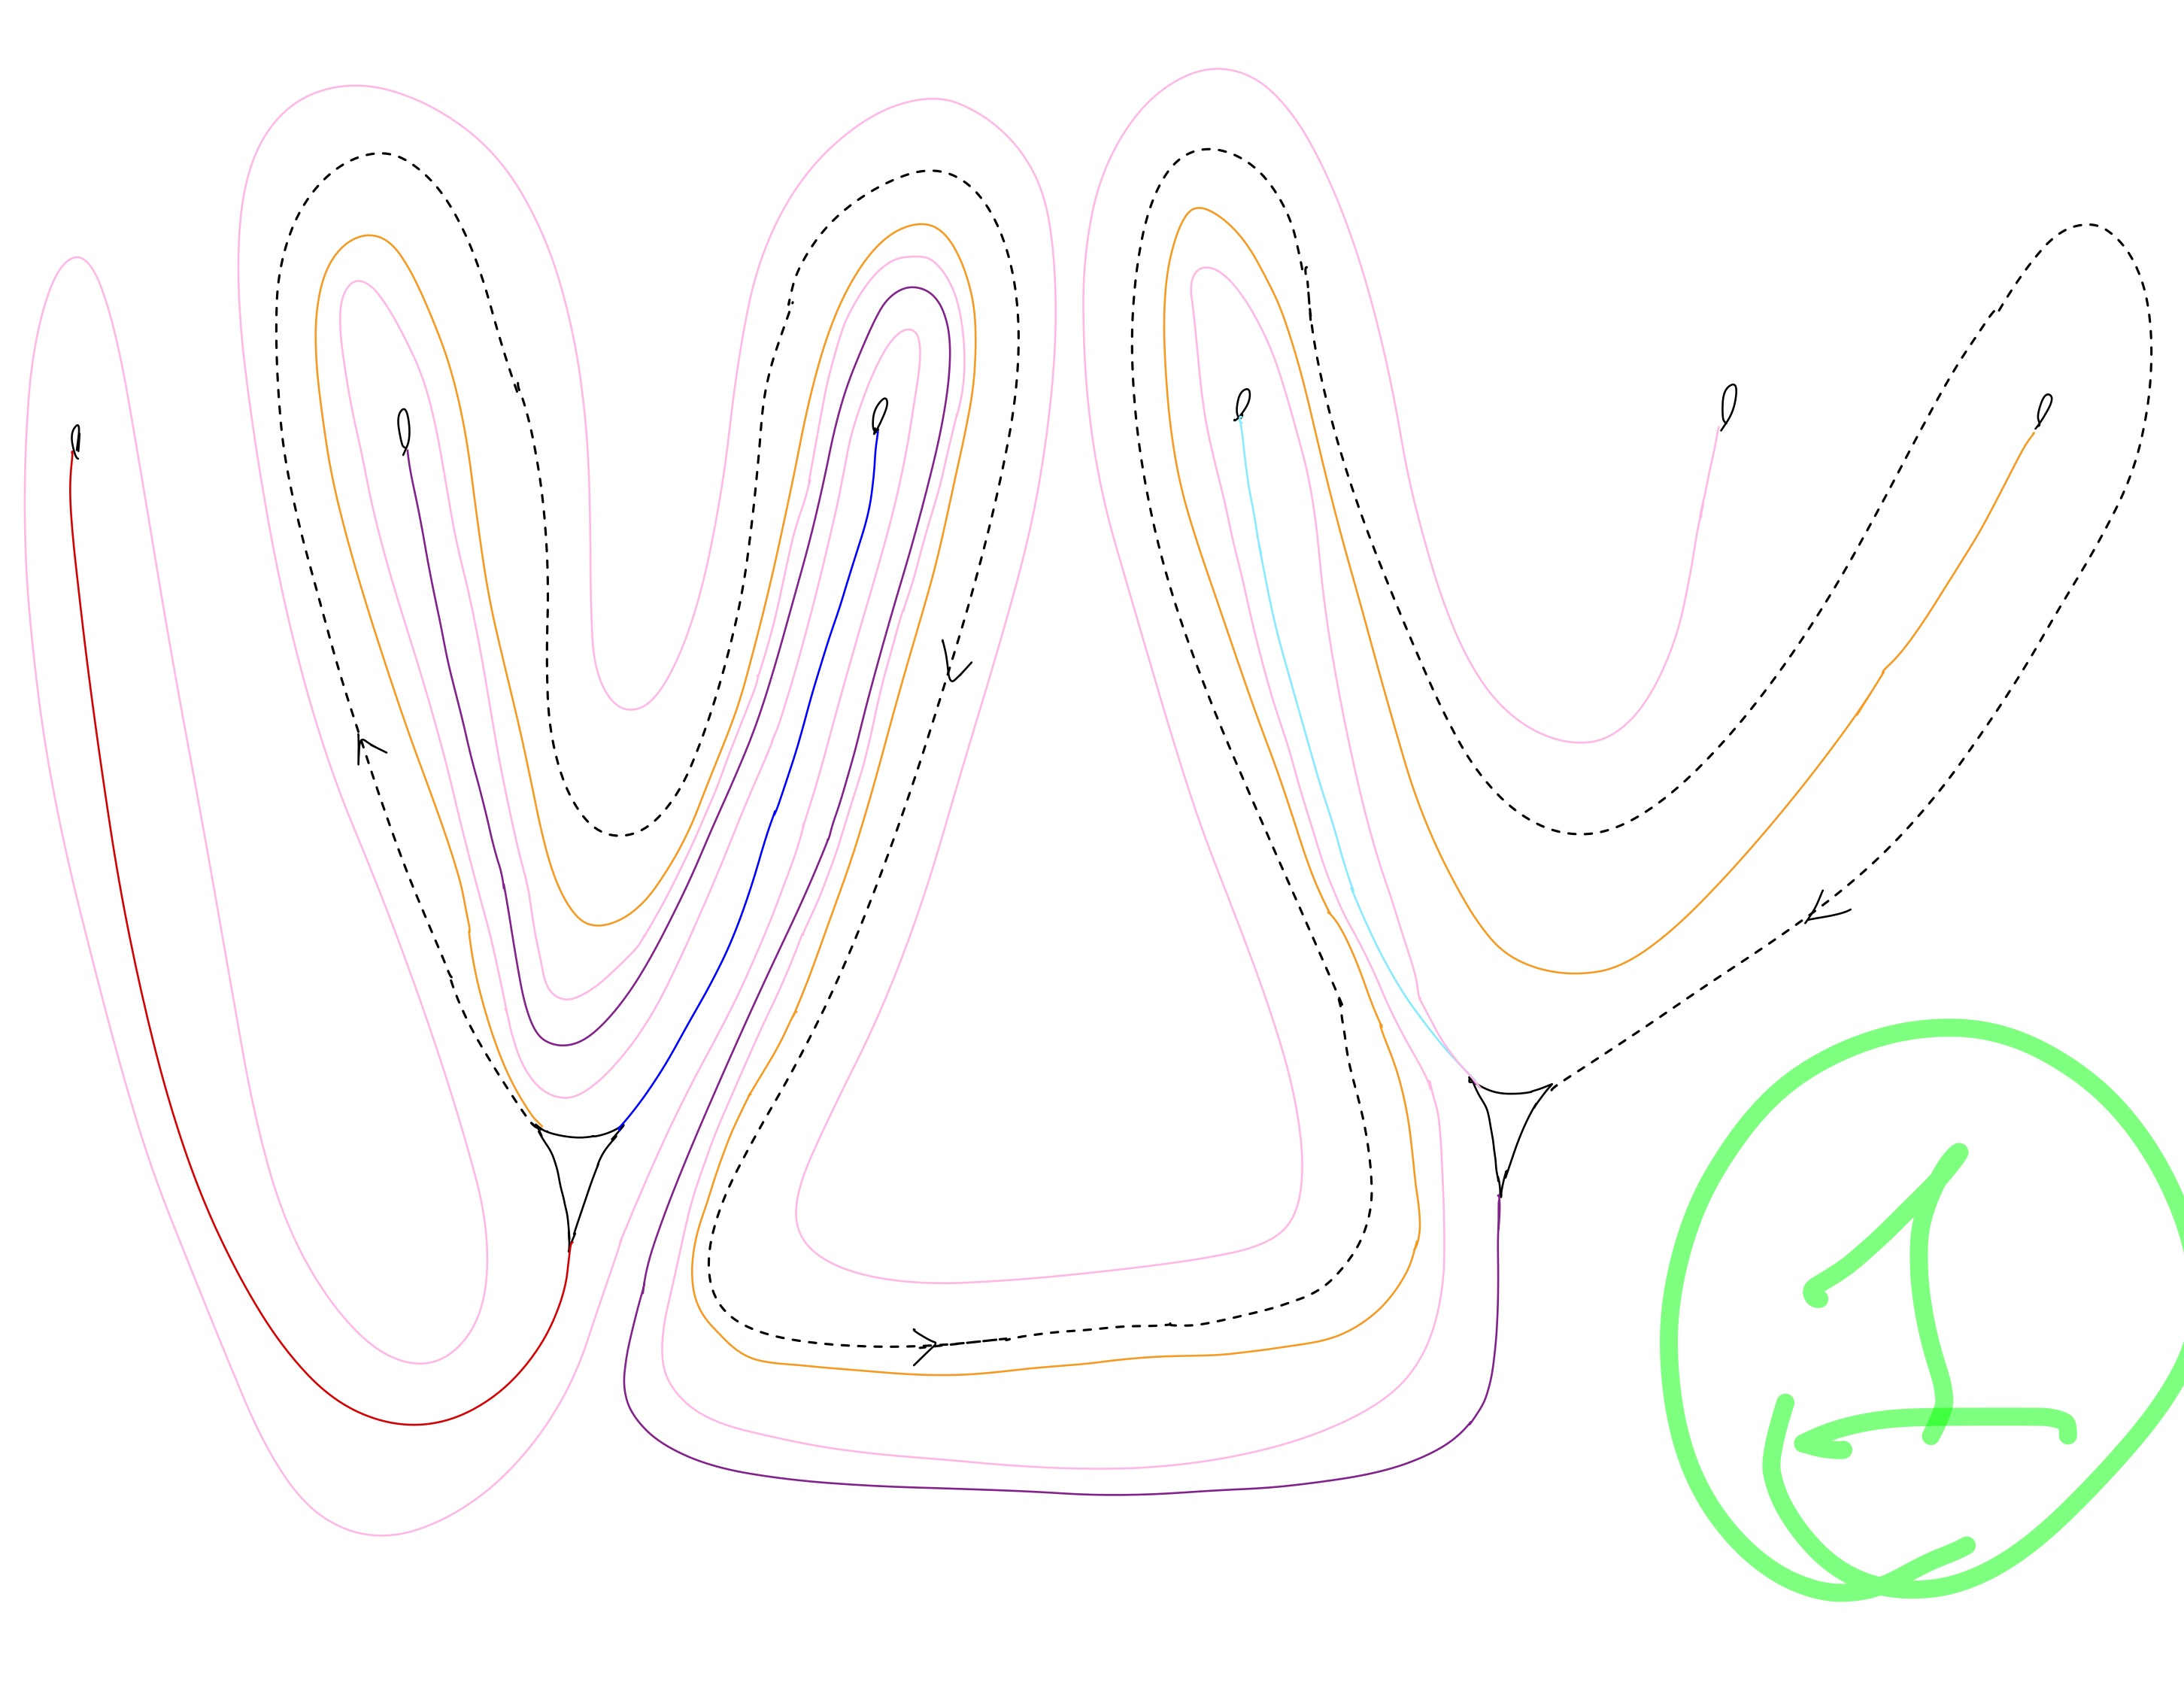
\includegraphics[width=\linewidth, height=0.45\textheight, keepaspectratio]{figures_braid/figures_track_1/Track 1 Braid 1 Flute-1.jpg}
    \caption{Train Track Map Candidate Family 1 (Flute) of Track 1.}
    \label{fig:track1_braid_b1_1_map}
\end{figure*}

The inverse of the following braid carries this family of train track maps:
\[
b_1^1 = \sigma_{2}^{-1} \sigma_{4} \sigma_{3} \sigma_{2} \sigma_{1} \sigma_{2}^{-1} \sigma_{3}^{-1} \sigma_{4}^{-1} \sigma_{5}^{-1} \sigma_{2}^{-1} \sigma_{3}^{-1} \sigma_{4}^{-1} \sigma_{1}^{-1} \sigma_{2}^{-1} \circ J \circ \Lambda_6
\]

This is shown in Figure \ref{fig:track1_braid_b1_1}.

\begin{figure*}[p]
    \centering
    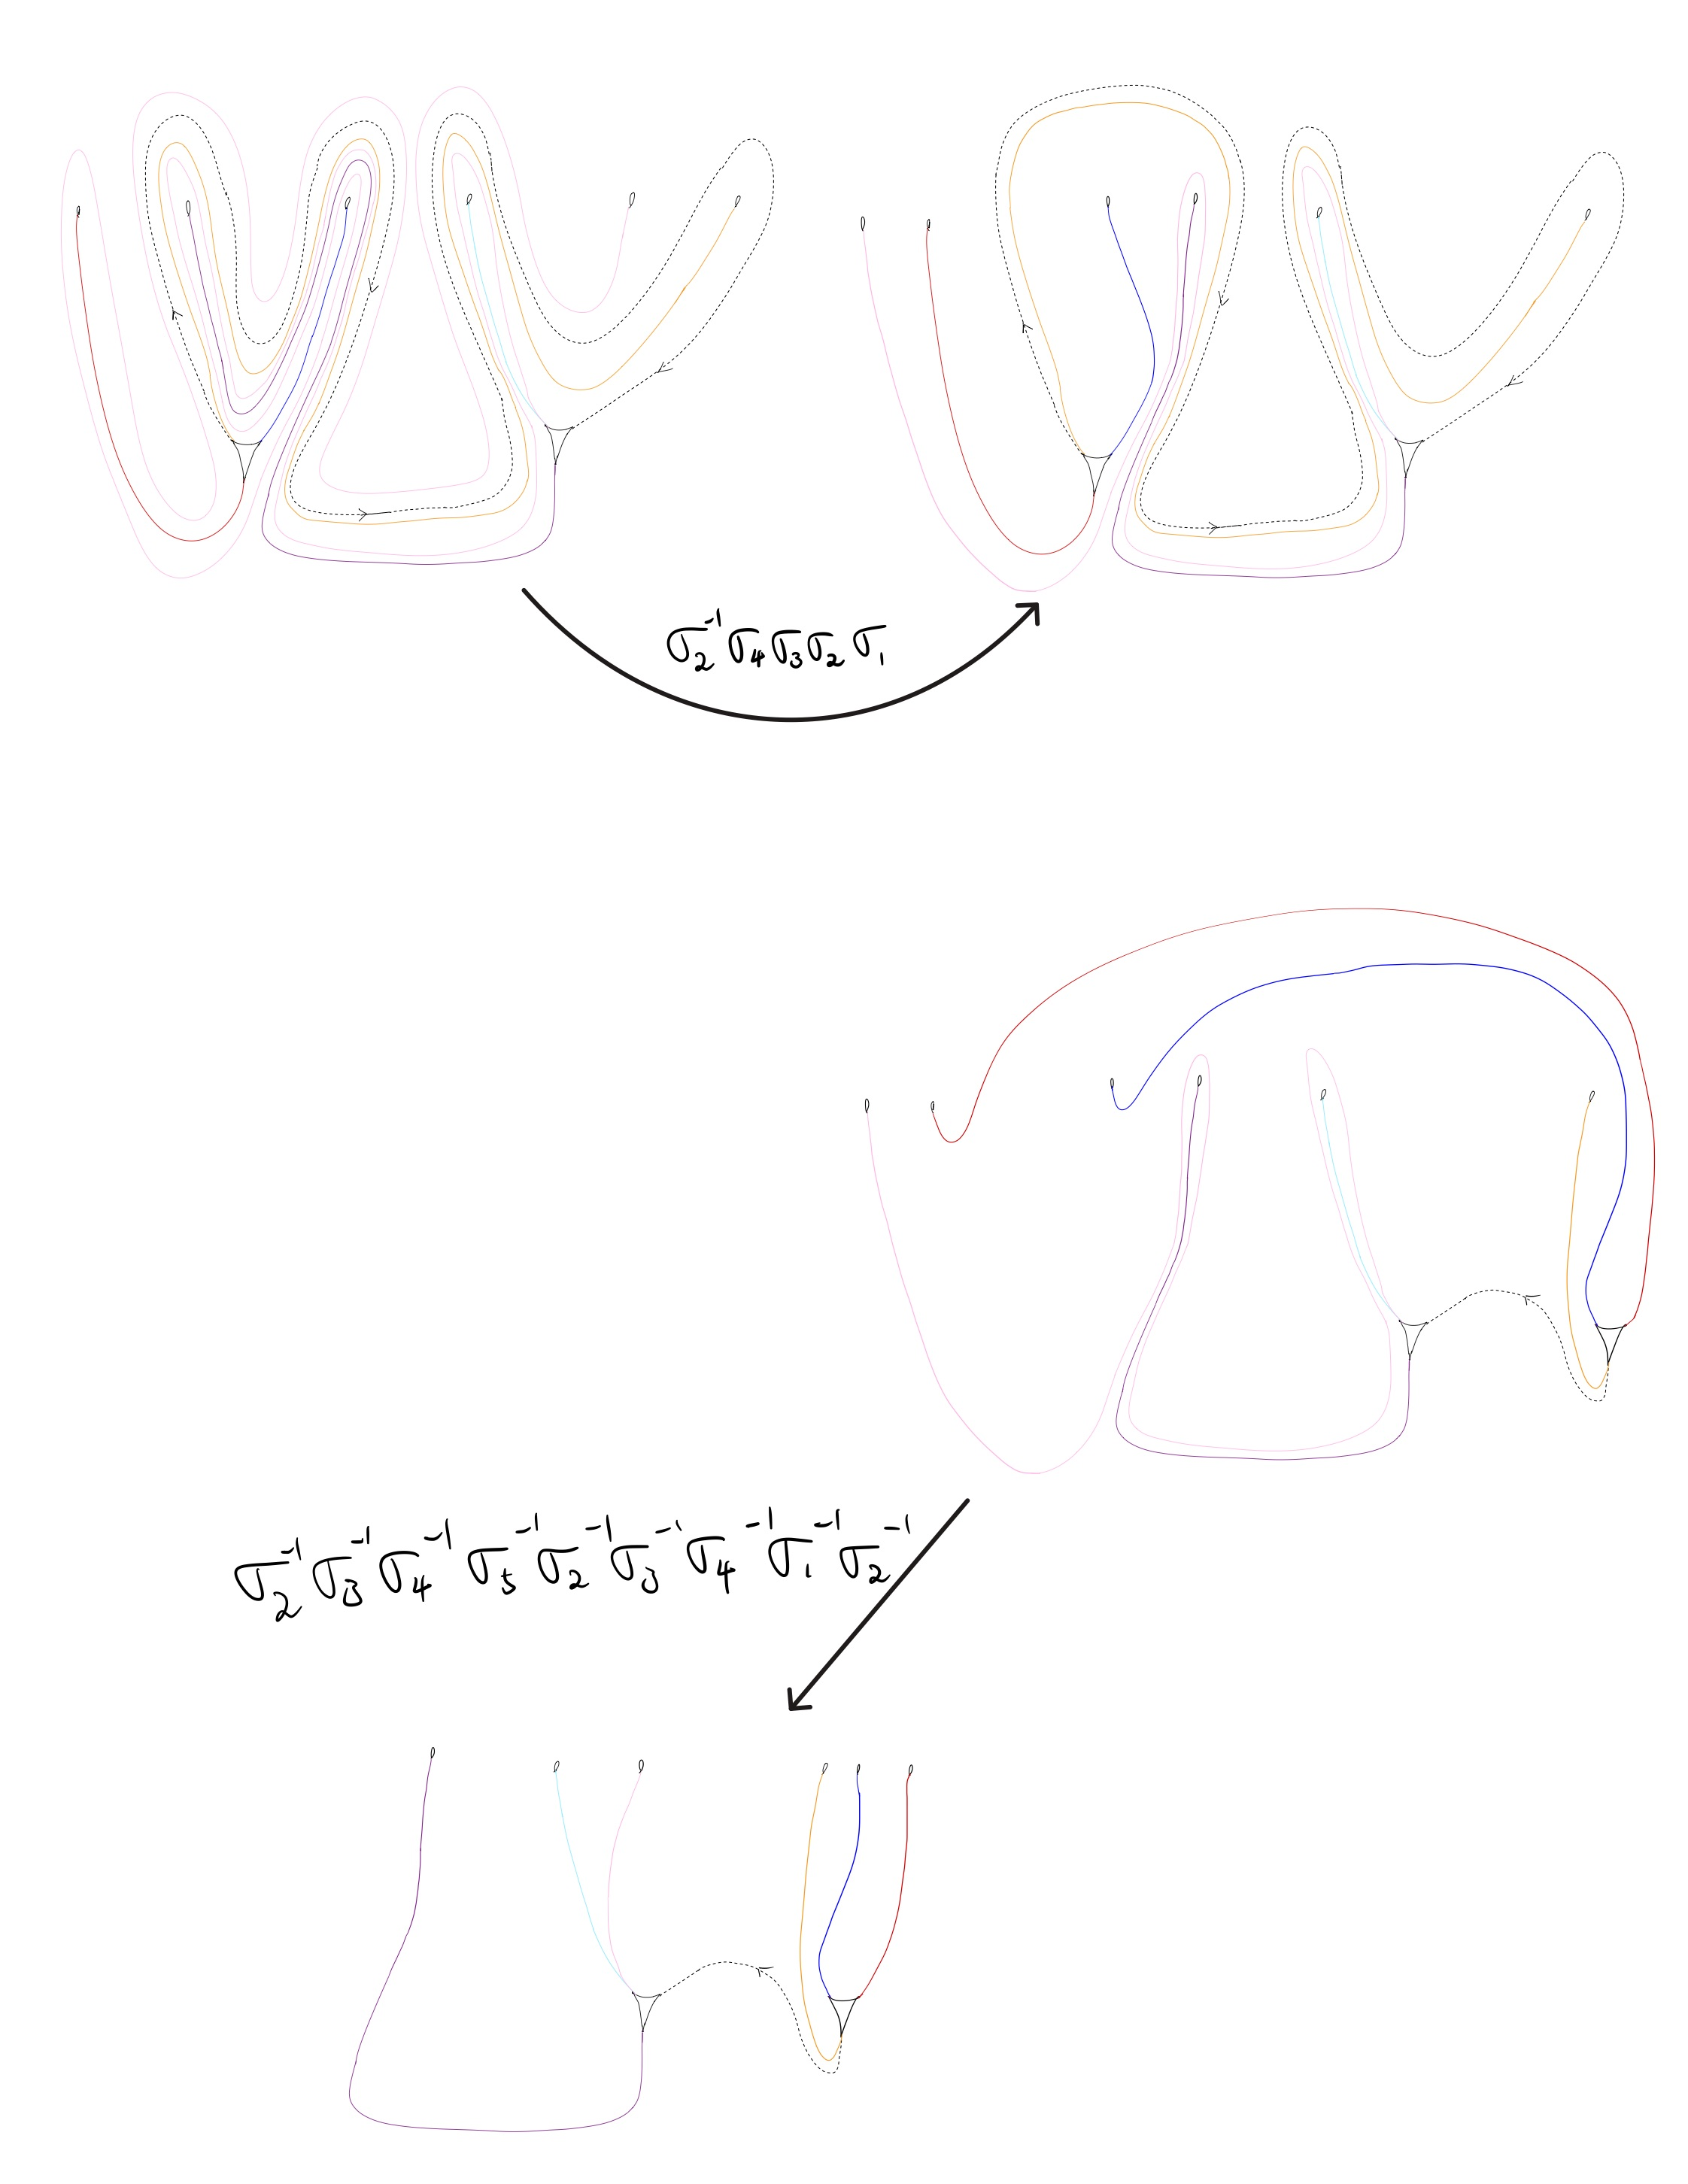
\includegraphics[width=\linewidth, height=0.45\textheight, keepaspectratio]{figures_braid/figures_track_1/Track 1 Braid 1 Flute-2.jpg}\\
    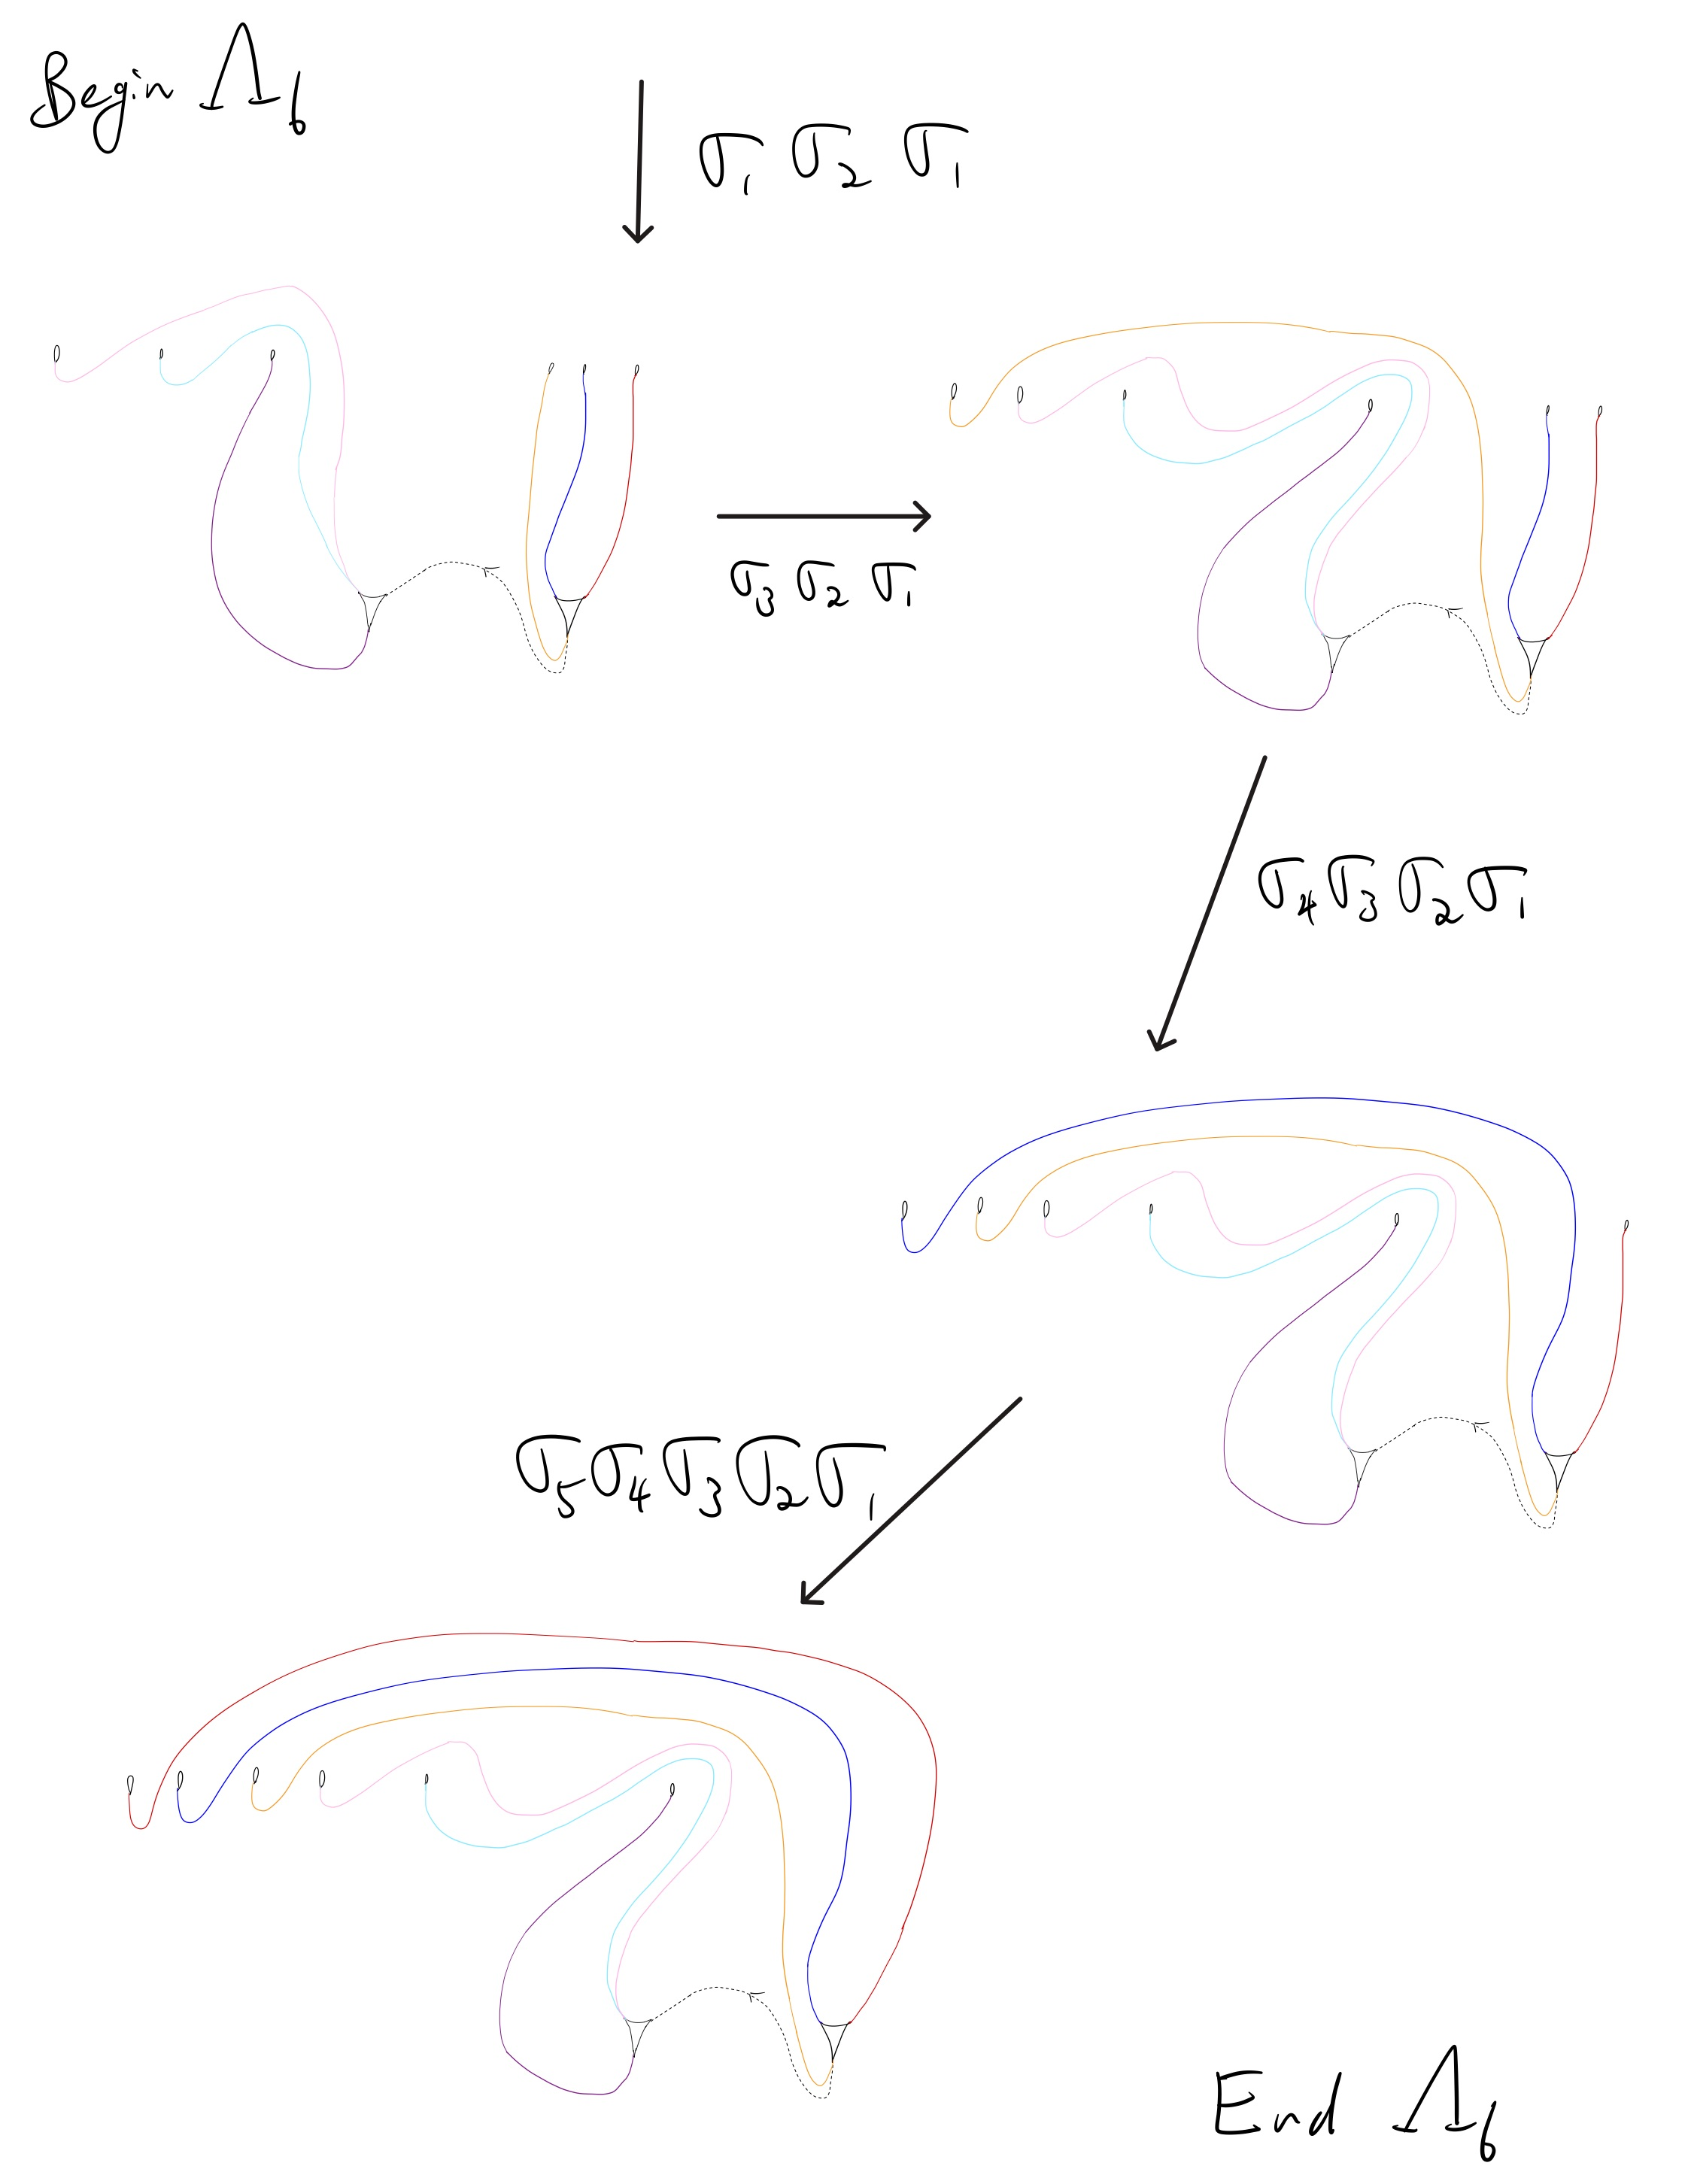
\includegraphics[width=\linewidth, height=0.45\textheight, keepaspectratio]{figures_braid/figures_track_1/Track 1 Braid 1 Flute-3.jpg}
    \caption{This sequence shows the inverse of the braid $b_1^1$ carries Train Track Candidate Family 1.}
    \label{fig:track1_braid_b1_1}
\end{figure*}

\clearpage

\section{Candidate Family 2 (Dolphin)}\label{sec:track1_dolphin}
Train Track Map Candidate Family 2 of Track 1 is shown in Figure \ref{fig:track1_braid_b1_2_map}. See \ref{Dolphin} for details.

\begin{figure*}[ht]
    \centering
    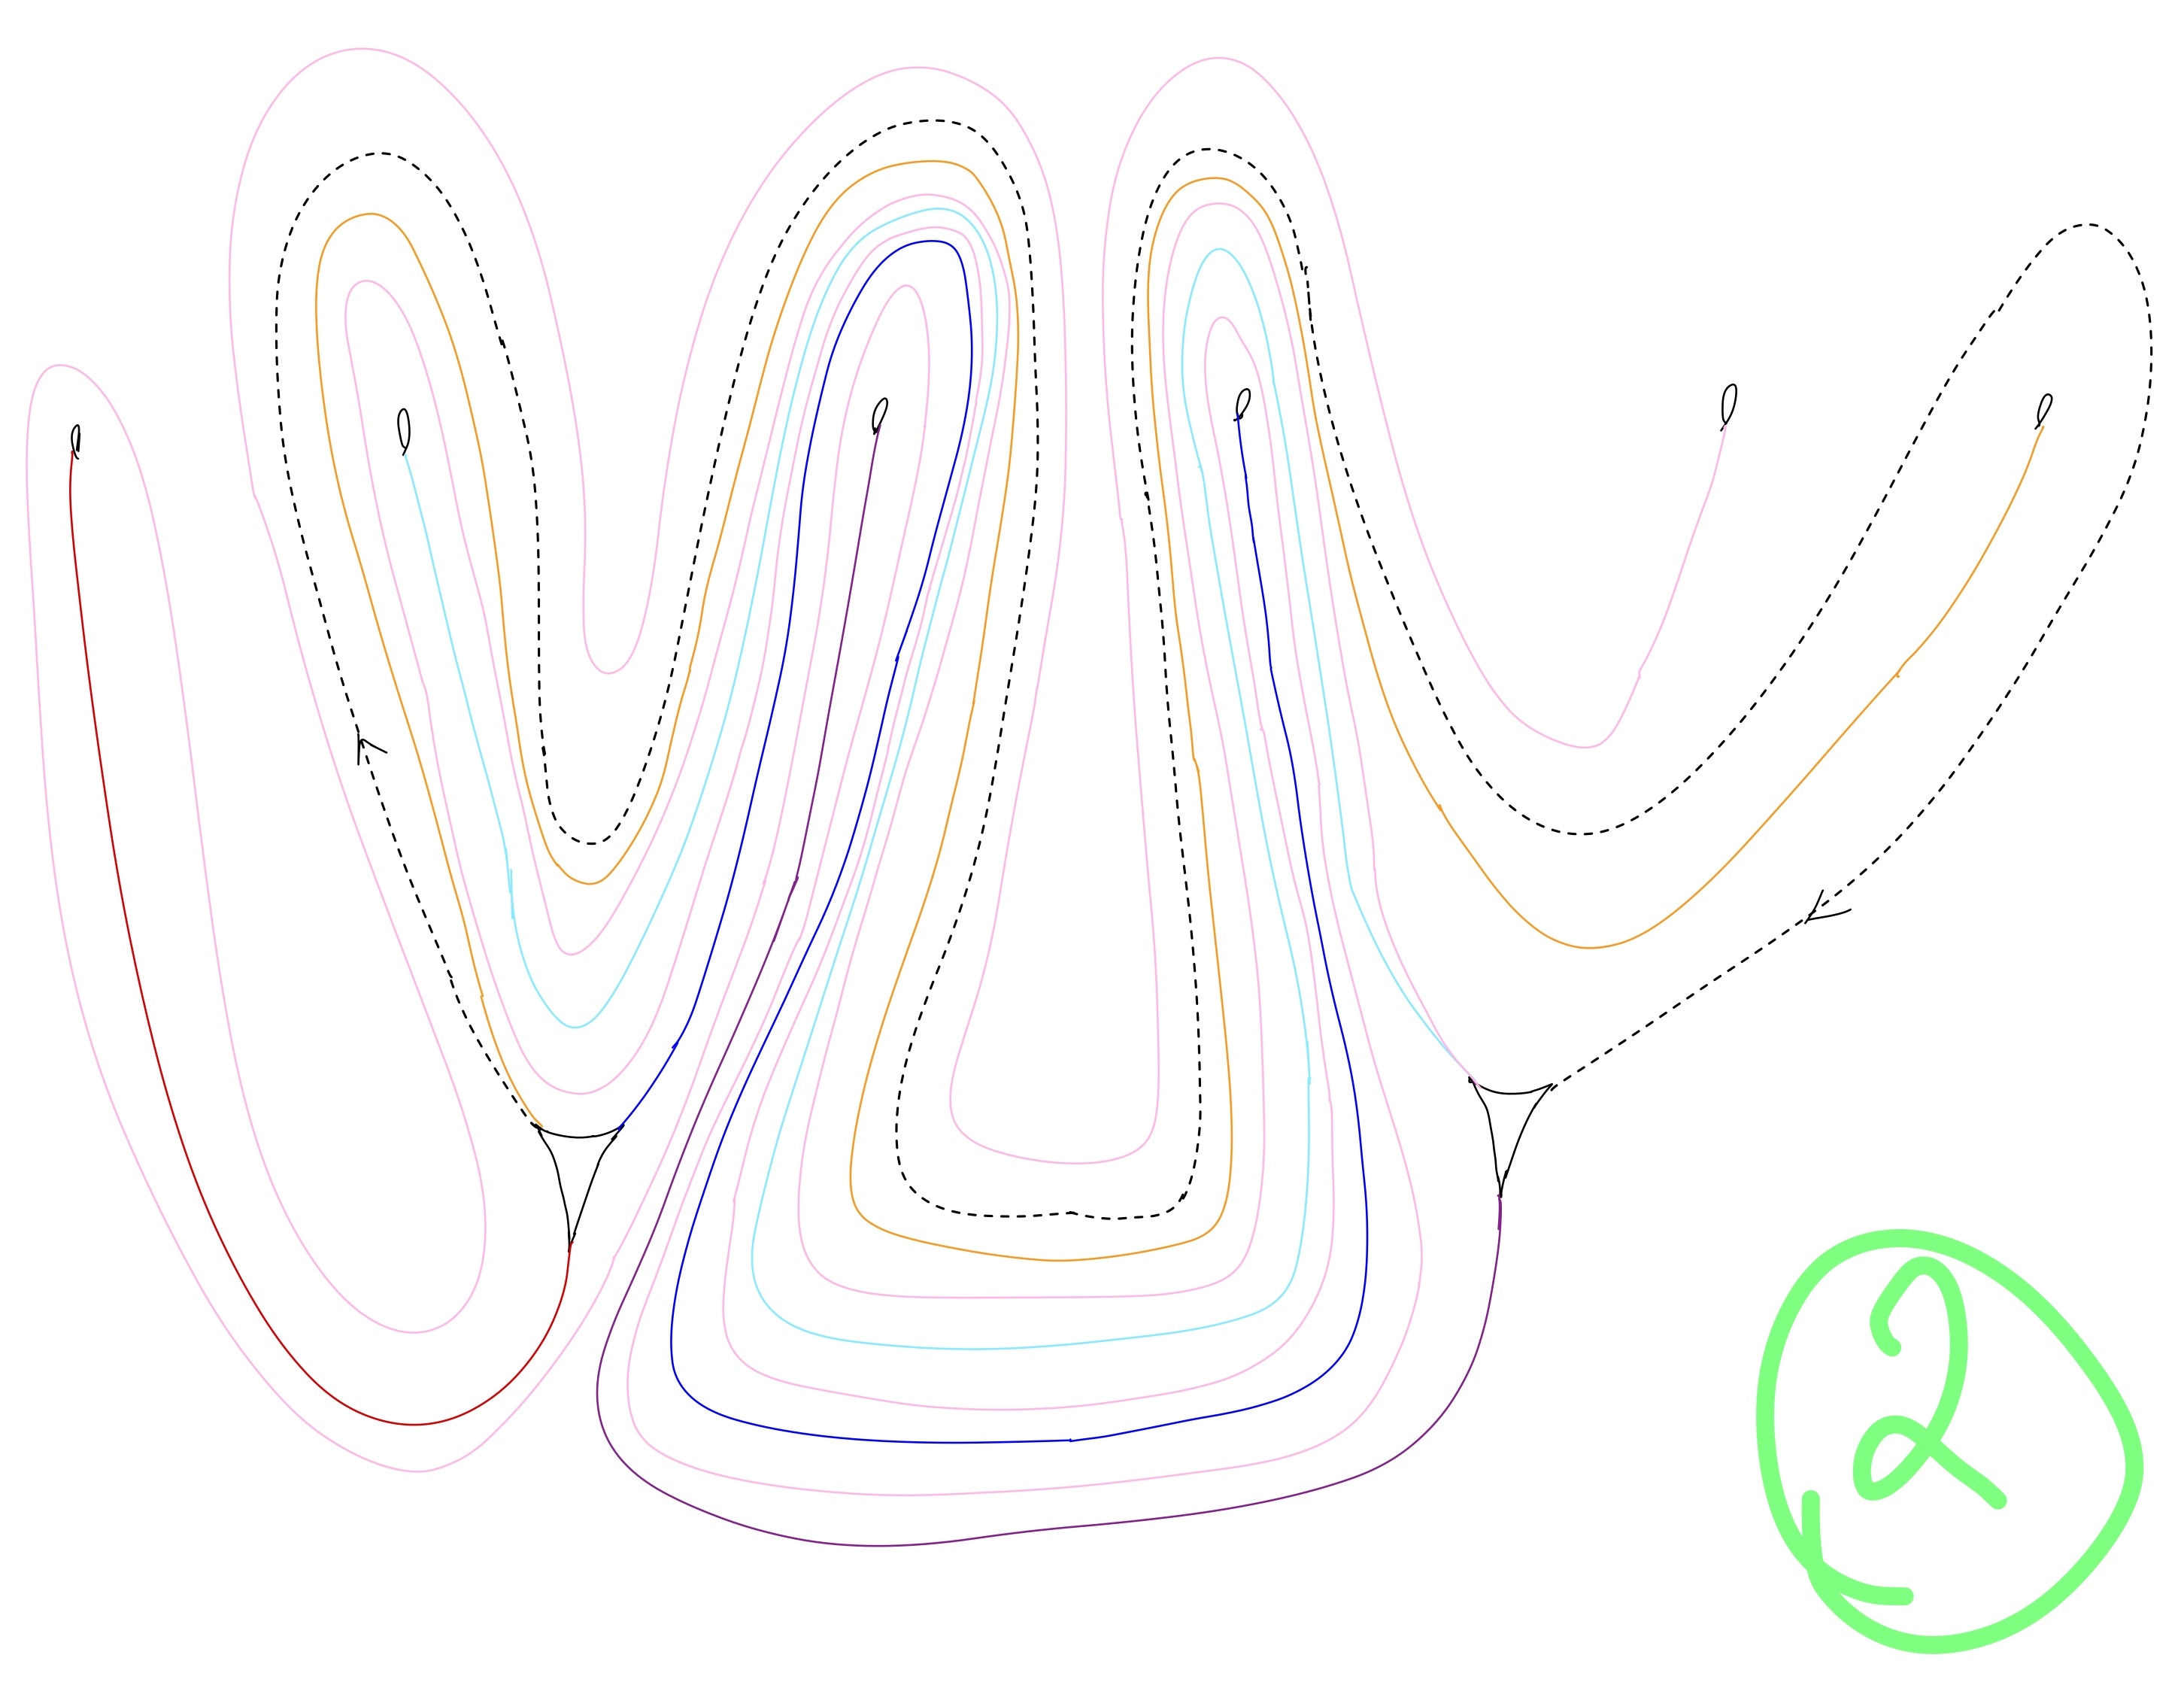
\includegraphics[width=\linewidth, height=0.45\textheight, keepaspectratio]{figures_braid/figures_track_1/Track 1 Braid 2 Dolphin-1.jpg}
    \caption{Train Track Map Candidate Family 2 (Dolphin) of Track 1.}
    \label{fig:track1_braid_b1_2_map}
\end{figure*}

The inverse of the following braid carries this family of train track maps:
\[
b_2^1 = \sigma_{4} \sigma_{3} \sigma_{2} \sigma_{1} \sigma_{5} \sigma_{4} \sigma_{3} \sigma_{4}^{-1} \sigma_{5}^{-1} \sigma_{4} \sigma_{2}^{-1} \sigma_{3}^{-1} \sigma_{4}^{-1} \sigma_{5}^{-1} \sigma_{2}^{-1} \sigma_{2}^{-1} \sigma_{3}^{-1} \sigma_{4}^{-1} \sigma_{2}^{-1} \sigma_{3}^{-1} \sigma_{1}^{-1} \sigma_{2}^{-1} \circ J \circ \Lambda_6
\]

This is shown in Figure \ref{fig:track1_braid_b1_2}.

\begin{figure*}[p]
    \centering
    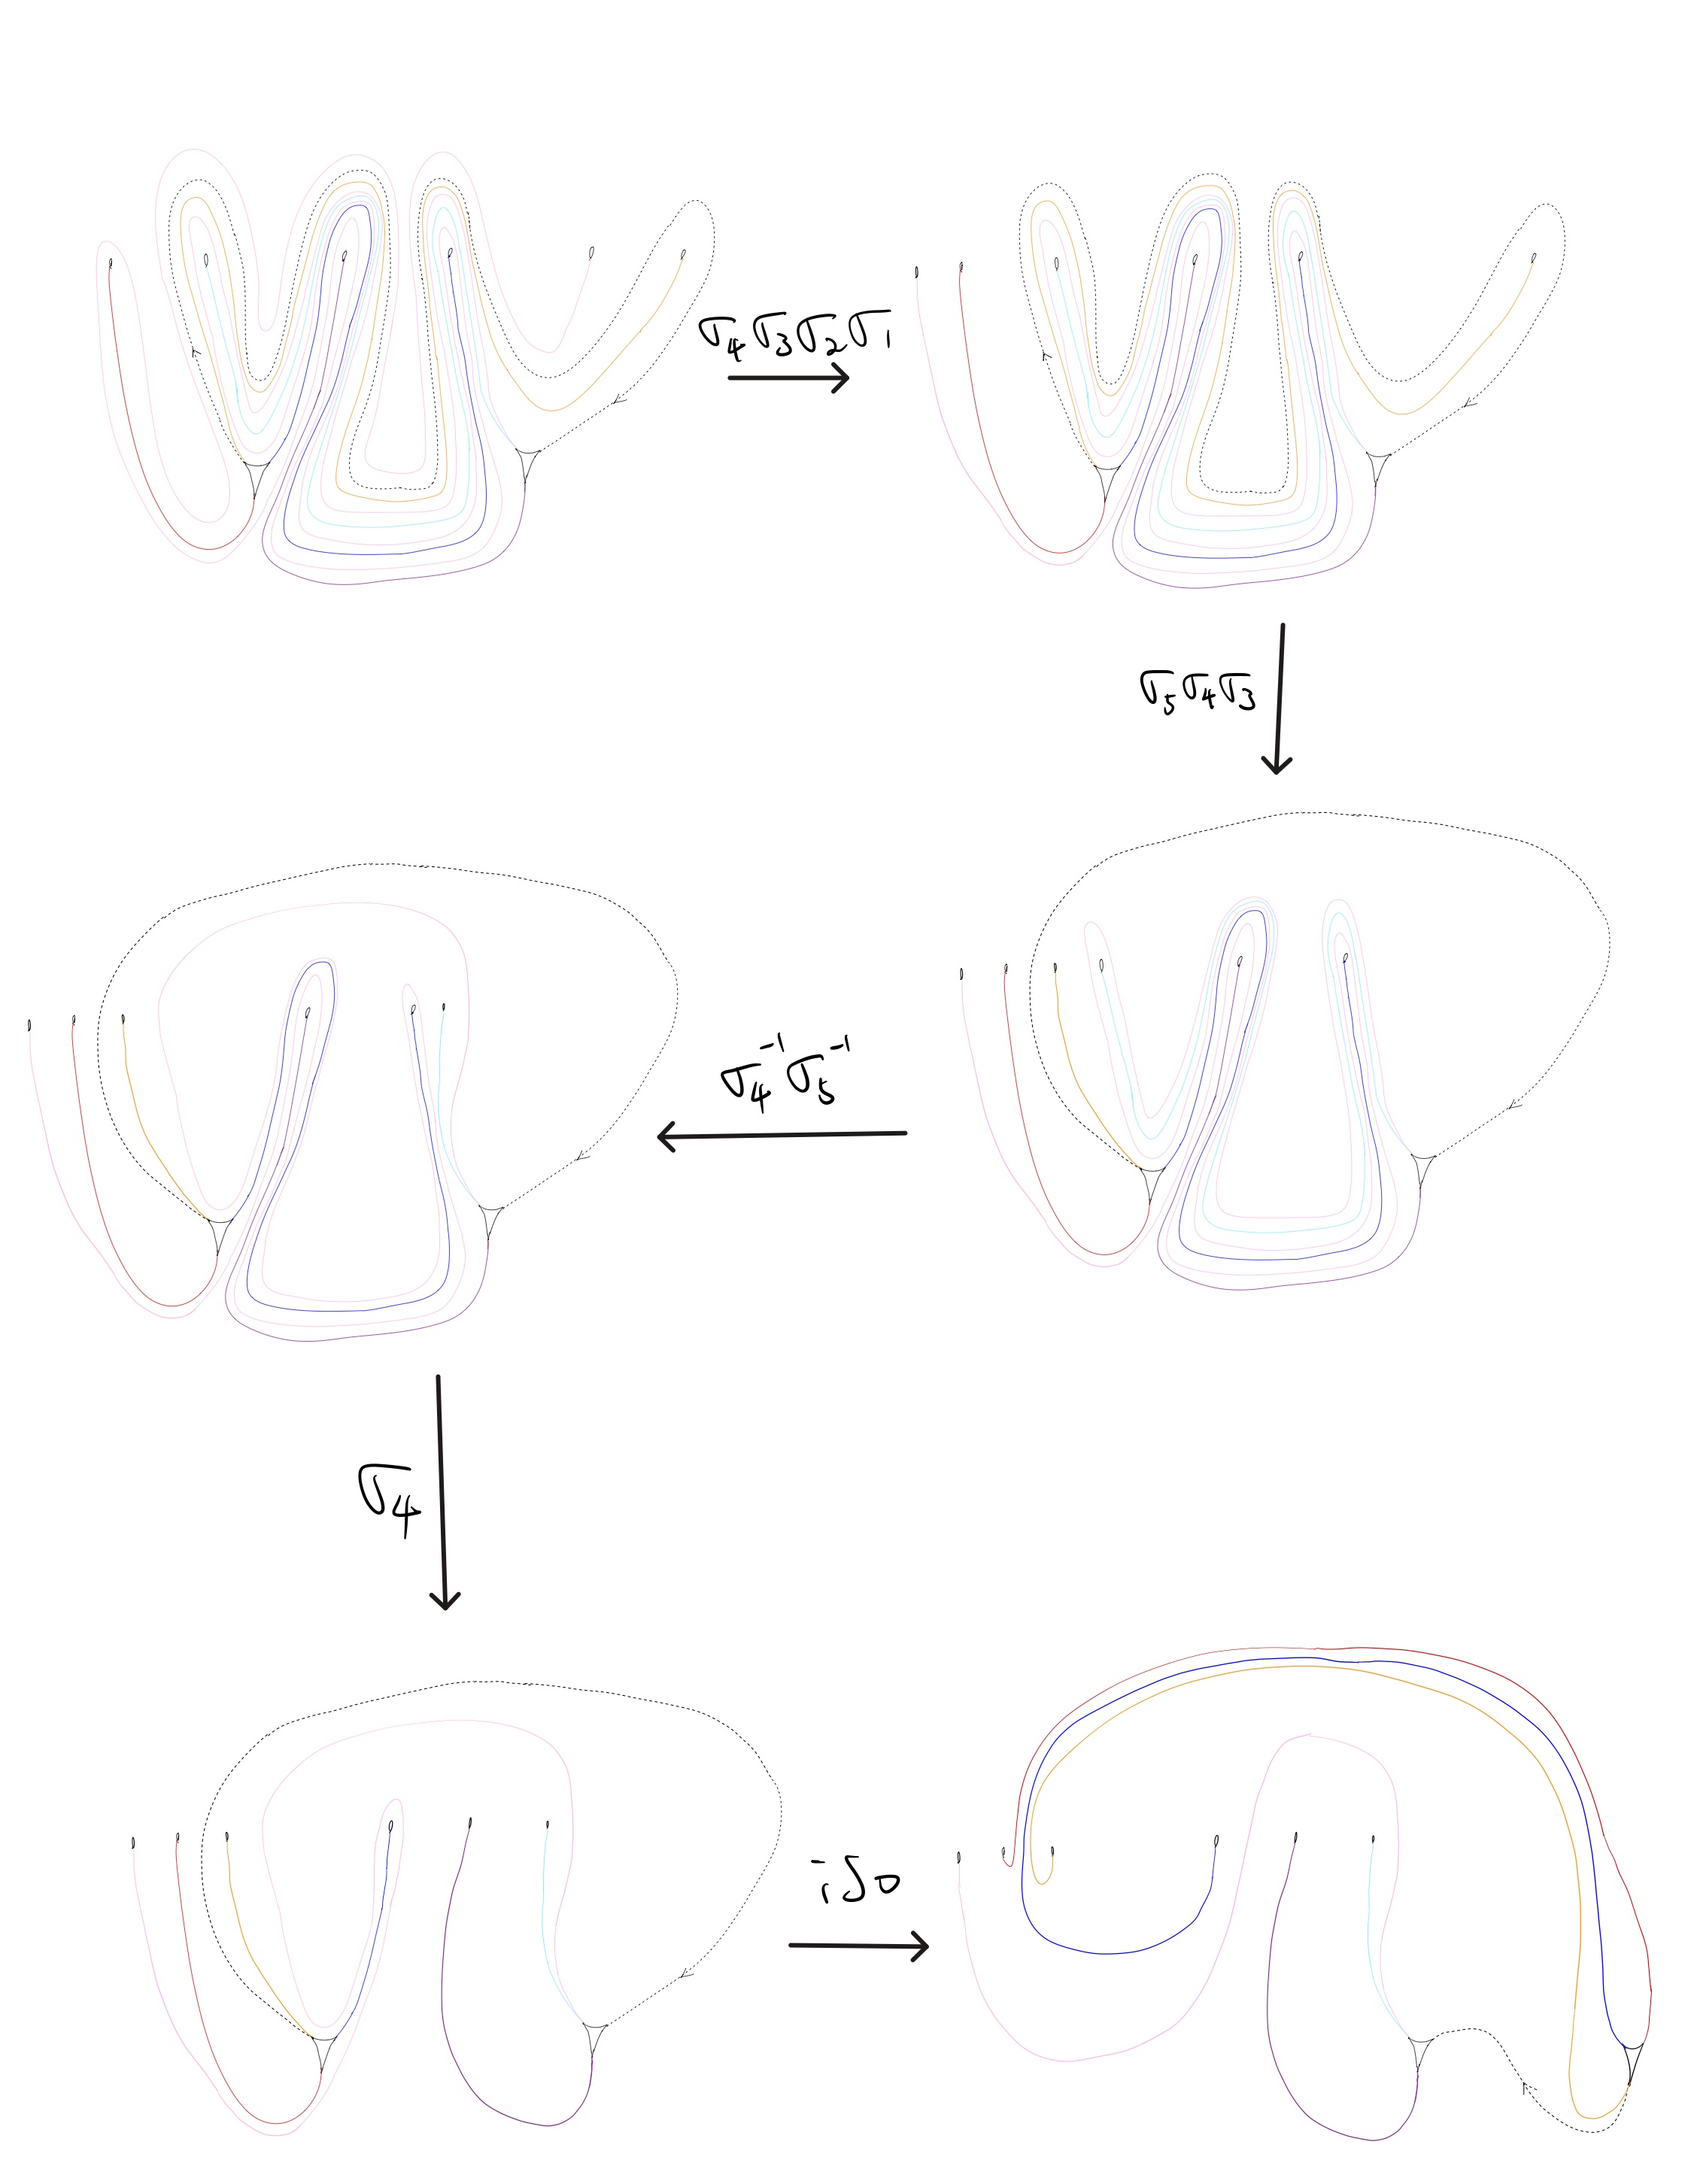
\includegraphics[width=\linewidth, height=0.45\textheight, keepaspectratio]{figures_braid/figures_track_1/Track 1 Braid 2 Dolphin-2.jpg}\\
    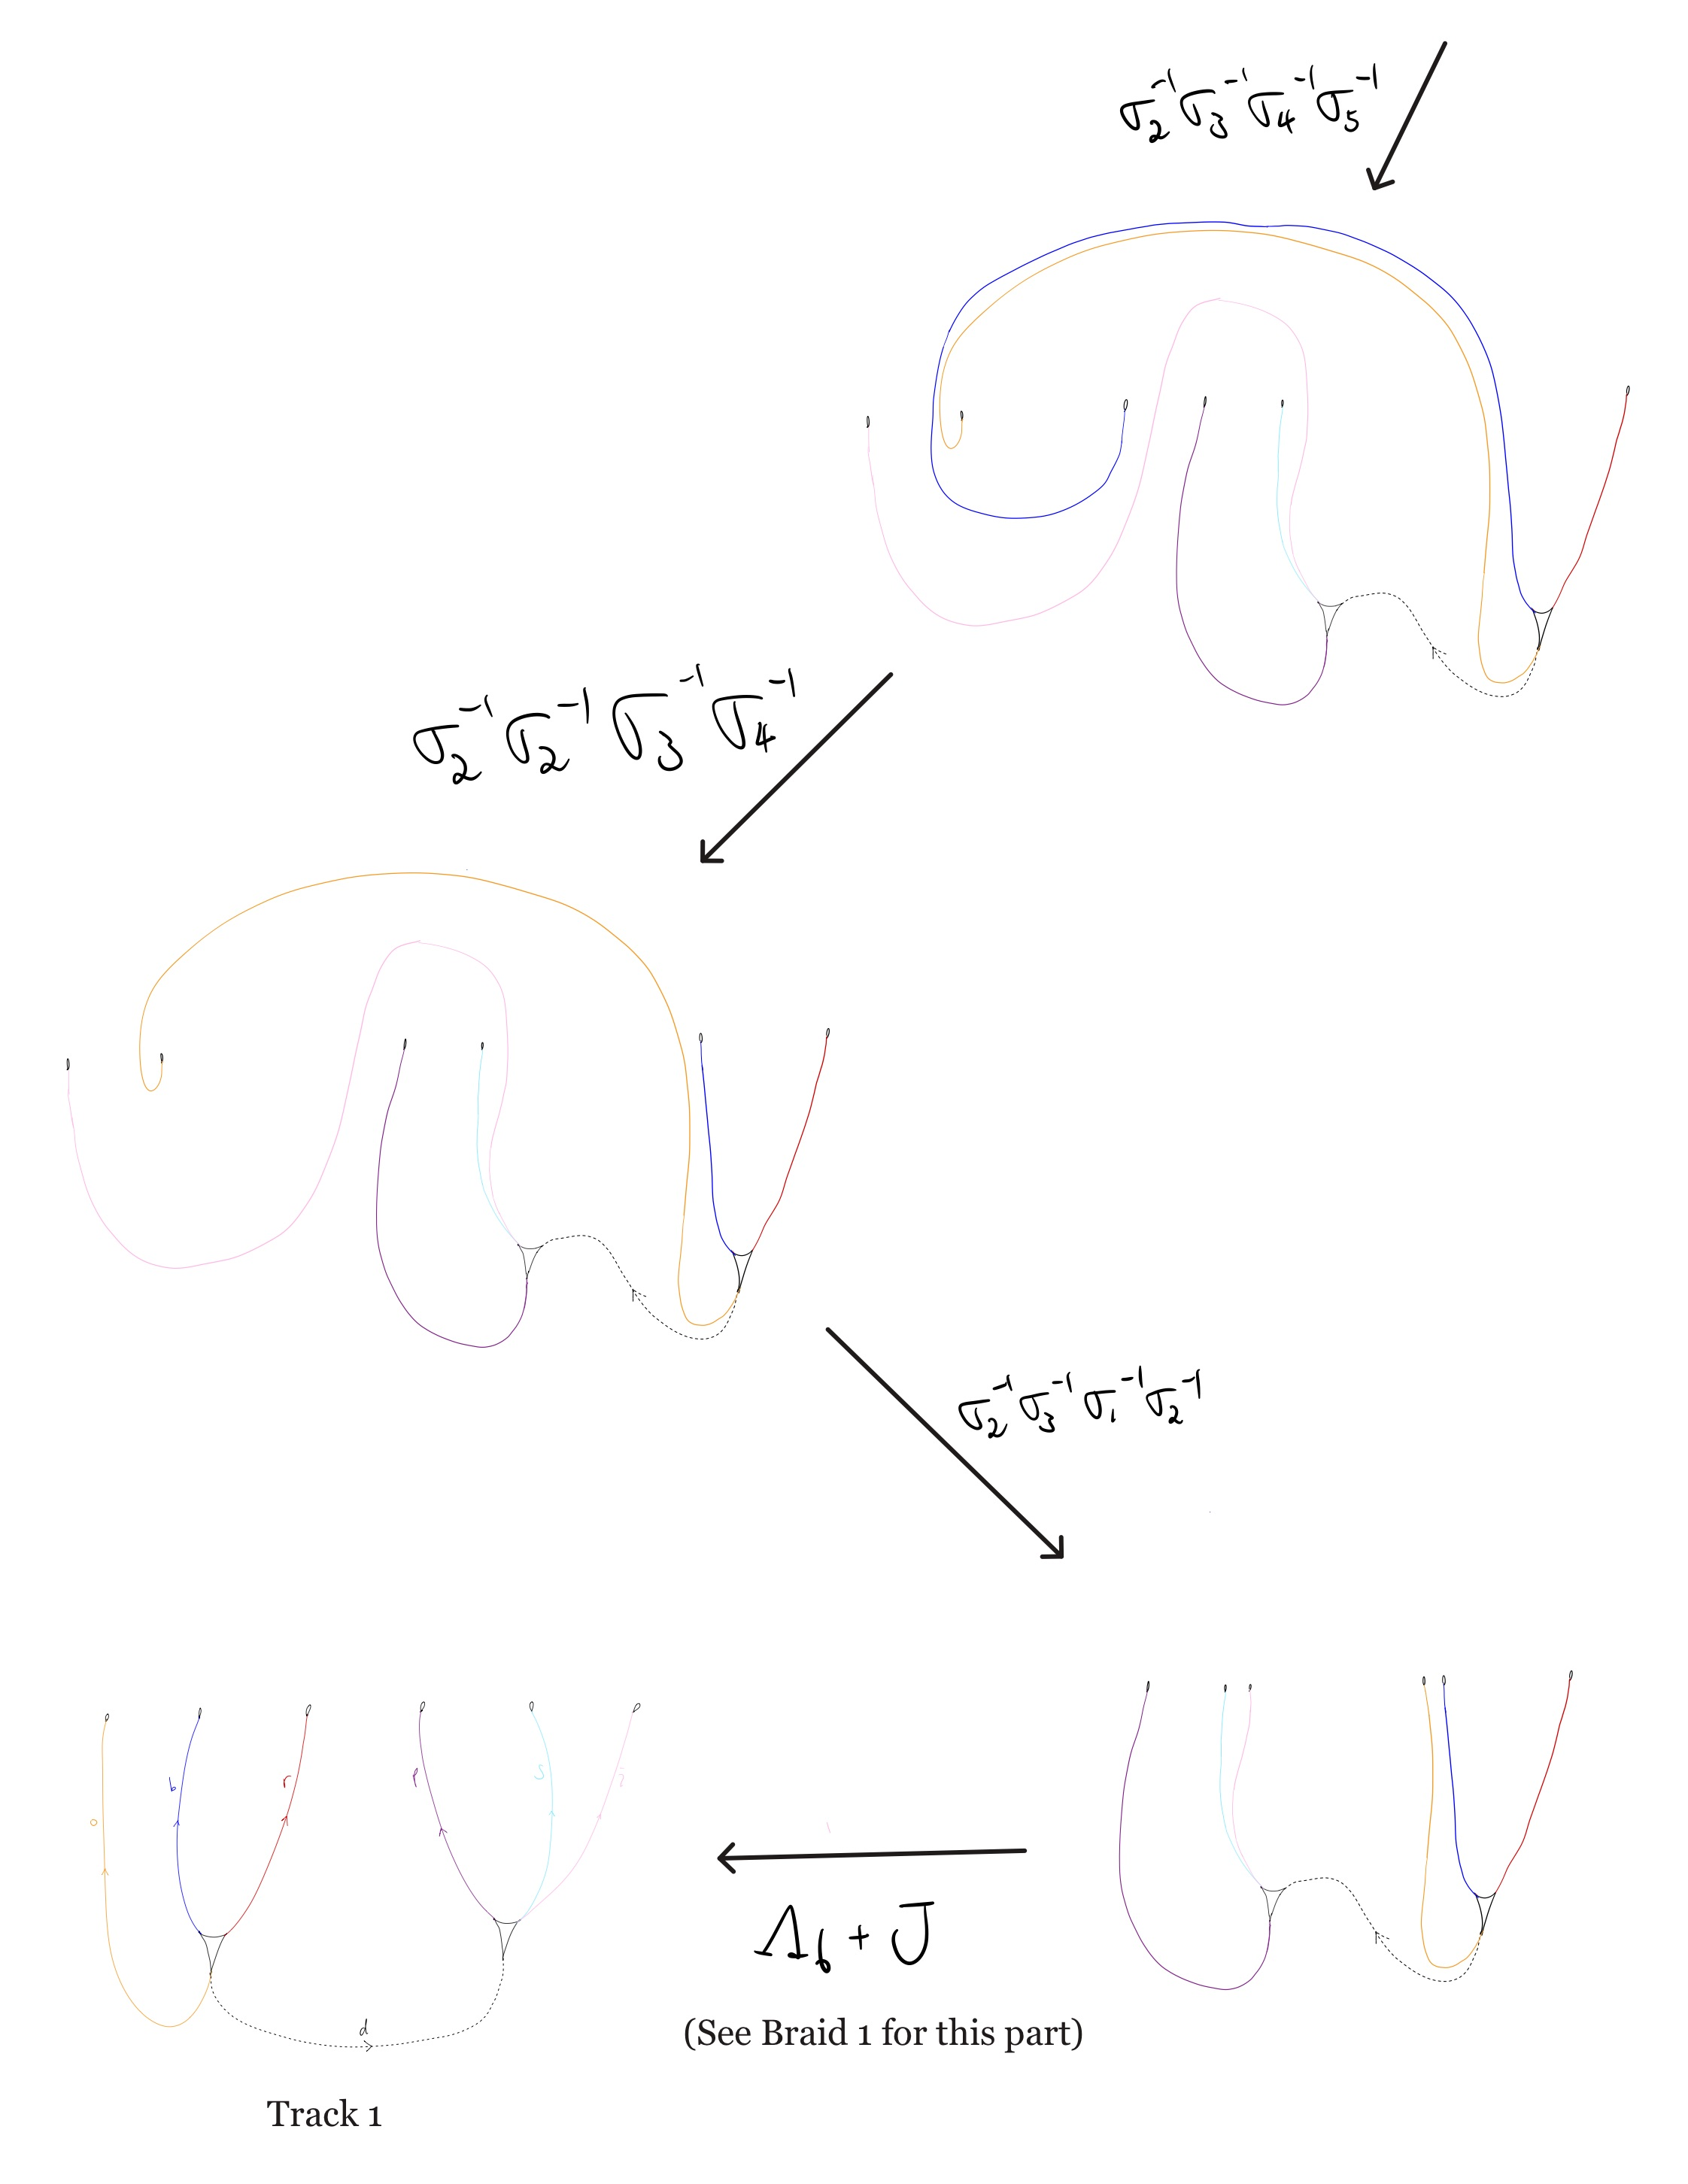
\includegraphics[width=\linewidth, height=0.45\textheight, keepaspectratio]{figures_braid/figures_track_1/Track 1 Braid 2 Dolphin-3.jpg}
    \caption{This sequence shows the inverse of the braid $b_2^1$ carries Train Track Candidate Family 2.}
    \label{fig:track1_braid_b1_2}
\end{figure*}

\clearpage

\section{Candidate Family 3 (Magpie)}\label{sec:track1_magpie}
Train Track Map Candidate Family 3 of Track 1 is shown in Figure \ref{fig:track1_braid_b1_3_map}. See \ref{Magpie} for details.

\begin{figure*}[ht]
    \centering
    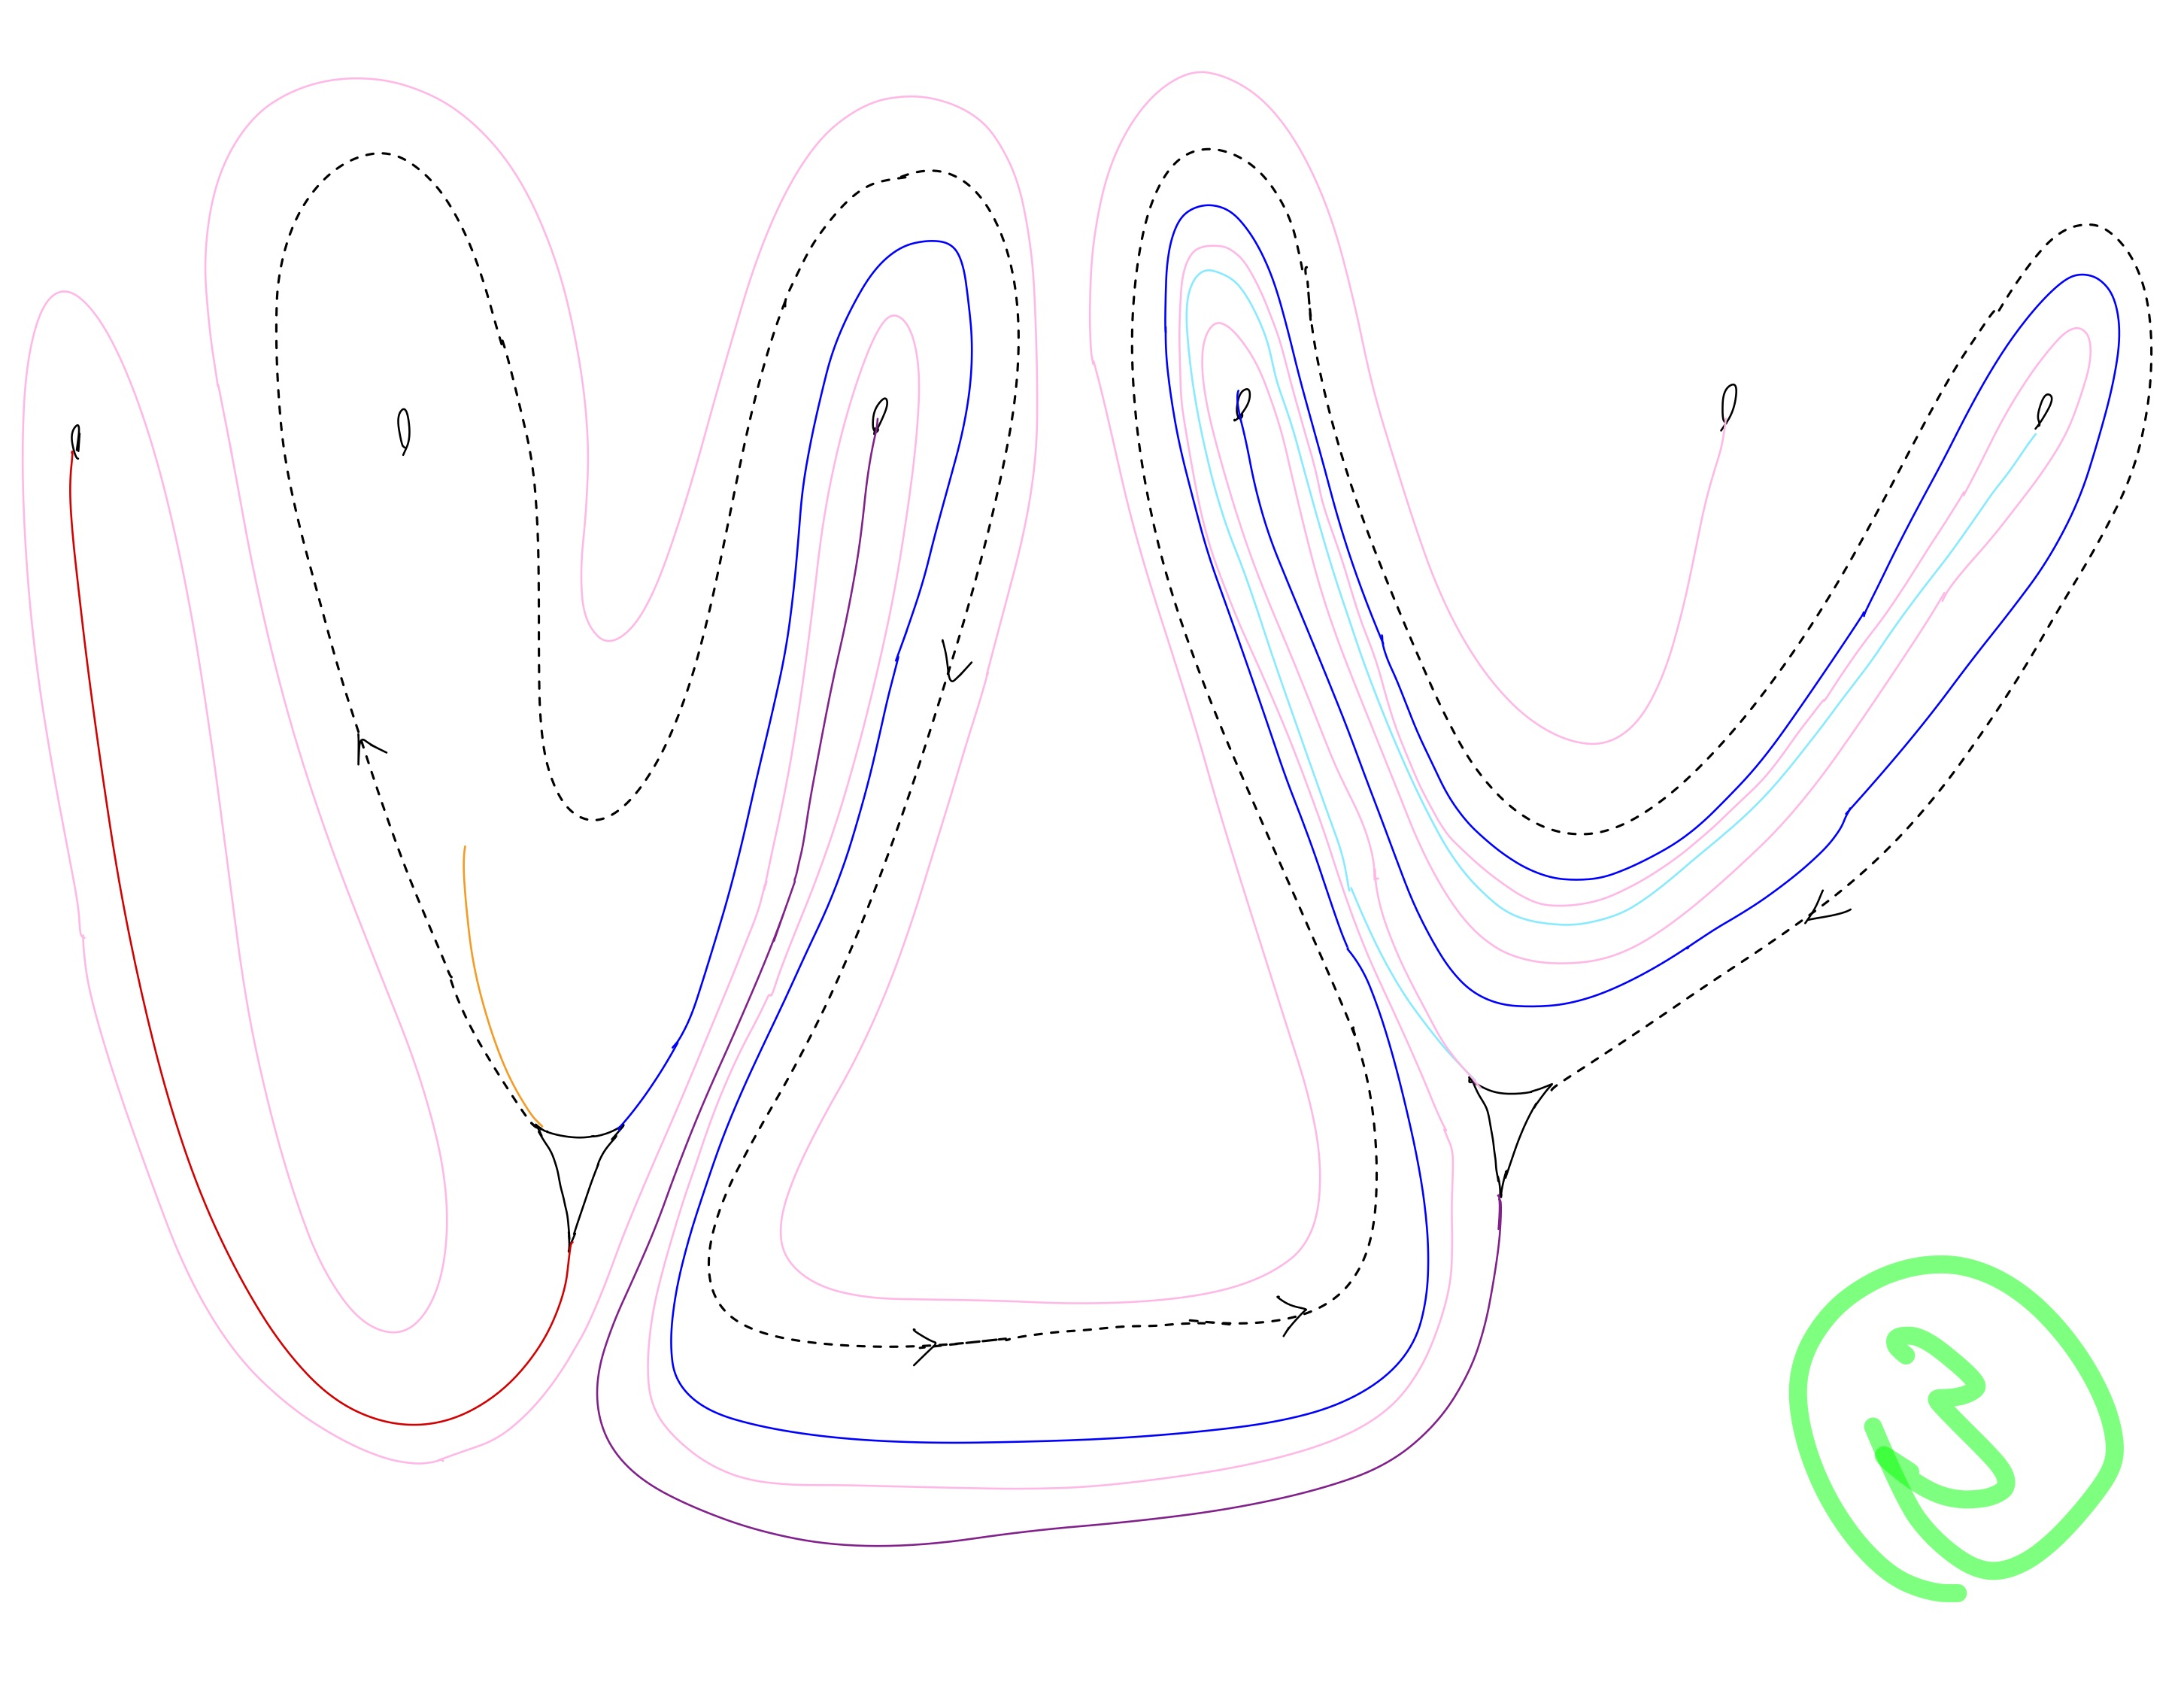
\includegraphics[width=\linewidth, height=0.45\textheight, keepaspectratio]{figures_braid/figures_track_1/Track 1 Braid 3 Magpie-1.jpg}
    \caption{Train Track Map Candidate Family 3 (Magpie) of Track 1.}
    \label{fig:track1_braid_b1_3_map}
\end{figure*}

The inverse of the following braid carries this family of train track maps:
\[
b_3^1 = \sigma_{4} \sigma_{3} \sigma_{2} \sigma_{1} \sigma_{5}^k \sigma_{5} \sigma_{4} \sigma_{2}^{-1} \sigma_{3}^{-1} \sigma_{4}^{-1} \sigma_{5}^{-1} \sigma_{2}^{-1} \sigma_{2}^{-1} \sigma_{3}^{-1} \sigma_{4}^{-1} \sigma_{2}^{-1} \sigma_{3}^{-1} \sigma_{1}^{-1} \sigma_{2}^{-1} \circ J \circ \Lambda_6
\]
where $k \geq 1$ ($k \in \mathbb{Z}$) is the twisting parameter. This is shown in Figure \ref{fig:track1_braid_b1_3}.

\begin{figure*}[p]
    \centering
    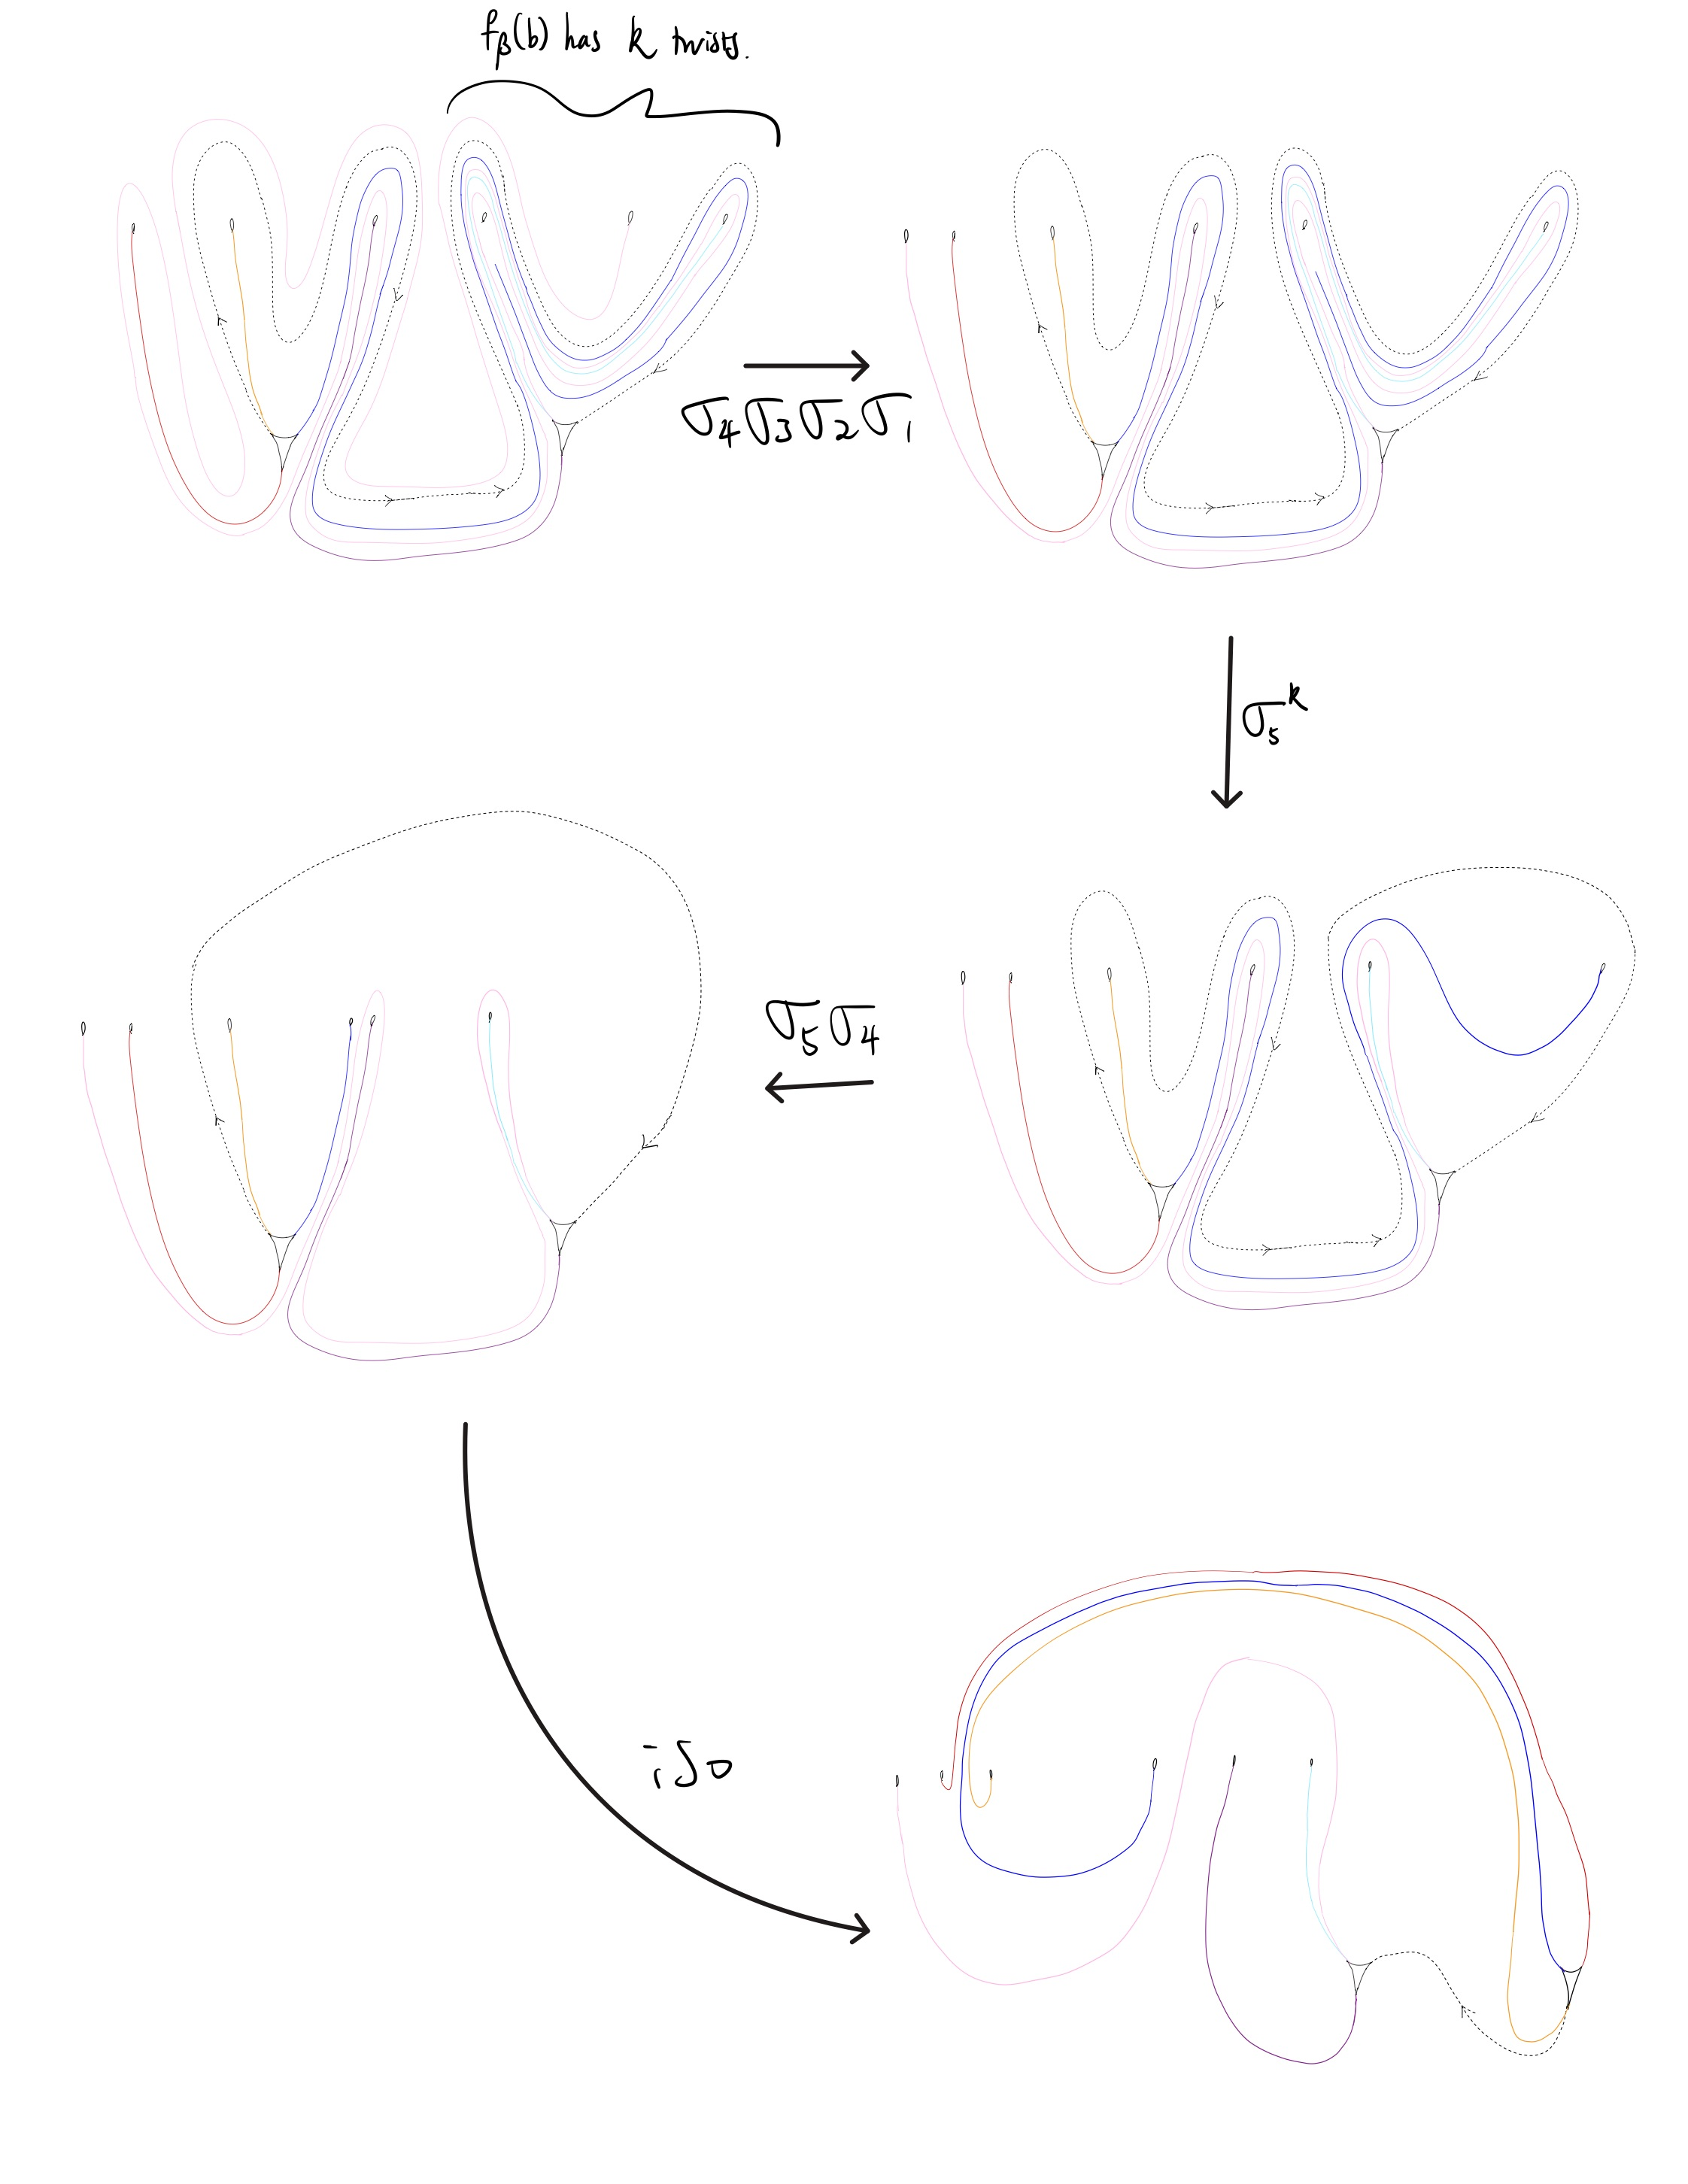
\includegraphics[width=\linewidth, height=0.45\textheight, keepaspectratio]{figures_braid/figures_track_1/Track 1 Braid 3 Magpie-2.jpg}\\
    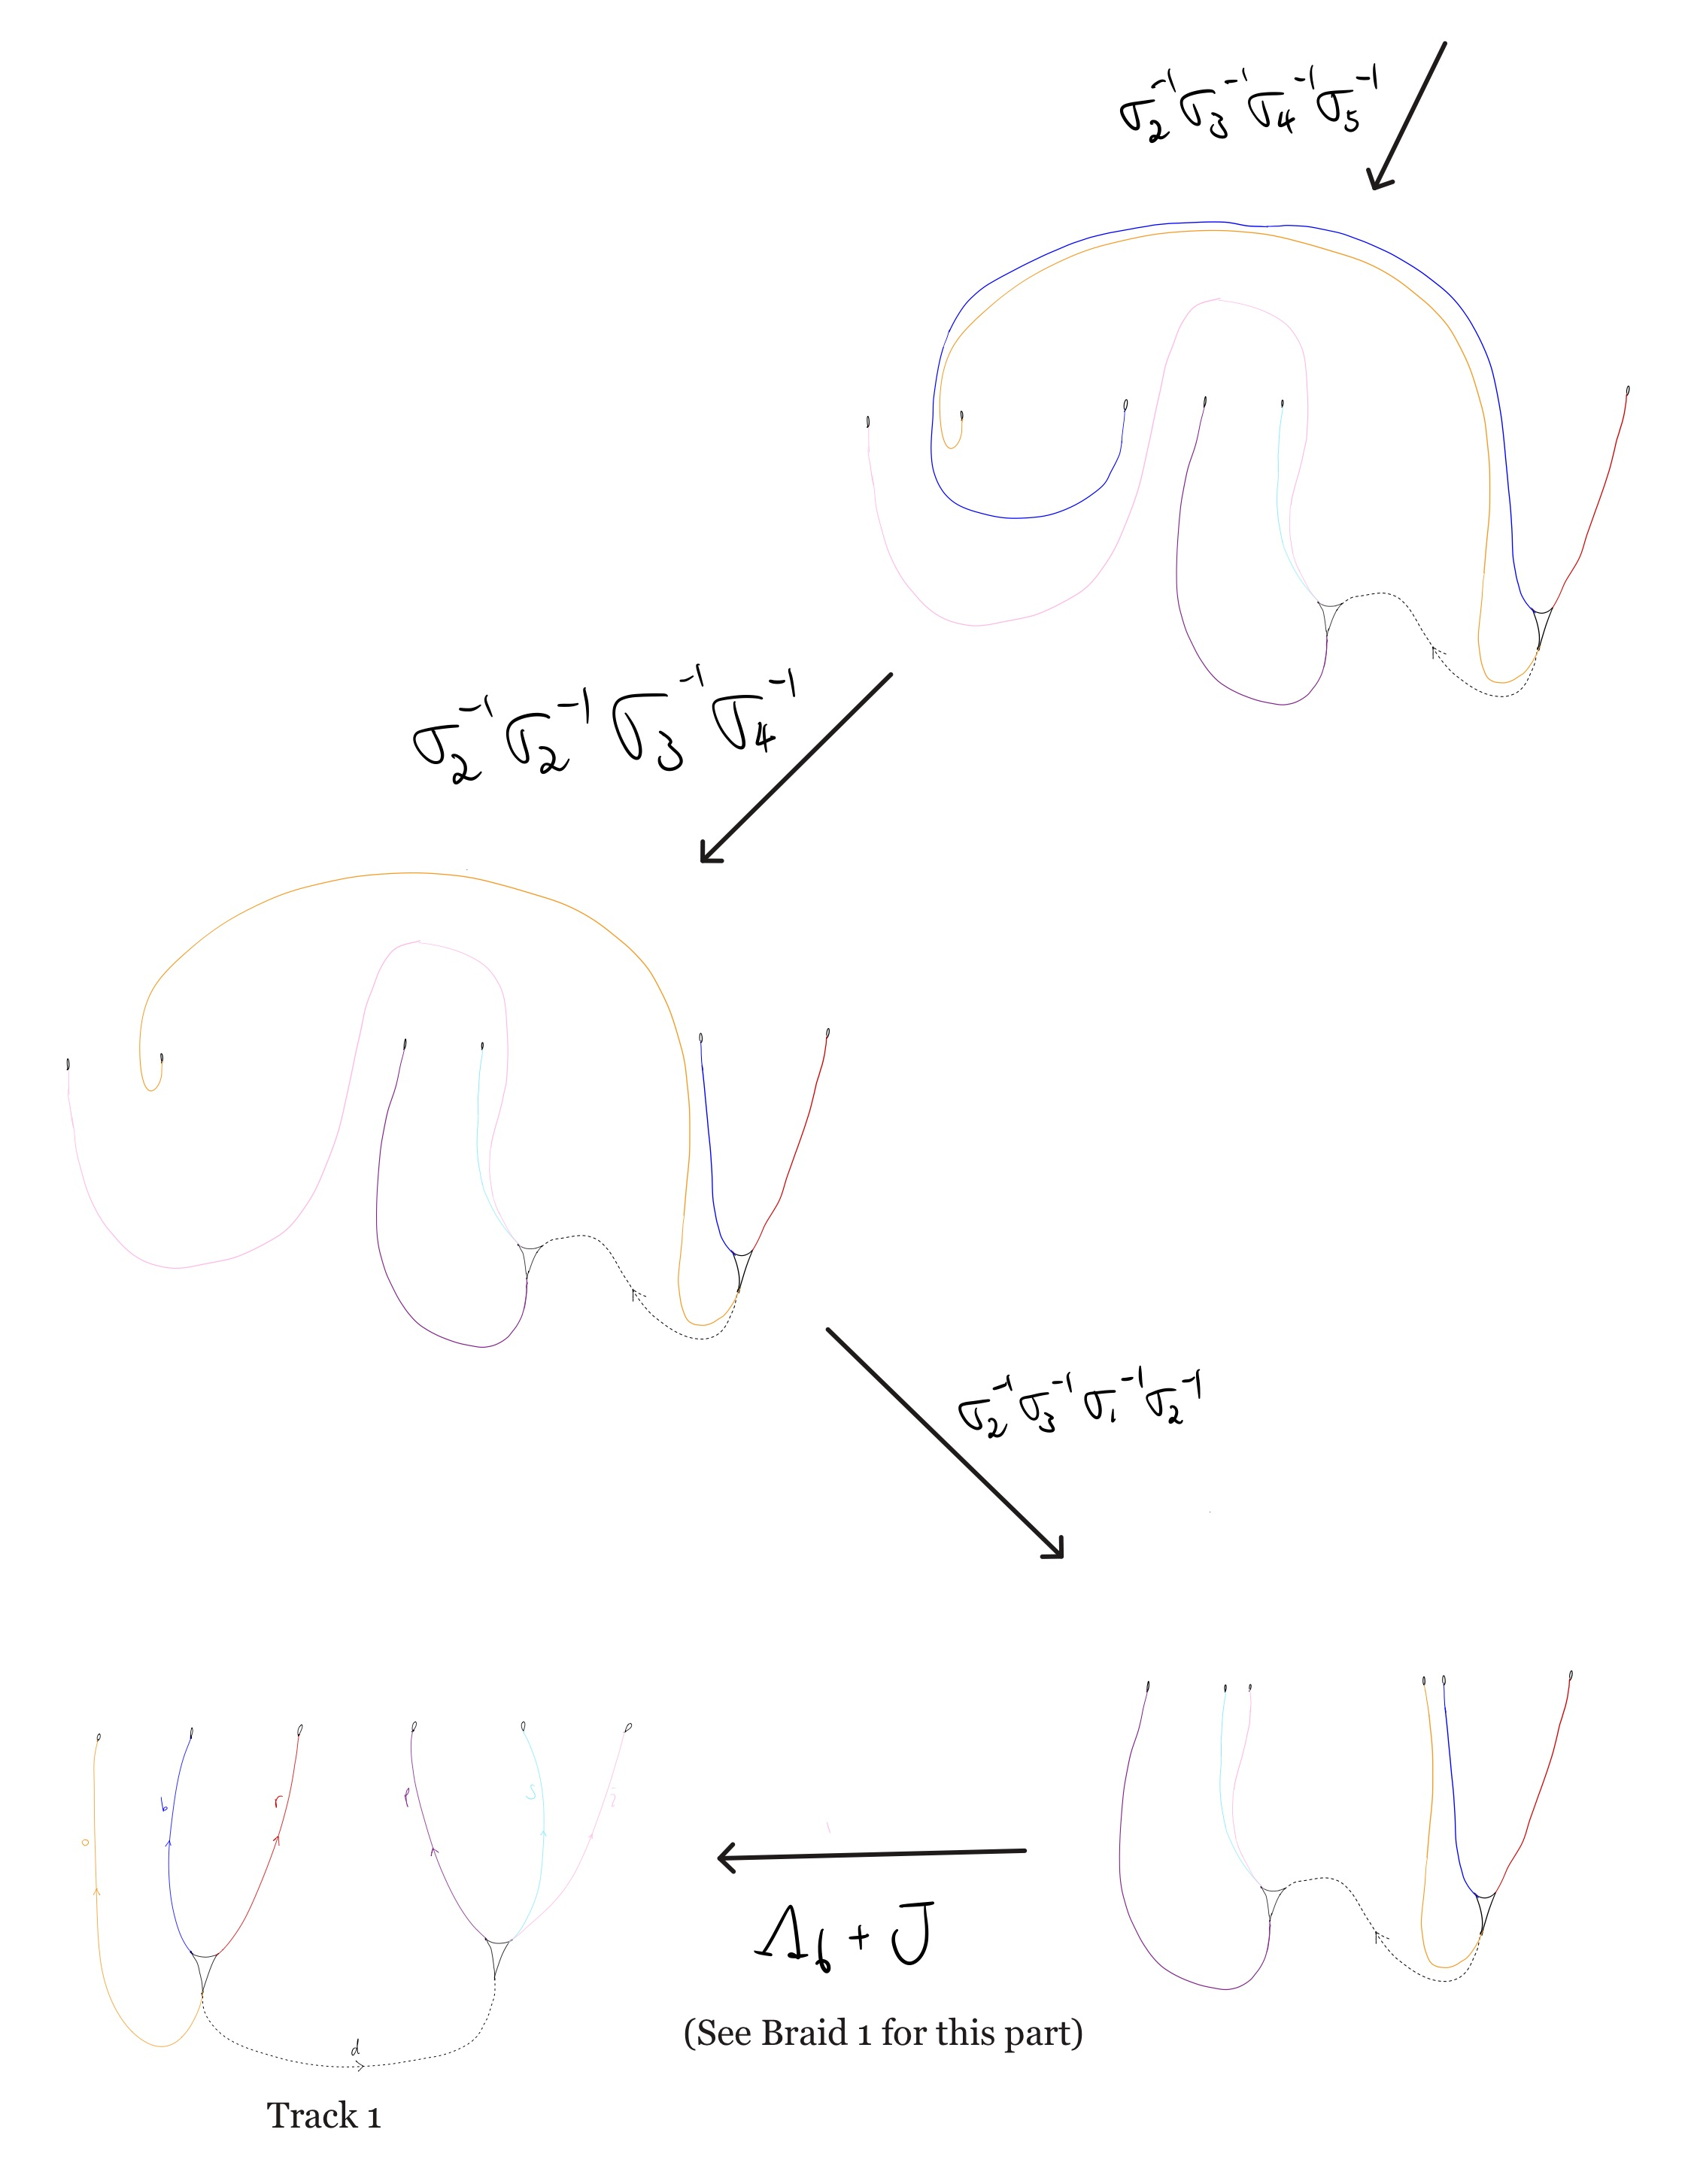
\includegraphics[width=\linewidth, height=0.45\textheight, keepaspectratio]{figures_braid/figures_track_1/Track 1 Braid 3 Magpie-3.jpg}
    \caption{This sequence shows the inverse of the braid $b_3^1$ carries Train Track Candidate Family 3.}
    \label{fig:track1_braid_b1_3}
\end{figure*}

\clearpage

\section{Candidate Family 4 (Bezoar)}\label{sec:track1_bezoar}
Train Track Map Candidate Family 4 of Track 1 is shown in Figure \ref{fig:track1_braid_b1_4_map}. See \ref{Bezoar} for details.

\begin{figure*}[ht]
    \centering
    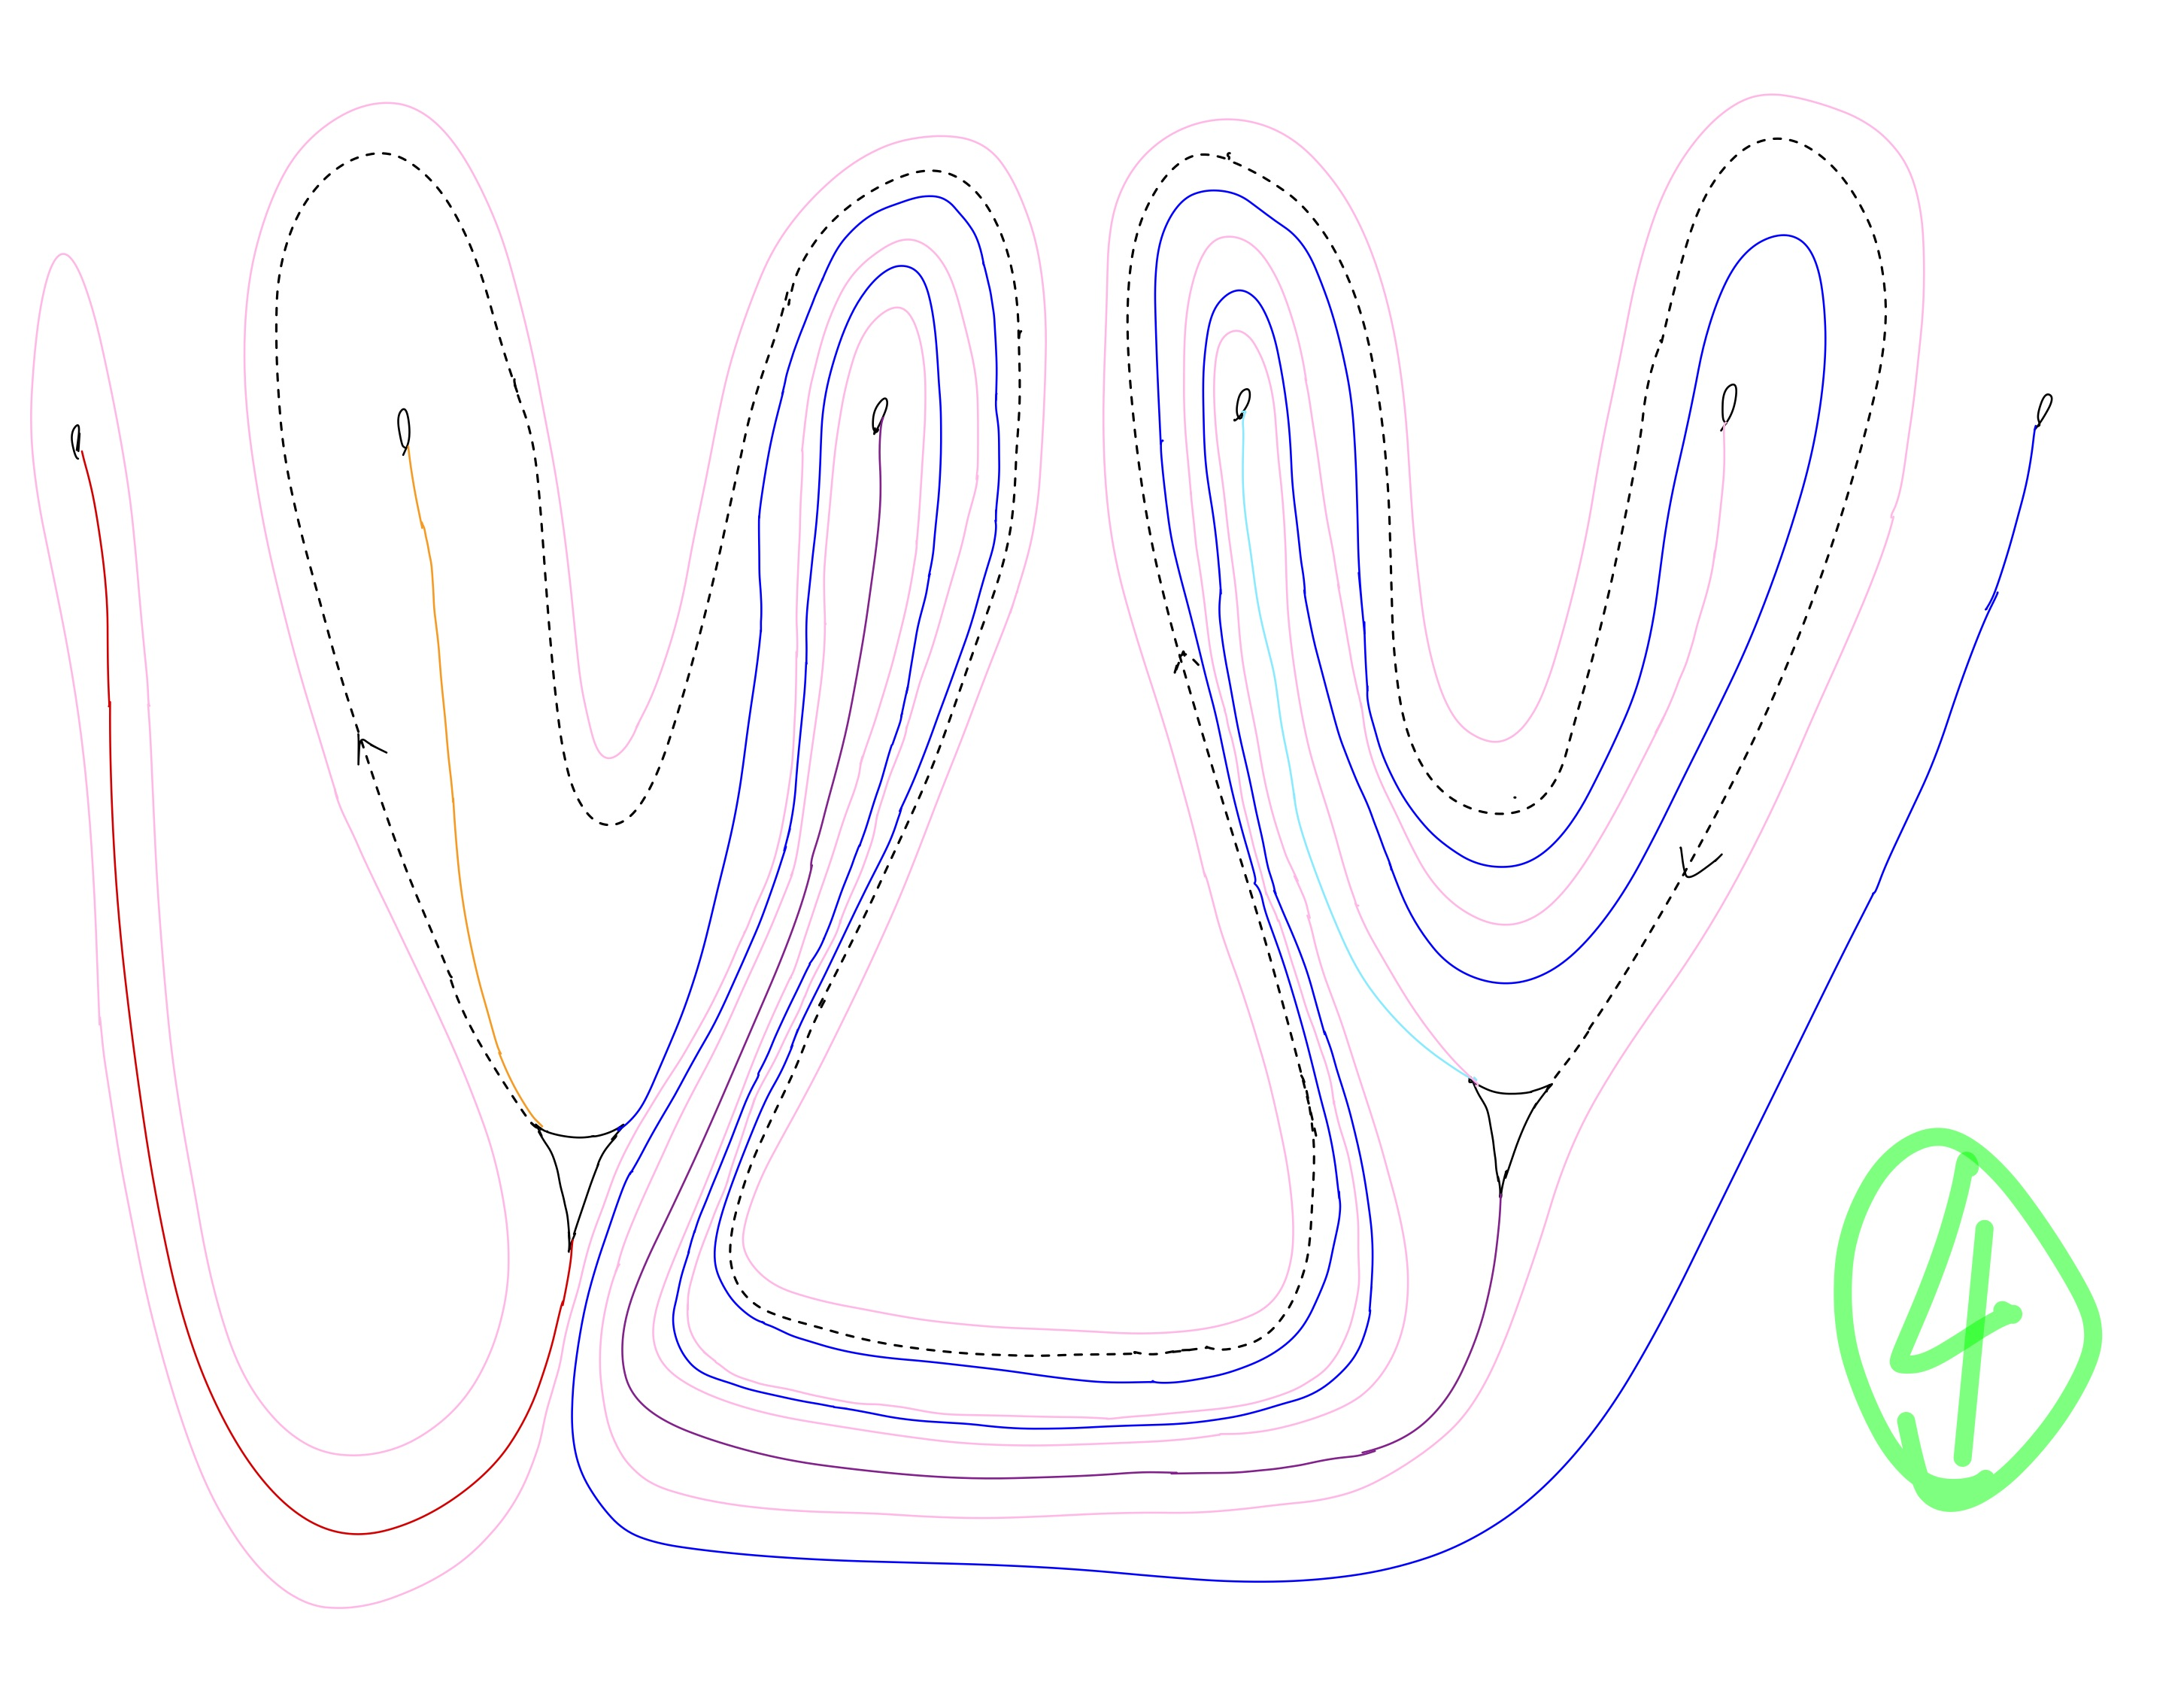
\includegraphics[width=\linewidth, height=0.45\textheight, keepaspectratio]{figures_braid/figures_track_1/Track 1 Braid 4 Bezoar-1.jpg}
    \caption{Train Track Map Candidate Family 4 (Bezoar) of Track 1.}
    \label{fig:track1_braid_b1_4_map}
\end{figure*}

The inverse of the following braid carries this family of train track maps:
\[
b_4^1 = \sigma_{4} \sigma_{3} \sigma_{4} \sigma_{4} \sigma_{3} \sigma_{2} \sigma_{1} \sigma_{4} \sigma_{3} \sigma_{2} \sigma_{5} \sigma_{5} \sigma_{4} \sigma_{3} \sigma_{2}^{-1} \sigma_{1}^{-1} \sigma_{1}^{-1} \sigma_{2}^{-1} \sigma_{4} \sigma_{5} \circ J \circ \Lambda_6
\]

This is shown in Figure \ref{fig:track1_braid_b1_4}.

\begin{figure*}[p]
    \centering
    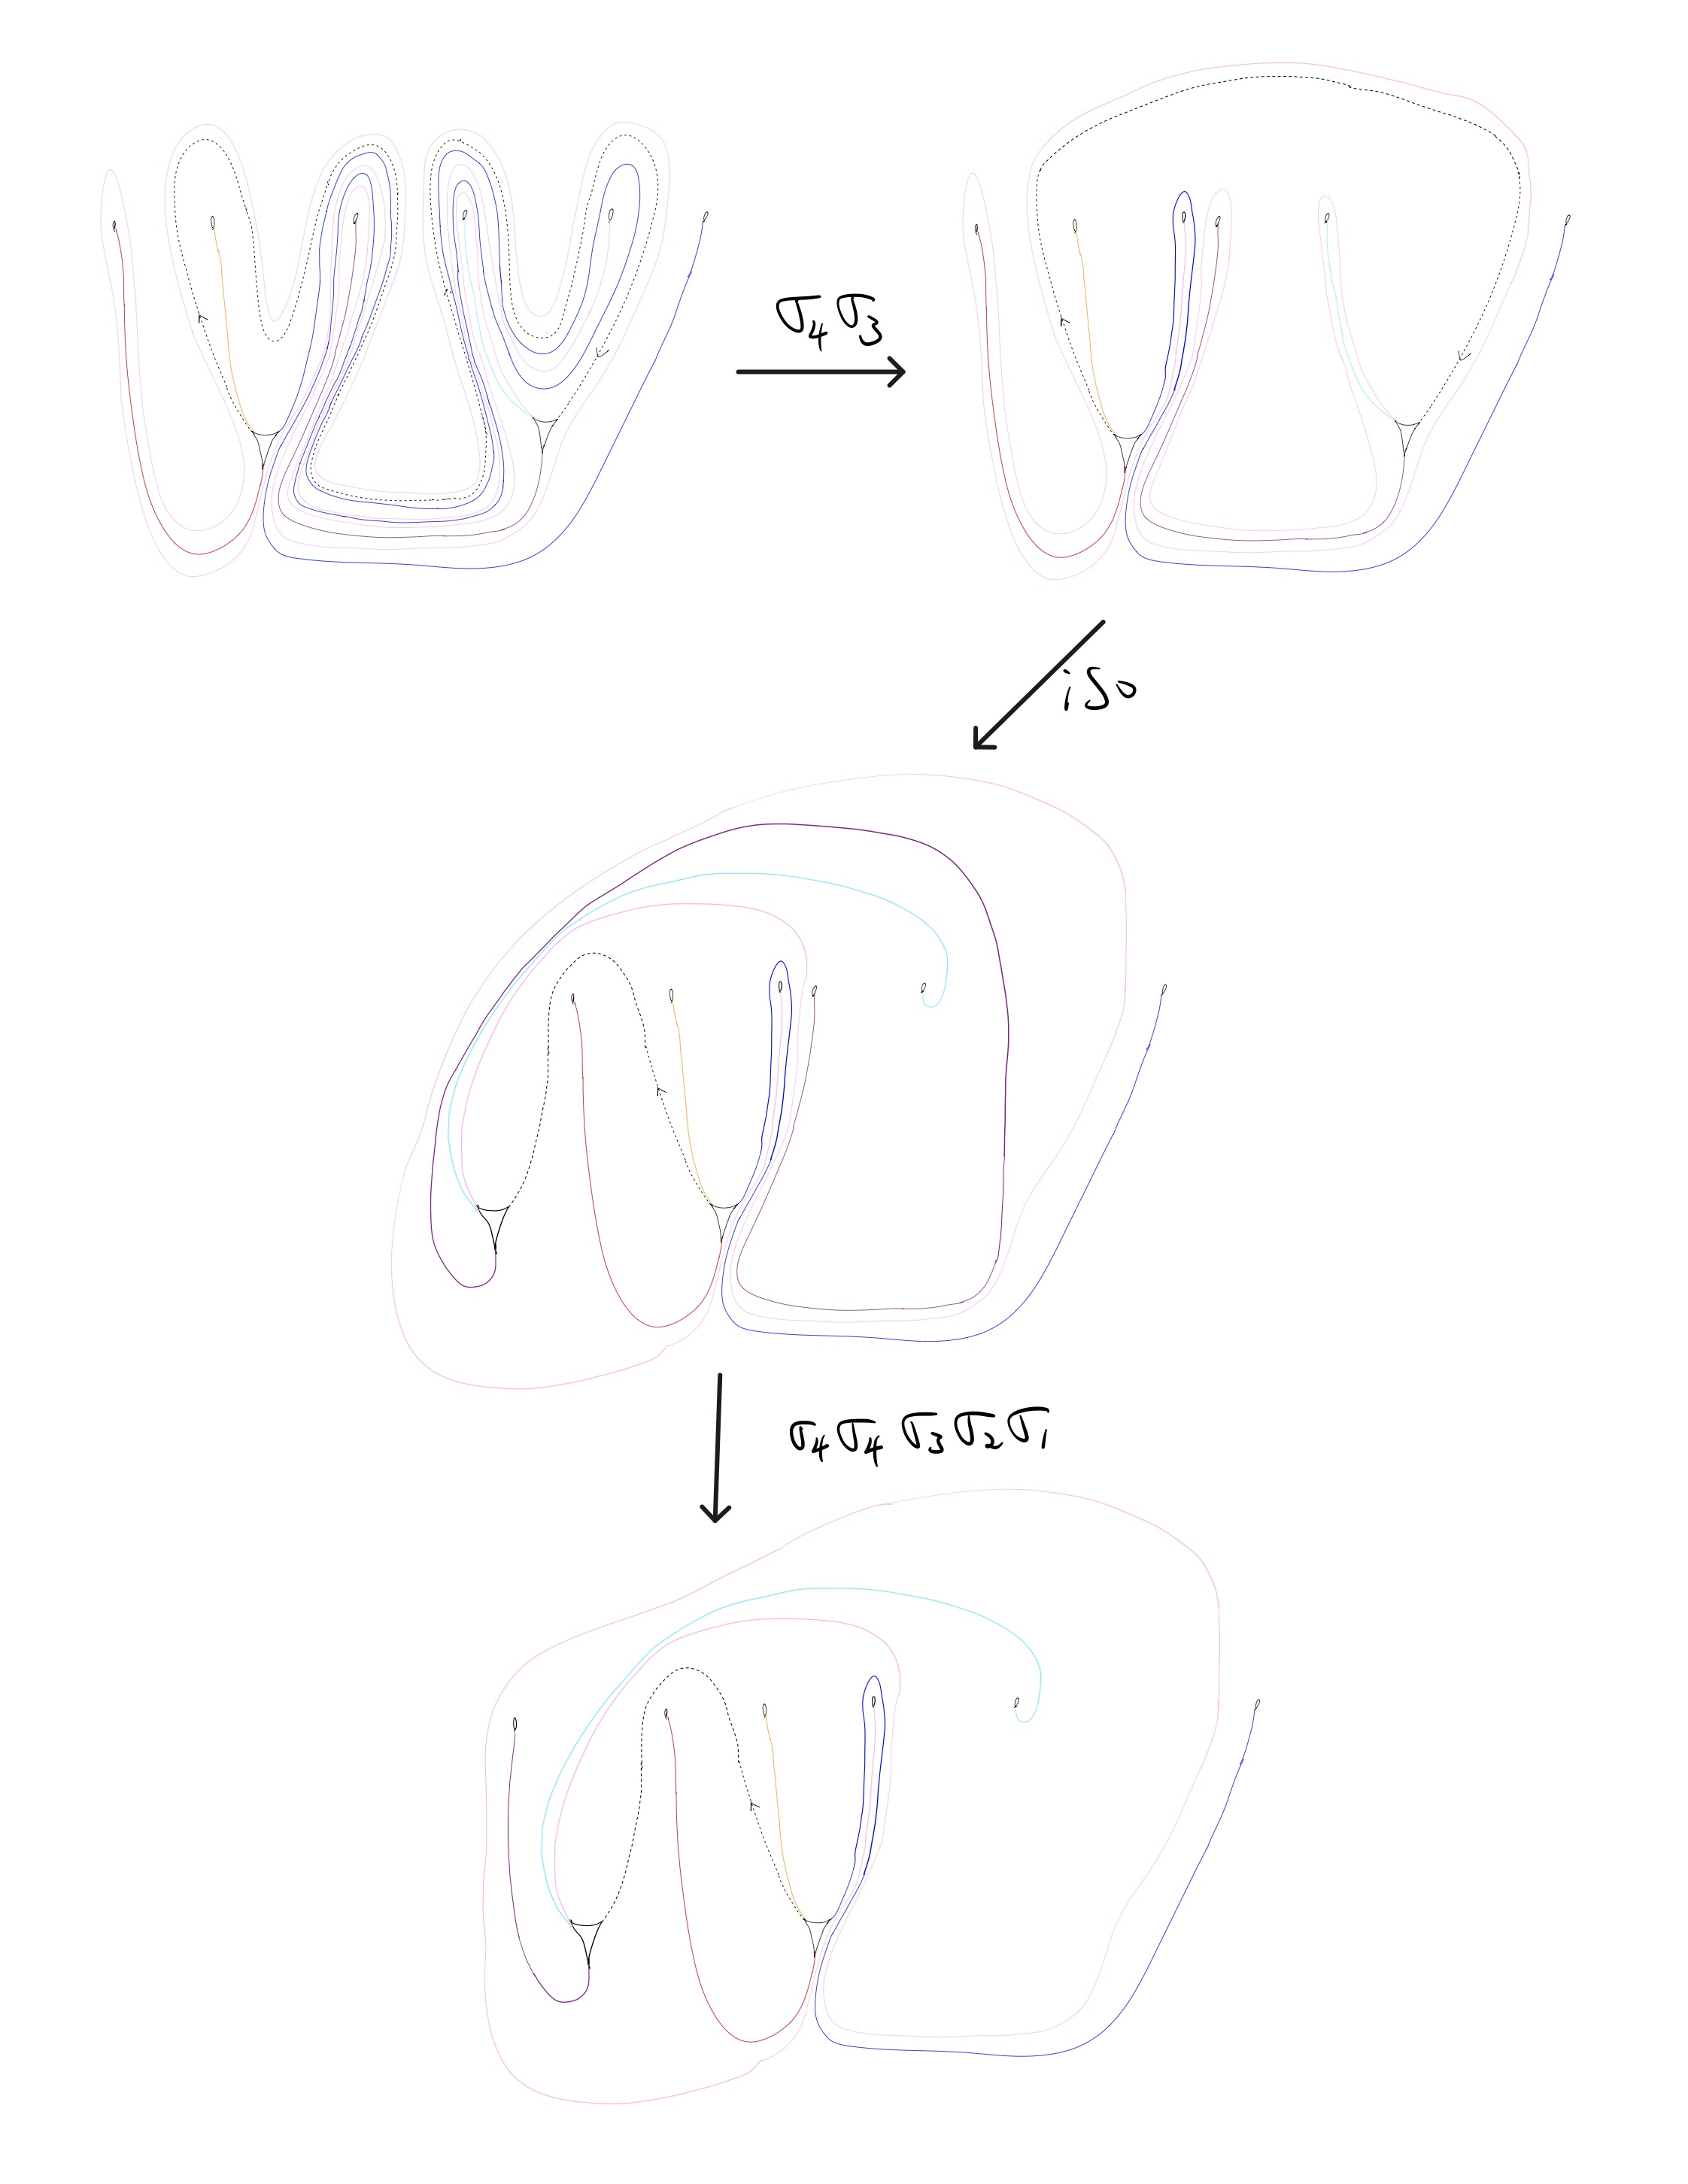
\includegraphics[width=\linewidth, height=0.45\textheight, keepaspectratio]{figures_braid/figures_track_1/Track 1 Braid 4 Bezoar-2.jpg}\\
    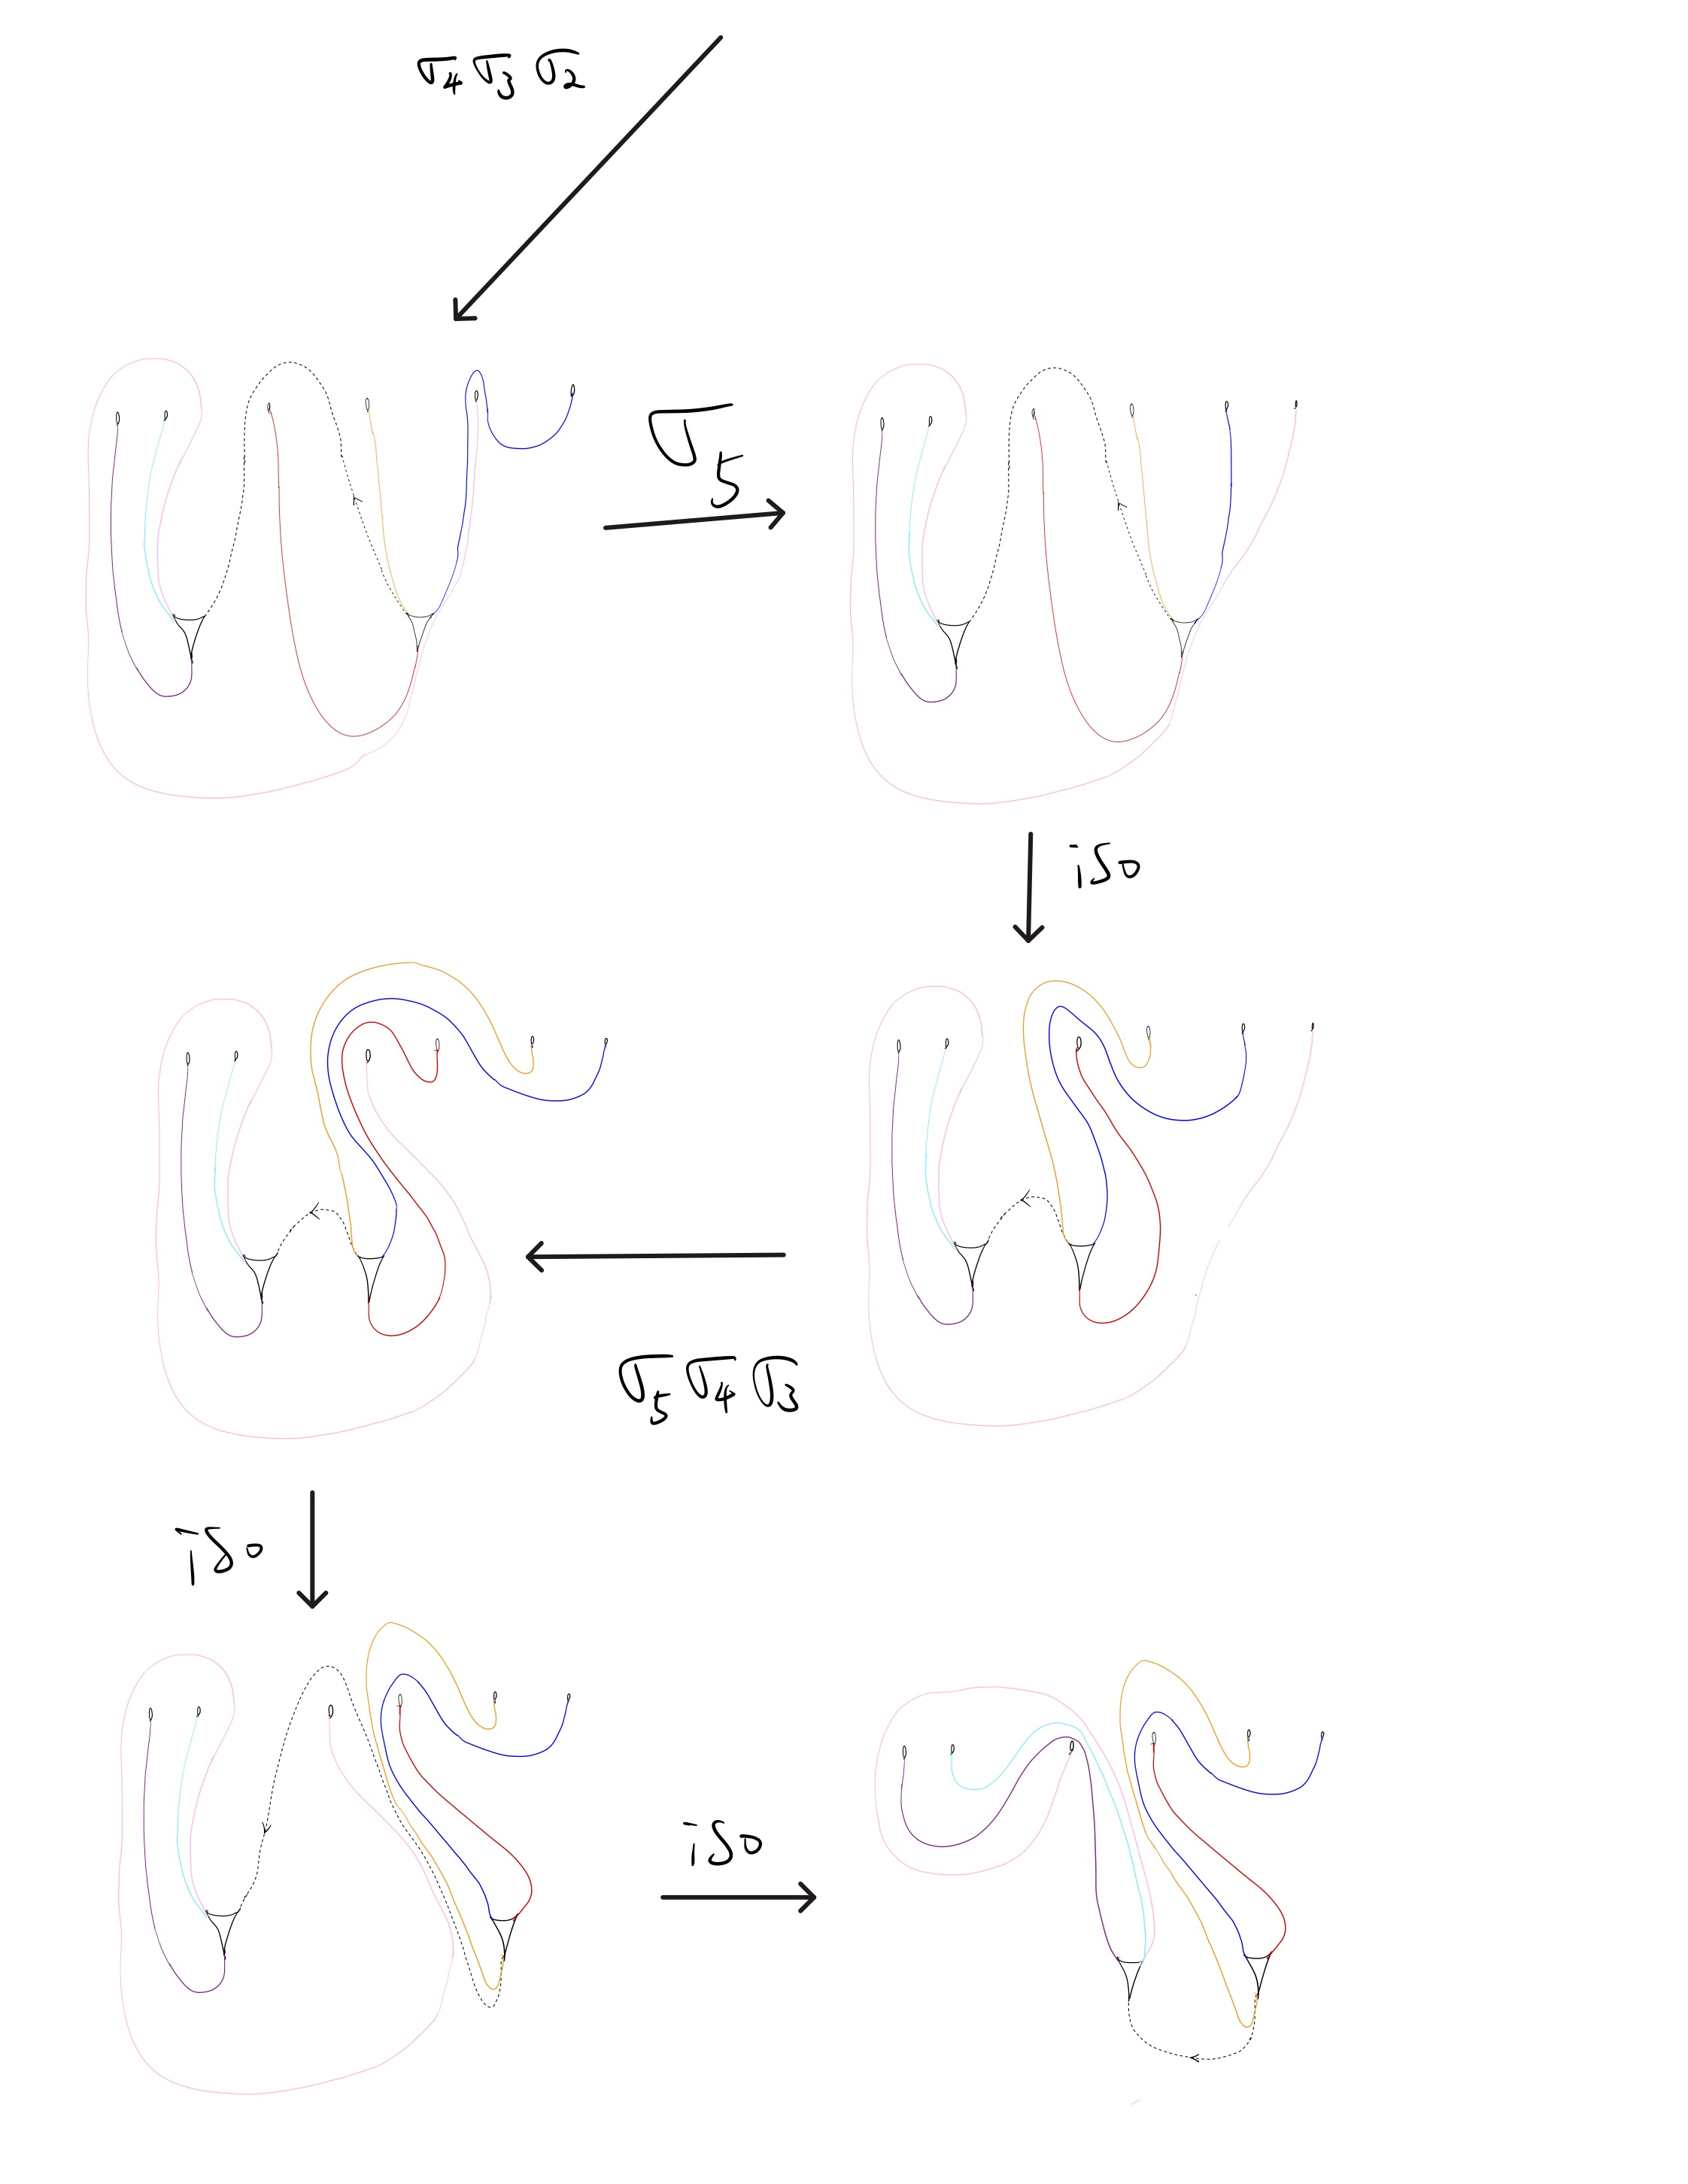
\includegraphics[width=\linewidth, height=0.45\textheight, keepaspectratio]{figures_braid/figures_track_1/Track 1 Braid 4 Bezoar-3.jpg}
    \caption{This sequence shows the inverse of the braid $b_4^1$ carries Train Track Candidate Family 4.}
    \label{fig:track1_braid_b1_4}
\end{figure*}

\clearpage

\section{Candidate Family 5 (Abscond)}\label{sec:track1_abscond_5}
Train Track Map Candidate Family 5 of Track 1 is shown in Figure \ref{fig:track1_braid_b1_5_map}. See \ref{Abscond} for details.

\begin{figure*}[ht]
    \centering
    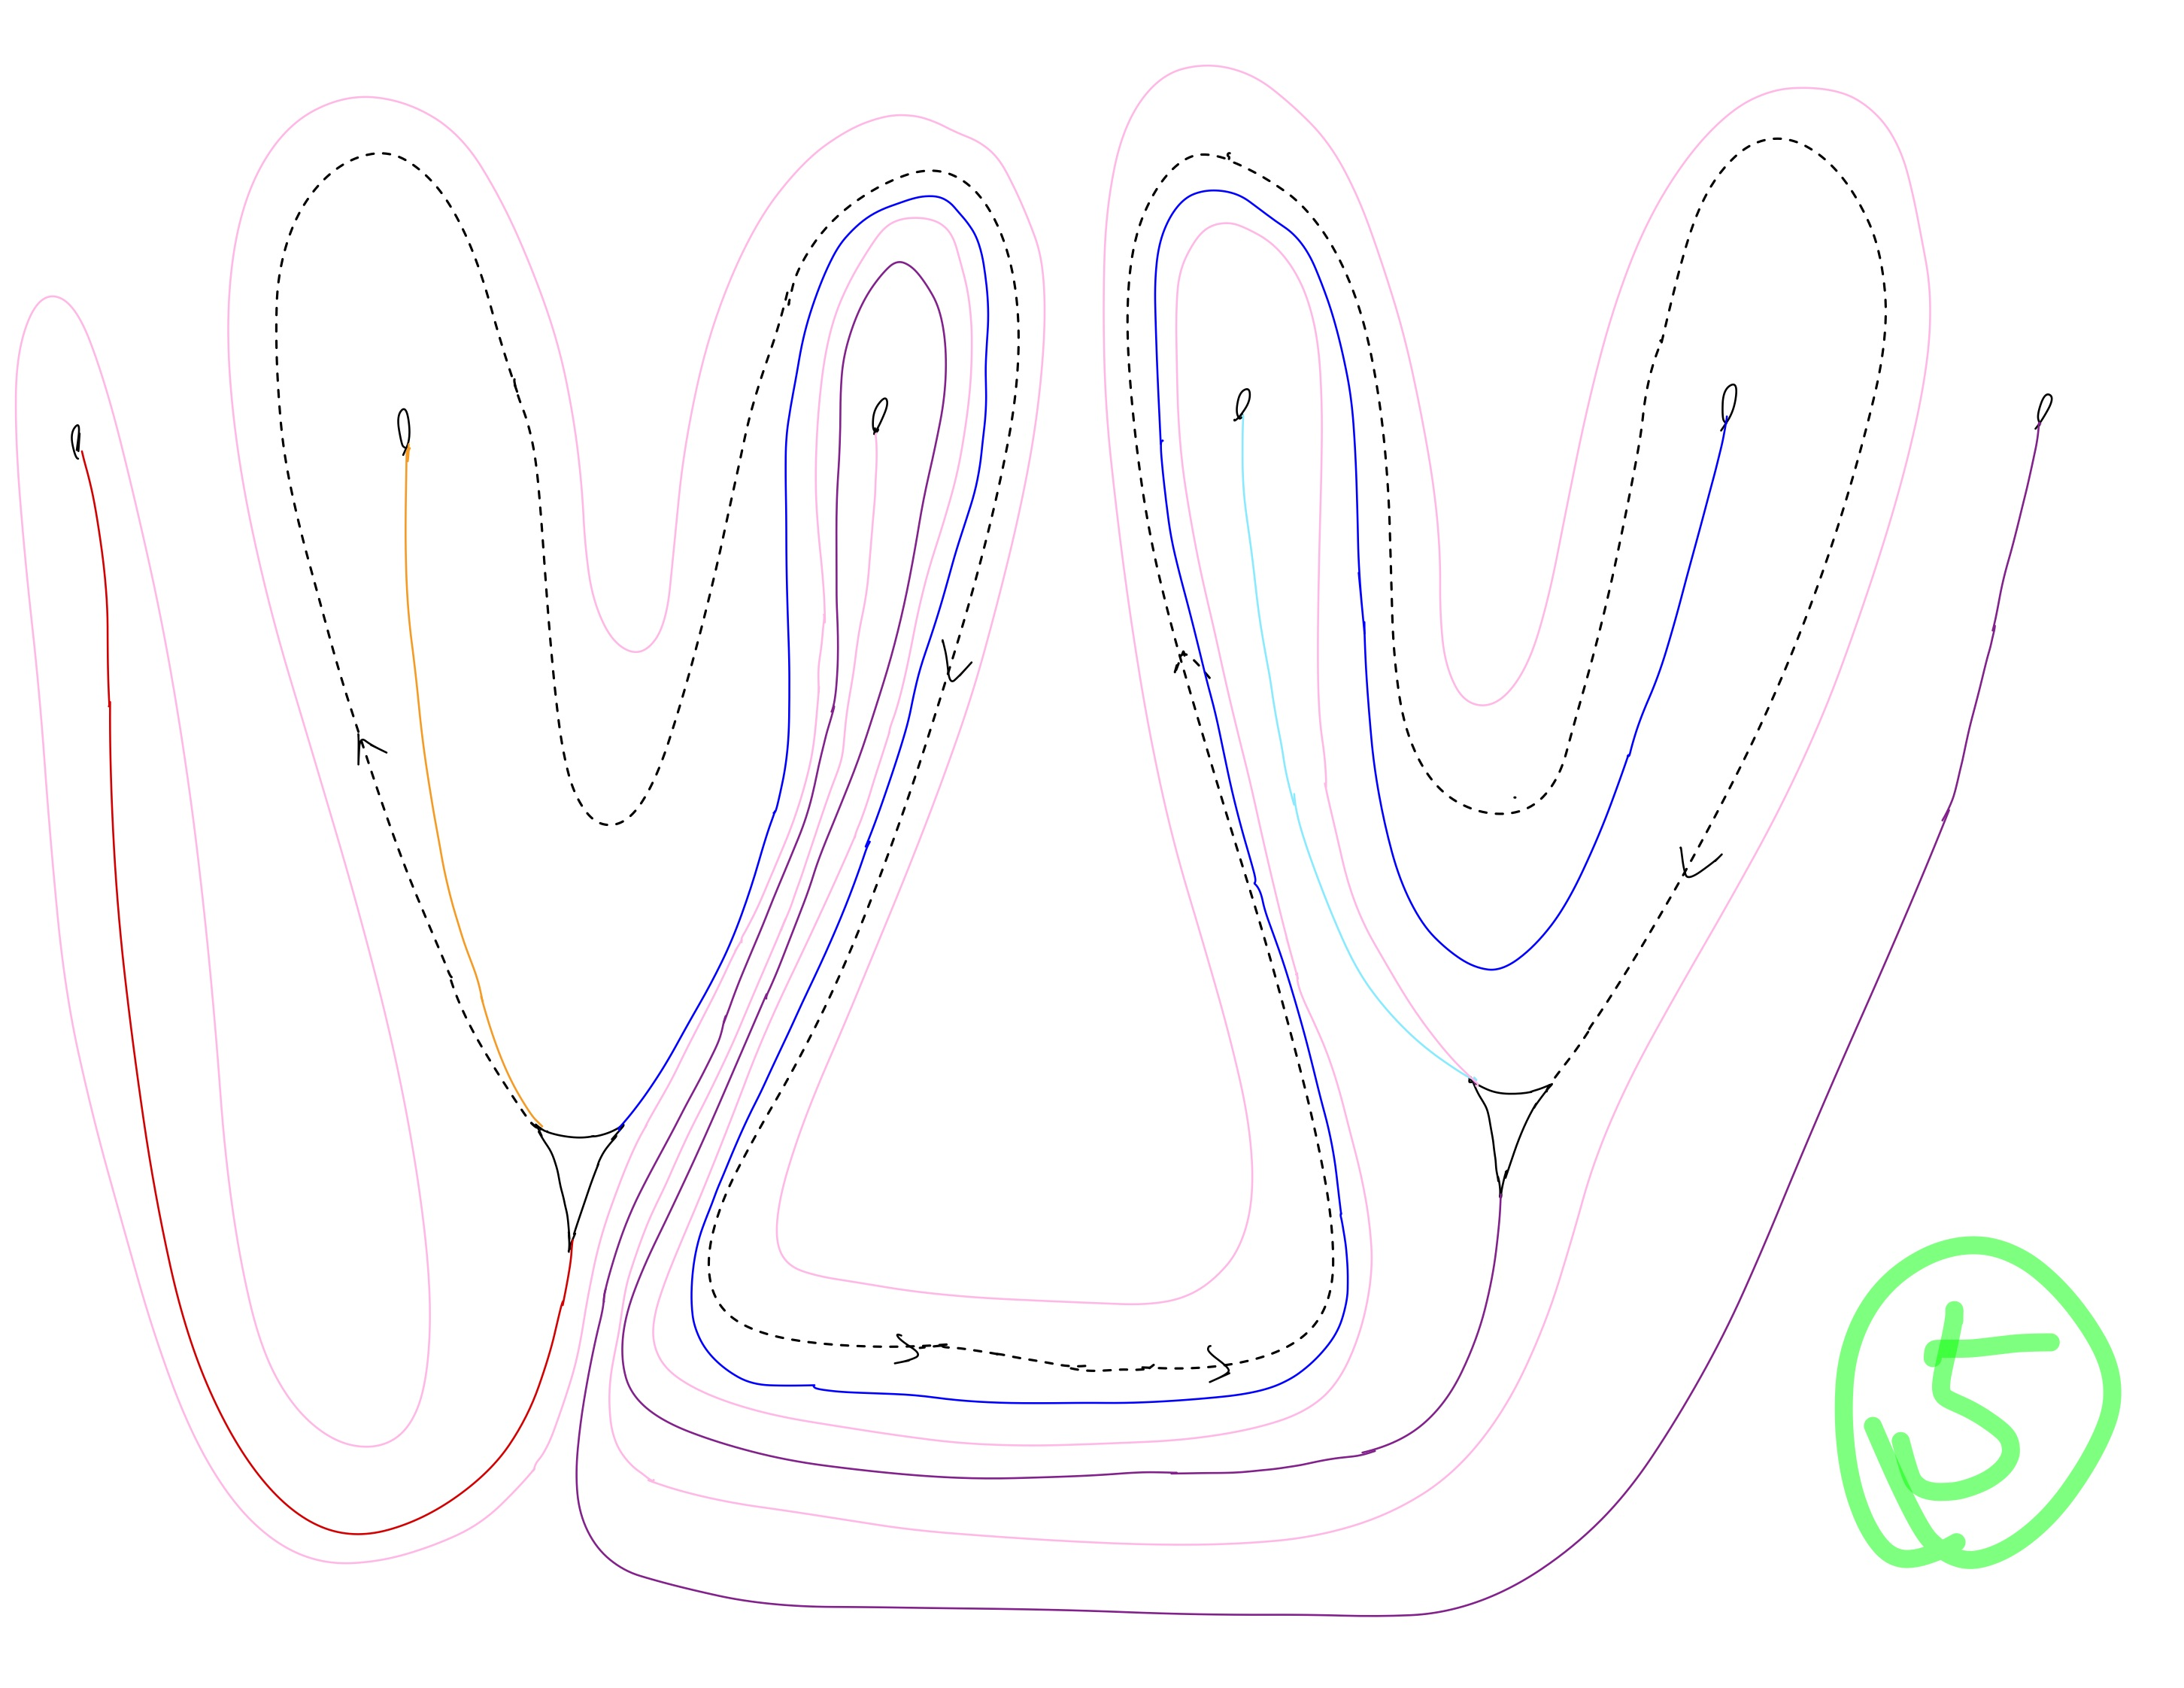
\includegraphics[width=\linewidth, height=0.45\textheight, keepaspectratio]{figures_braid/figures_track_1/Track 1 Braid 5 Abscond-1.jpg}
    \caption{Train Track Map Candidate Family 5 (Abscond) of Track 1.}
    \label{fig:track1_braid_b1_5_map}
\end{figure*}

The inverse of the following braid carries this family of train track maps:
\[
b_5^1 = \sigma_{4} \sigma_{3} \sigma_{4} \sigma_{4} \sigma_{3} \sigma_{2} \sigma_{1} \sigma_{1} \sigma_{2} \sigma_{3} \sigma_{1}^{-1} \sigma_{2}^{-1} \sigma_{1}^{-1} \sigma_{1}^{-1} \sigma_{5} \sigma_{4} \sigma_{5}
\]

This is shown in Figure \ref{fig:track1_braid_b1_5}.

\begin{figure*}[p]
    \centering
    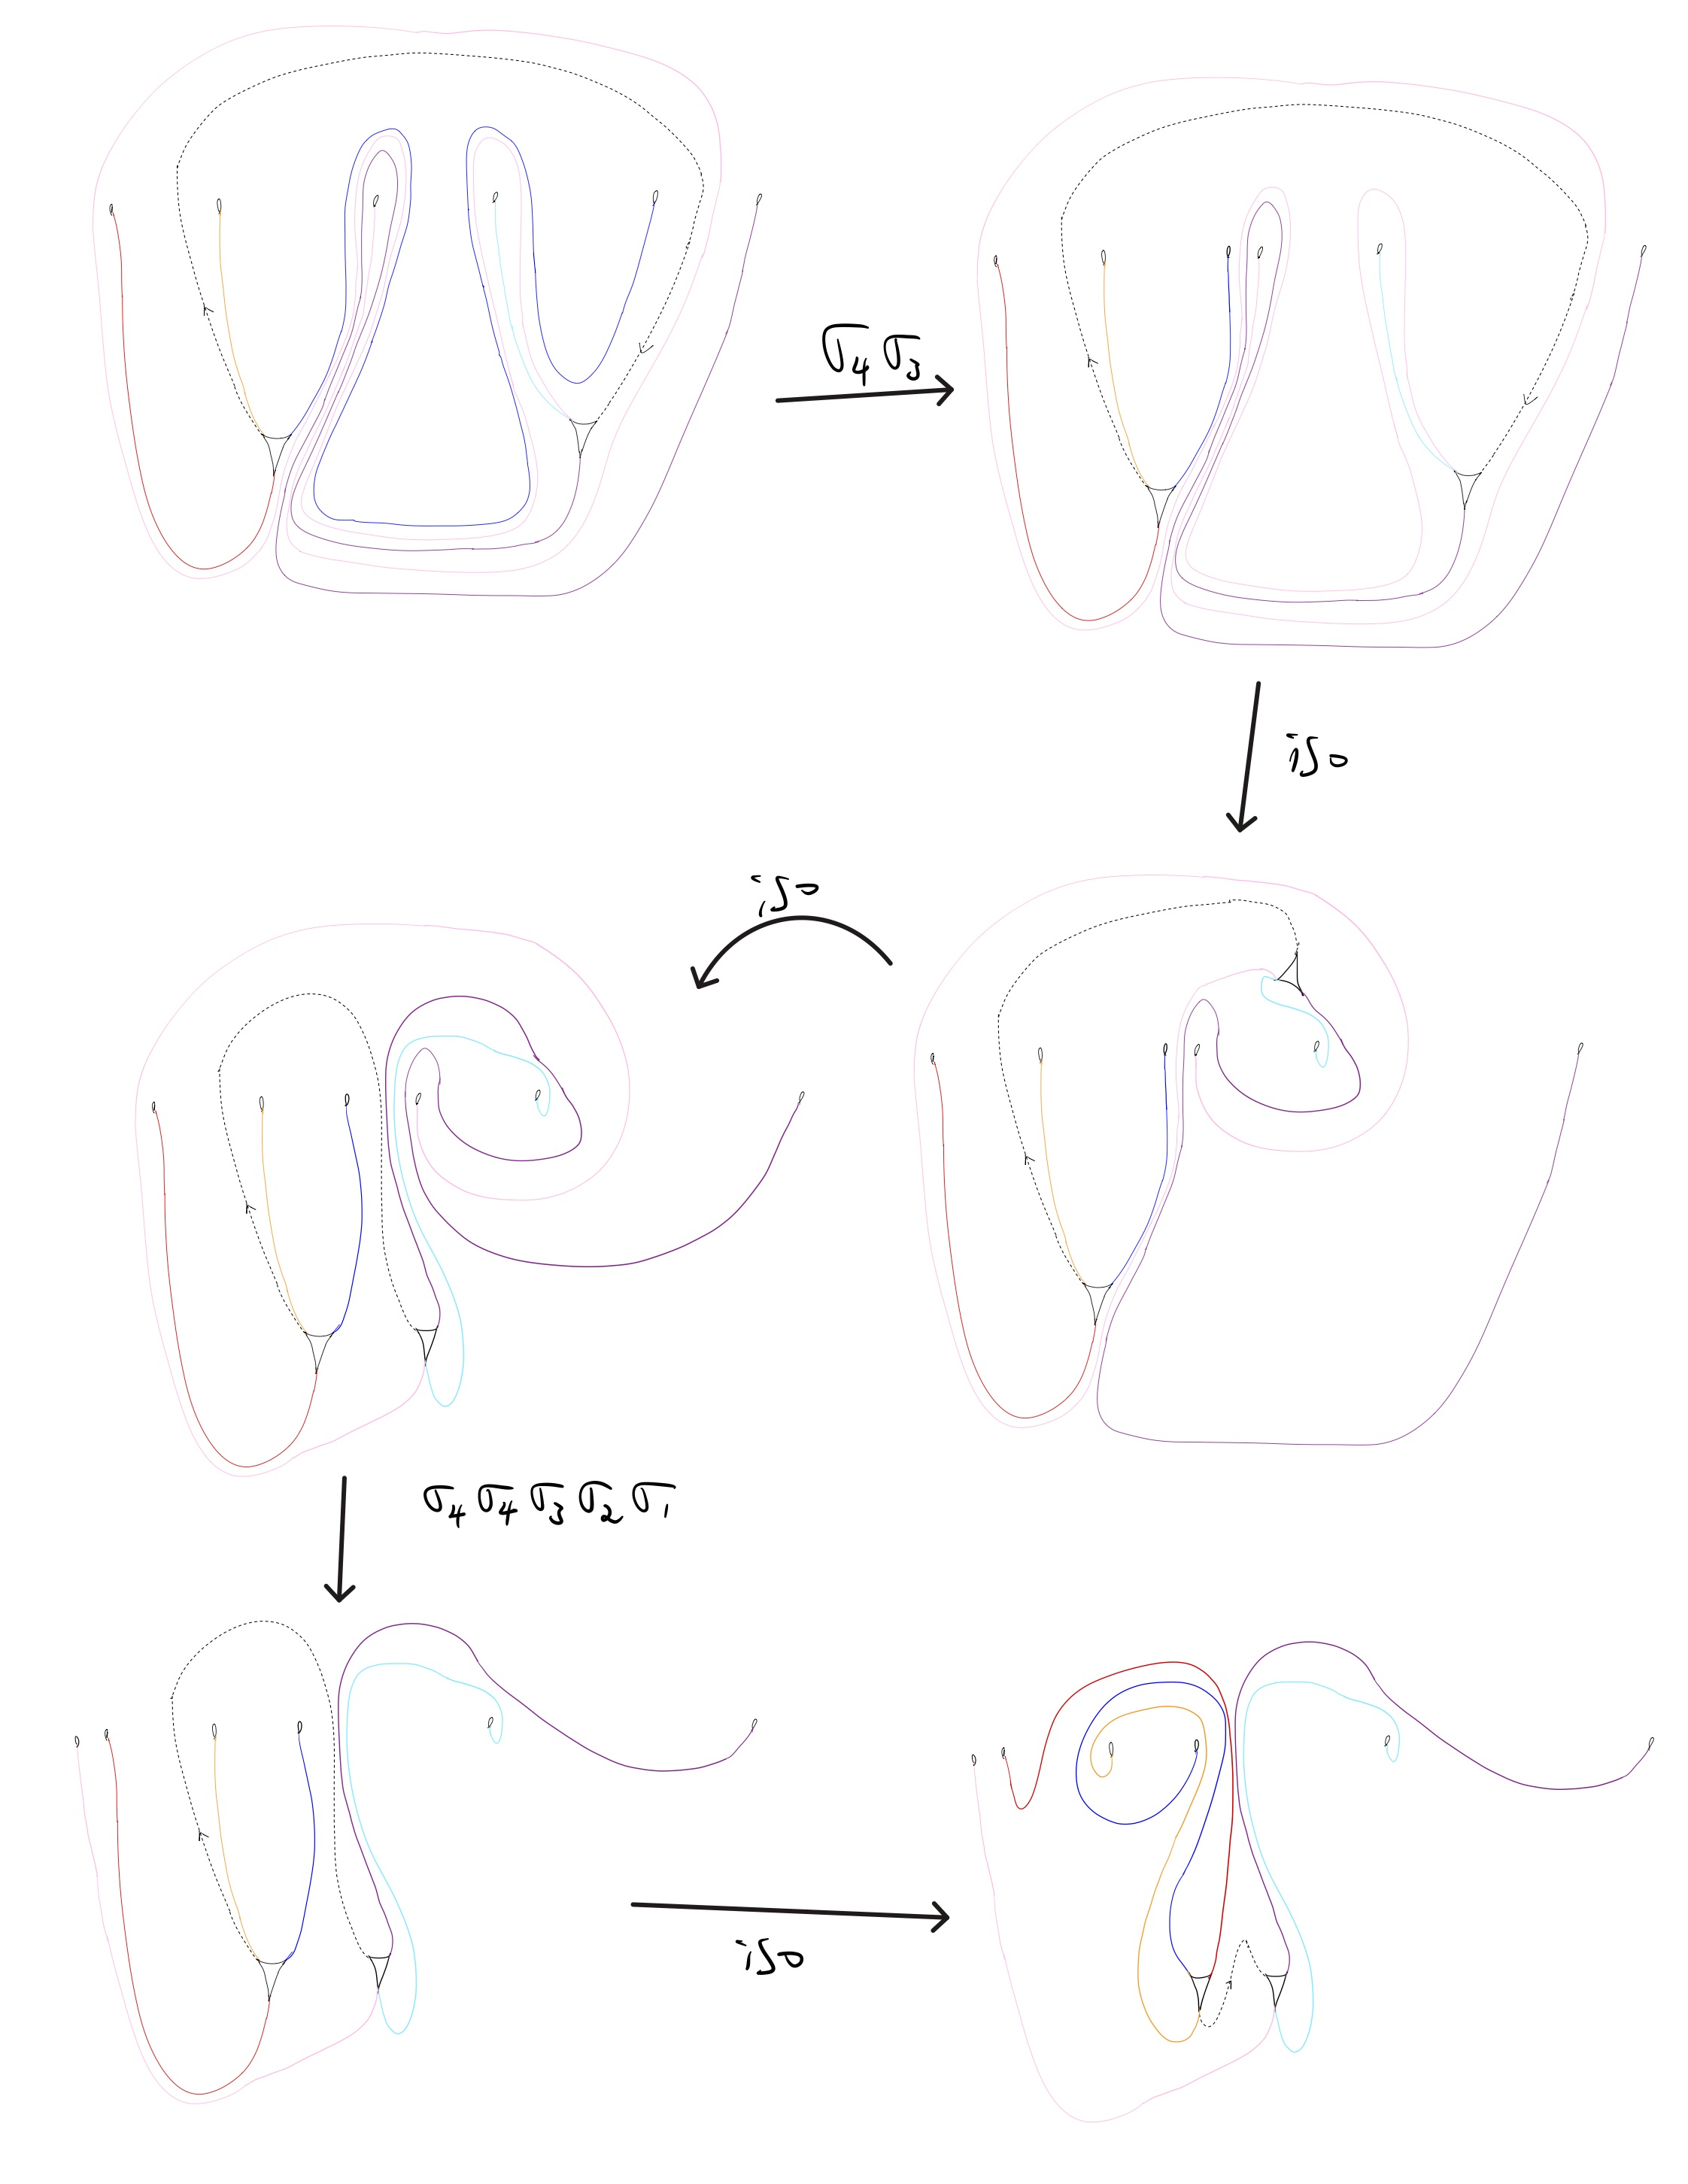
\includegraphics[width=\linewidth, height=0.45\textheight, keepaspectratio]{figures_braid/figures_track_1/Track 1 Braid 5 Abscond-2.jpg}\\
    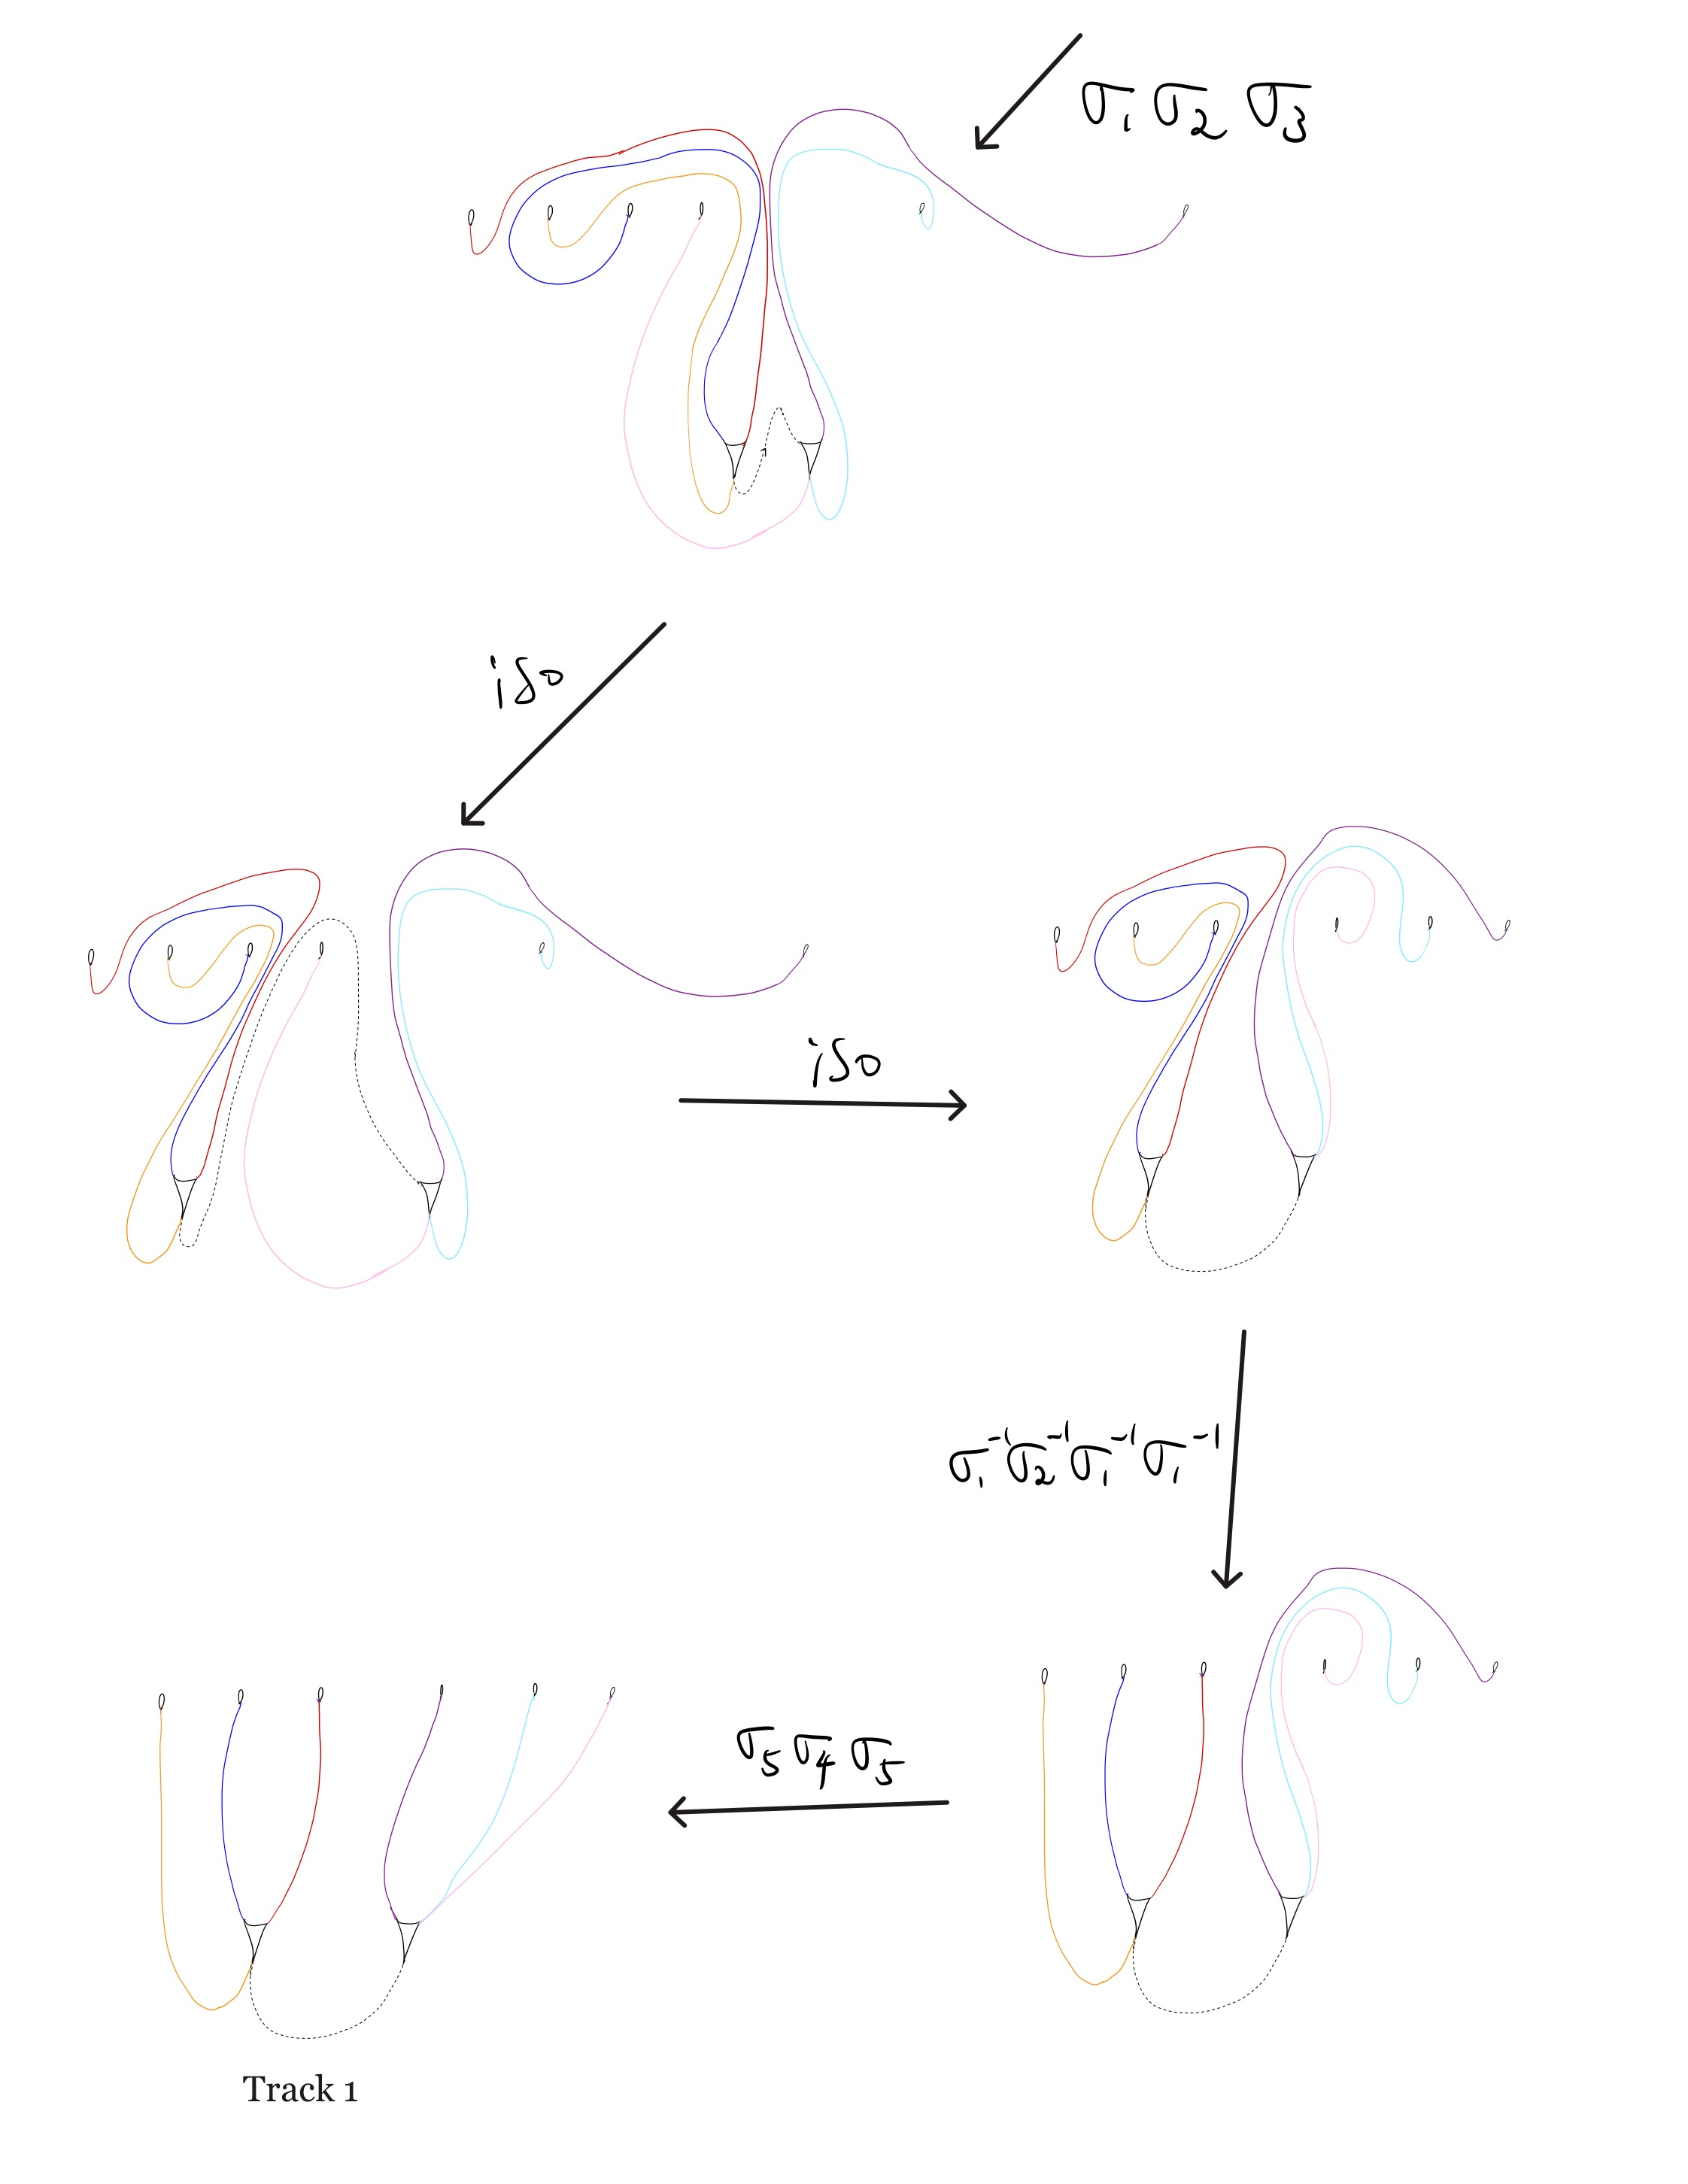
\includegraphics[width=\linewidth, height=0.45\textheight, keepaspectratio]{figures_braid/figures_track_1/Track 1 Braid 5 Abscond-3.jpg}
    \caption{This sequence shows the inverse of the braid $b_5^1$ carries Train Track Candidate Family 5.}
    \label{fig:track1_braid_b1_5}
\end{figure*}

\clearpage

\section{Candidate Family 6 (Abscond)}\label{sec:track1_abscond_6}
Train Track Map Candidate Family 6 of Track 1 is shown in Figure \ref{fig:track1_braid_b1_6_map}. See \ref{Abscond} for details.

\begin{figure*}[ht]
    \centering
    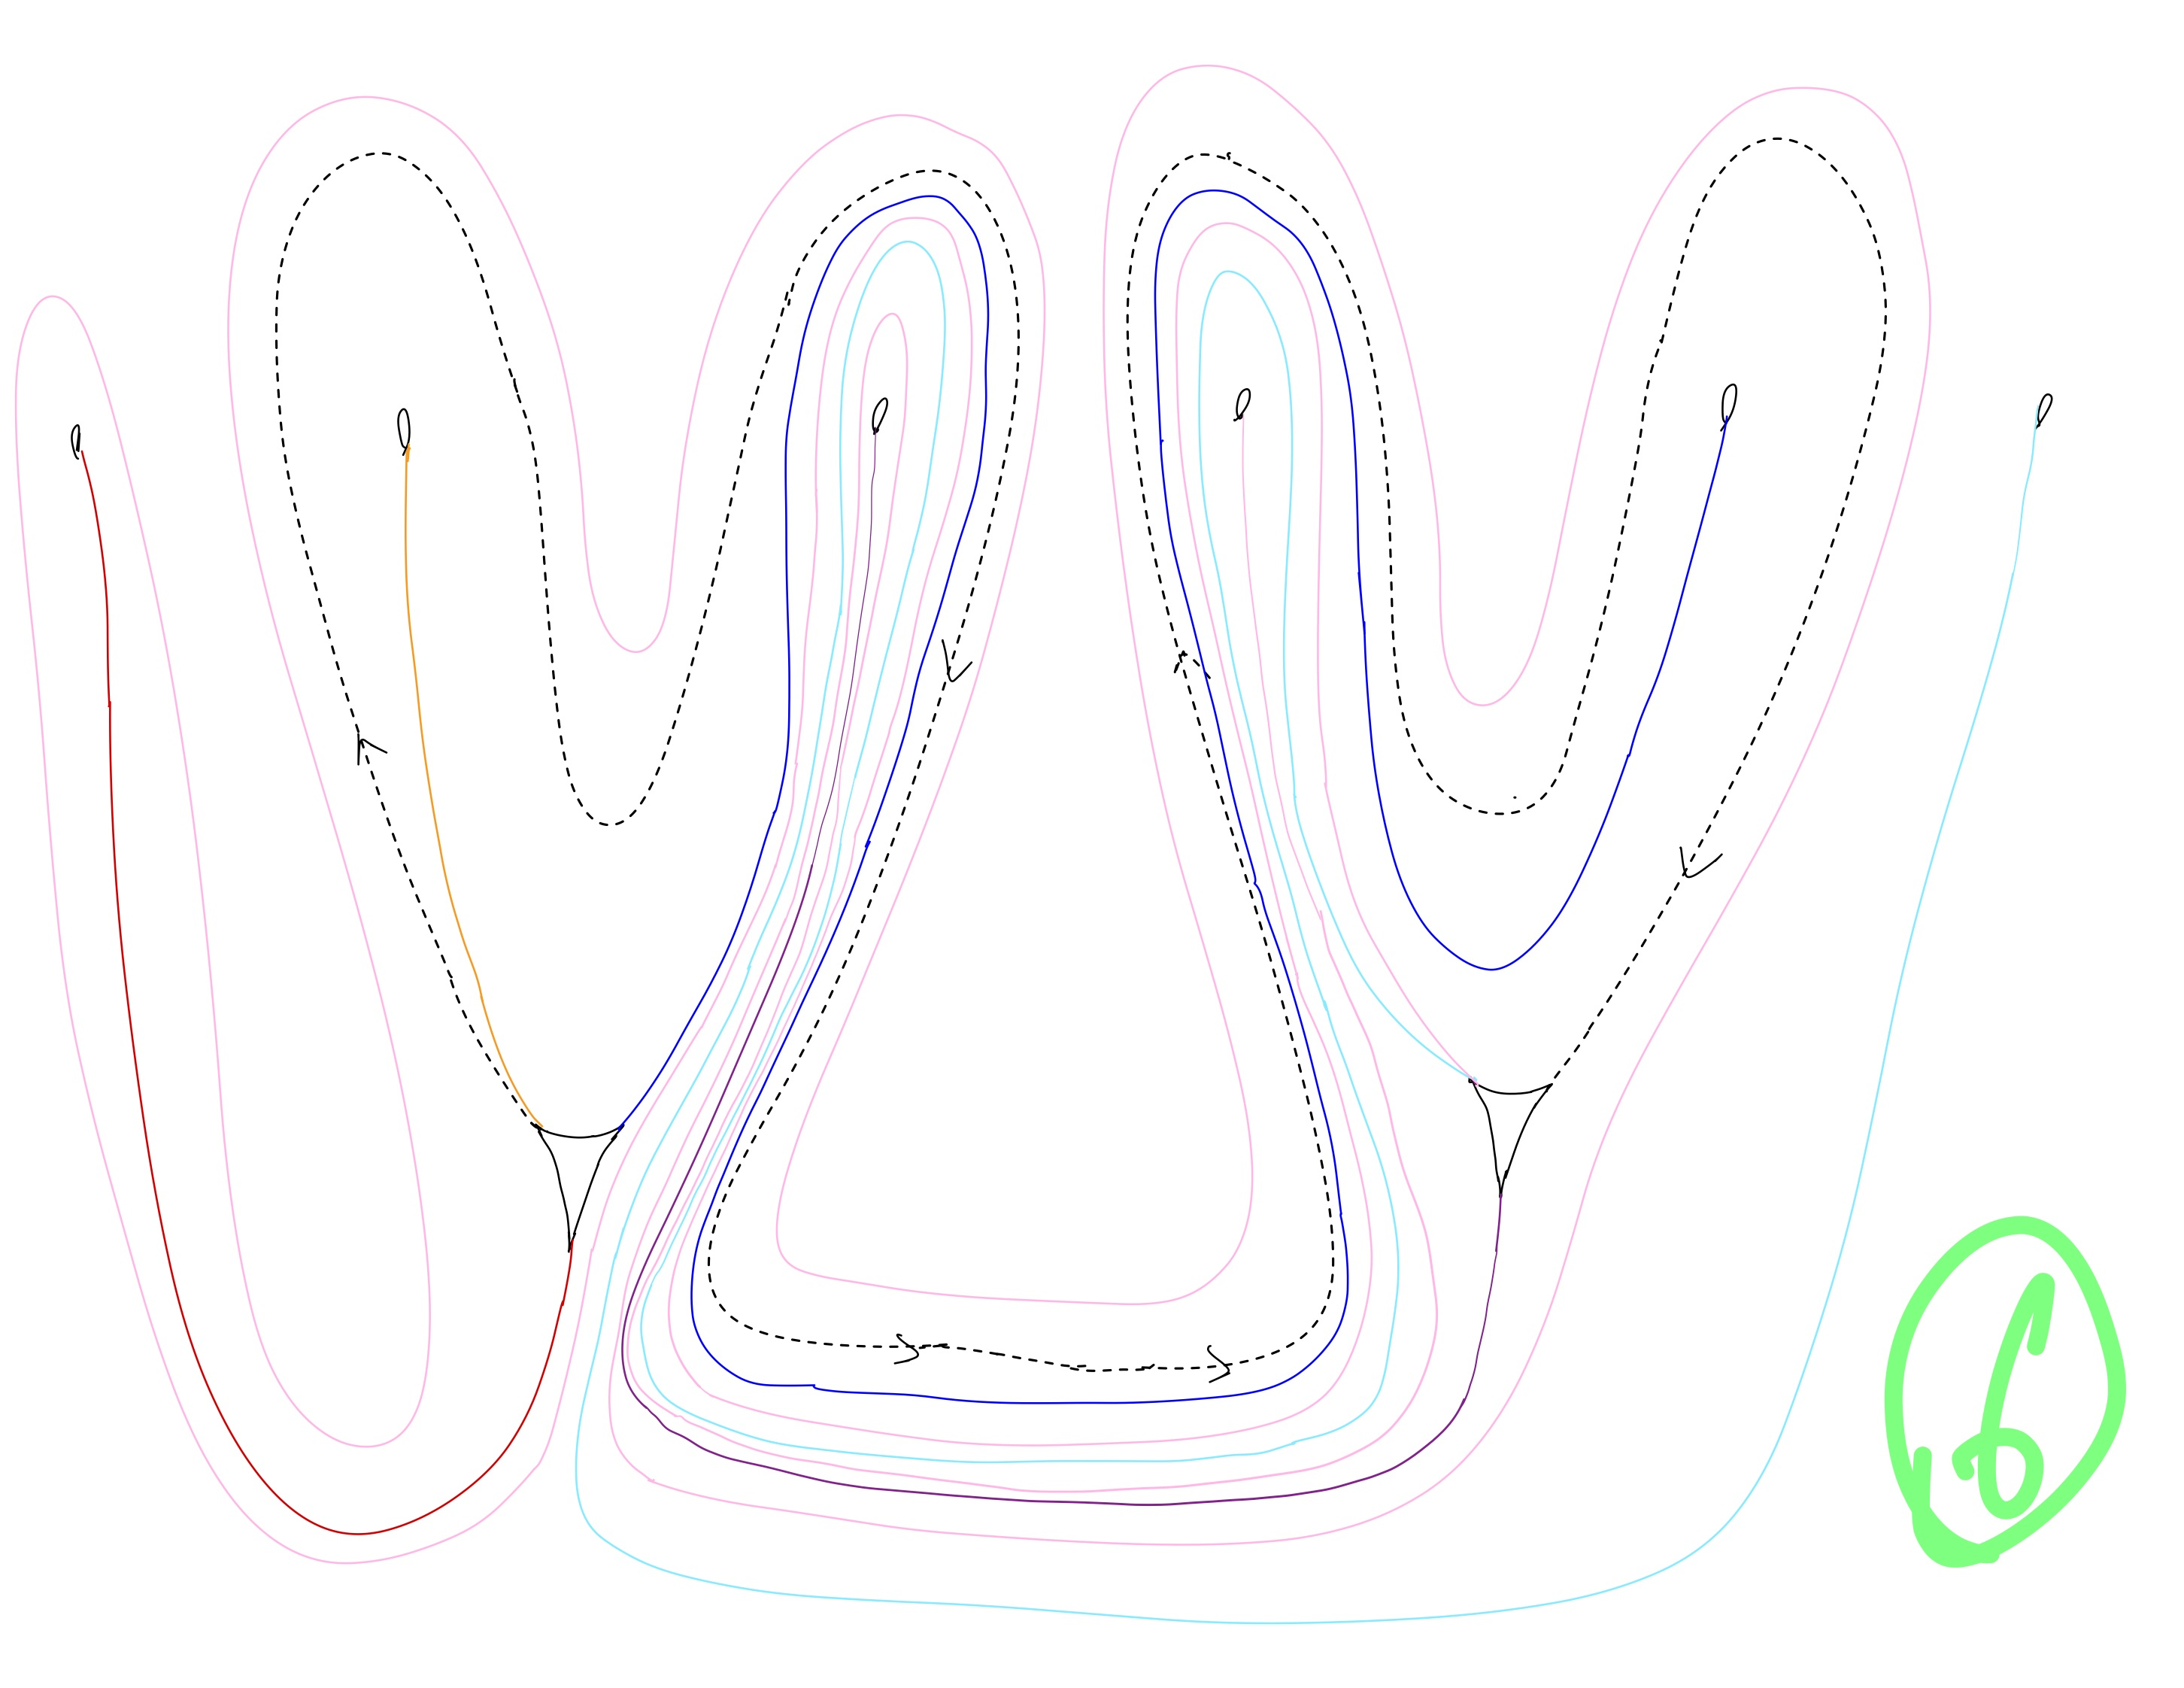
\includegraphics[width=\linewidth, height=0.45\textheight, keepaspectratio]{figures_braid/figures_track_1/Track 1 Braid 6 Abscond-1.jpg}
    \caption{Train Track Map Candidate Family 6 (Abscond) of Track 1.}
    \label{fig:track1_braid_b1_6_map}
\end{figure*}

The inverse of the following braid carries this family of train track maps:
\[
b_6^1 = \sigma_{4} \sigma_{3} \sigma_{4}^k \sigma_{4} \sigma_{4} \sigma_{3} \sigma_{2} \sigma_{1} \sigma_{4} \sigma_{3} \sigma_{2} \sigma_{5} \sigma_{4} \sigma_{3} \sigma_{1} \sigma_{2} \sigma_{1} \sigma_{3} \sigma_{4} \sigma_{5} \sigma_{5} \sigma_{4} \sigma_{3} \sigma_{1}^{-1} \sigma_{4} \sigma_{5} \circ J \circ \Lambda_6
\]
where $k \geq 1$ ($k \in \mathbb{Z}$) is the twisting parameter. This is shown in Figure \ref{fig:track1_braid_b1_6}.

\begin{figure*}[p]
    \centering
    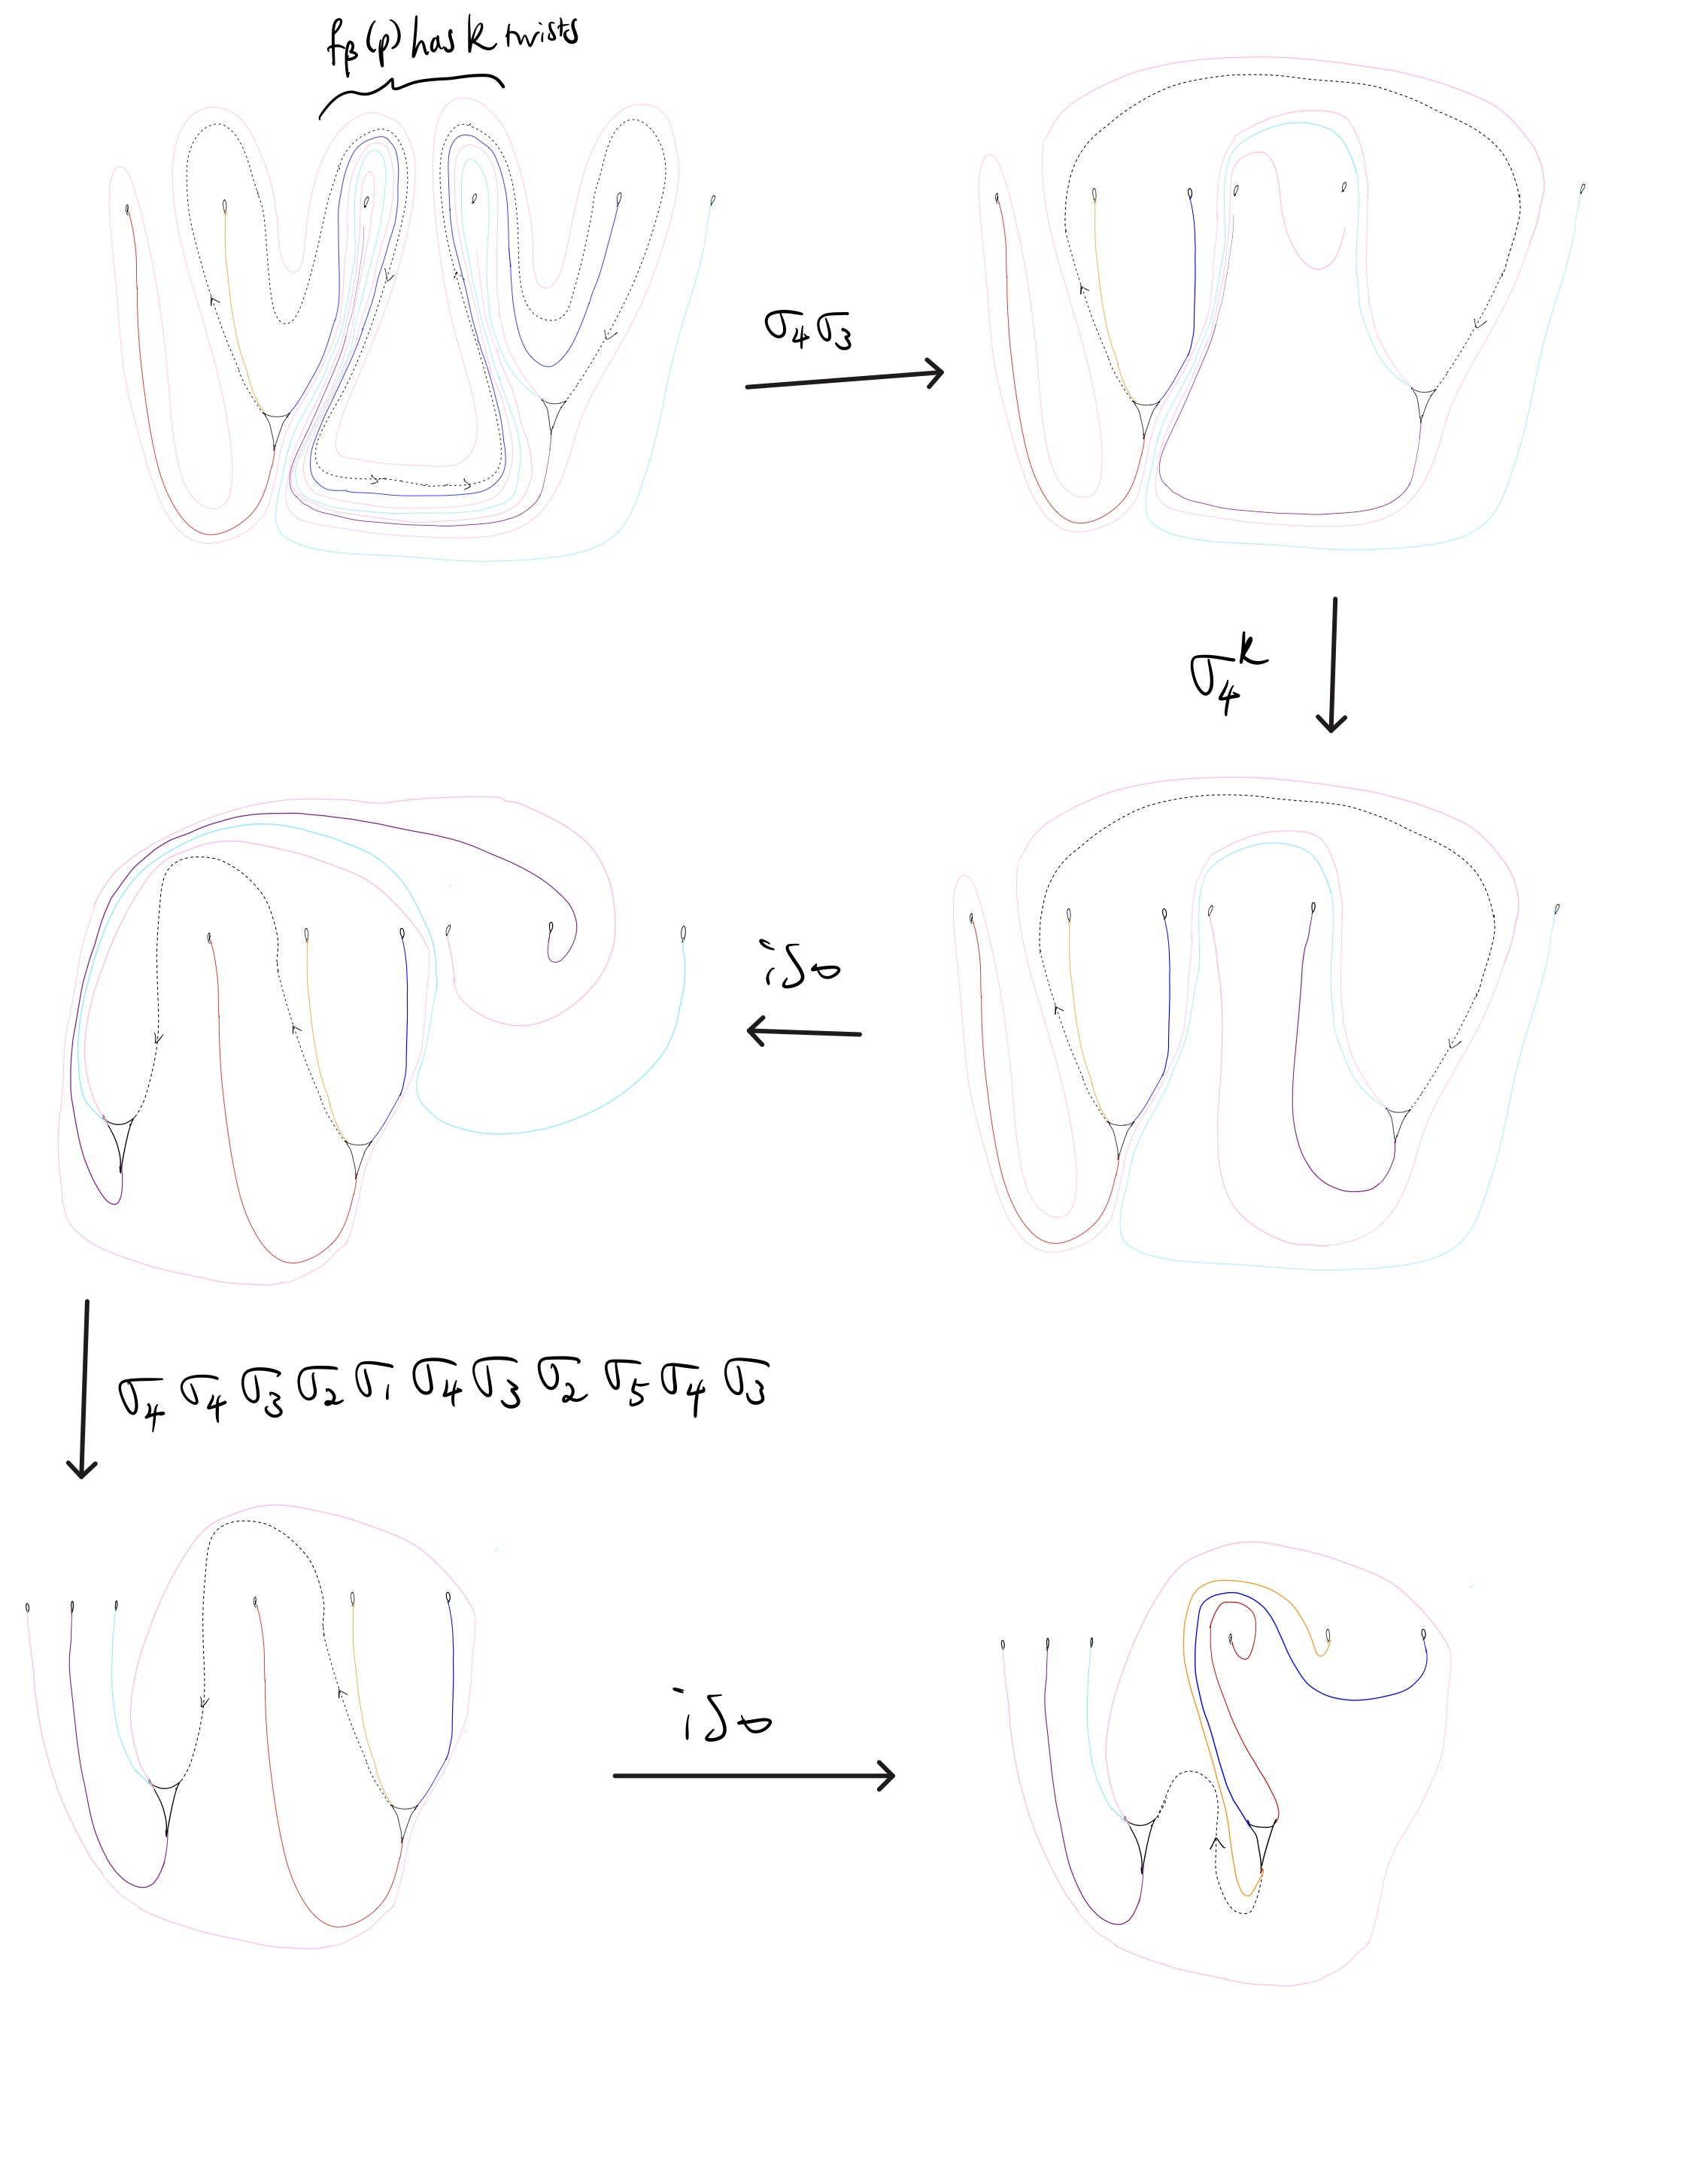
\includegraphics[width=\linewidth, height=0.45\textheight, keepaspectratio]{figures_braid/figures_track_1/Track 1 Braid 6 Abscond-2.jpg}\\
    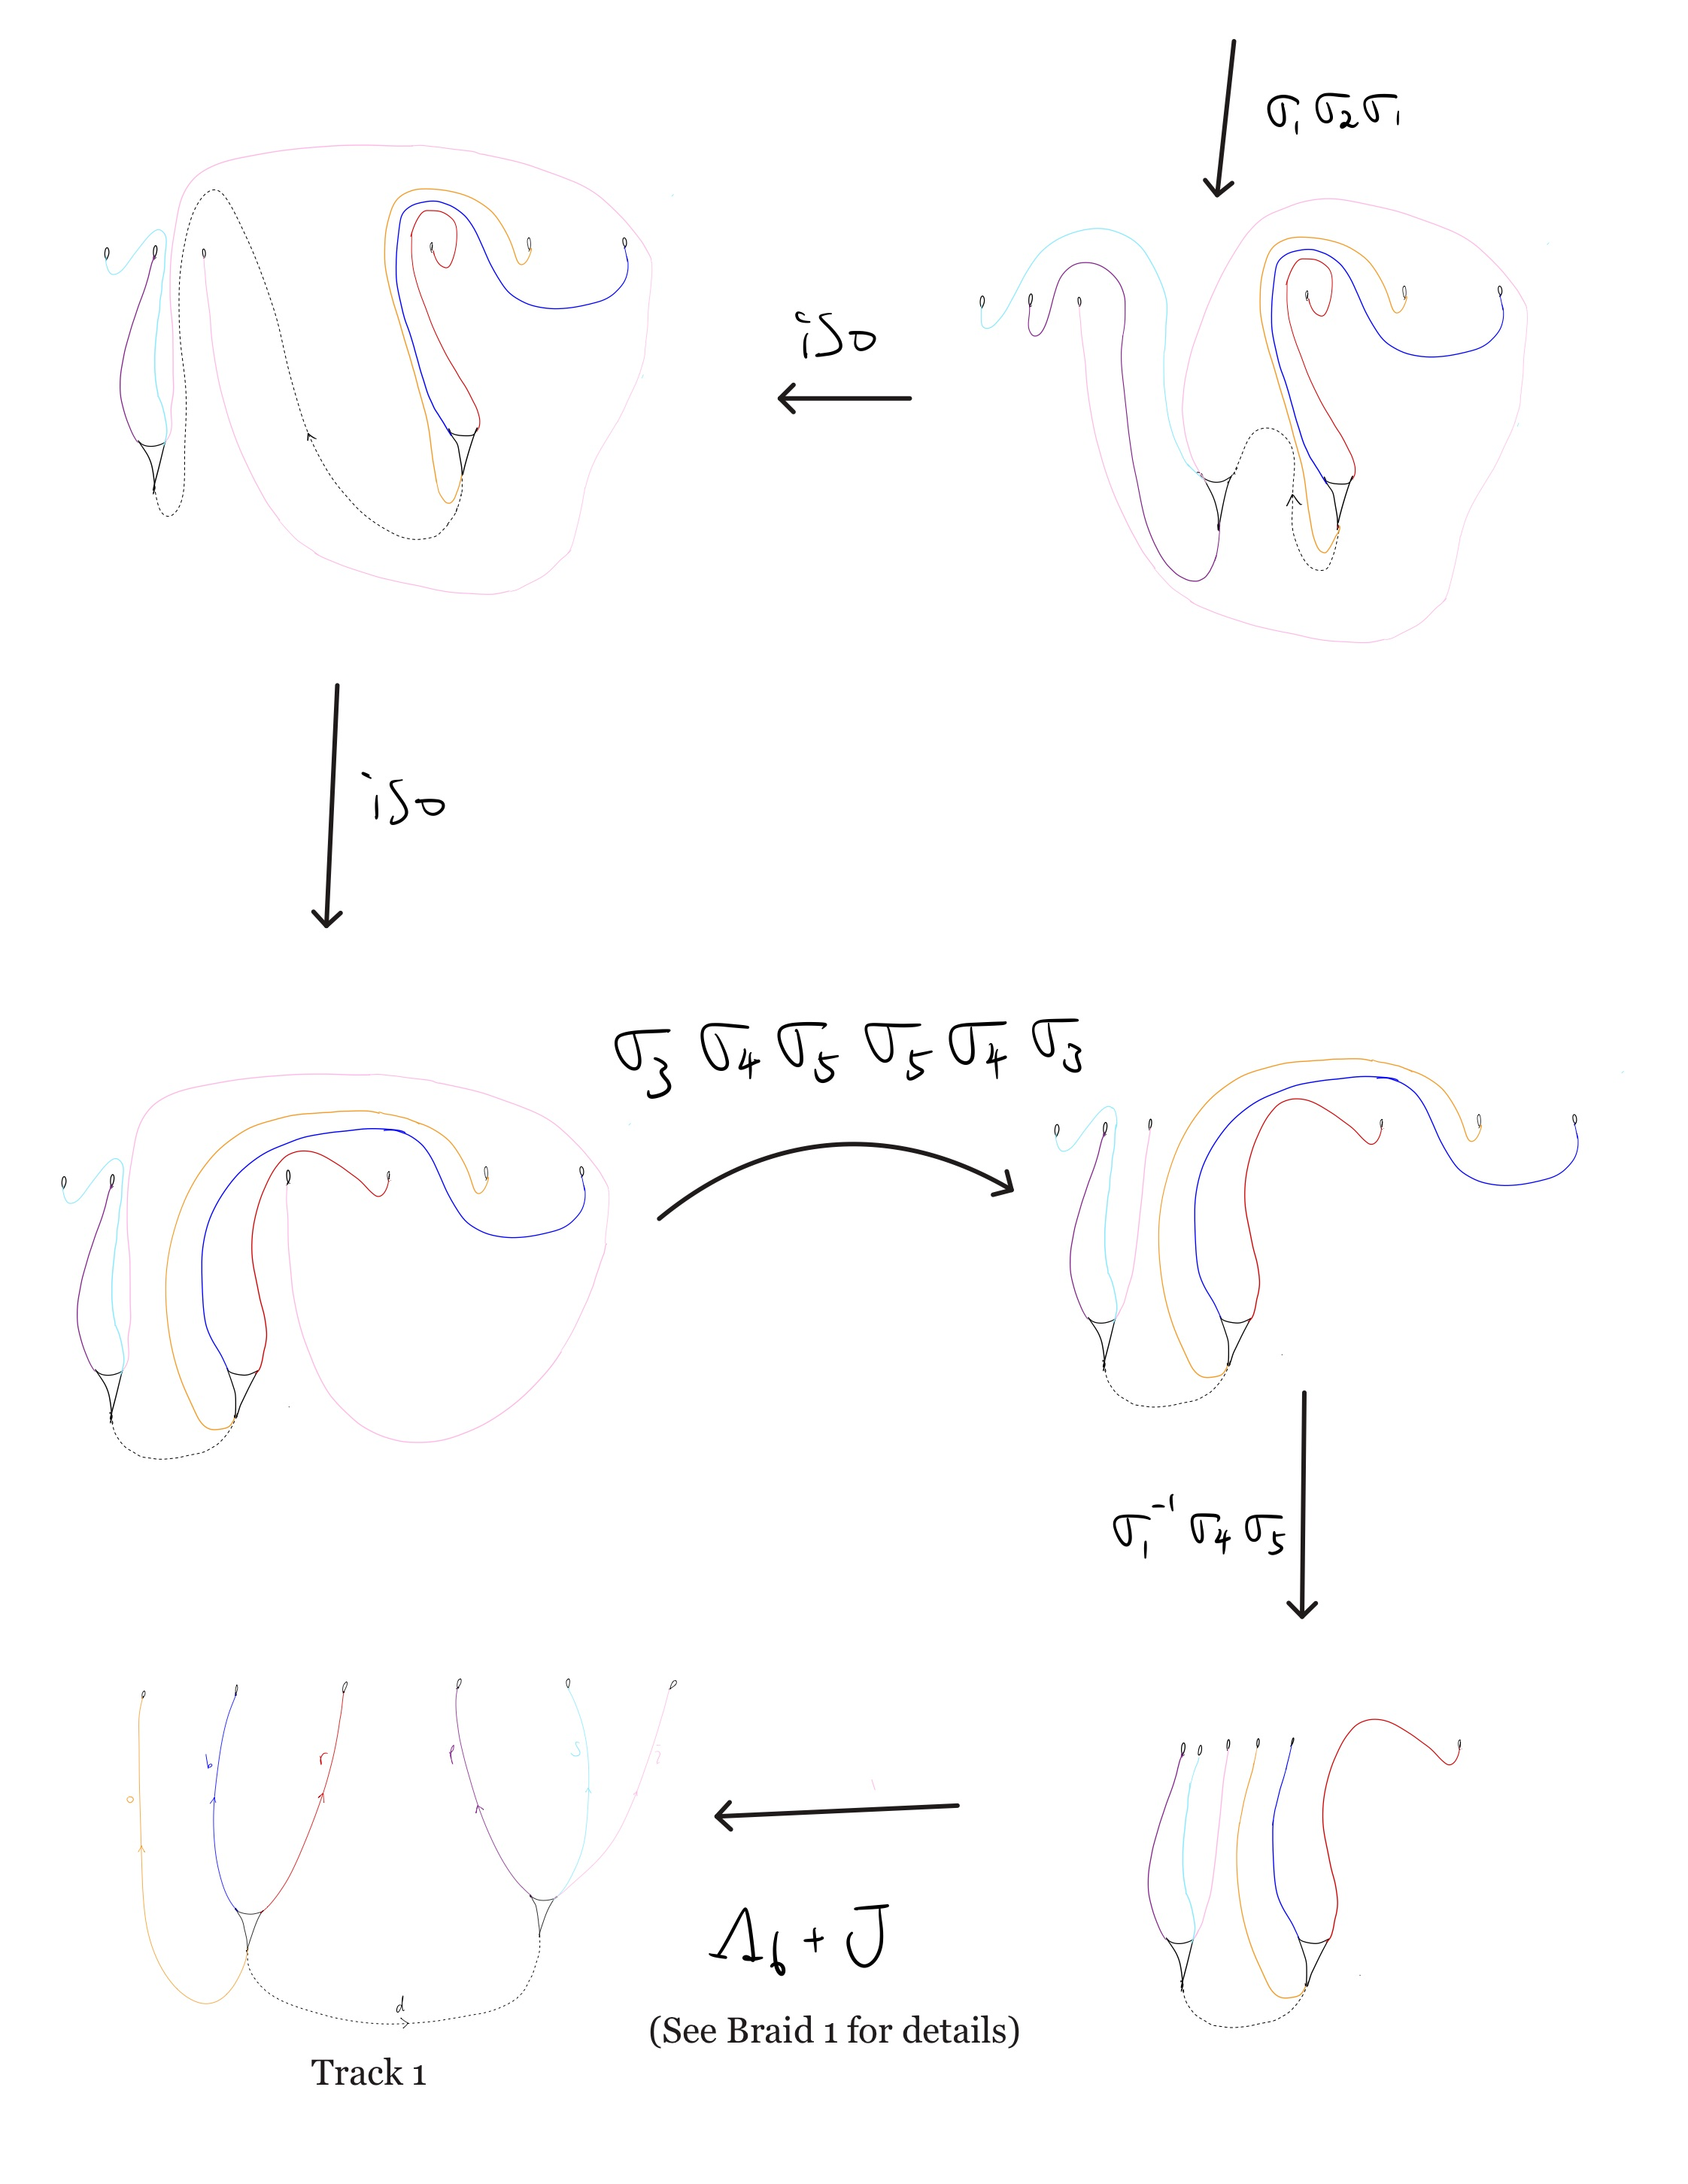
\includegraphics[width=\linewidth, height=0.45\textheight, keepaspectratio]{figures_braid/figures_track_1/Track 1 Braid 6 Abscond-3.jpg}
    \caption{This sequence shows the inverse of the braid $b_6^1$ carries Train Track Candidate Family 6.}
    \label{fig:track1_braid_b1_6}
\end{figure*}

\clearpage

\section{Candidate Family 7 (Fervent)}\label{sec:track1_fervent}
Train Track Map Candidate Family 7 of Track 1 is shown in Figure \ref{fig:track1_braid_b1_7_map}. See \ref{Fervent} for details.

\begin{figure*}[ht]
    \centering
    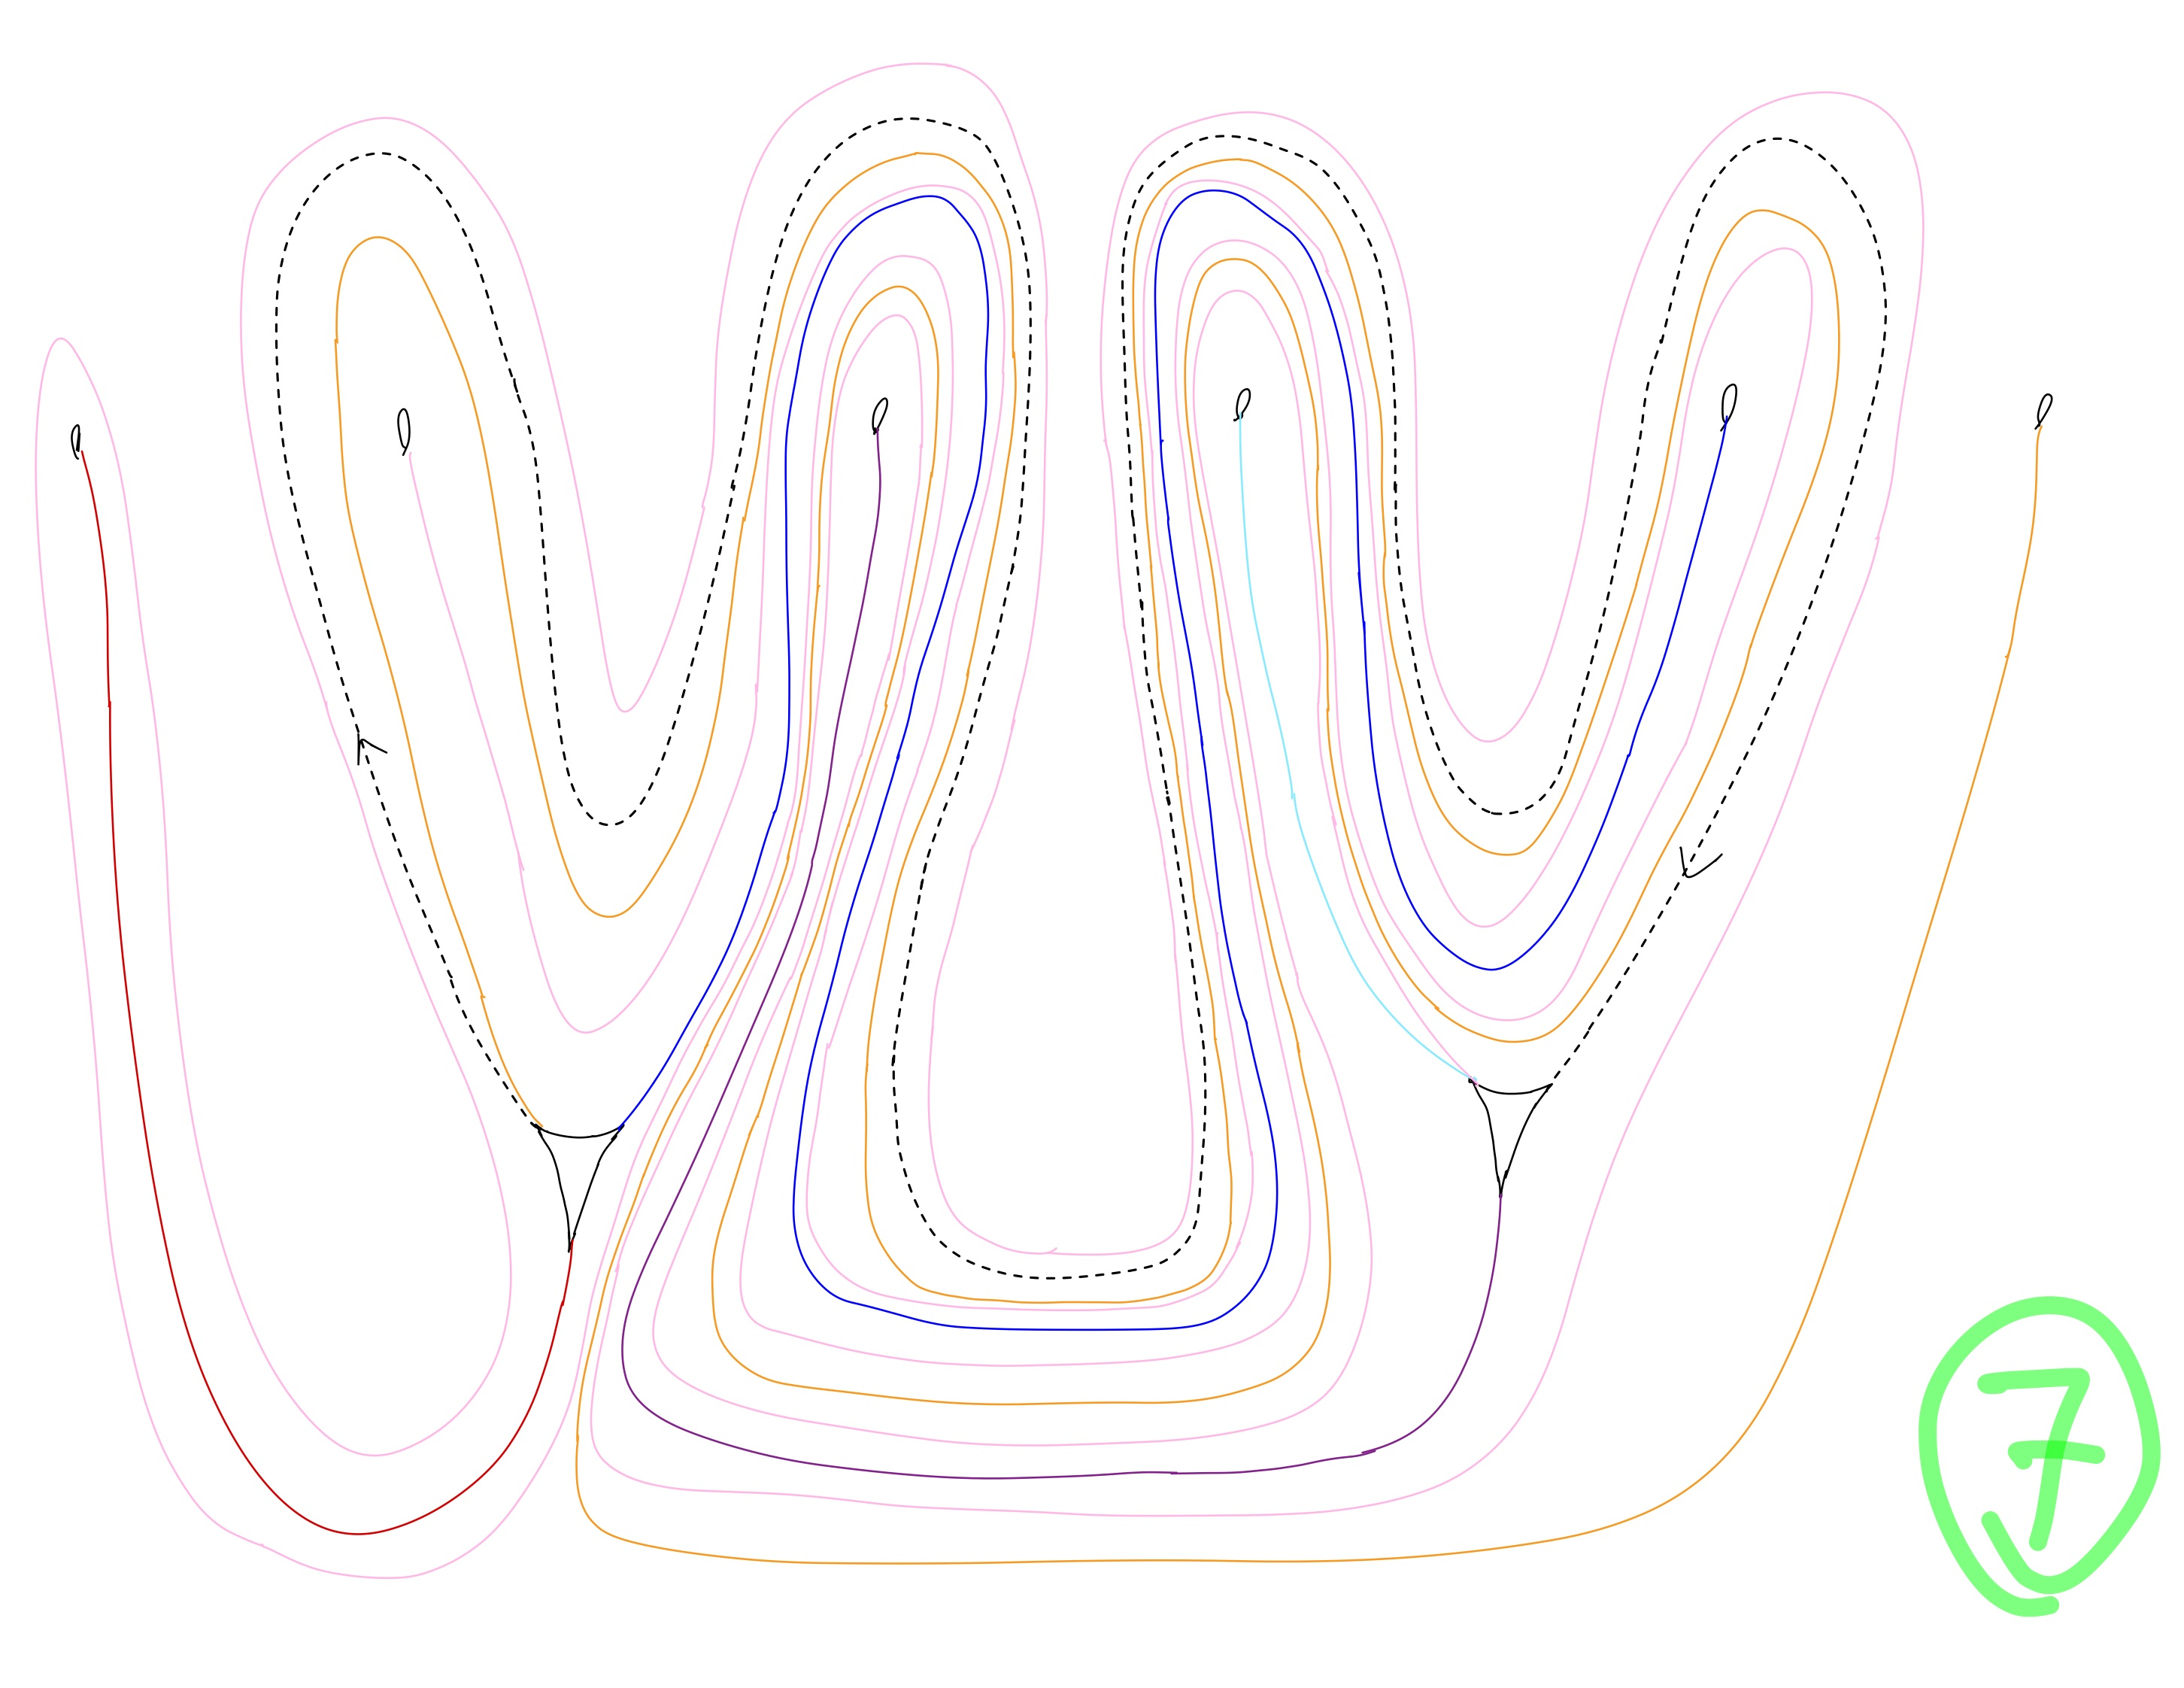
\includegraphics[width=\linewidth, height=0.45\textheight, keepaspectratio]{figures_braid/figures_track_1/Track 1 Braid 7 Fervent-1.jpg}
    \caption{Train Track Map Candidate Family 7 (Fervent) of Track 1.}
    \label{fig:track1_braid_b1_7_map}
\end{figure*}

The inverse of the following braid carries this family of train track maps:
\[
b_7^1 = \sigma_{2}^{-1} \sigma_{3}^{-1} \sigma_{4}^{-1} \sigma_{3} \sigma_{2} \sigma_{4} \sigma_{3} \sigma_{4} \sigma_{4} \sigma_{3} \sigma_{2} \sigma_{1} \sigma_{4} \sigma_{3} \sigma_{2} \sigma_{4}^{-1} \sigma_{3}^{-1} \sigma_{2}^{-1} \sigma_{1}^{-1} \sigma_{1}^{-1} \sigma_{2}^{-1} \sigma_{5} \sigma_{4} \sigma_{5} \circ J \circ \Lambda_6
\]

This is shown in Figure \ref{fig:track1_braid_b1_7}.

\begin{figure*}[p]
    \centering
    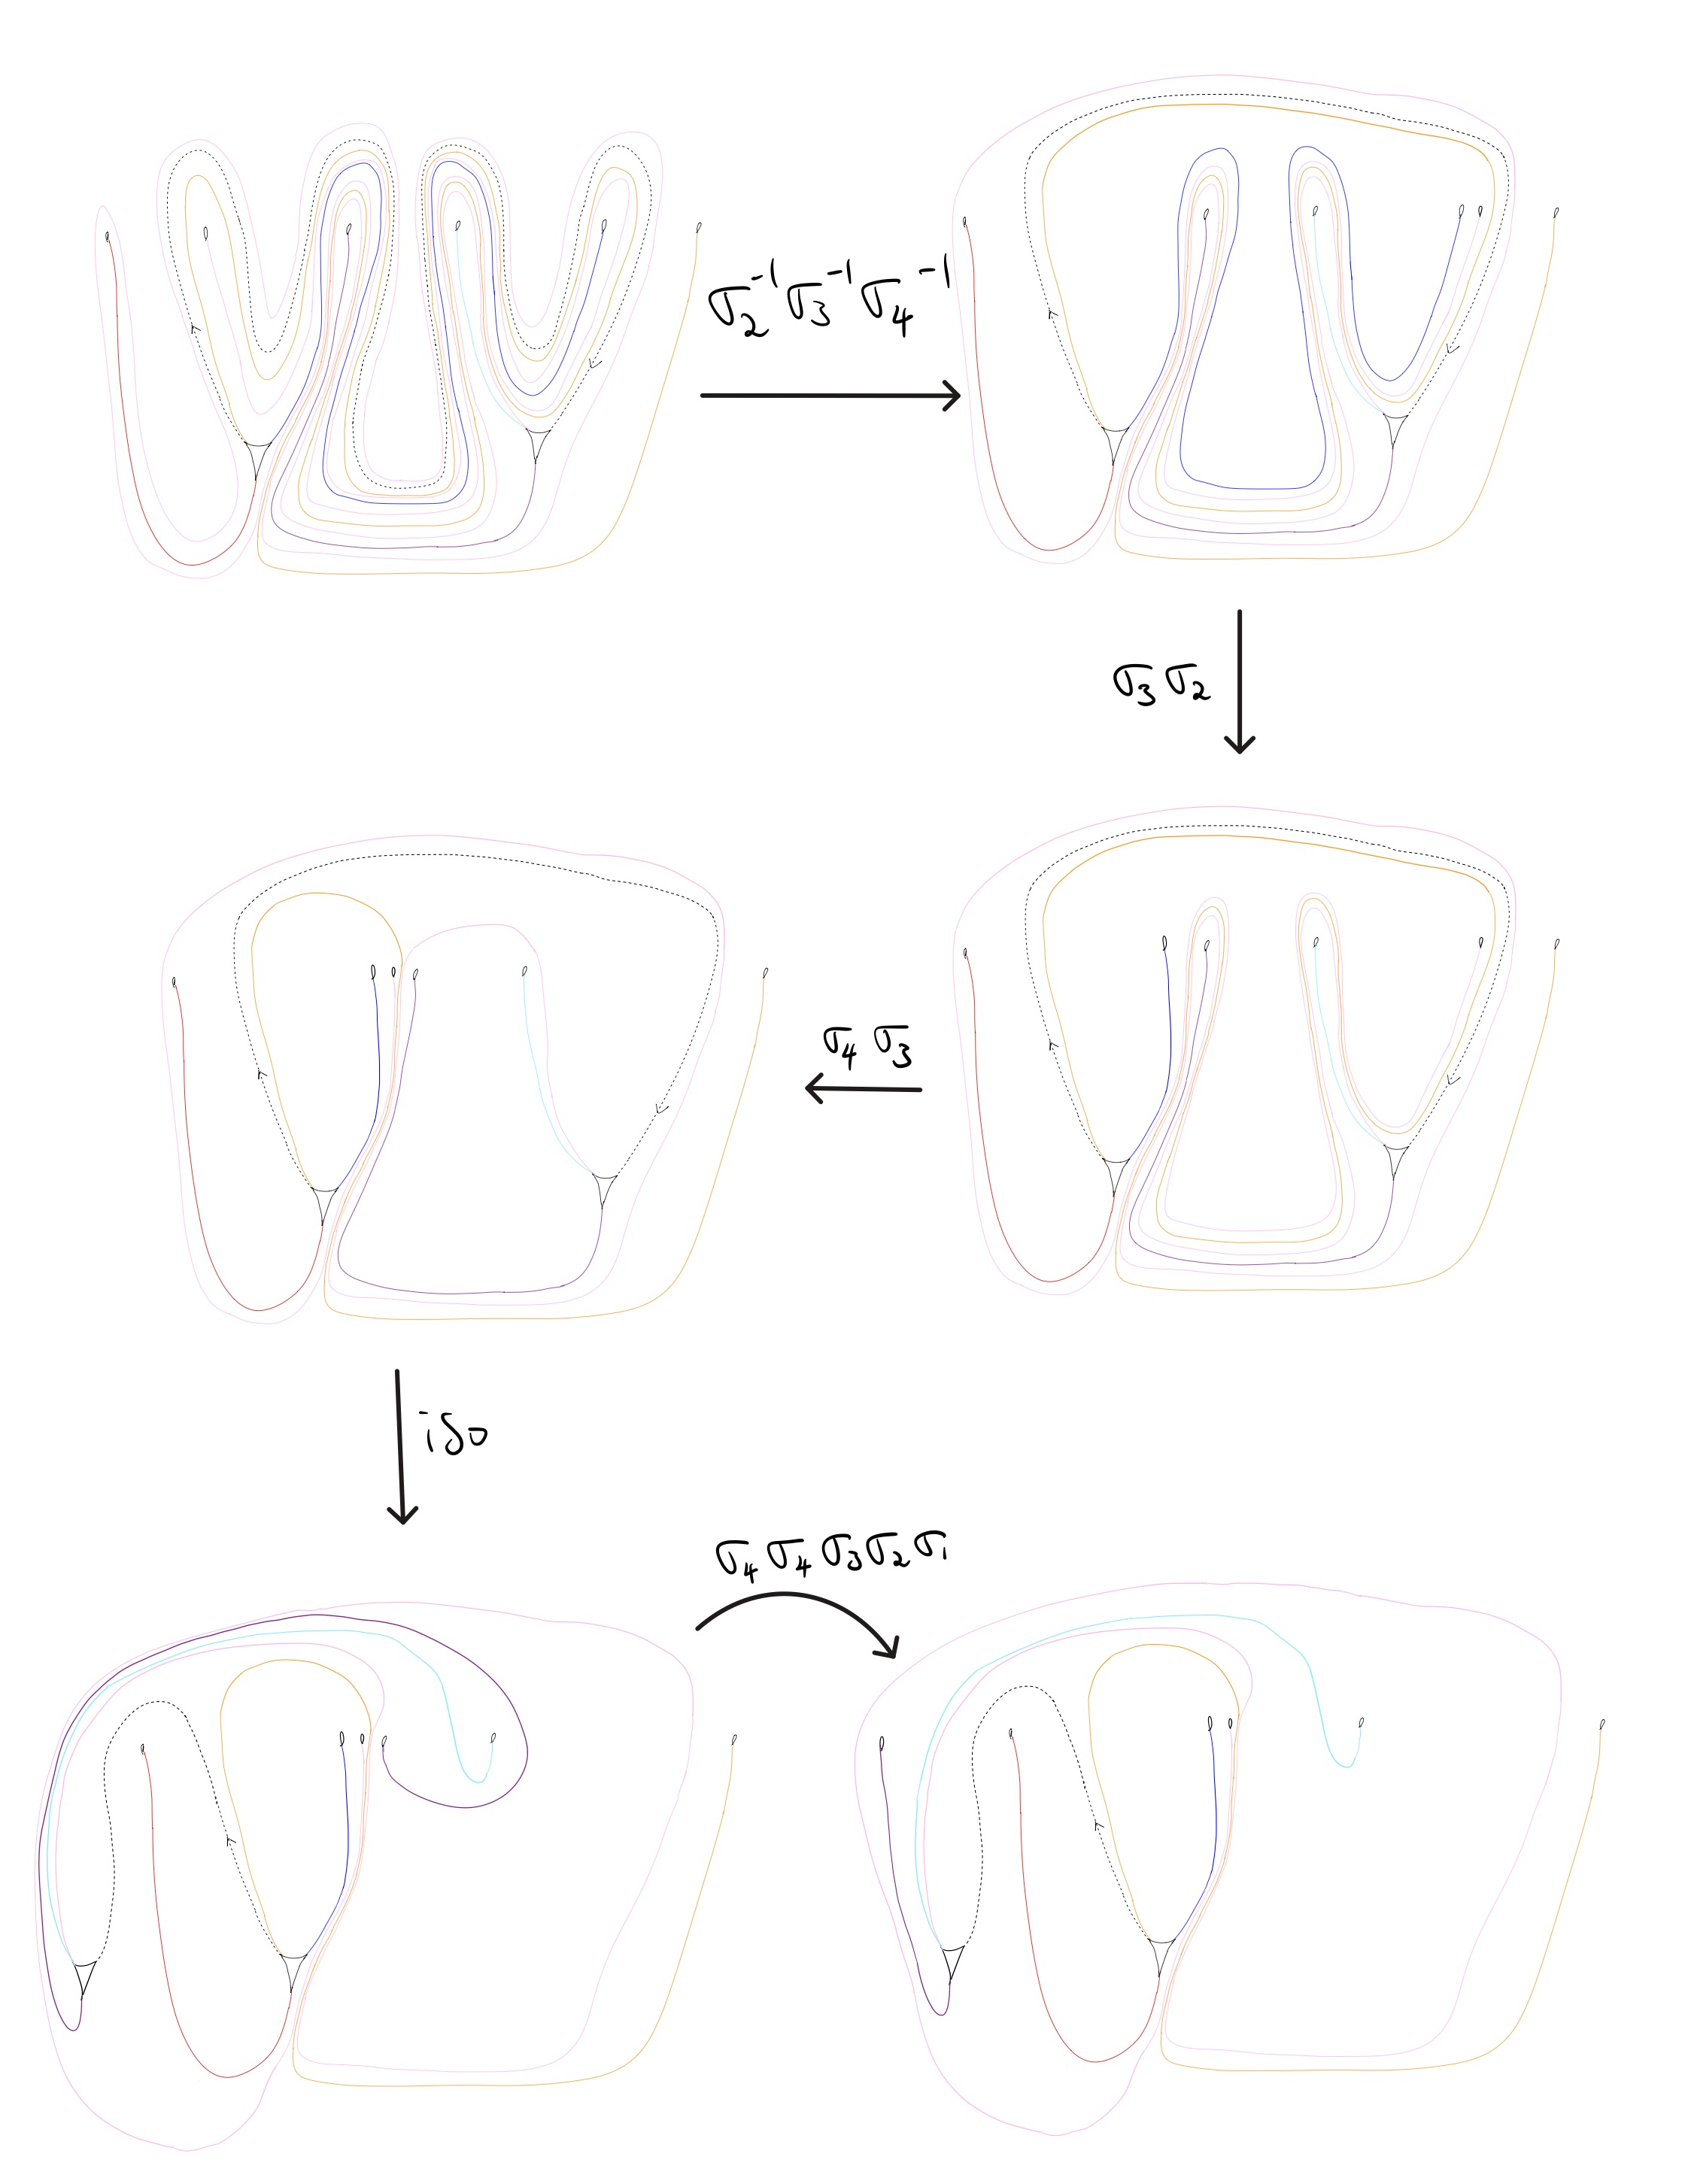
\includegraphics[width=\linewidth, height=0.45\textheight, keepaspectratio]{figures_braid/figures_track_1/Track 1 Braid 7 Fervent-2.jpg}\\
    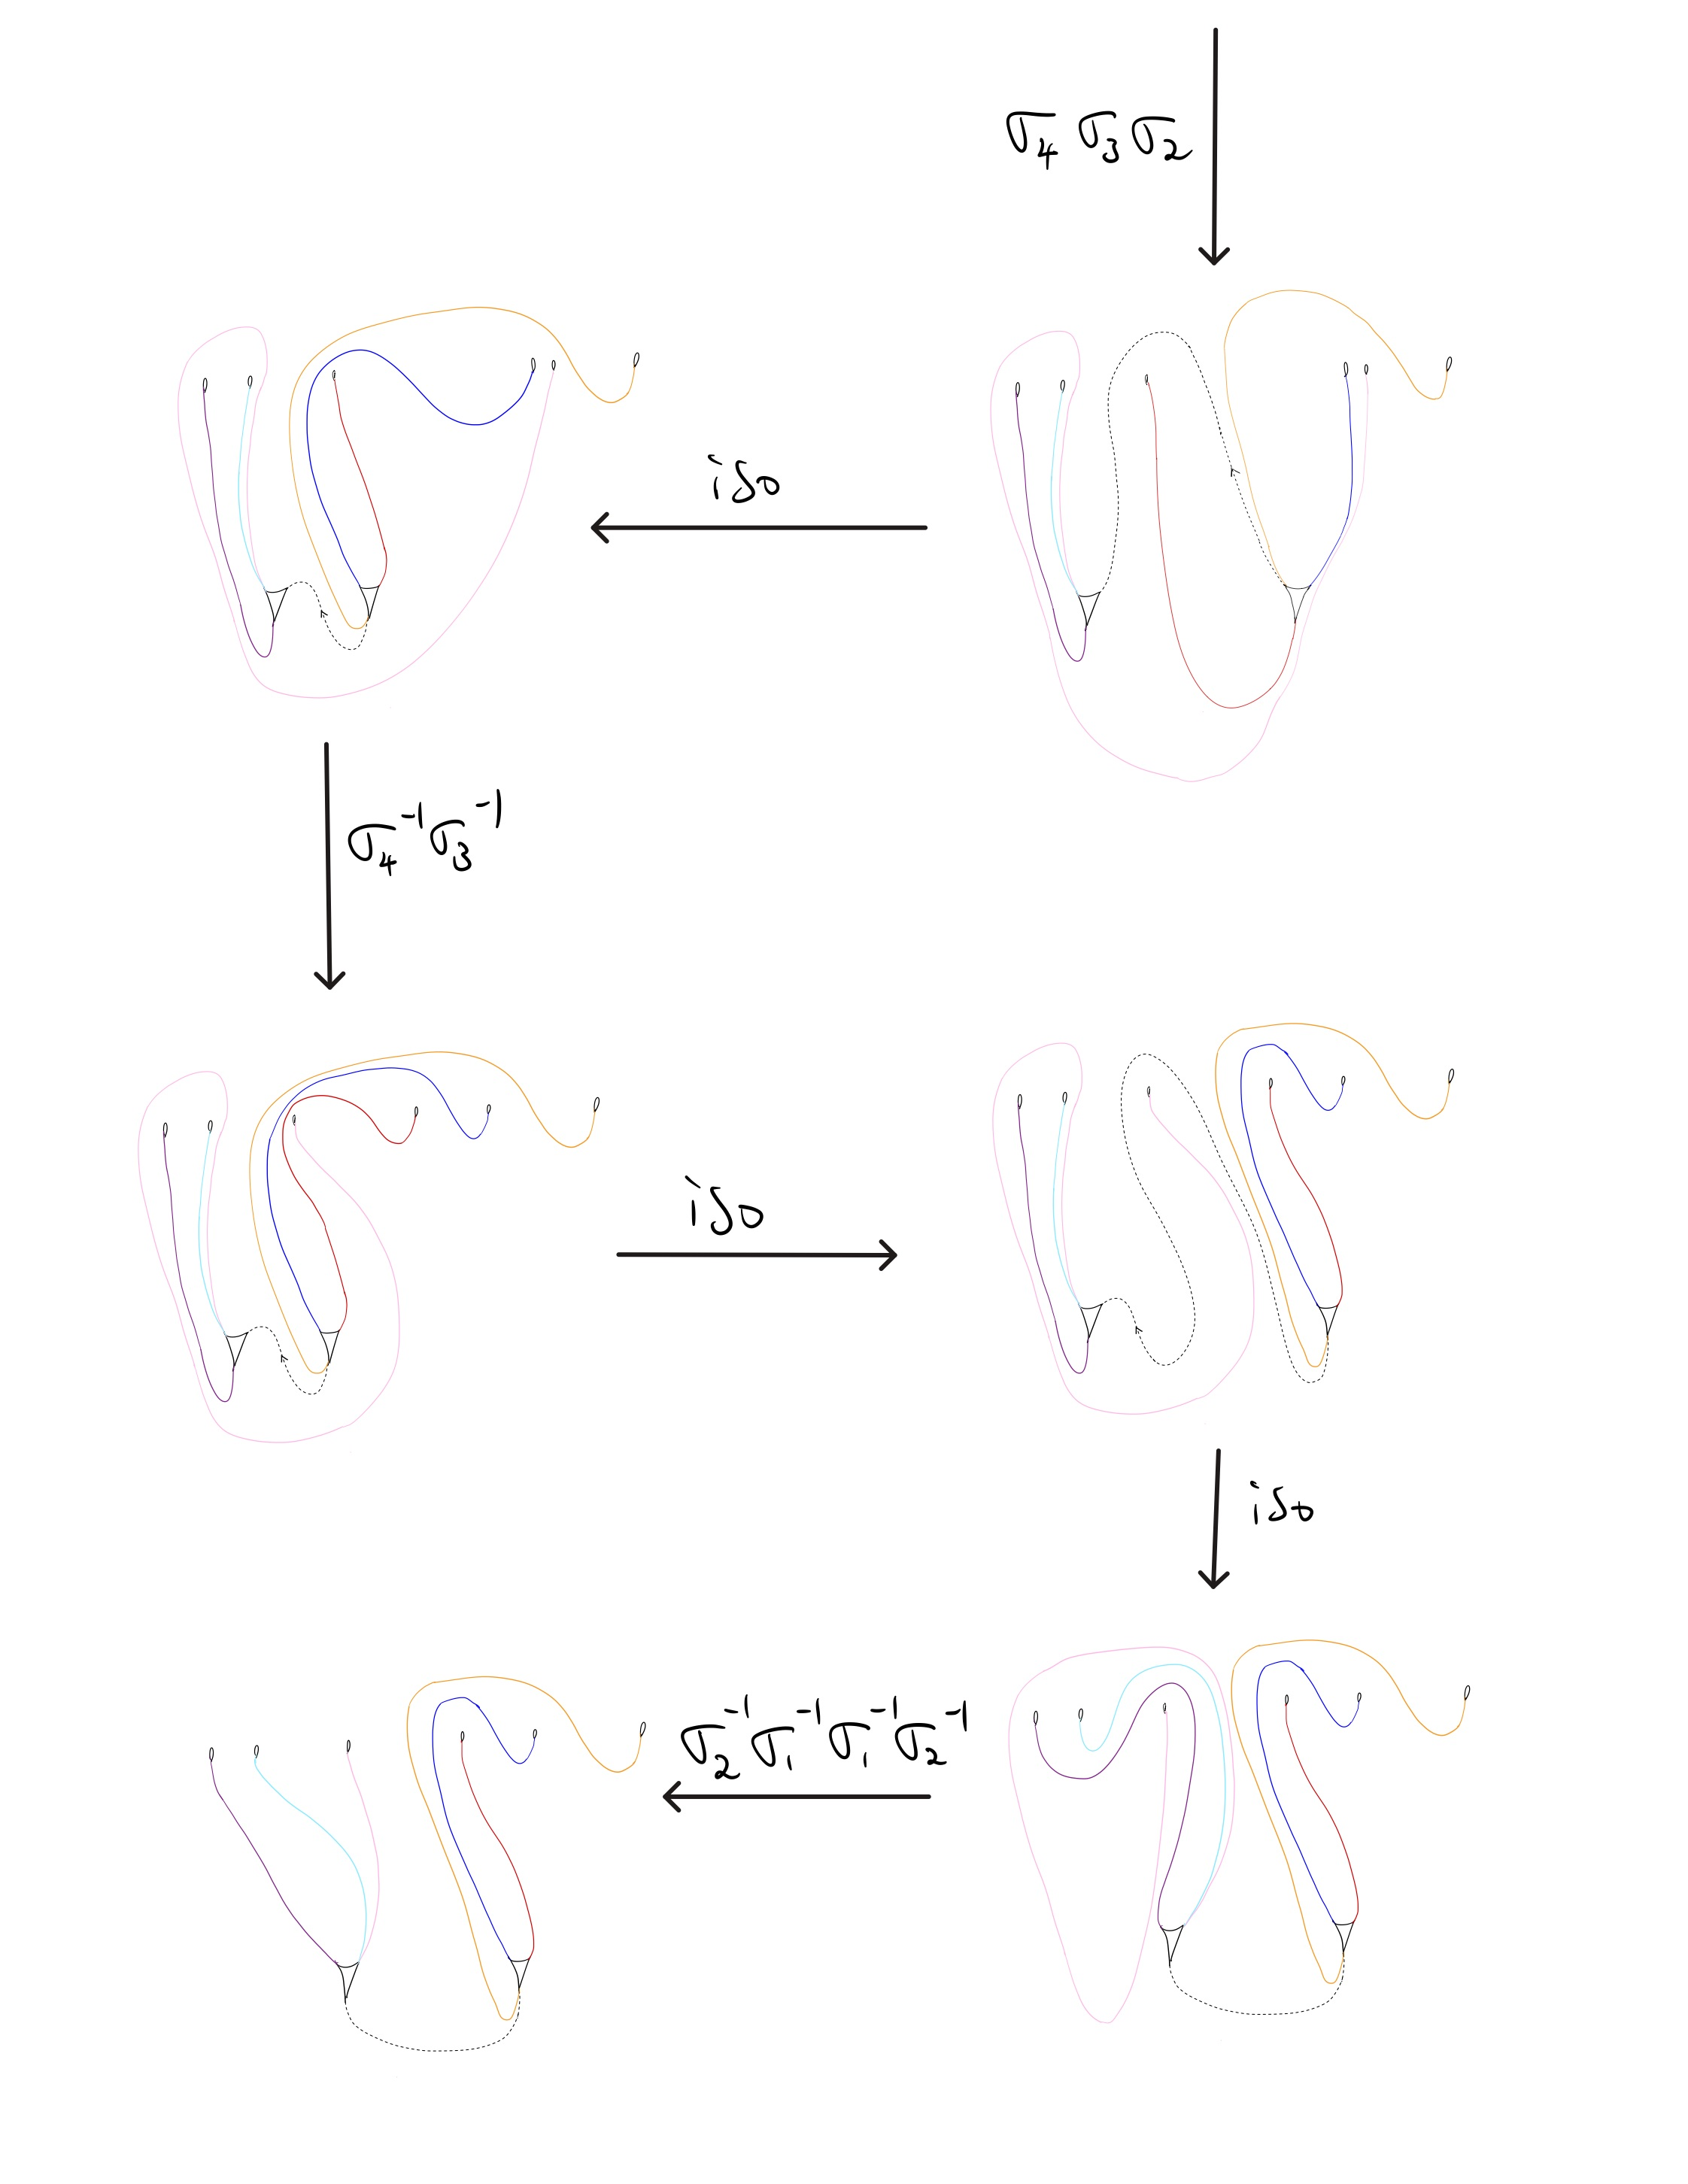
\includegraphics[width=\linewidth, height=0.45\textheight, keepaspectratio]{figures_braid/figures_track_1/Track 1 Braid 7 Fervent-3.jpg}
    \caption{This sequence shows the inverse of the braid $b_7^1$ carries Train Track Candidate Family 7.}
    \label{fig:track1_braid_b1_7}
\end{figure*}

\clearpage

\section{Candidate Family 8 (Panorama)}\label{sec:track1_panorama}
Train Track Map Candidate Family 8 of Track 1 is shown in Figure \ref{fig:track1_braid_b1_8_map}. See \ref{Panorama} for details.

\begin{figure*}[ht]
    \centering
    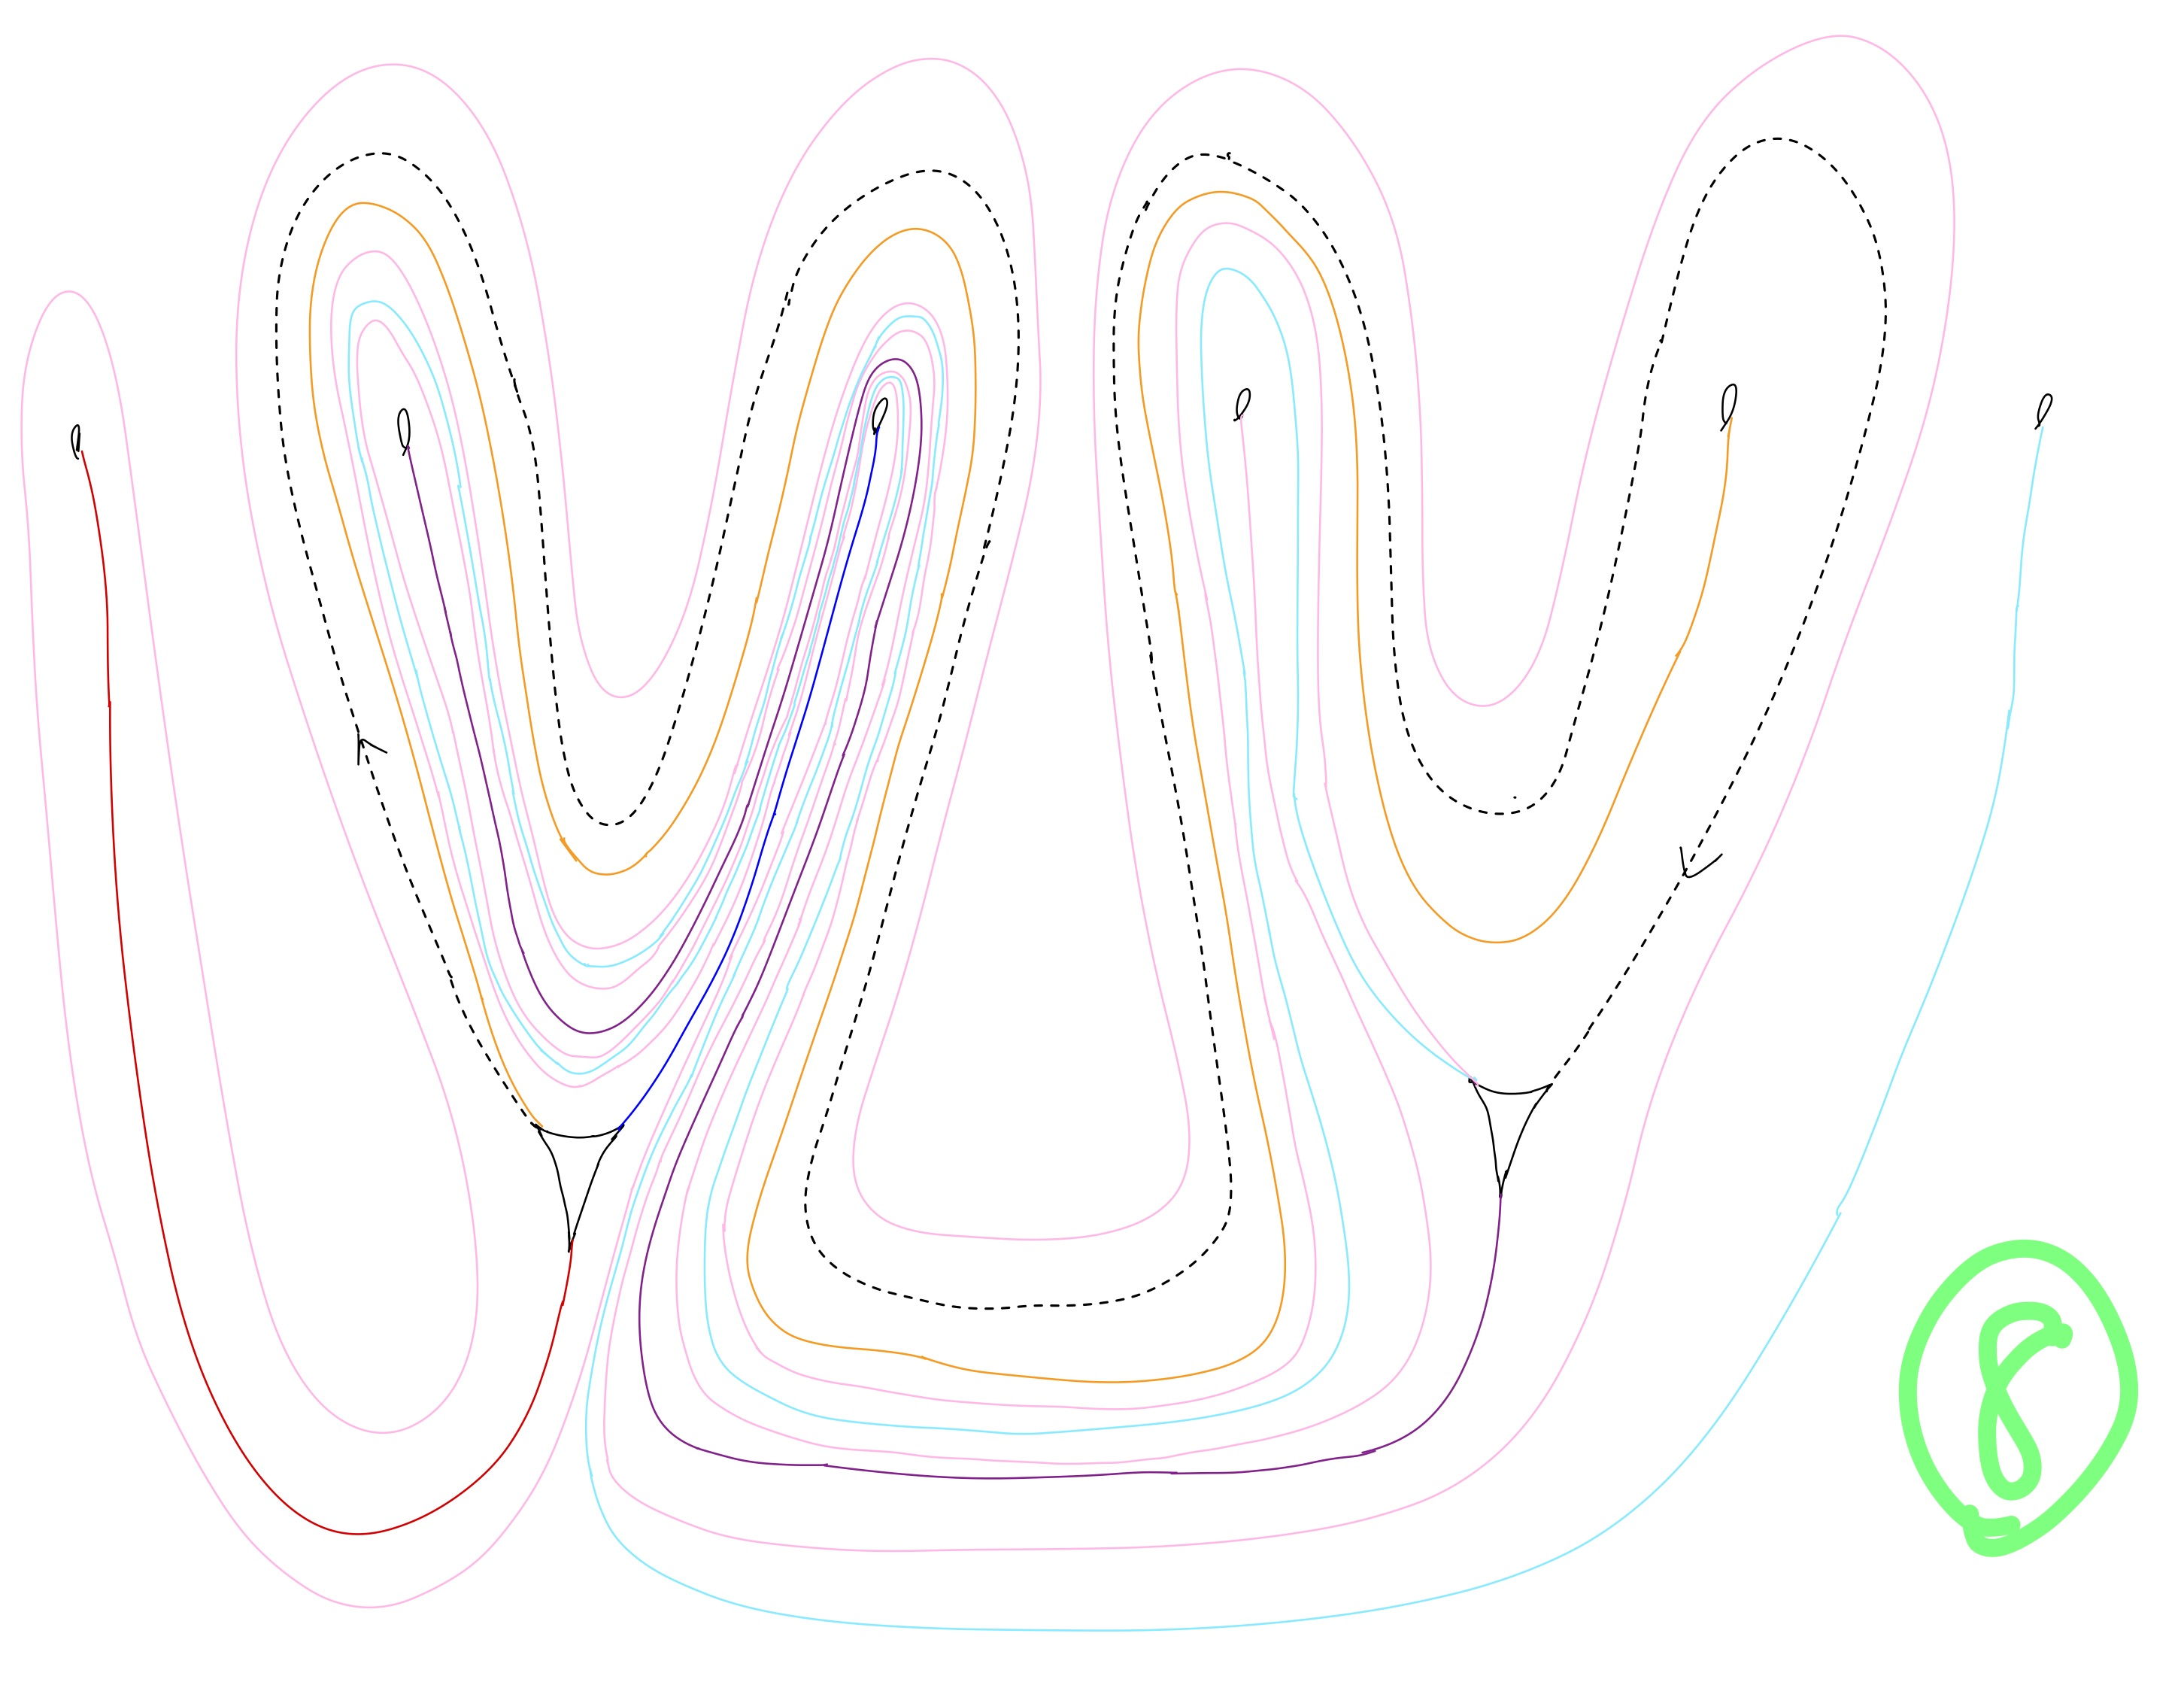
\includegraphics[width=\linewidth, height=0.45\textheight, keepaspectratio]{figures_braid/figures_track_1/Track 1 Braid 8 Panorama-1.jpg}
    \caption{Train Track Map Candidate Family 8 (Panorama) of Track 1.}
    \label{fig:track1_braid_b1_8_map}
\end{figure*}

The inverse of the following braid carries this family of train track maps:
\[
b_8^1 = \sigma_{4} \sigma_{3} \sigma_{2} \sigma_{4} \sigma_{3} \sigma_{4}^{-1} \sigma_{3}^{-1} \sigma_{4} \sigma_{4} \sigma_{3} \sigma_{2} \sigma_{1} \sigma_{4} \sigma_{3} \sigma_{2} \sigma_{5} \sigma_{4} \sigma_{3} \sigma_{3}^{-1} \sigma_{4}^{-1} \sigma_{5}^{-1} \sigma_{2}^{-1} \sigma_{3}^{-1} \sigma_{4}^{-1} \sigma_{2}^{-1} \sigma_{3}^{-1} \sigma_{2}^{-1} \sigma_{2}^{-1} \sigma_{1} \sigma_{2} \sigma_{3} \sigma_{4} \sigma_{5}
\]

This is shown in Figure \ref{fig:track1_braid_b1_8}.

\begin{figure*}[p]
    \centering
    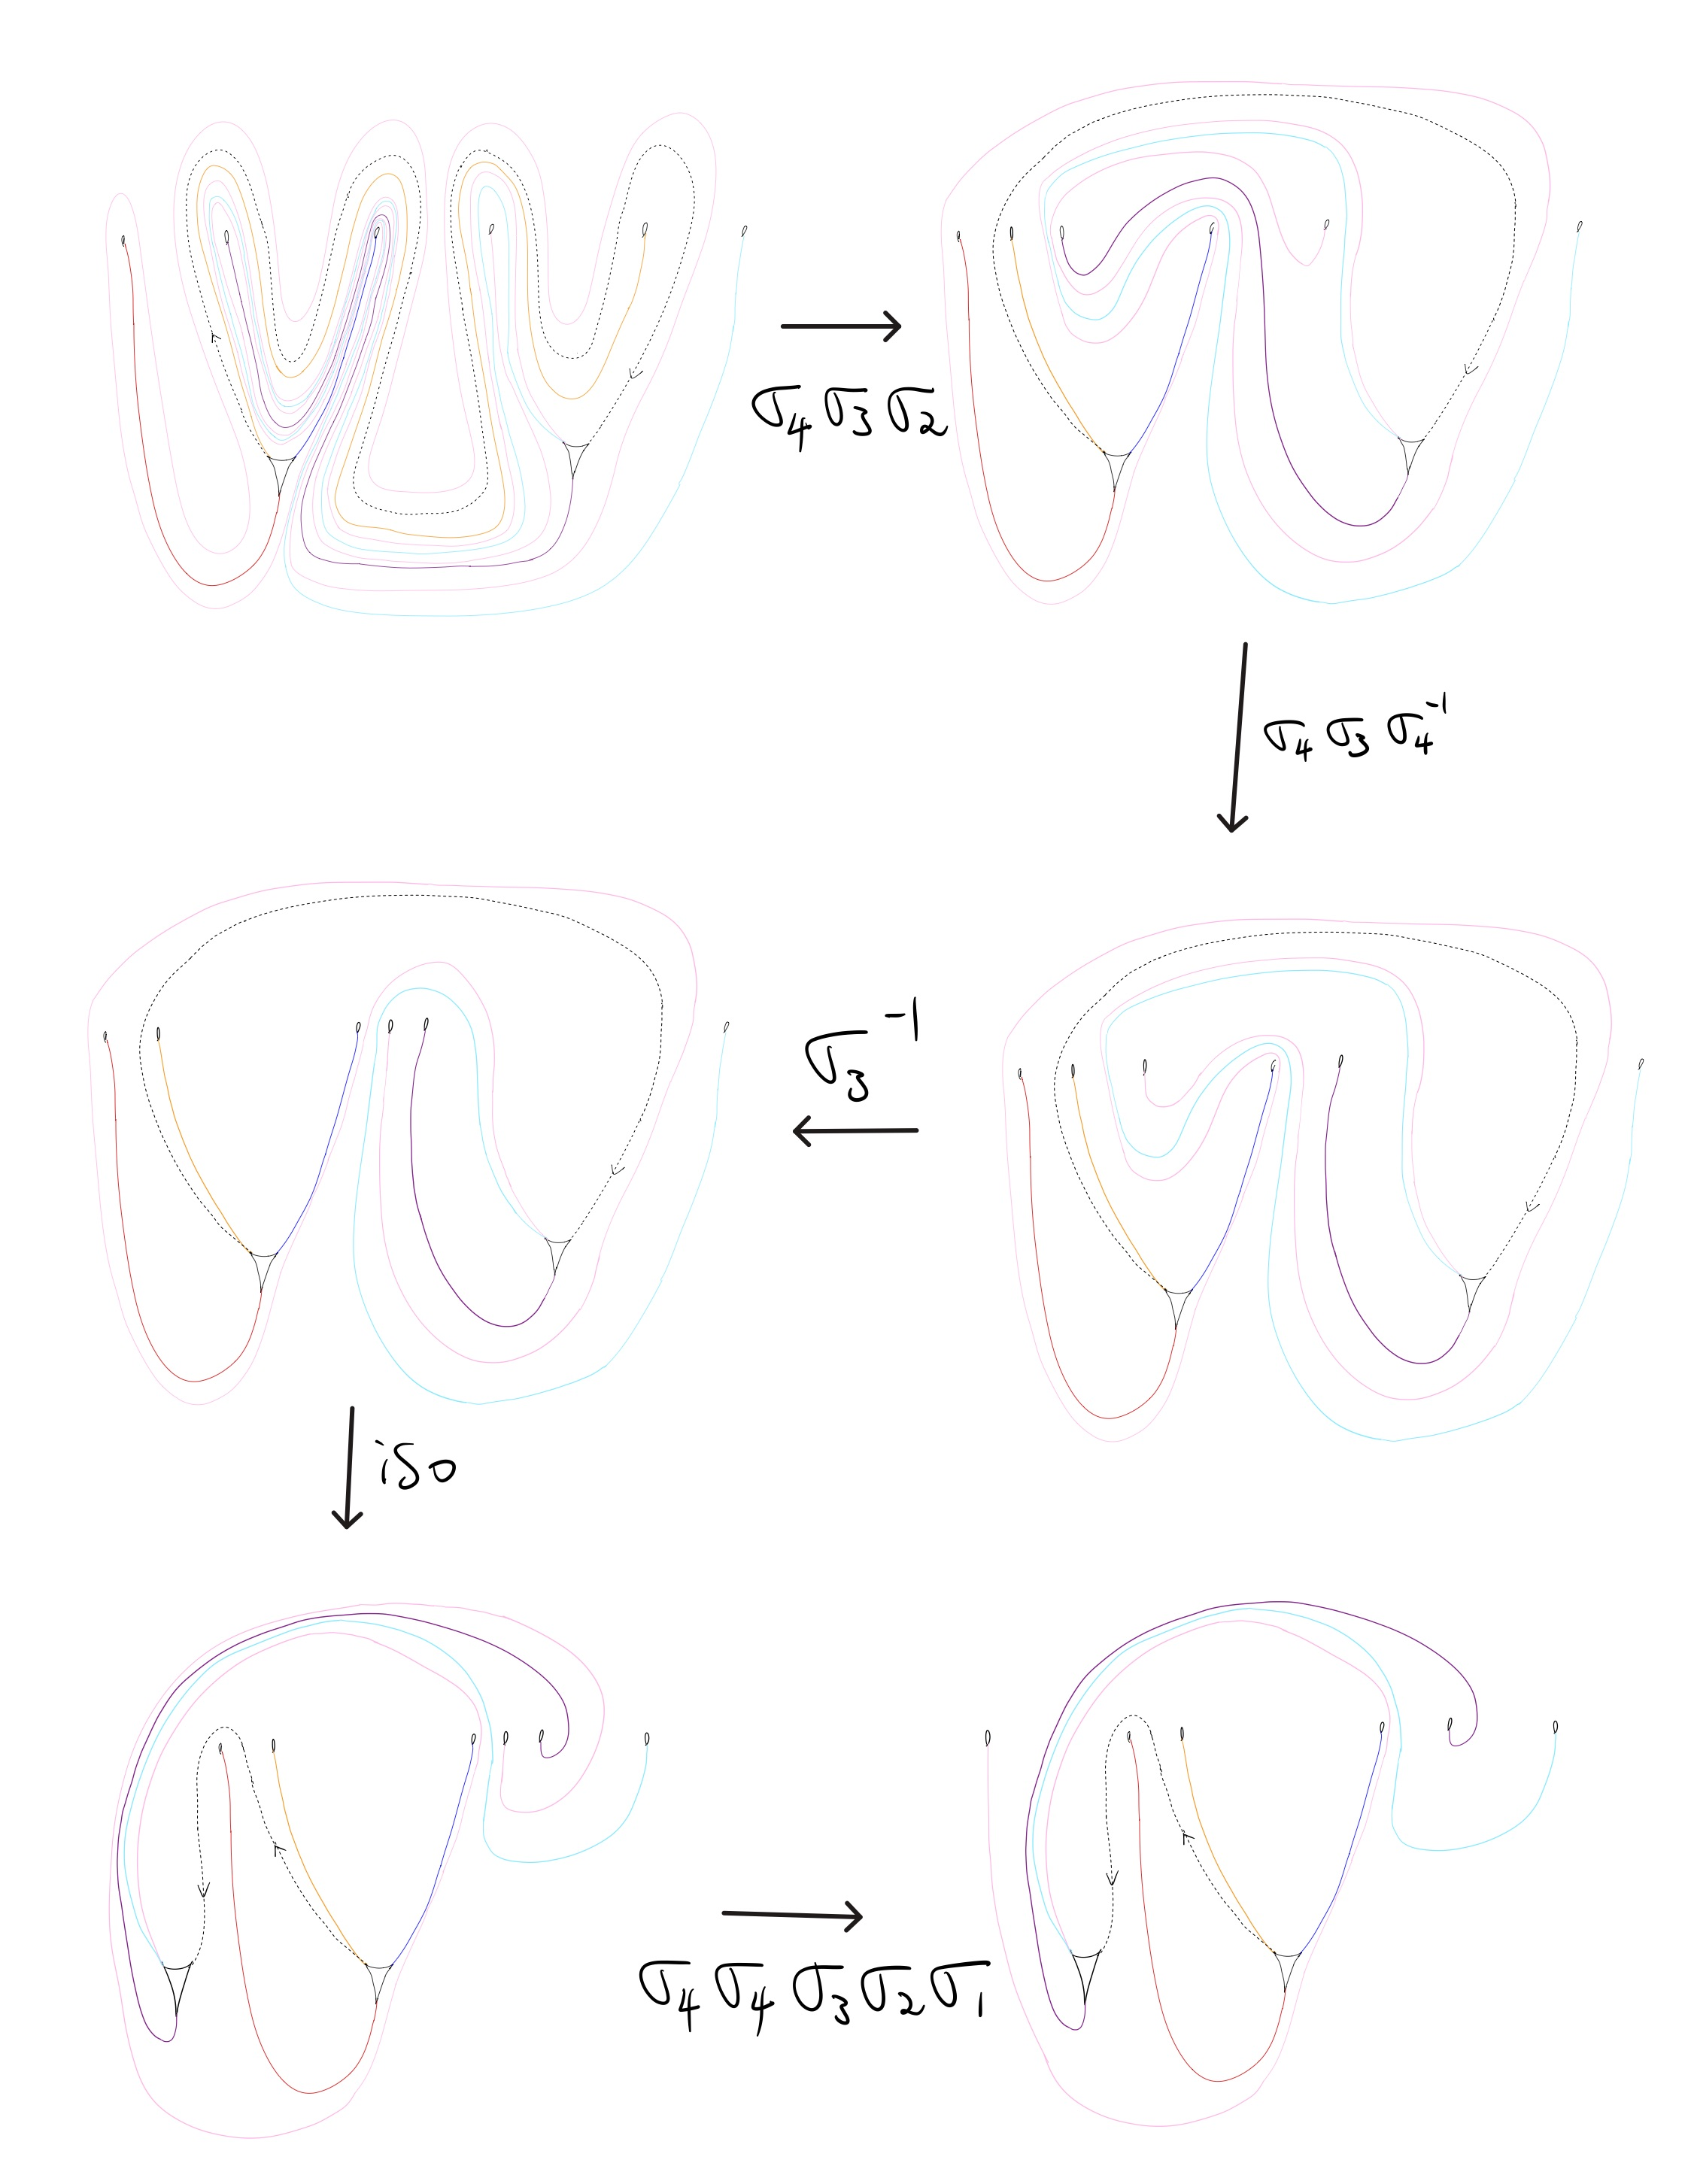
\includegraphics[width=\linewidth, height=0.45\textheight, keepaspectratio]{figures_braid/figures_track_1/Track 1 Braid 8 Panorama-2.jpg}\\
    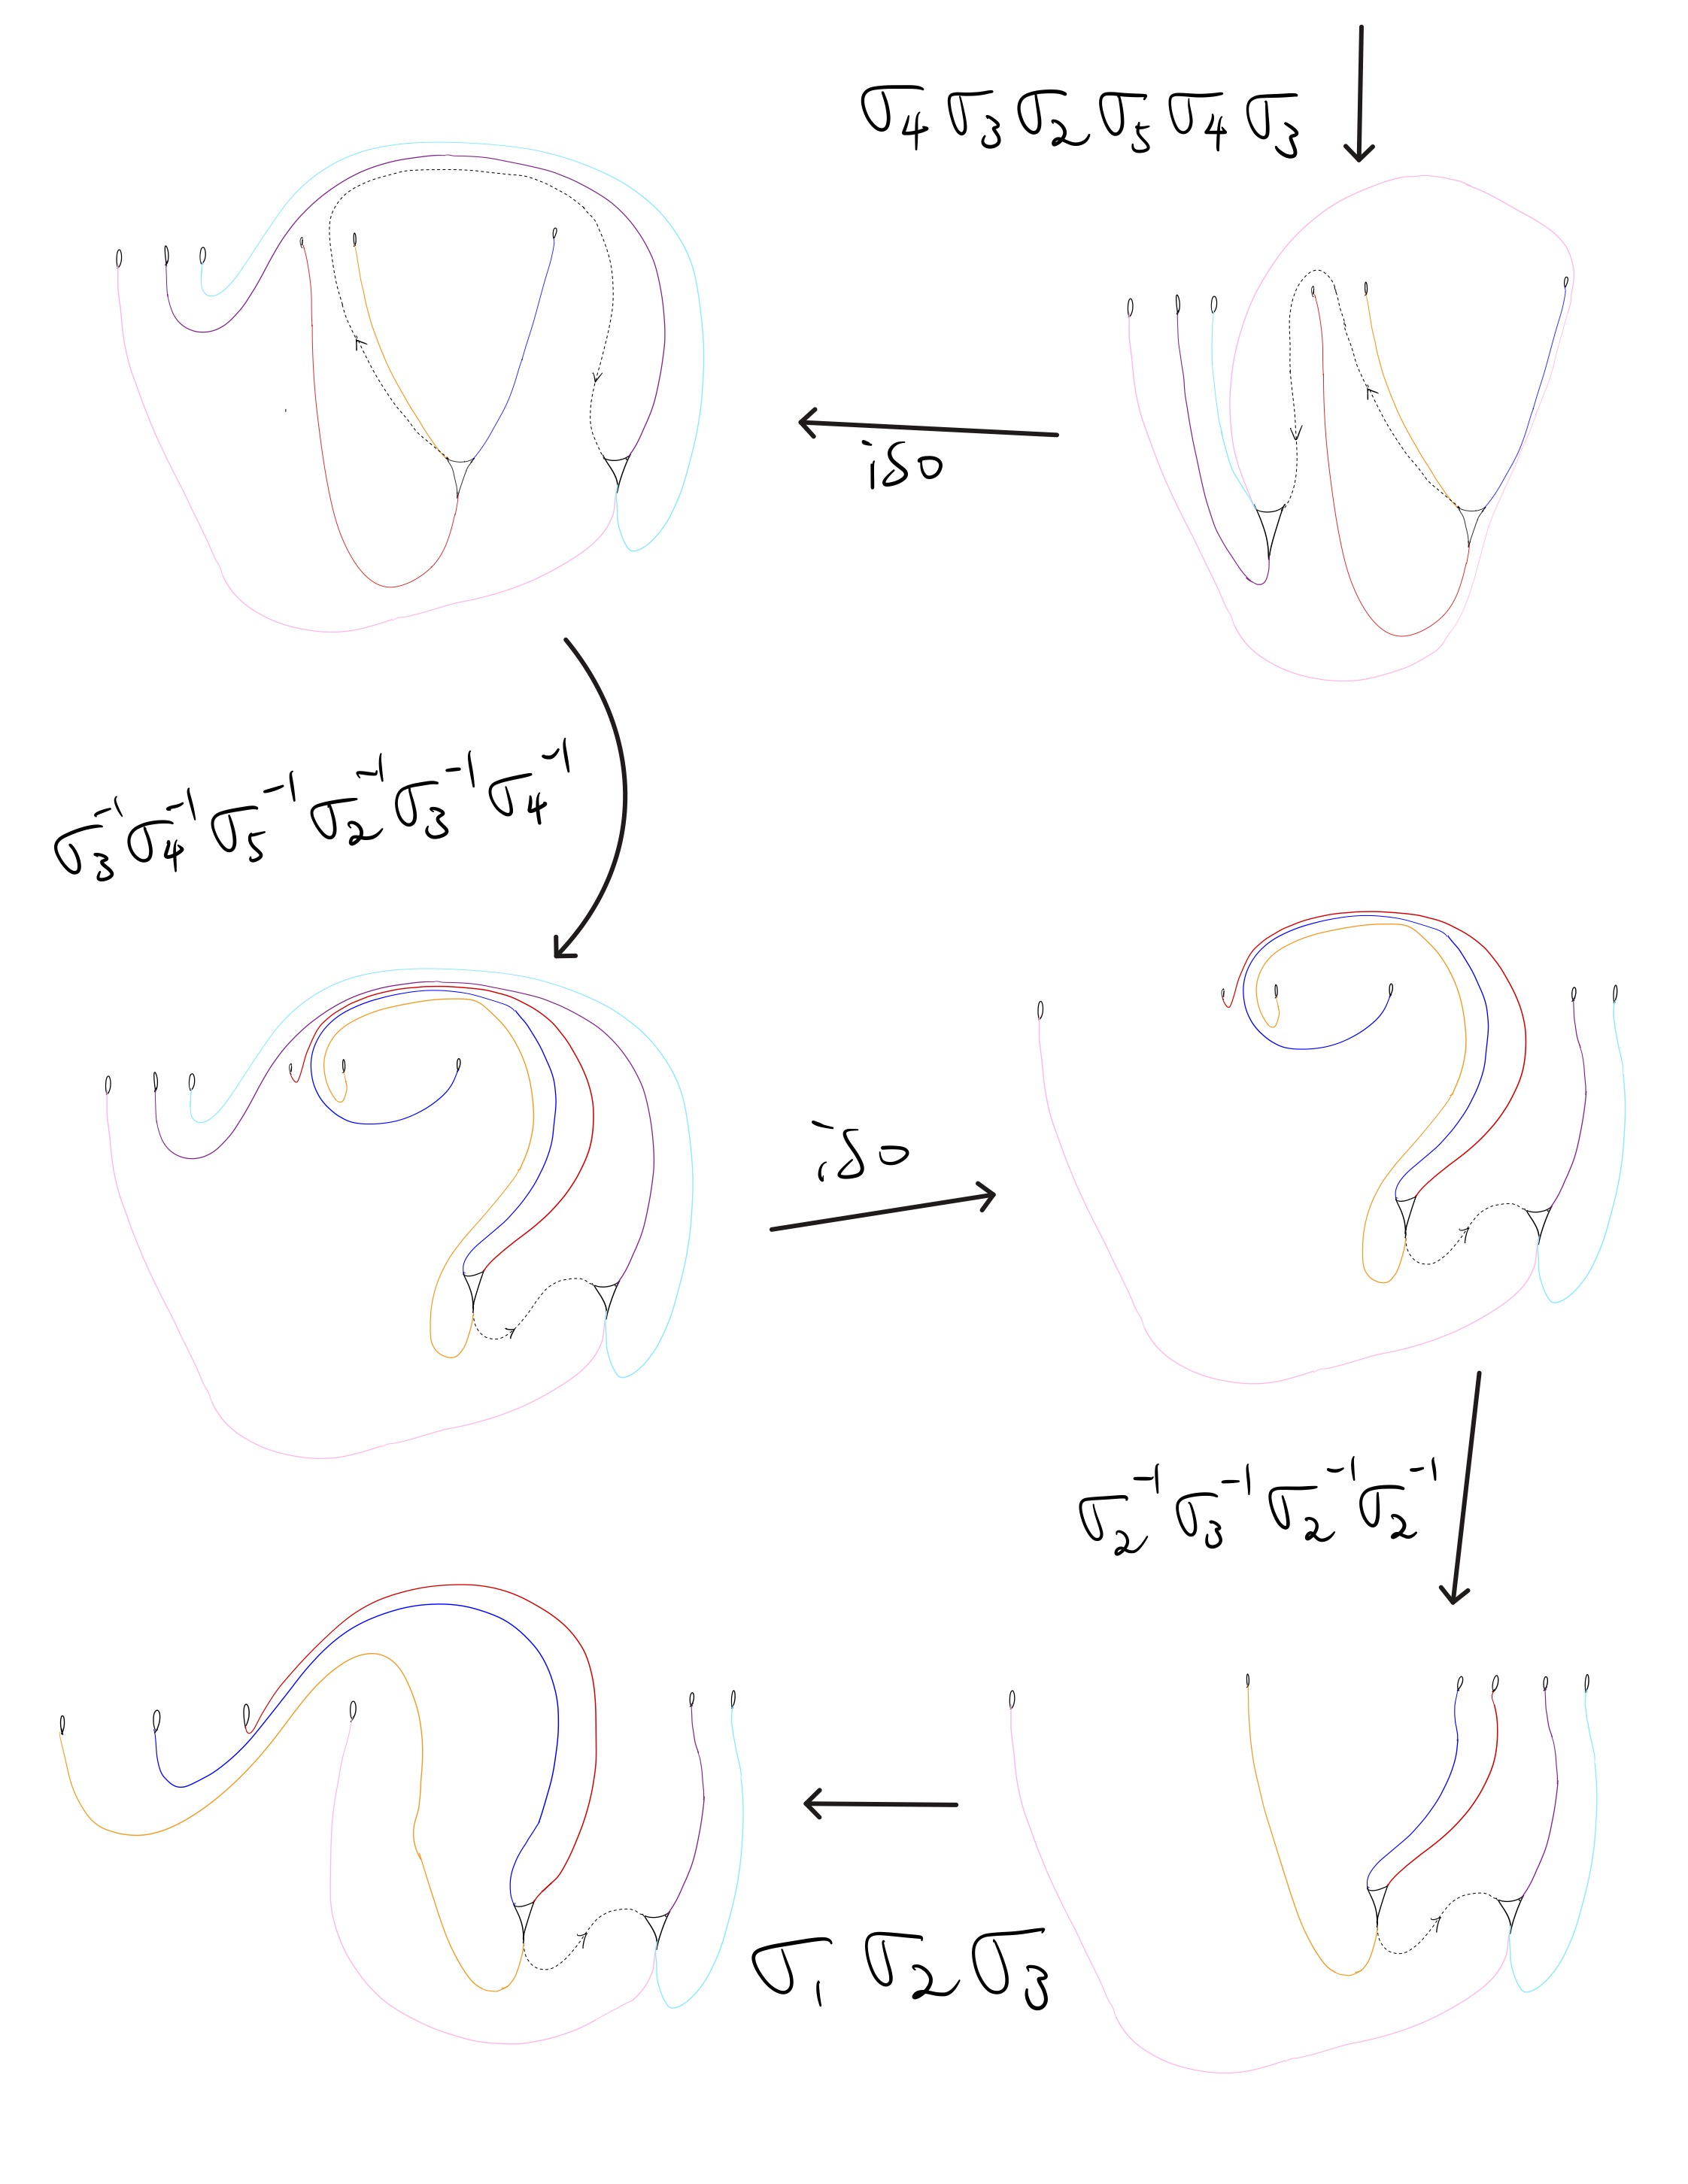
\includegraphics[width=\linewidth, height=0.45\textheight, keepaspectratio]{figures_braid/figures_track_1/Track 1 Braid 8 Panorama-3.jpg}
    \caption{This sequence shows the inverse of the braid $b_8^1$ carries Train Track Candidate Family 8.}
    \label{fig:track1_braid_b1_8}
\end{figure*}

\clearpage

\section{Candidate Family 9 (Pristine)}\label{sec:track1_pristine}
Train Track Map Candidate Family 9 of Track 1 is shown in Figure \ref{fig:track1_braid_b1_9_map}. See \ref{Pristine} for details.

\begin{figure*}[ht]
    \centering
    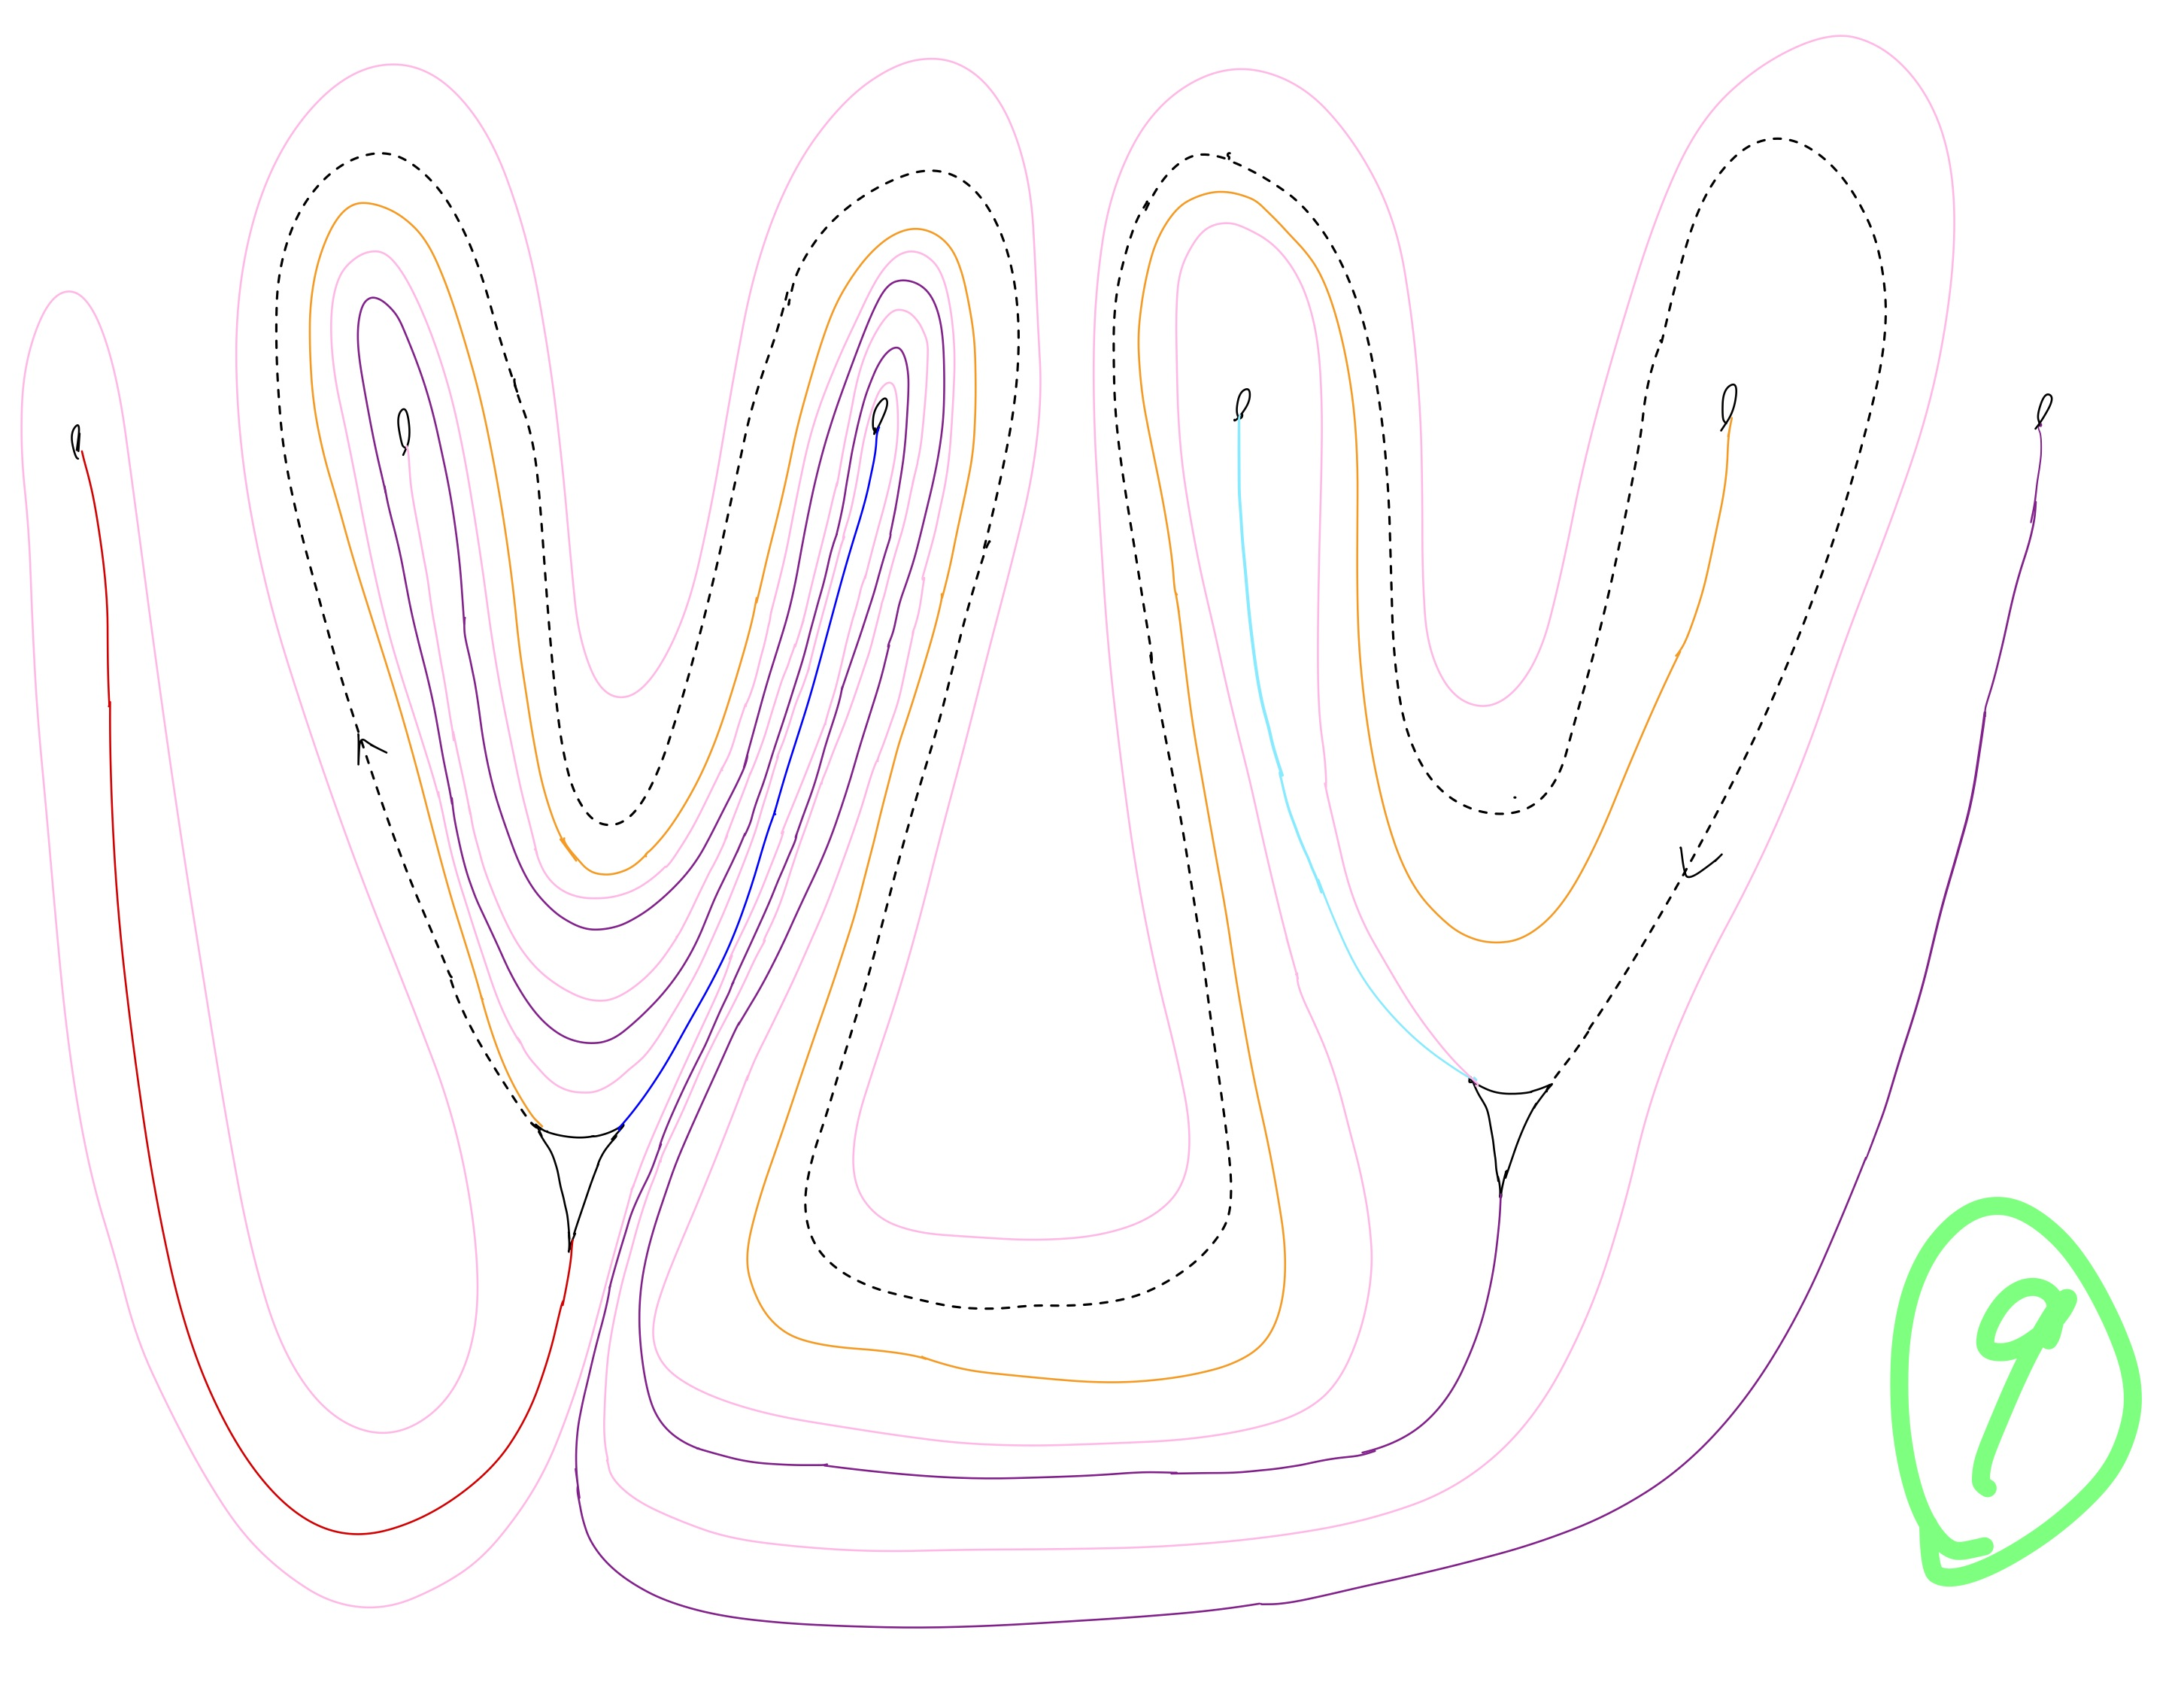
\includegraphics[width=\linewidth, height=0.45\textheight, keepaspectratio]{figures_braid/figures_track_1/Track 1 Braid 9 Pristine-1.jpg}
    \caption{Train Track Map Candidate Family 9 (Pristine) of Track 1.}
    \label{fig:track1_braid_b1_9_map}
\end{figure*}

The inverse of the following braid carries this family of train track maps:
\[
b_9^1 = \sigma_{4} \sigma_{3} \sigma_{2} \sigma_{3}^{-1} \sigma_{4} \sigma_{4} \sigma_{3} \sigma_{2} \sigma_{1} \sigma_{2}^{-1} \sigma_{3}^{-1} \sigma_{2}^{-1} \sigma_{2}^{-1} \sigma_{1} \sigma_{2} \sigma_{3} \sigma_{5} \sigma_{4} \sigma_{5}
\]

This is shown in Figure \ref{fig:track1_braid_b1_9}.

\begin{figure*}[p]
    \centering
    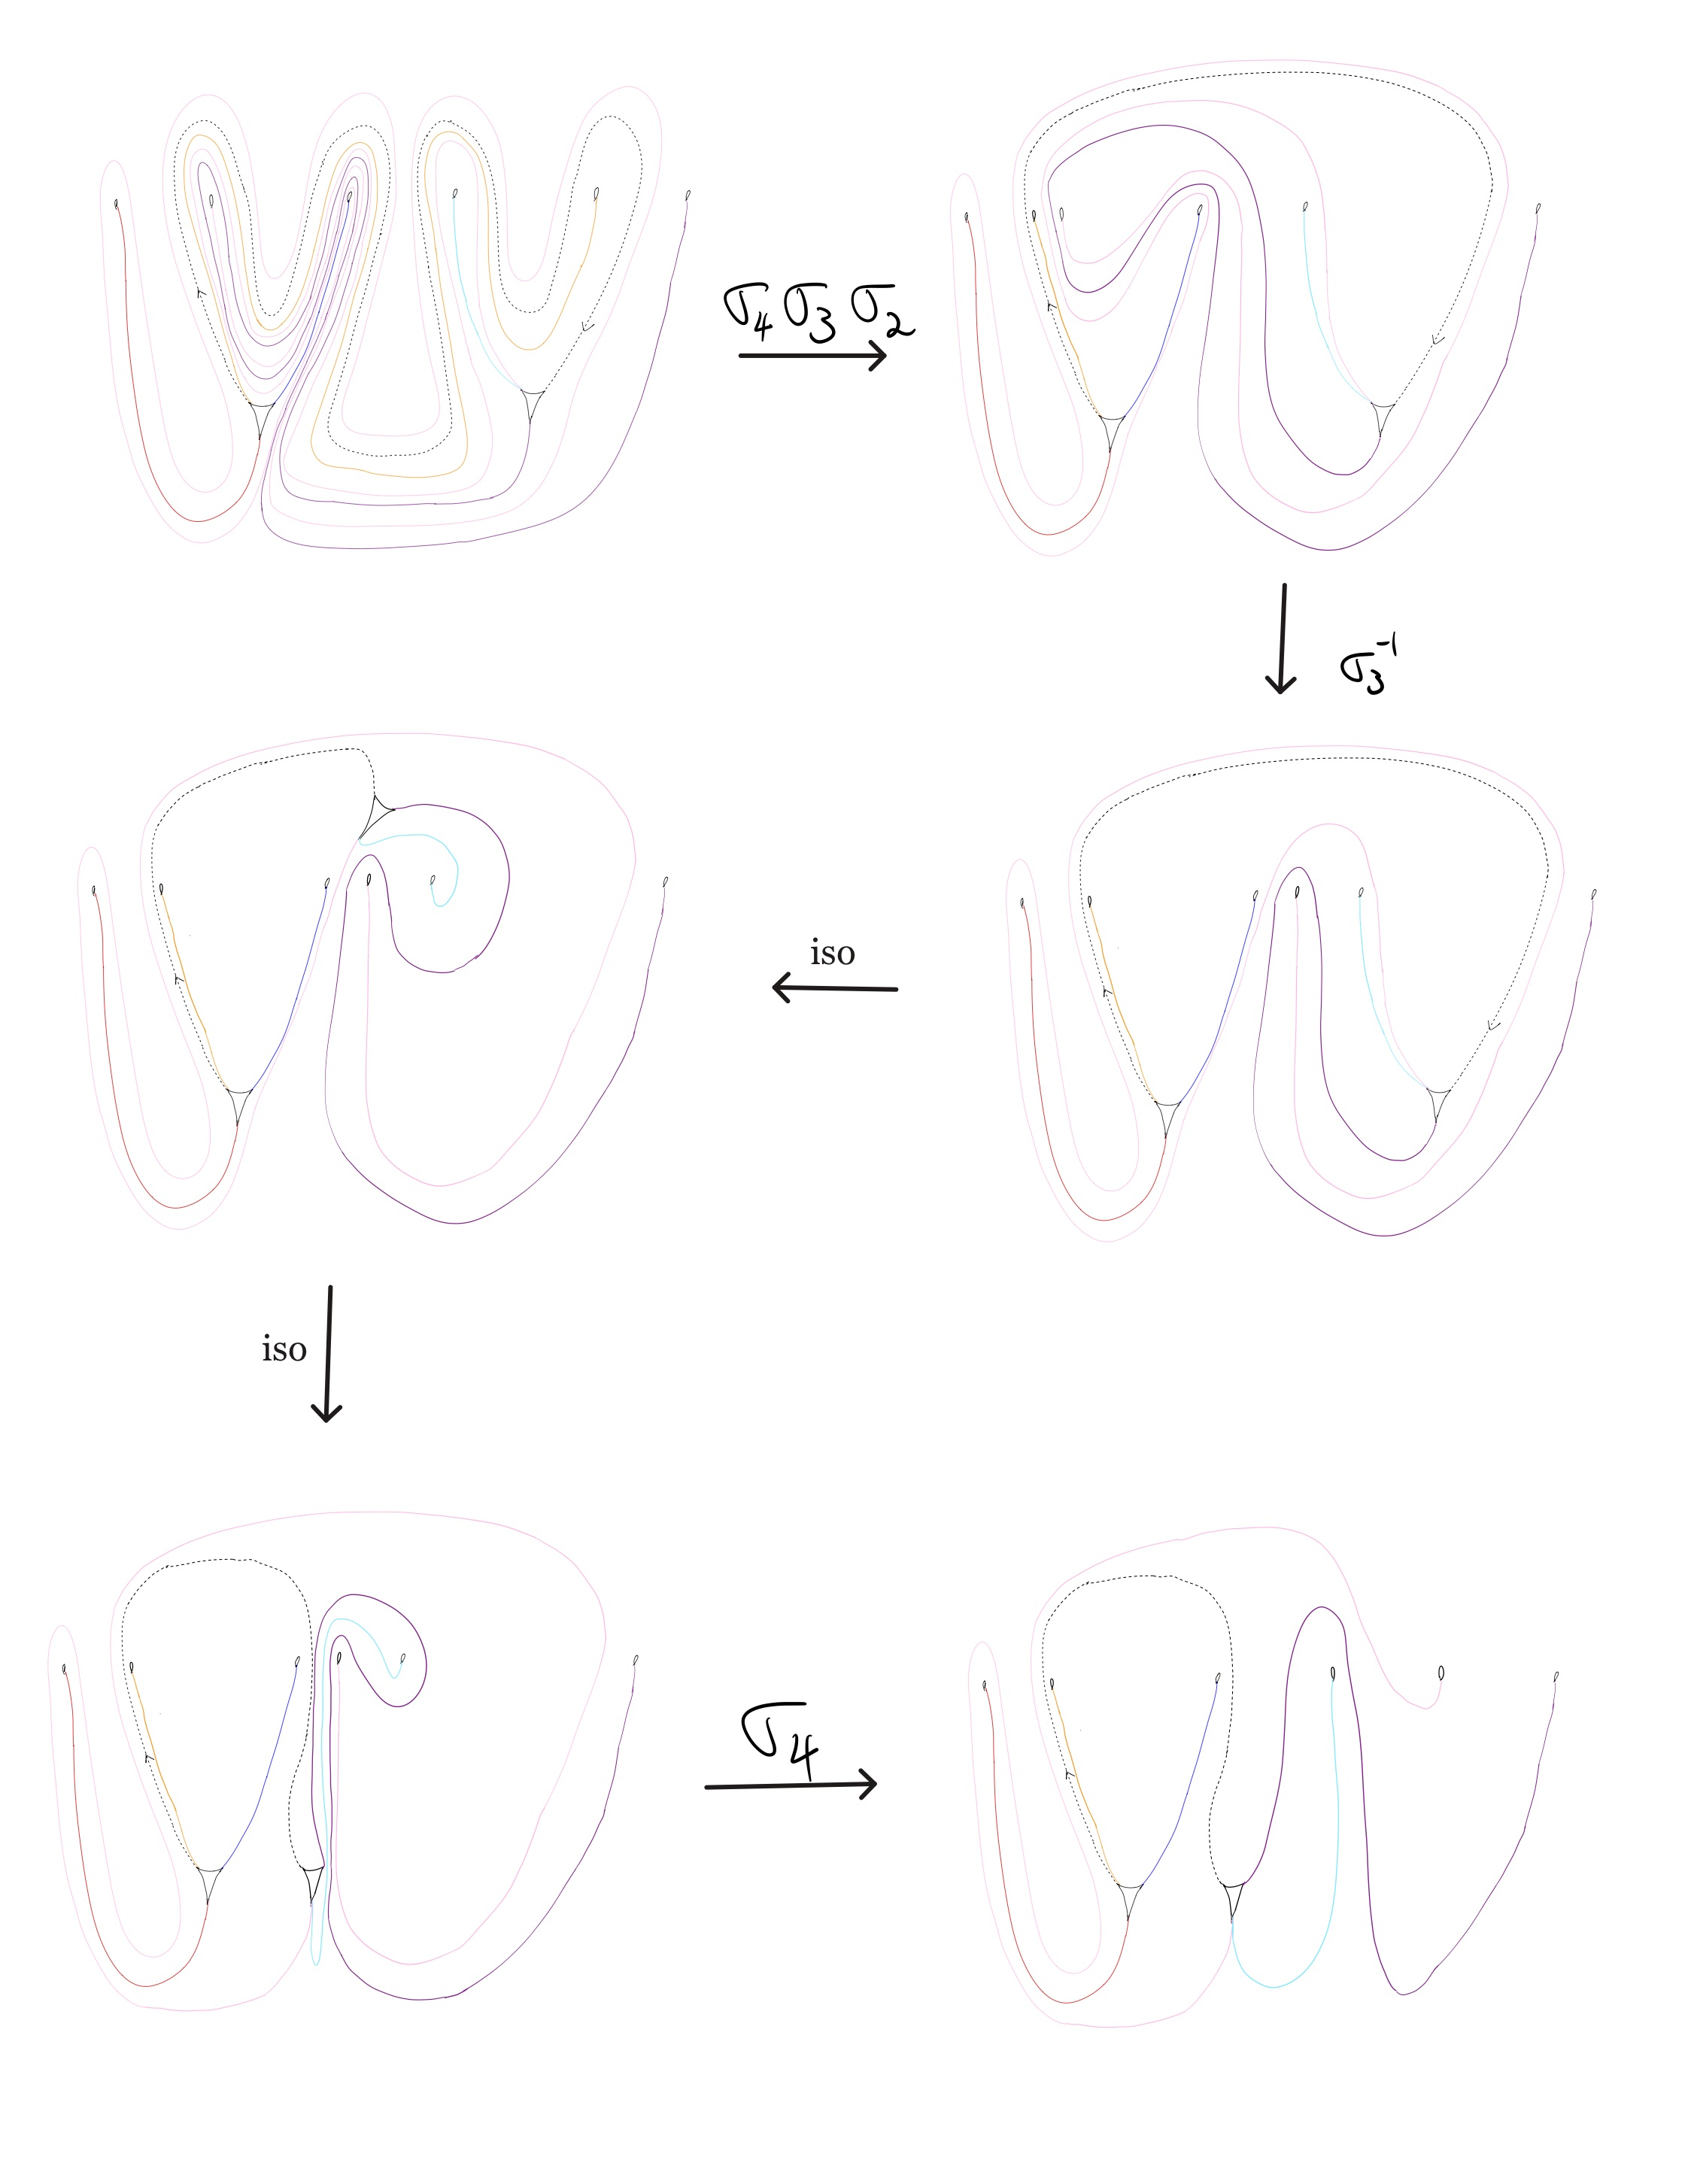
\includegraphics[width=\linewidth, height=0.45\textheight, keepaspectratio]{figures_braid/figures_track_1/Track 1 Braid 9 Pristine-2.jpg}\\
    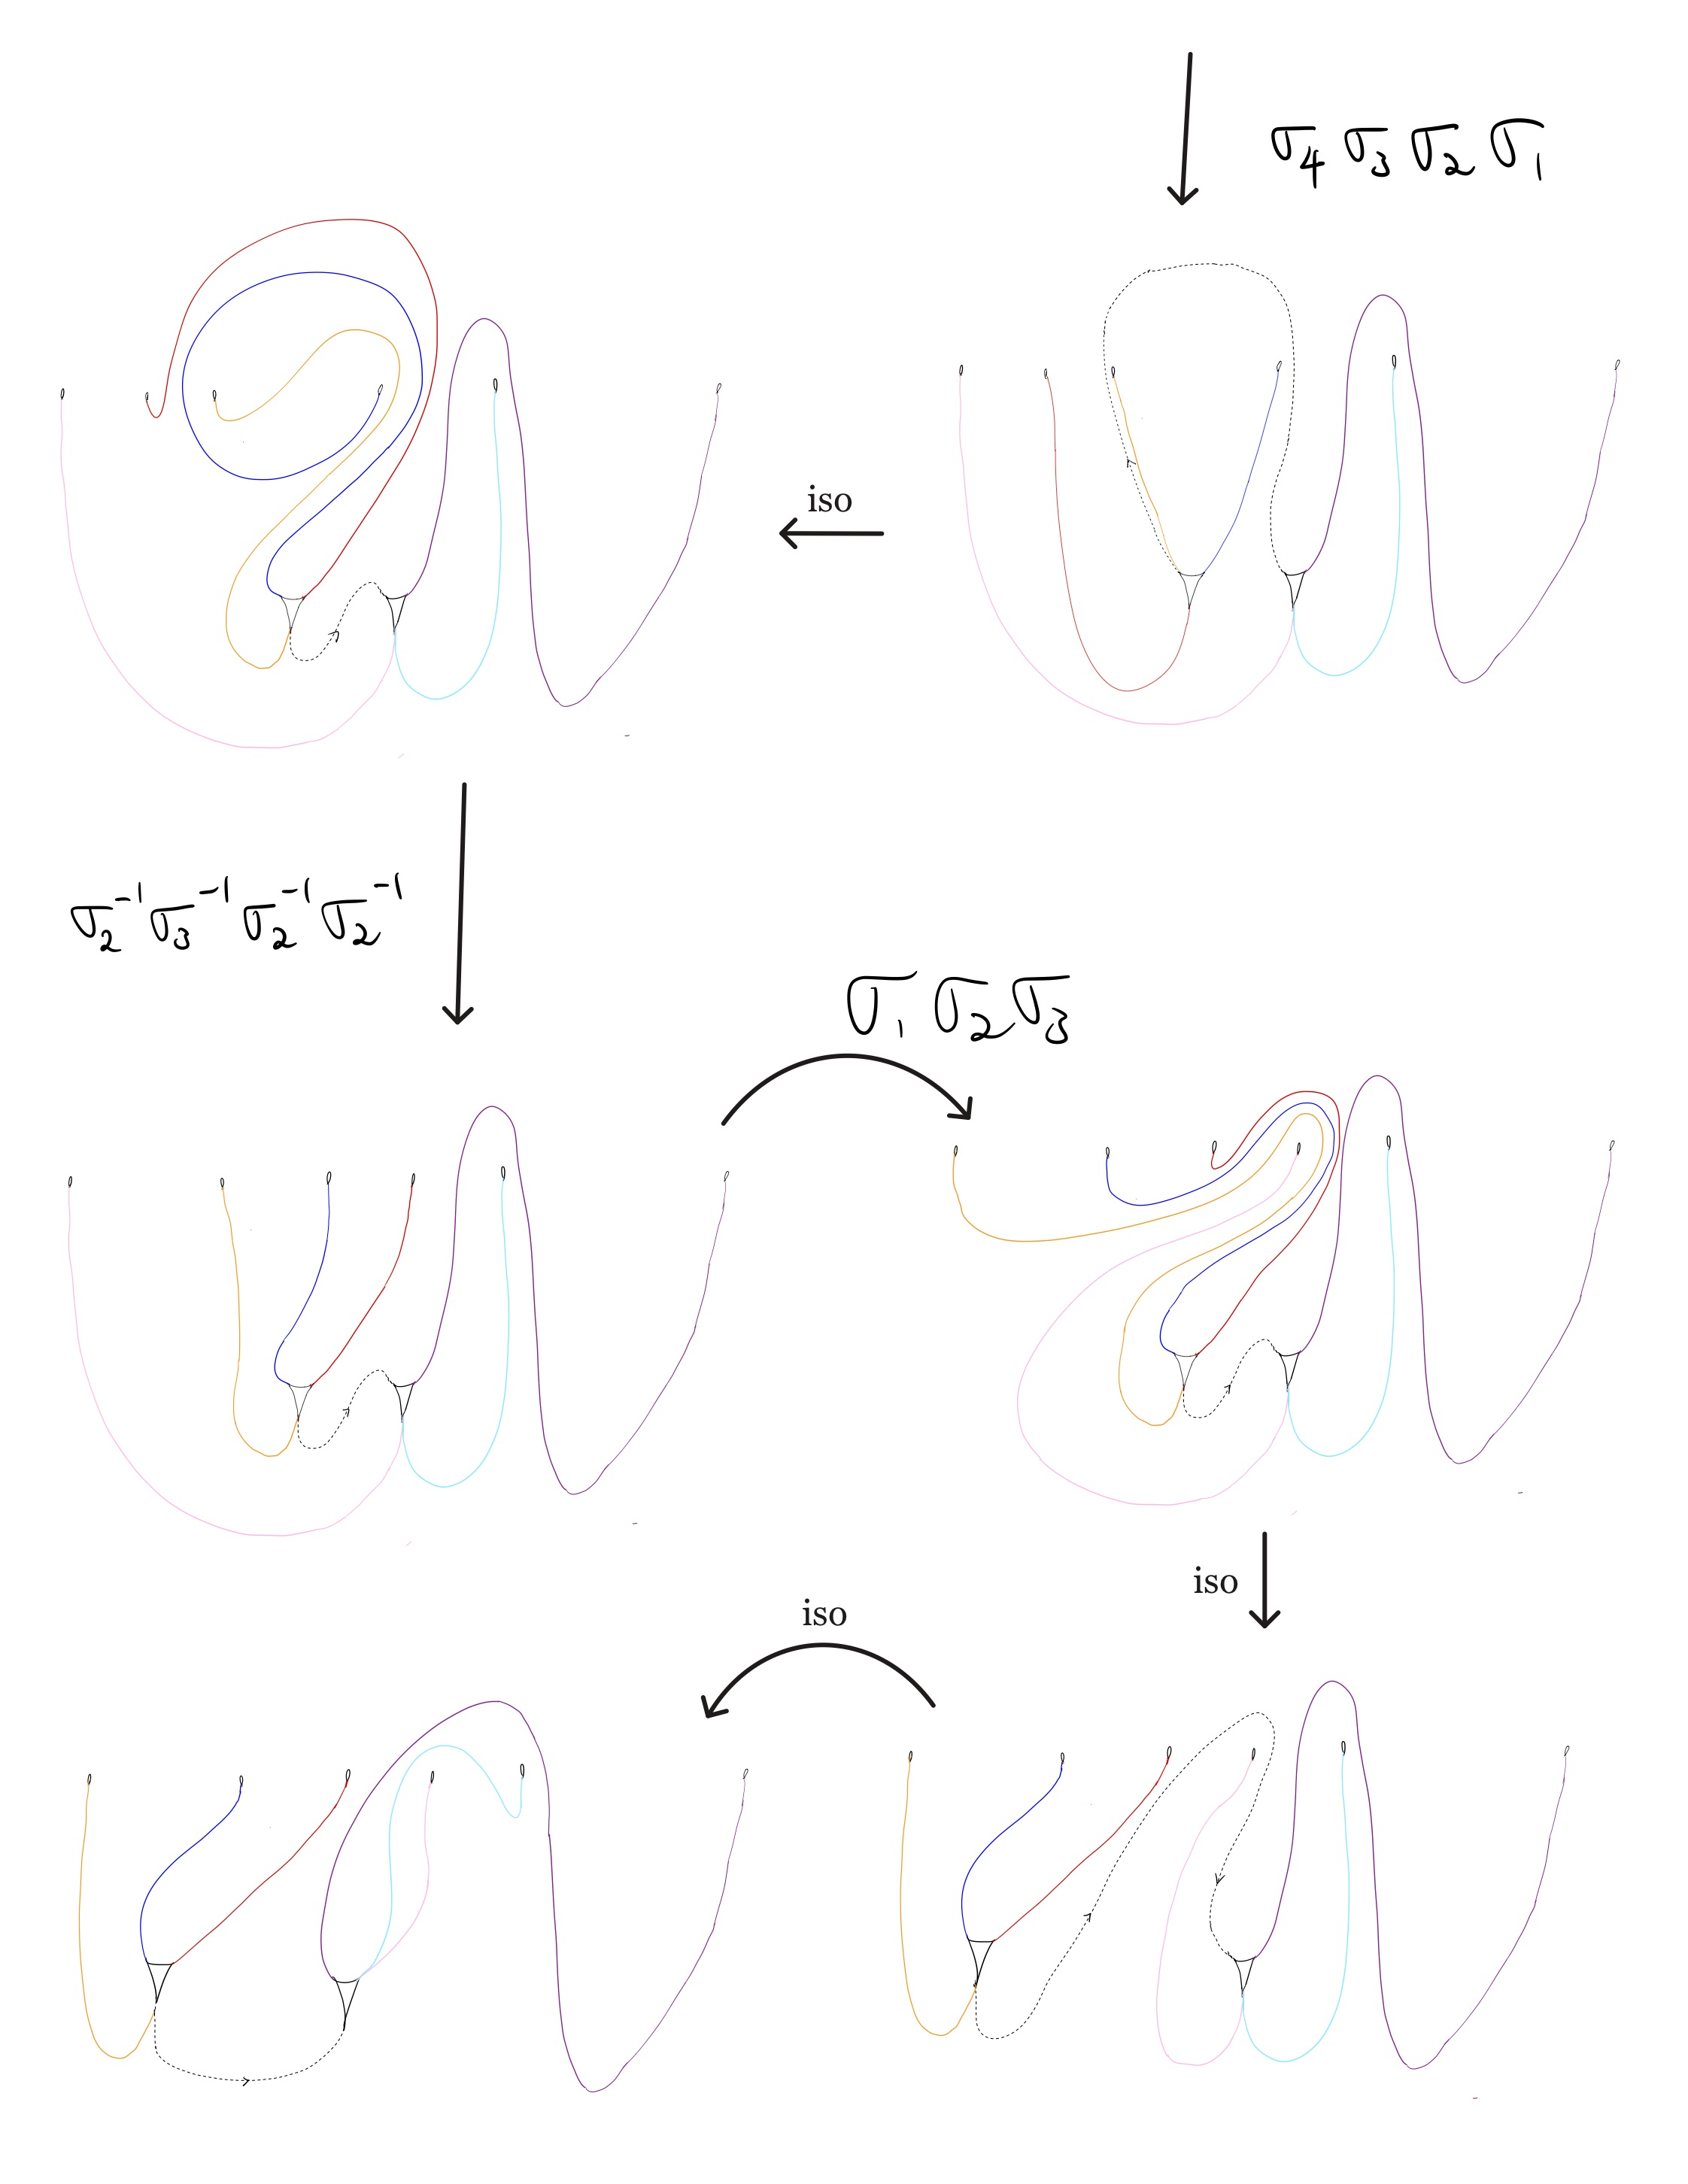
\includegraphics[width=\linewidth, height=0.45\textheight, keepaspectratio]{figures_braid/figures_track_1/Track 1 Braid 9 Pristine-3.jpg}
    \caption{This sequence shows the inverse of the braid $b_9^1$ carries Train Track Candidate Family 9.}
    \label{fig:track1_braid_b1_9}
\end{figure*}

\clearpage

\section{Candidate Family 10 (Gingham)}\label{sec:track1_gingham}
Train Track Map Candidate Family 10 of Track 1 is shown in Figure \ref{fig:track1_braid_b1_10_map}. See \ref{Gingham} for details.

\begin{figure*}[ht]
    \centering
    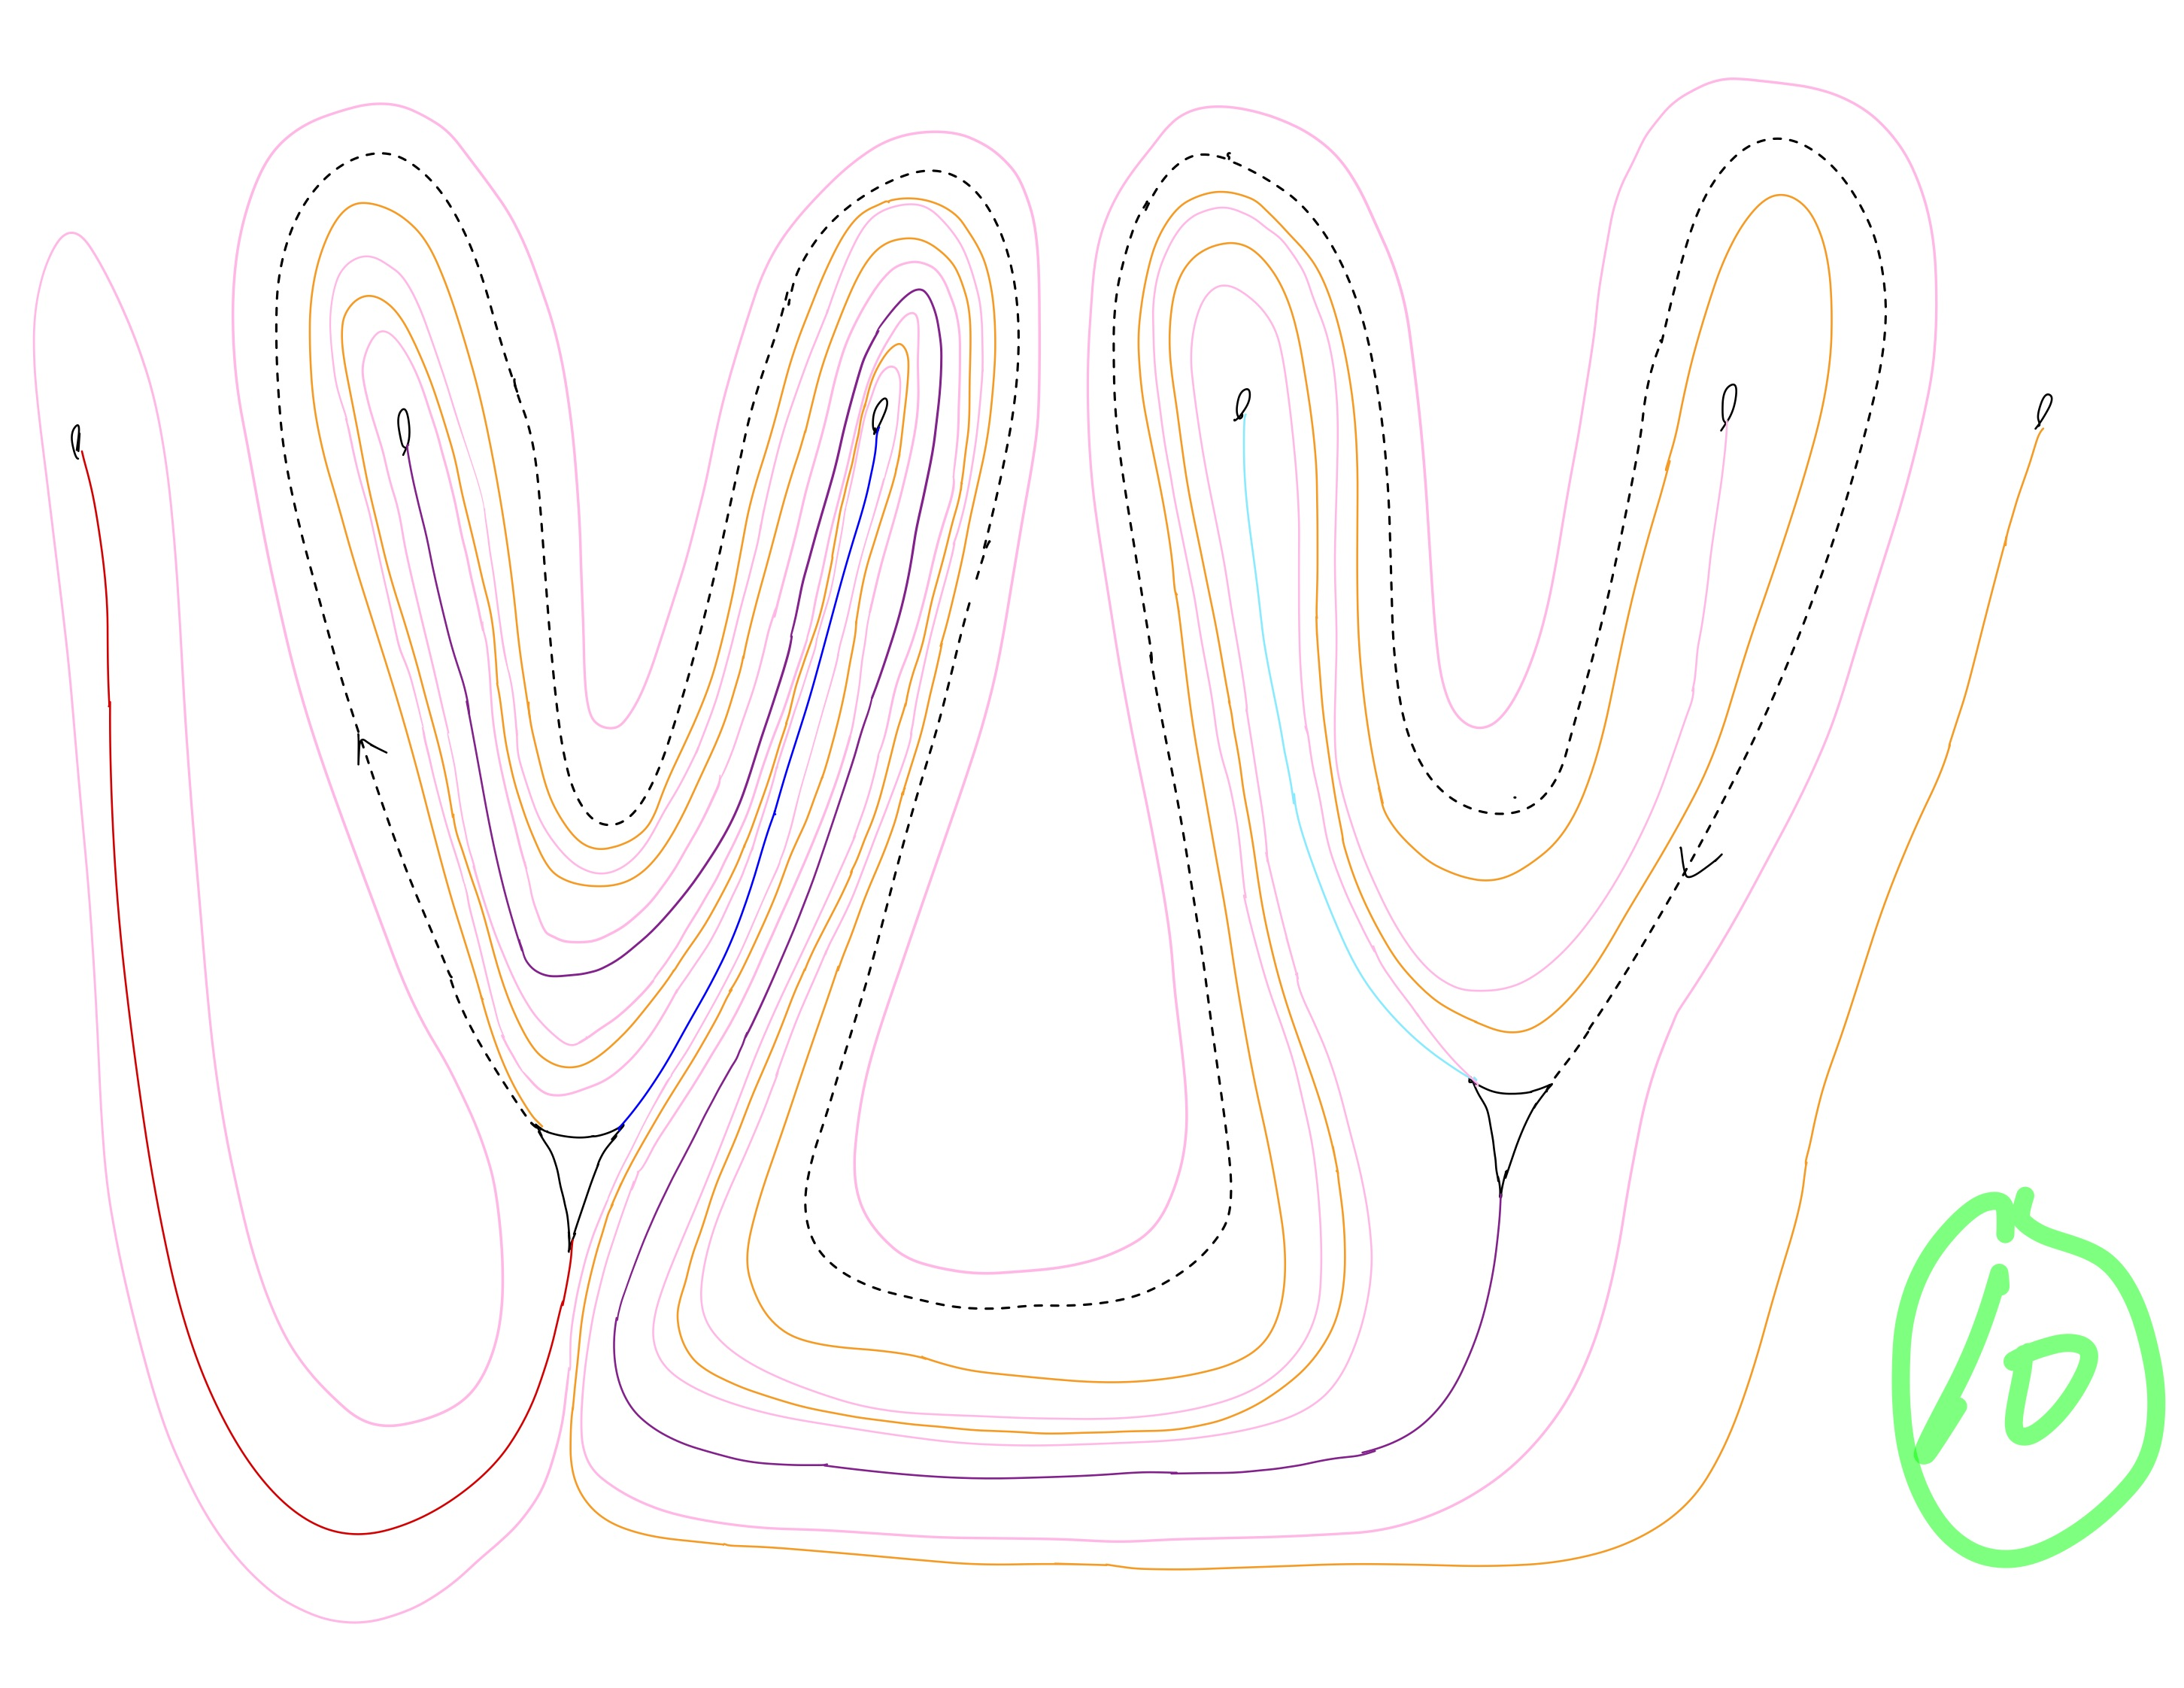
\includegraphics[width=\linewidth, height=0.45\textheight, keepaspectratio]{figures_braid/figures_track_1/Track 1 Braid 10 Gingham-1.jpg}
    \caption{Train Track Map Candidate Family 10 (Gingham) of Track 1.}
    \label{fig:track1_braid_b1_10_map}
\end{figure*}

The inverse of the following braid carries this family of train track maps:
\[
b_{10}^1 = \sigma_{4} \sigma_{3} \sigma_{2} \sigma_{3}^{-1} \sigma_{4} \sigma_{4} \sigma_{3} \sigma_{2} \sigma_{1} \sigma_{4} \sigma_{3} \sigma_{2} \sigma_{5} \sigma_{4} \sigma_{5}^{-1} \sigma_{5}^{-1} \sigma_{4}^{-1} \sigma_{3}^{-1} \sigma_{2}^{-1} \sigma_{1}^{-1} \sigma_{1}^{-1} \sigma_{2}^{-1} \sigma_{4} \sigma_{5} \circ J \circ \Lambda_6
\]

This is shown in Figure \ref{fig:track1_braid_b1_10}.

\begin{figure*}[p]
    \centering
    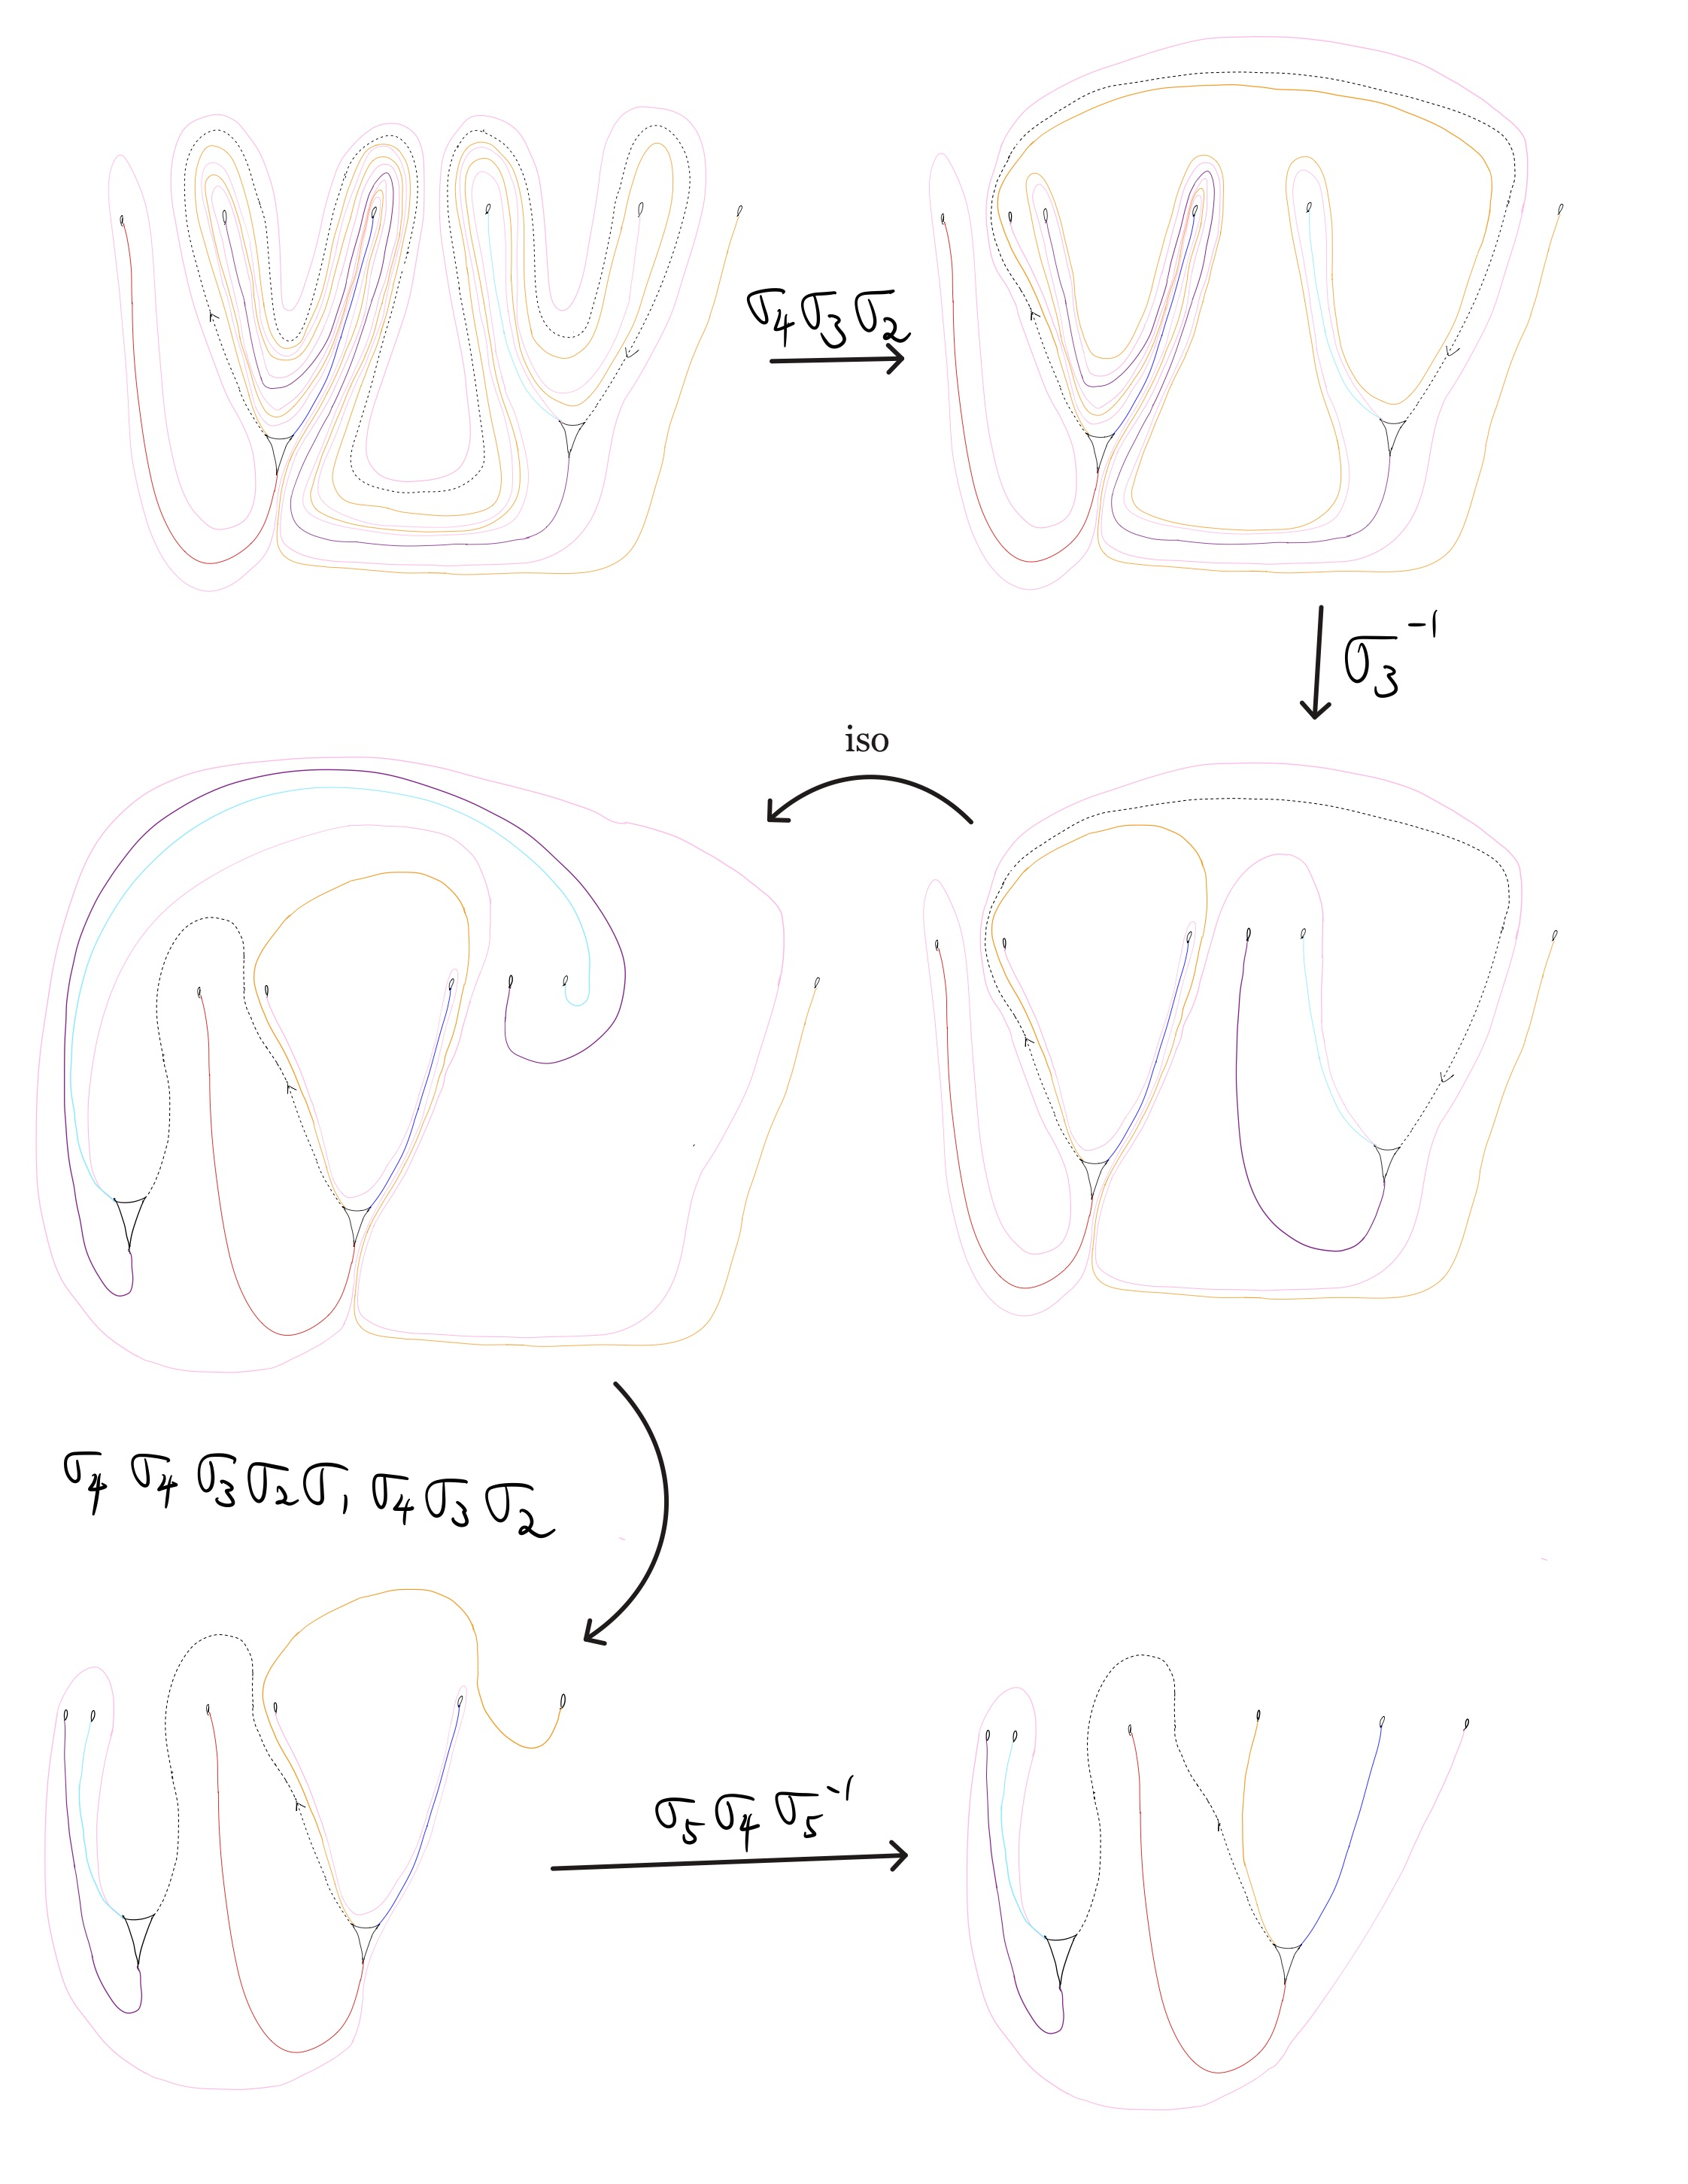
\includegraphics[width=\linewidth, height=0.45\textheight, keepaspectratio]{figures_braid/figures_track_1/Track 1 Braid 10 Gingham-2.jpg}\\
    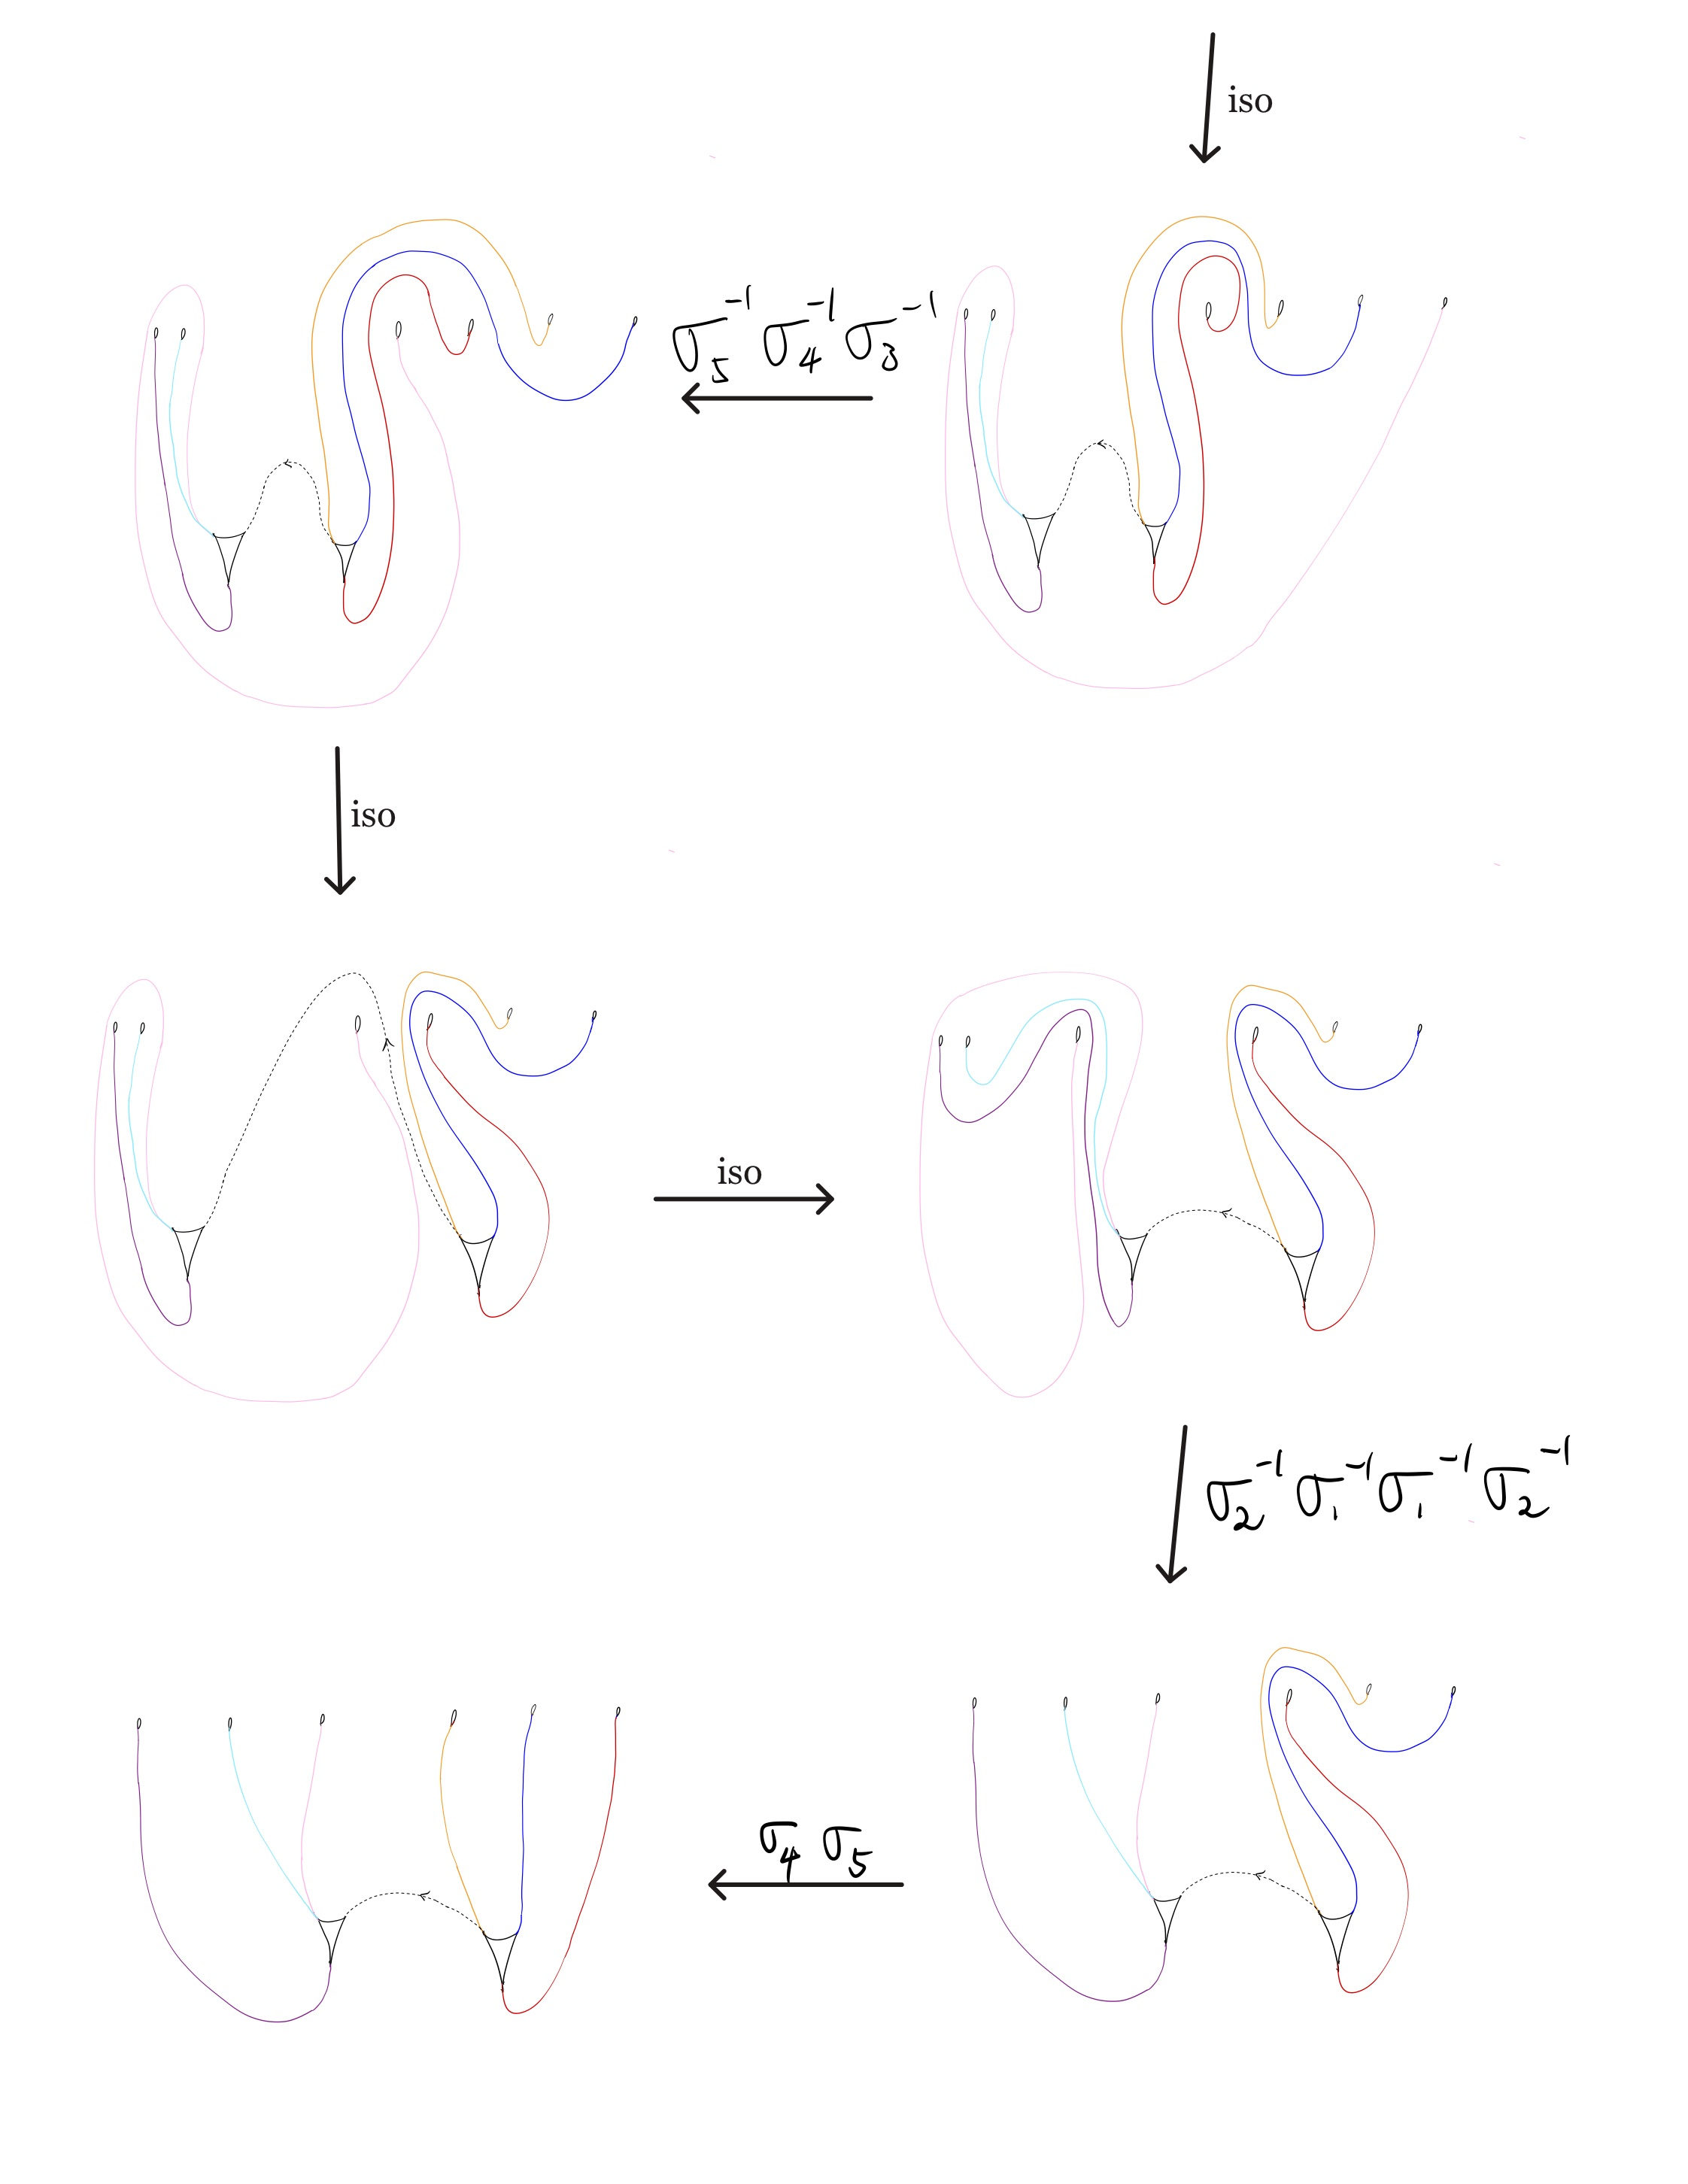
\includegraphics[width=\linewidth, height=0.45\textheight, keepaspectratio]{figures_braid/figures_track_1/Track 1 Braid 10 Gingham-3.jpg}
    \caption{This sequence shows the inverse of the braid $b_{10}^1$ carries Train Track Candidate Family 10.}
    \label{fig:track1_braid_b1_10}
\end{figure*}

\clearpage

\section{Candidate Family 11 (Dossier)}\label{sec:track1_dossier}
Train Track Map Candidate Family 11 of Track 1 is shown in Figure \ref{fig:track1_braid_b1_11_map}. See \ref{Dossier} for details.

\begin{figure*}[ht]
    \centering
    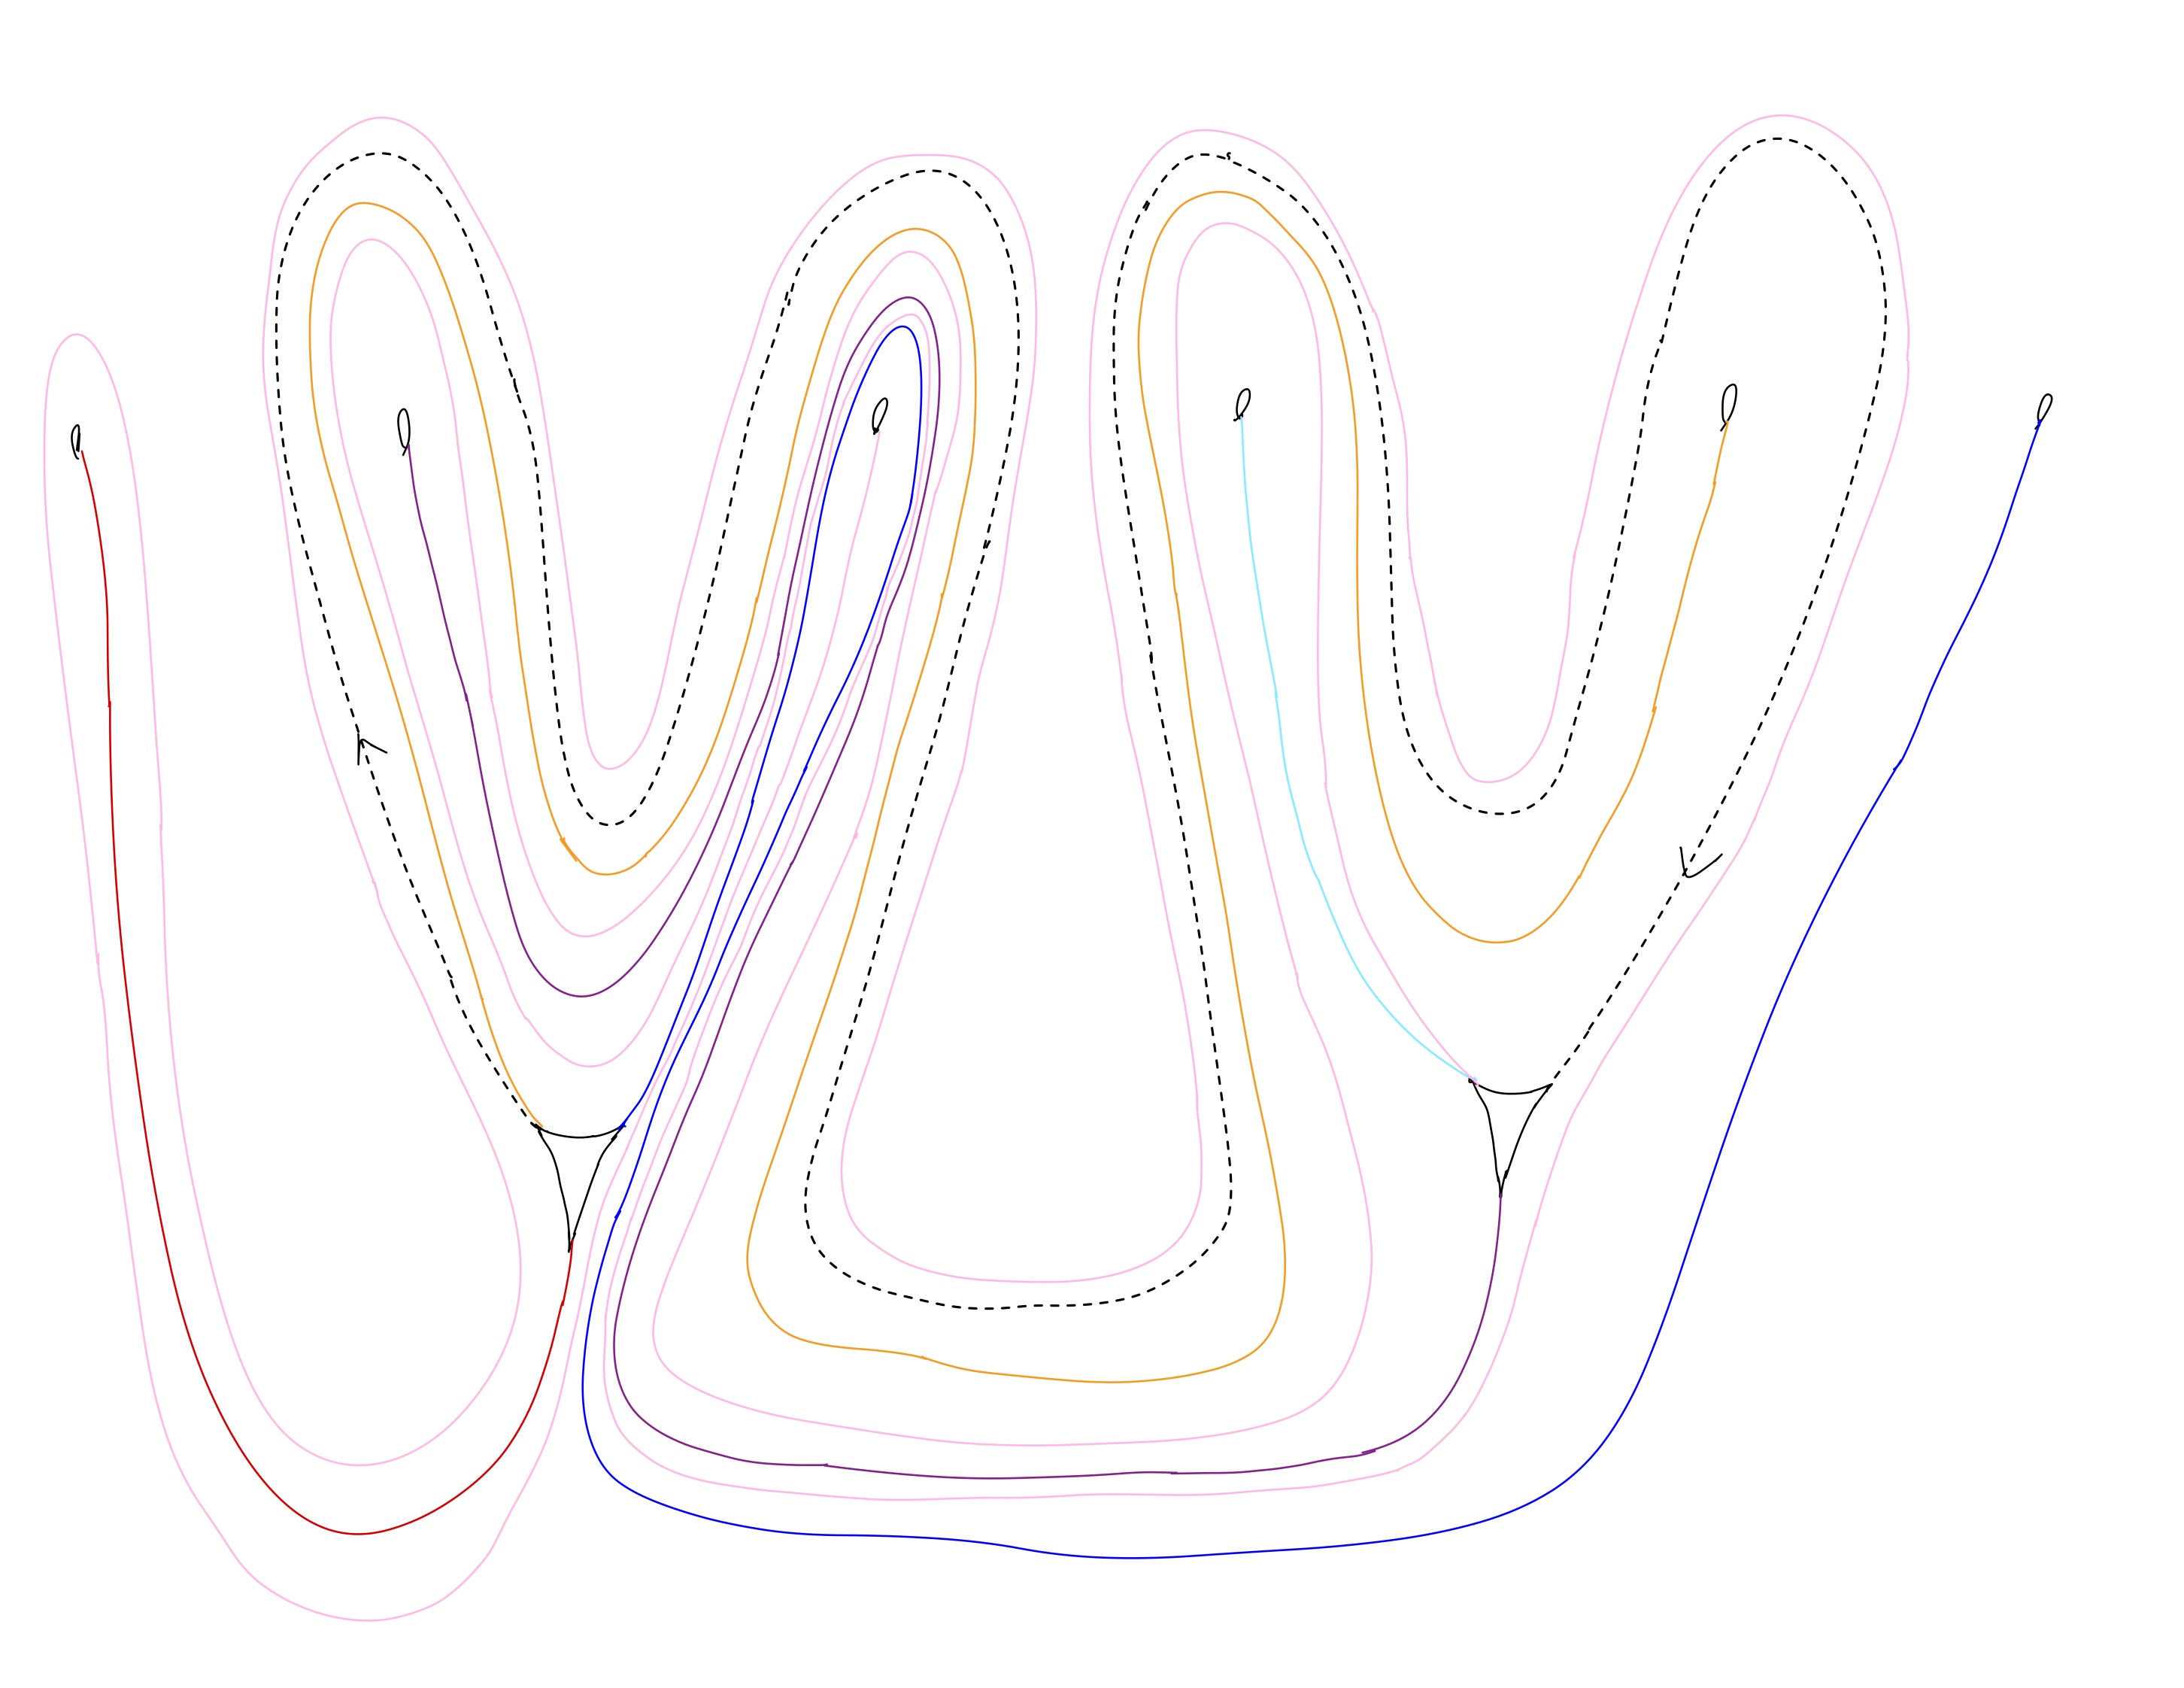
\includegraphics[width=\linewidth, height=0.45\textheight, keepaspectratio]{figures_braid/figures_track_1/Track 1 Braid 11 Dossier-1.jpg}
    \caption{Train Track Map Candidate Family 11 (Dossier) of Track 1.}
    \label{fig:track1_braid_b1_11_map}
\end{figure*}

The inverse of the following braid carries this family of train track maps:
\[
b_{11}^1 = \sigma_{4} \sigma_{3} \sigma_{2} \sigma_{3}^{-1} \sigma_{4} \sigma_{4} \sigma_{3} \sigma_{2} \sigma_{1} \sigma_{4} \sigma_{3} \sigma_{2} \sigma_{4}^{-1} \sigma_{5}^{-1} \sigma_{3}^{-1} \sigma_{2}^{-1} \sigma_{1}^{-1} \sigma_{1}^{-1} \sigma_{2}^{-1} \sigma_{5} \sigma_{4} \sigma_{5} \circ J \circ \Lambda_6
\]

This is shown in Figure \ref{fig:track1_braid_b1_11}.

\begin{figure*}[p]
    \centering
    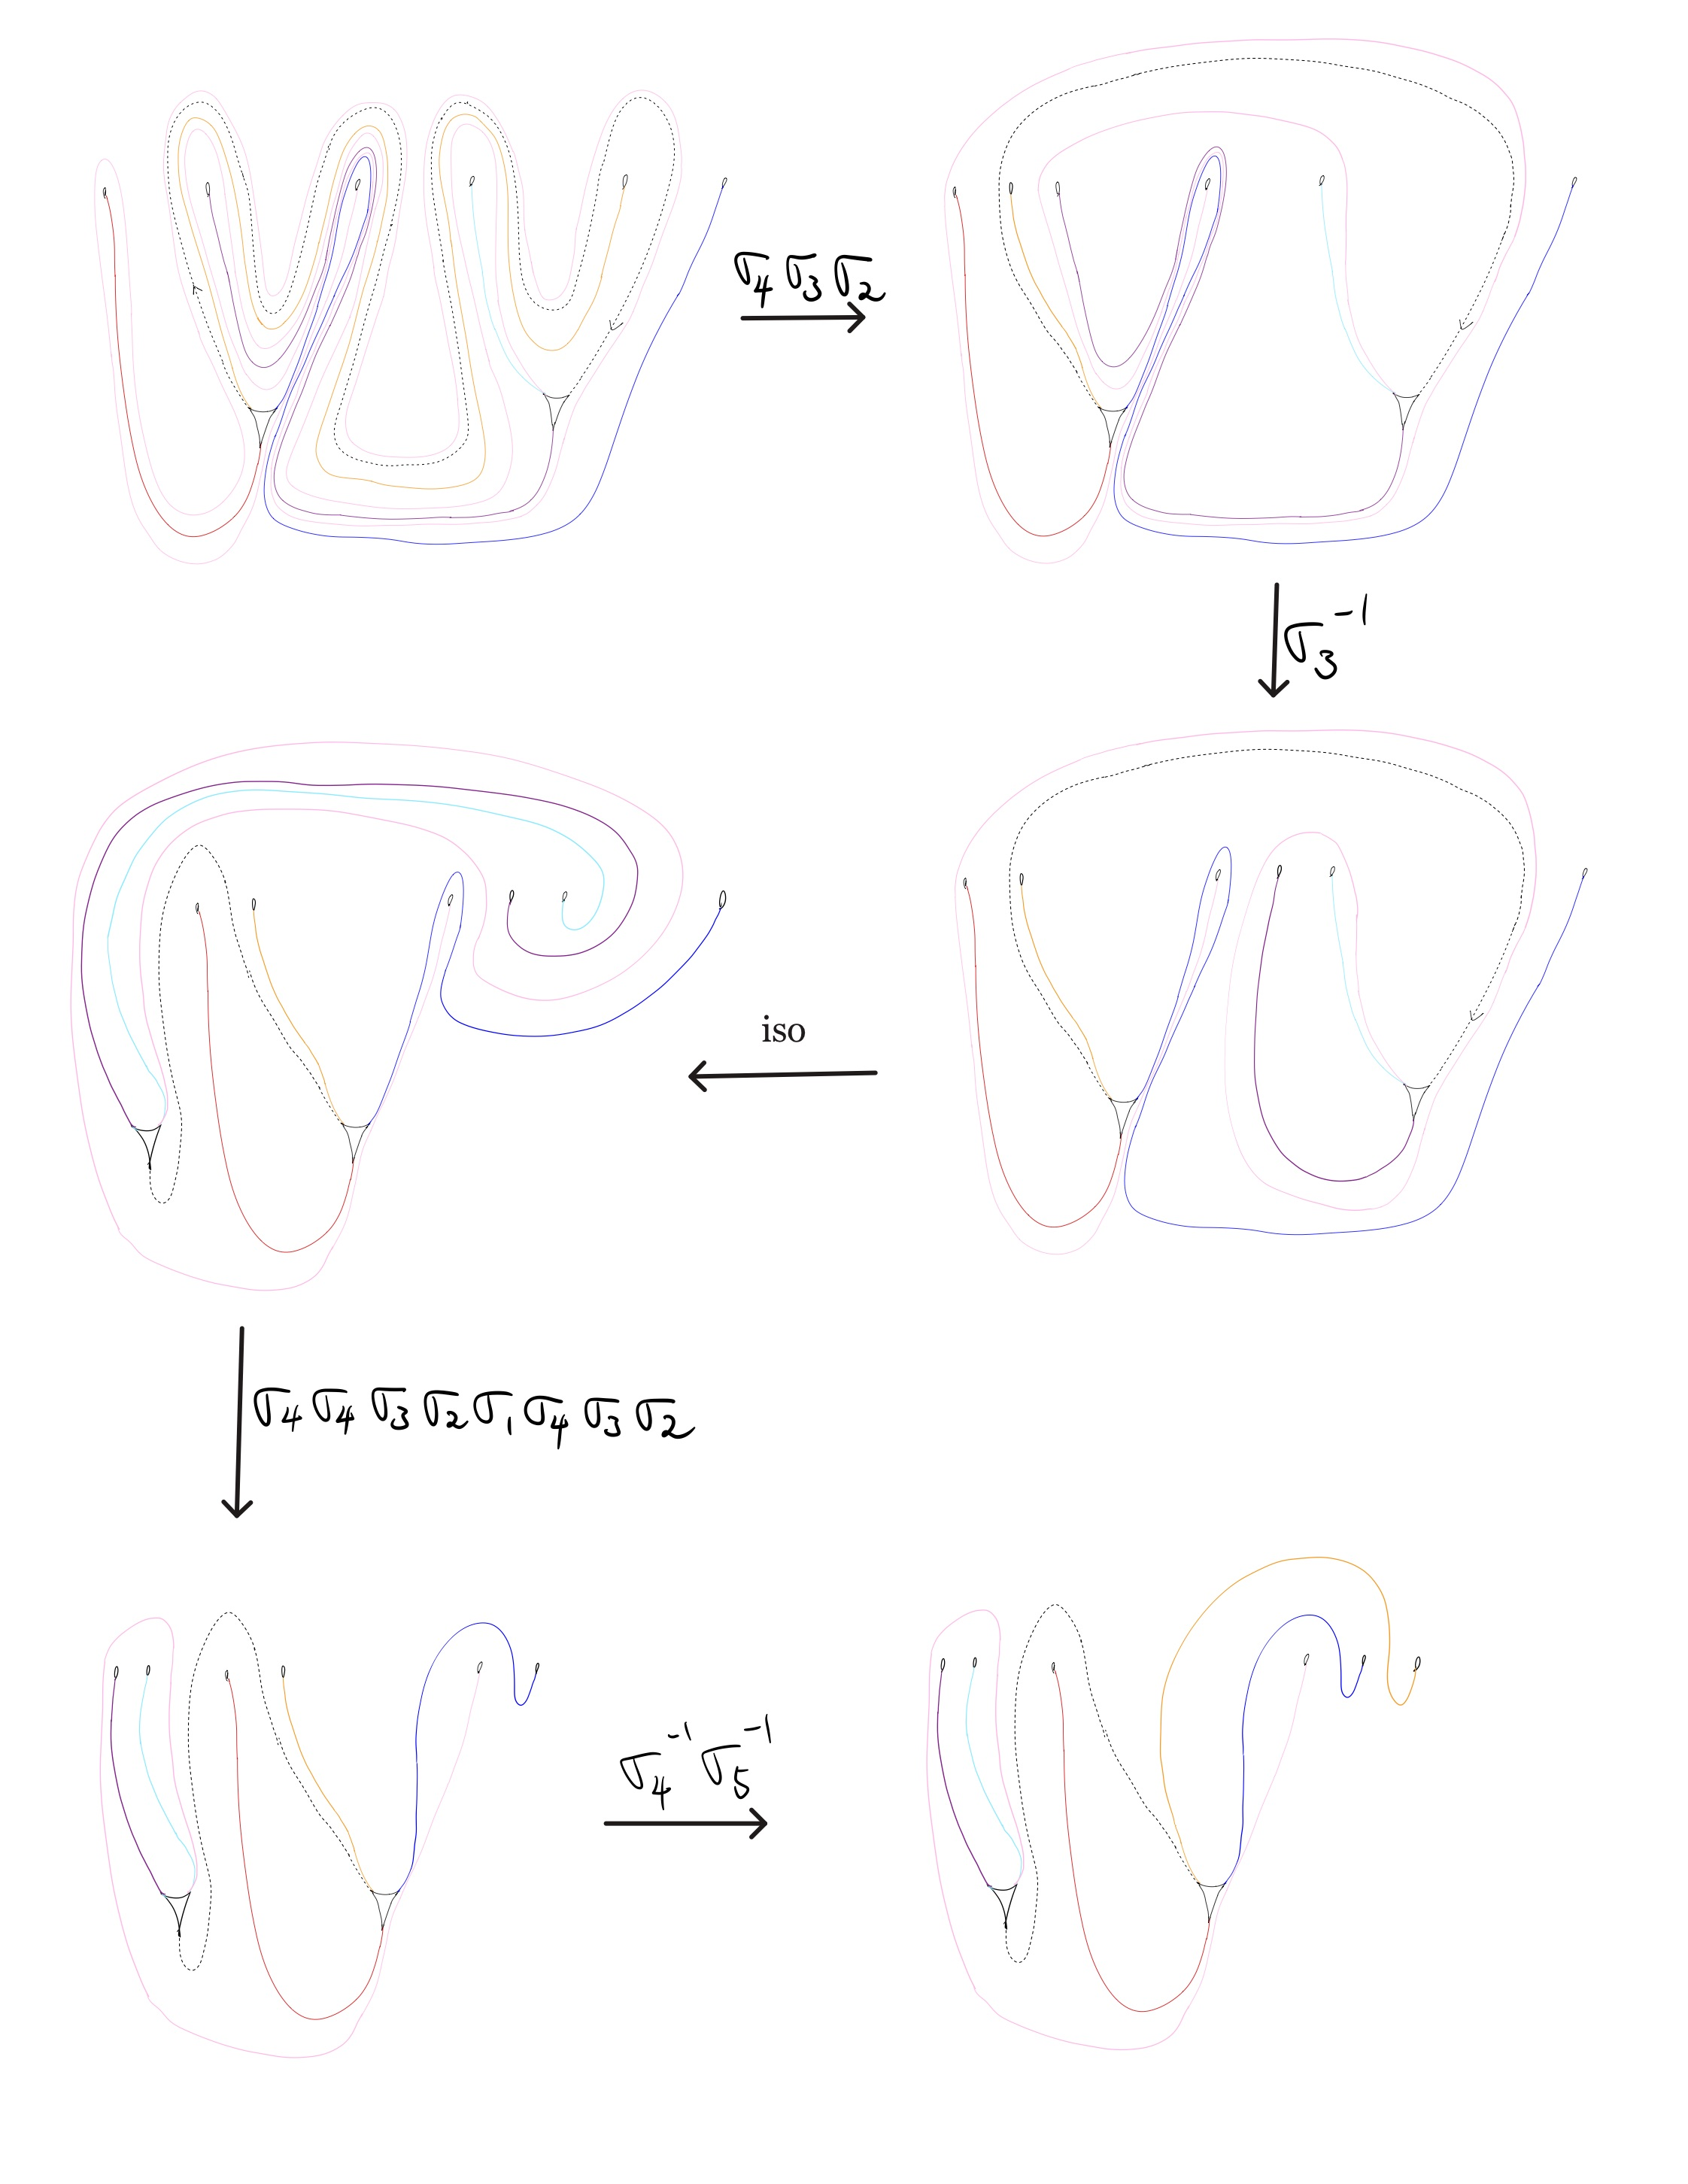
\includegraphics[width=\linewidth, height=0.45\textheight, keepaspectratio]{figures_braid/figures_track_1/Track 1 Braid 11 Dossier-2.jpg}\\
    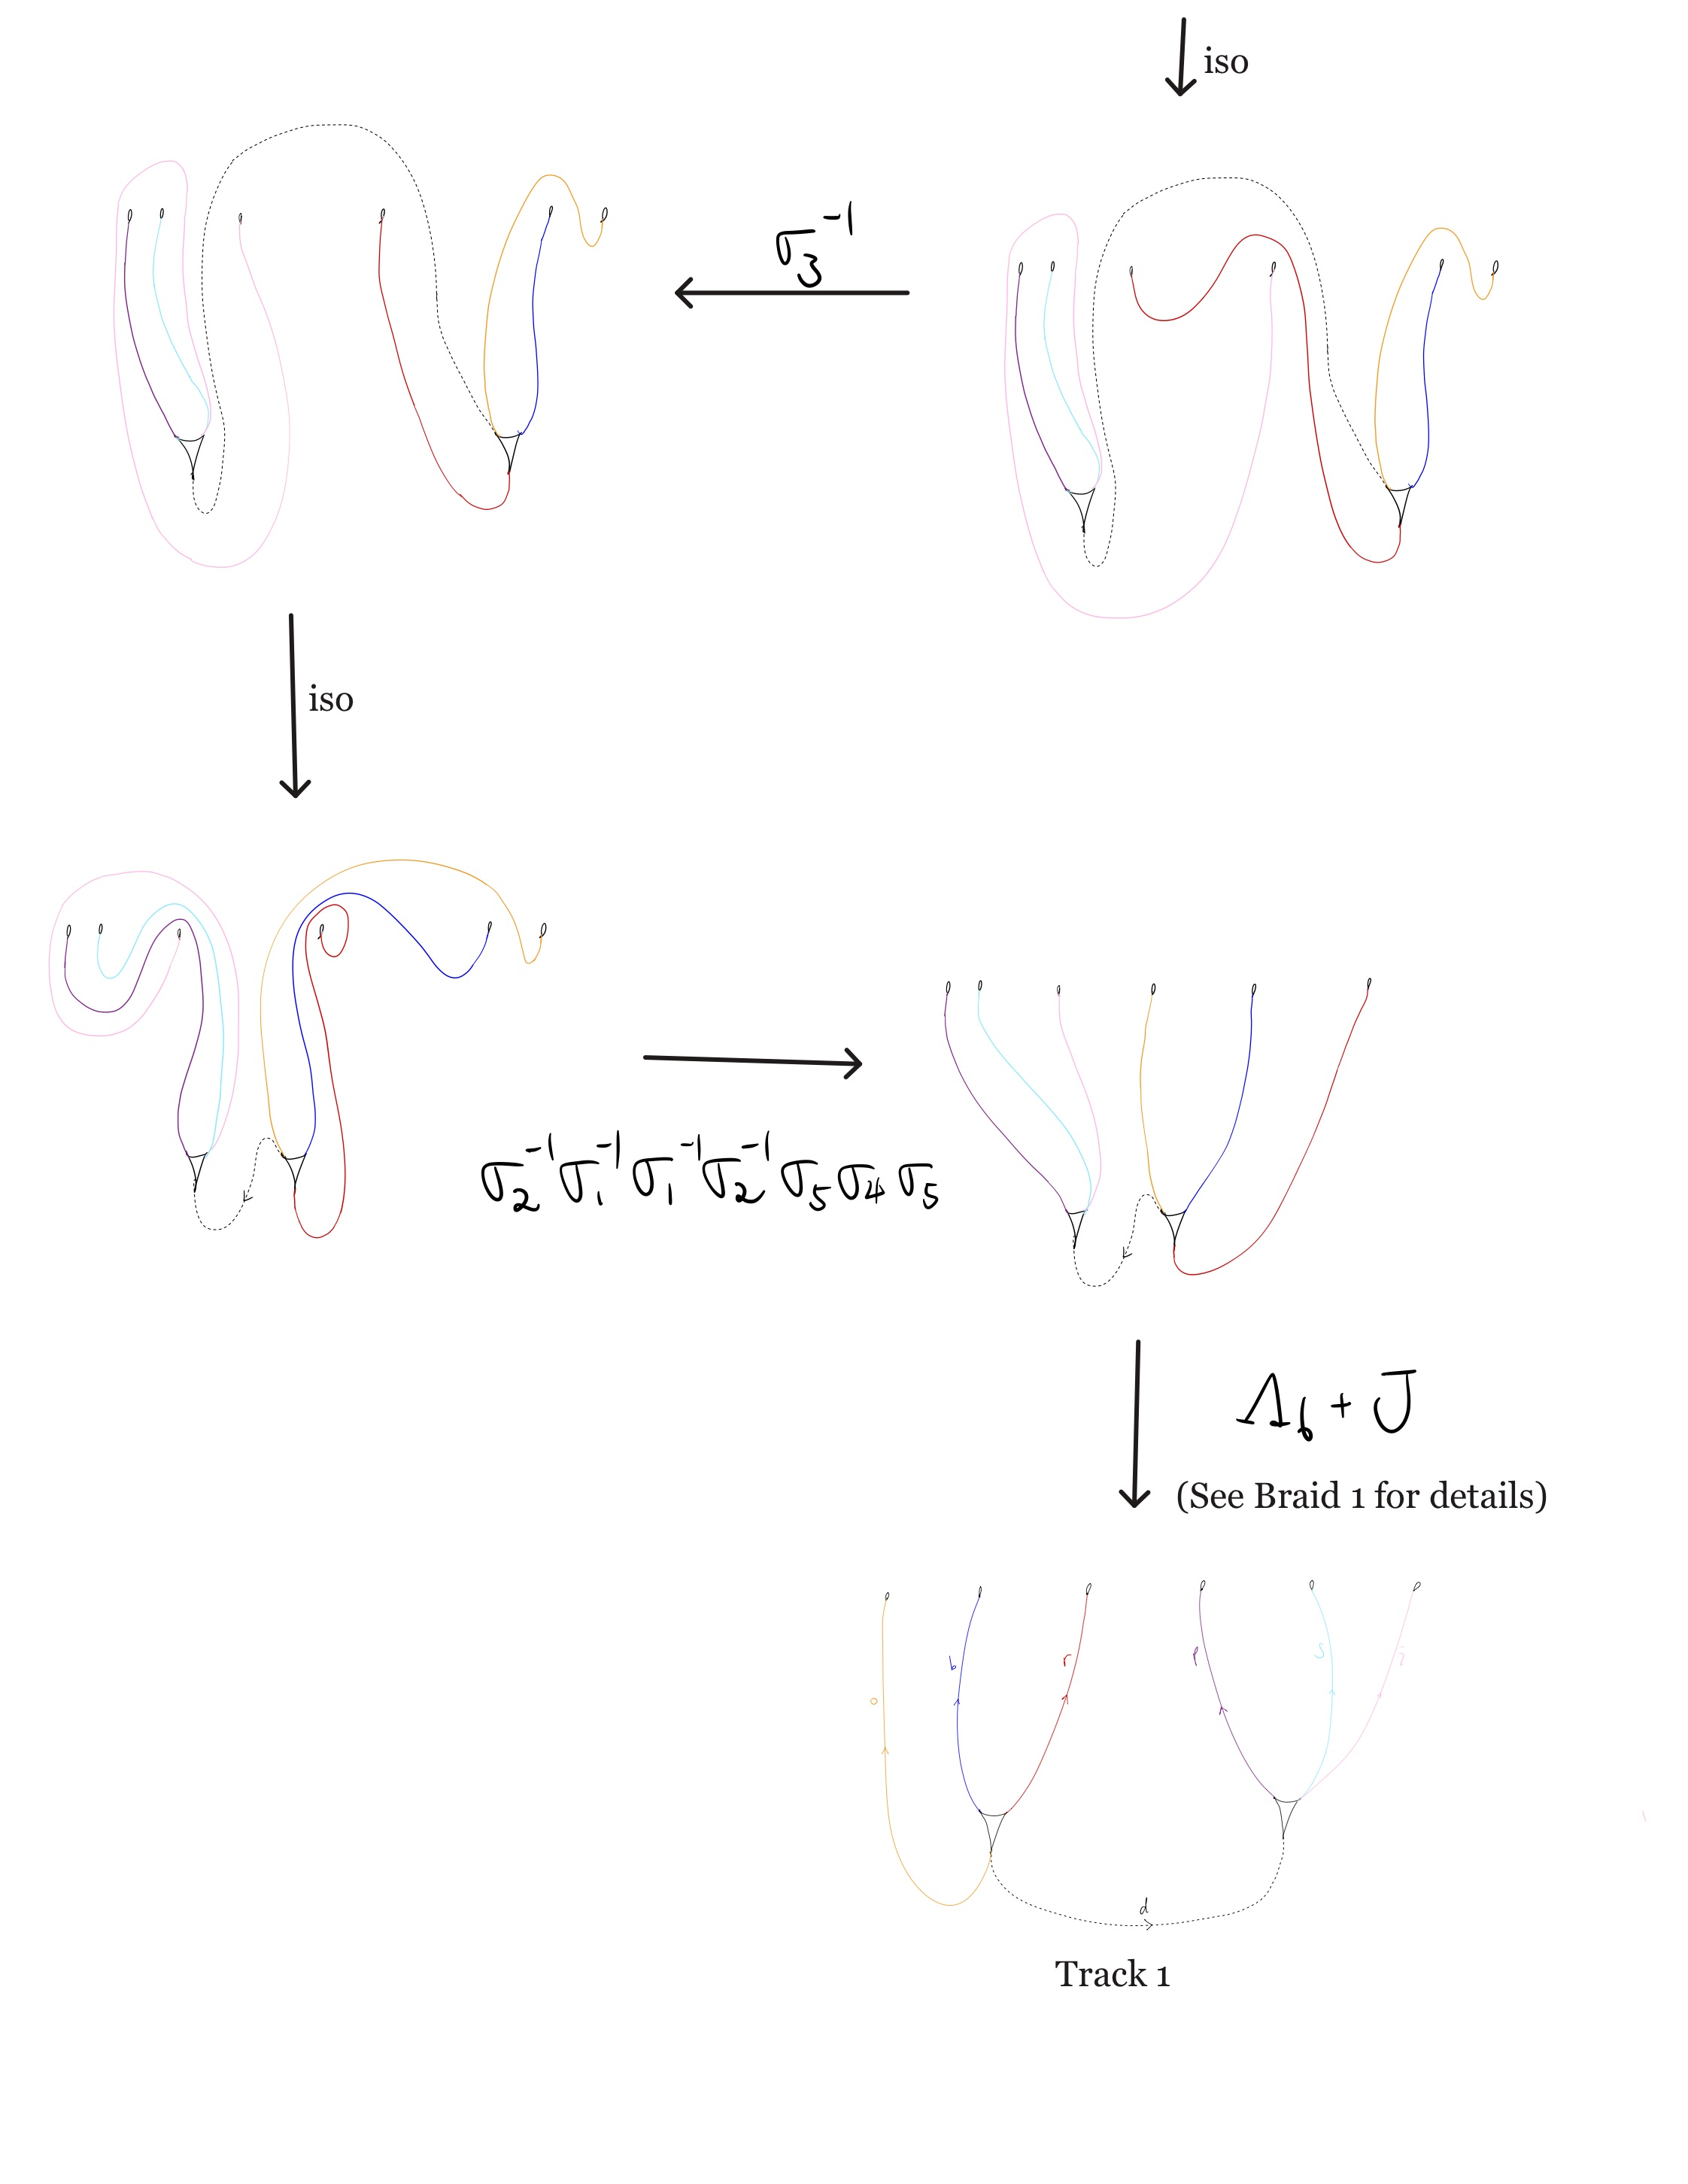
\includegraphics[width=\linewidth, height=0.45\textheight, keepaspectratio]{figures_braid/figures_track_1/Track 1 Braid 11 Dossier-3.jpg}
    \caption{This sequence shows the inverse of the braid $b_{11}^1$ carries Train Track Candidate Family 11.}
    \label{fig:track1_braid_b1_11}
\end{figure*}

\clearpage

\section{Candidate Family 12 (Querulous)}\label{sec:track1_querulous_1}
Train Track Map Candidate Family 12 of Track 1 is shown in Figure \ref{fig:track1_braid_b1_12_map}. See \ref{Querulous} for details.

\begin{figure*}[ht]
    \centering
    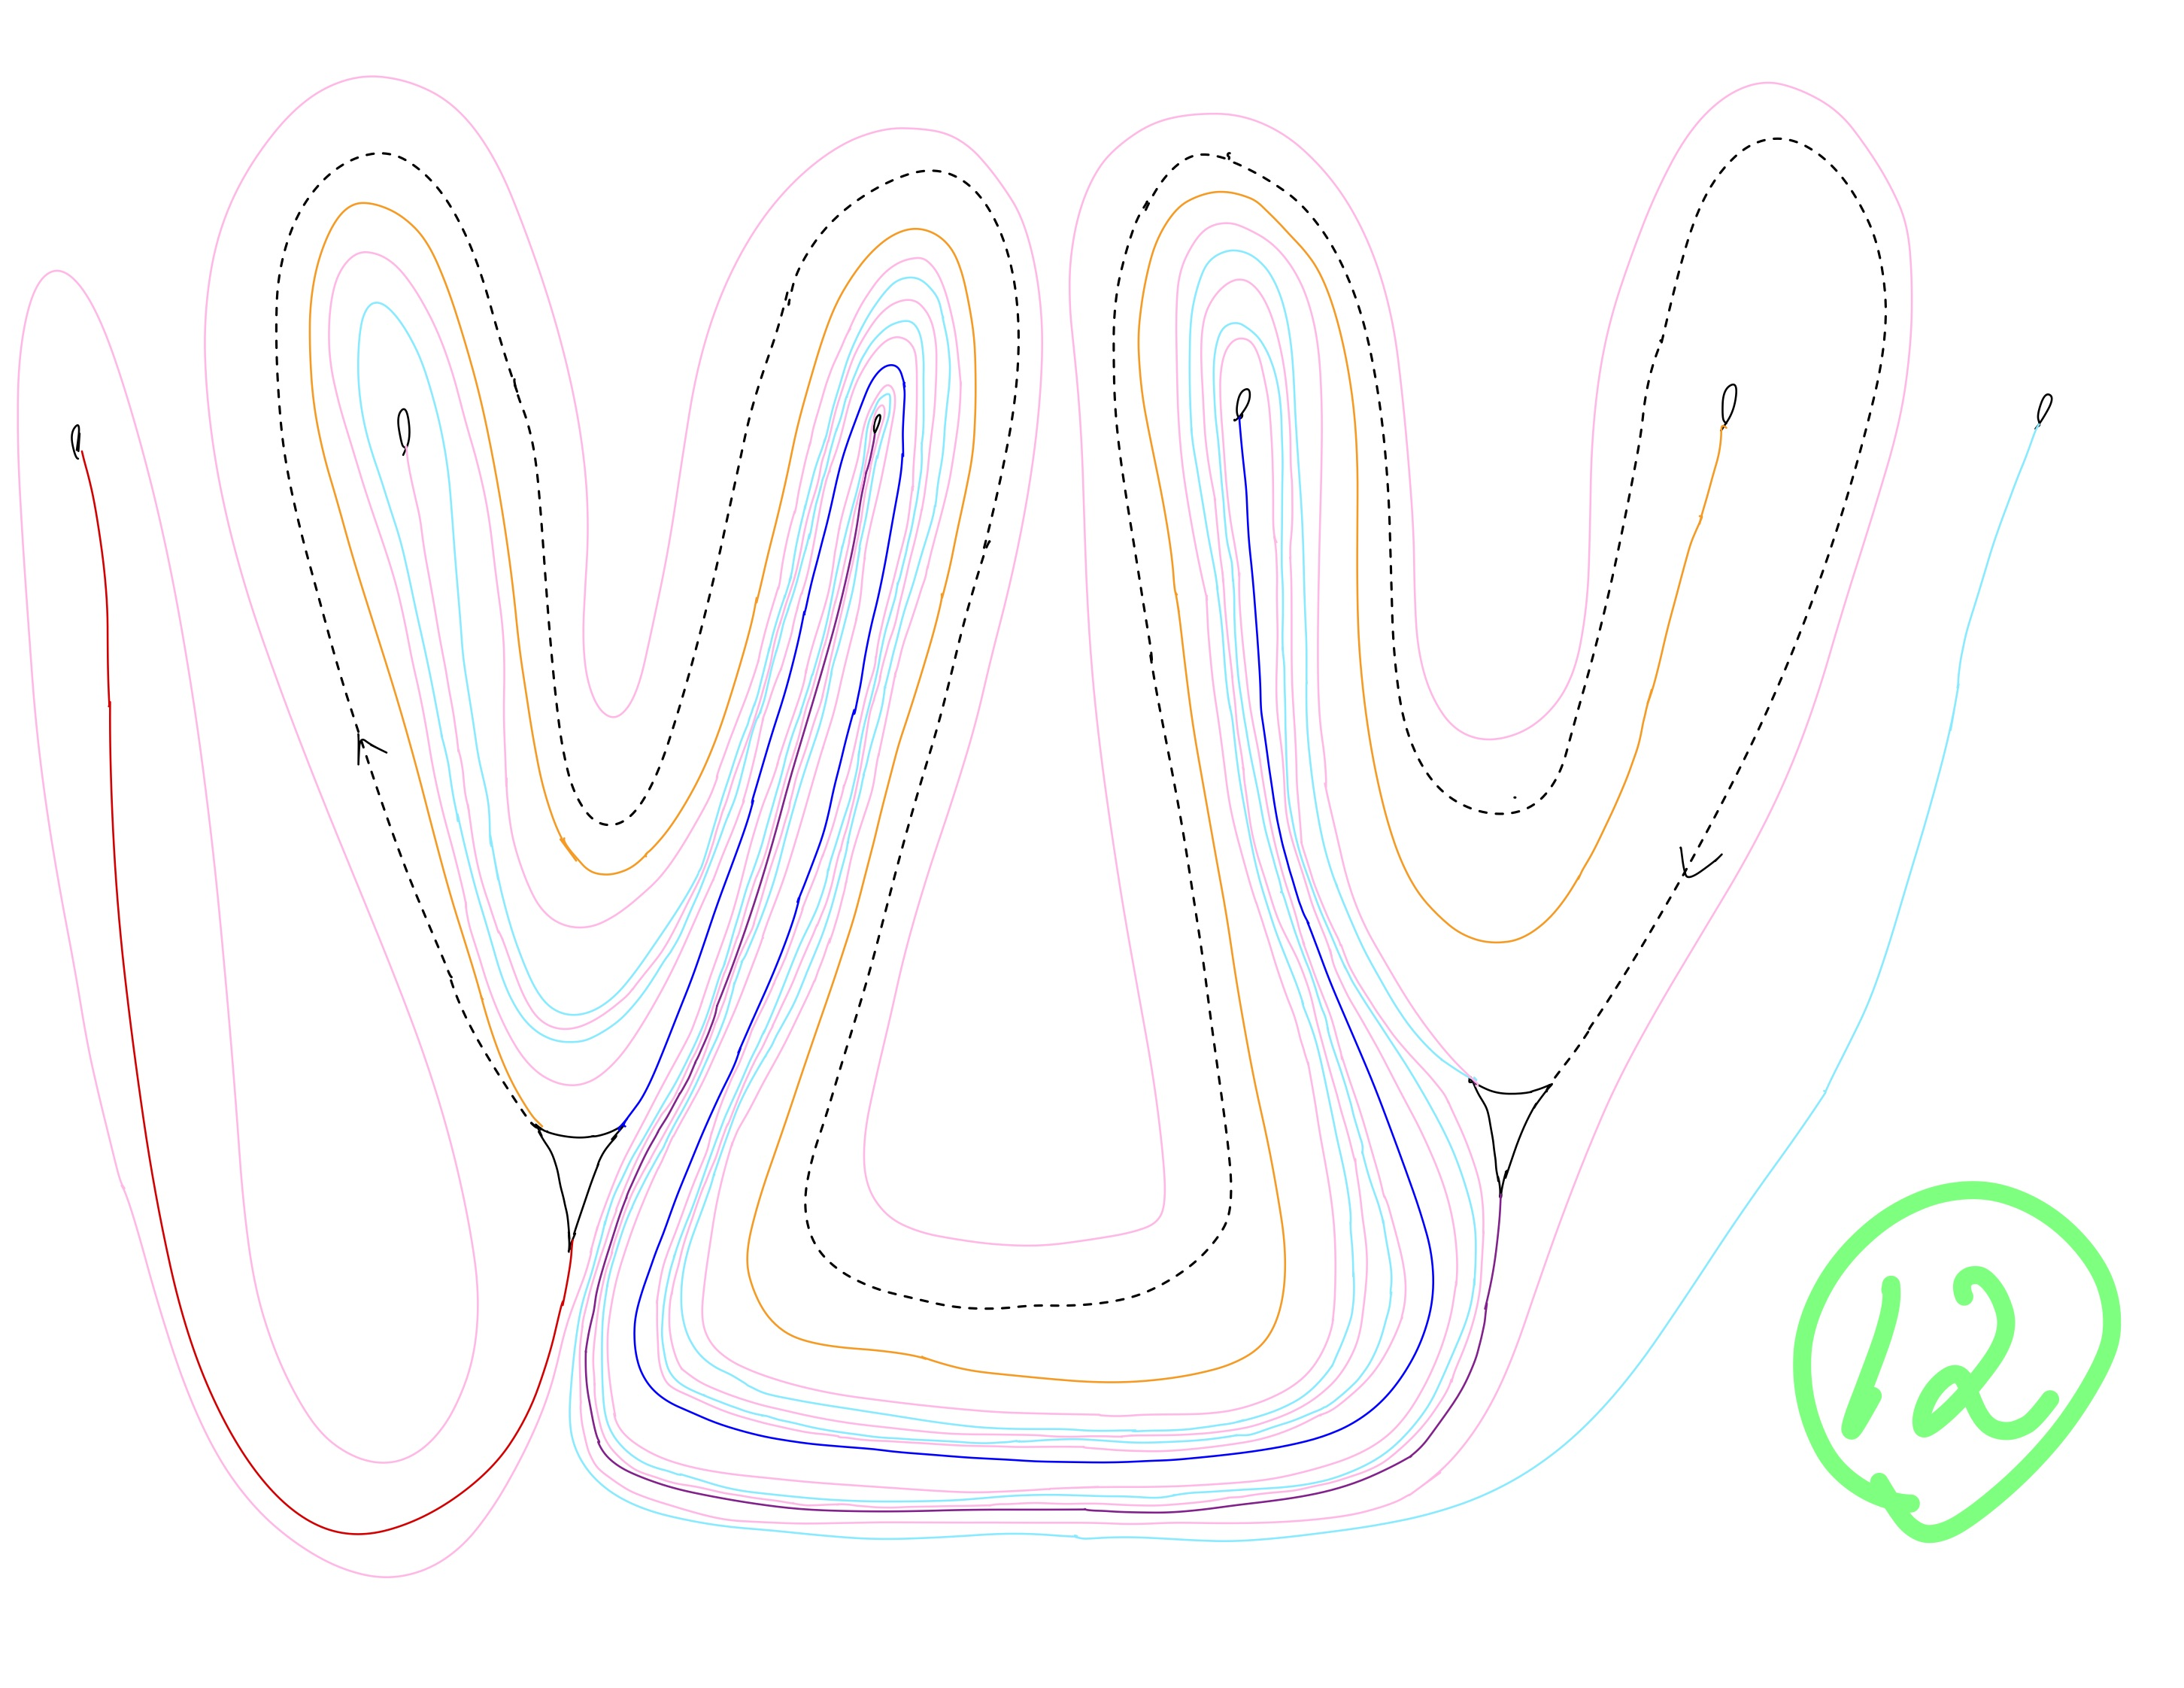
\includegraphics[width=\linewidth, height=0.45\textheight, keepaspectratio]{figures_braid/figures_track_1/Track 1 Braid 12 Querulous-1.jpg}
    \caption{Train Track Map Candidate Family 12 (Querulous) of Track 1.}
    \label{fig:track1_braid_b1_12_map}
\end{figure*}

The inverse of the following braid carries this family of train track maps:
\[
b_{12}^1 = \sigma_{4} \sigma_{3} \sigma_{2} \sigma_{3}^{-1} \sigma_{4}^{-1} \sigma_{3} \sigma_{4} \sigma_{4} \sigma_{4} \sigma_{3} \sigma_{2} \sigma_{1} \sigma_{1} \sigma_{2} \sigma_{3} \sigma_{1}^{-1} \sigma_{2}^{-1} \sigma_{1}^{-1} \sigma_{1}^{-1} \sigma_{4} \sigma_{5}
\]

This is shown in Figure \ref{fig:track1_braid_b1_12}.

\begin{figure*}[p]
    \centering
    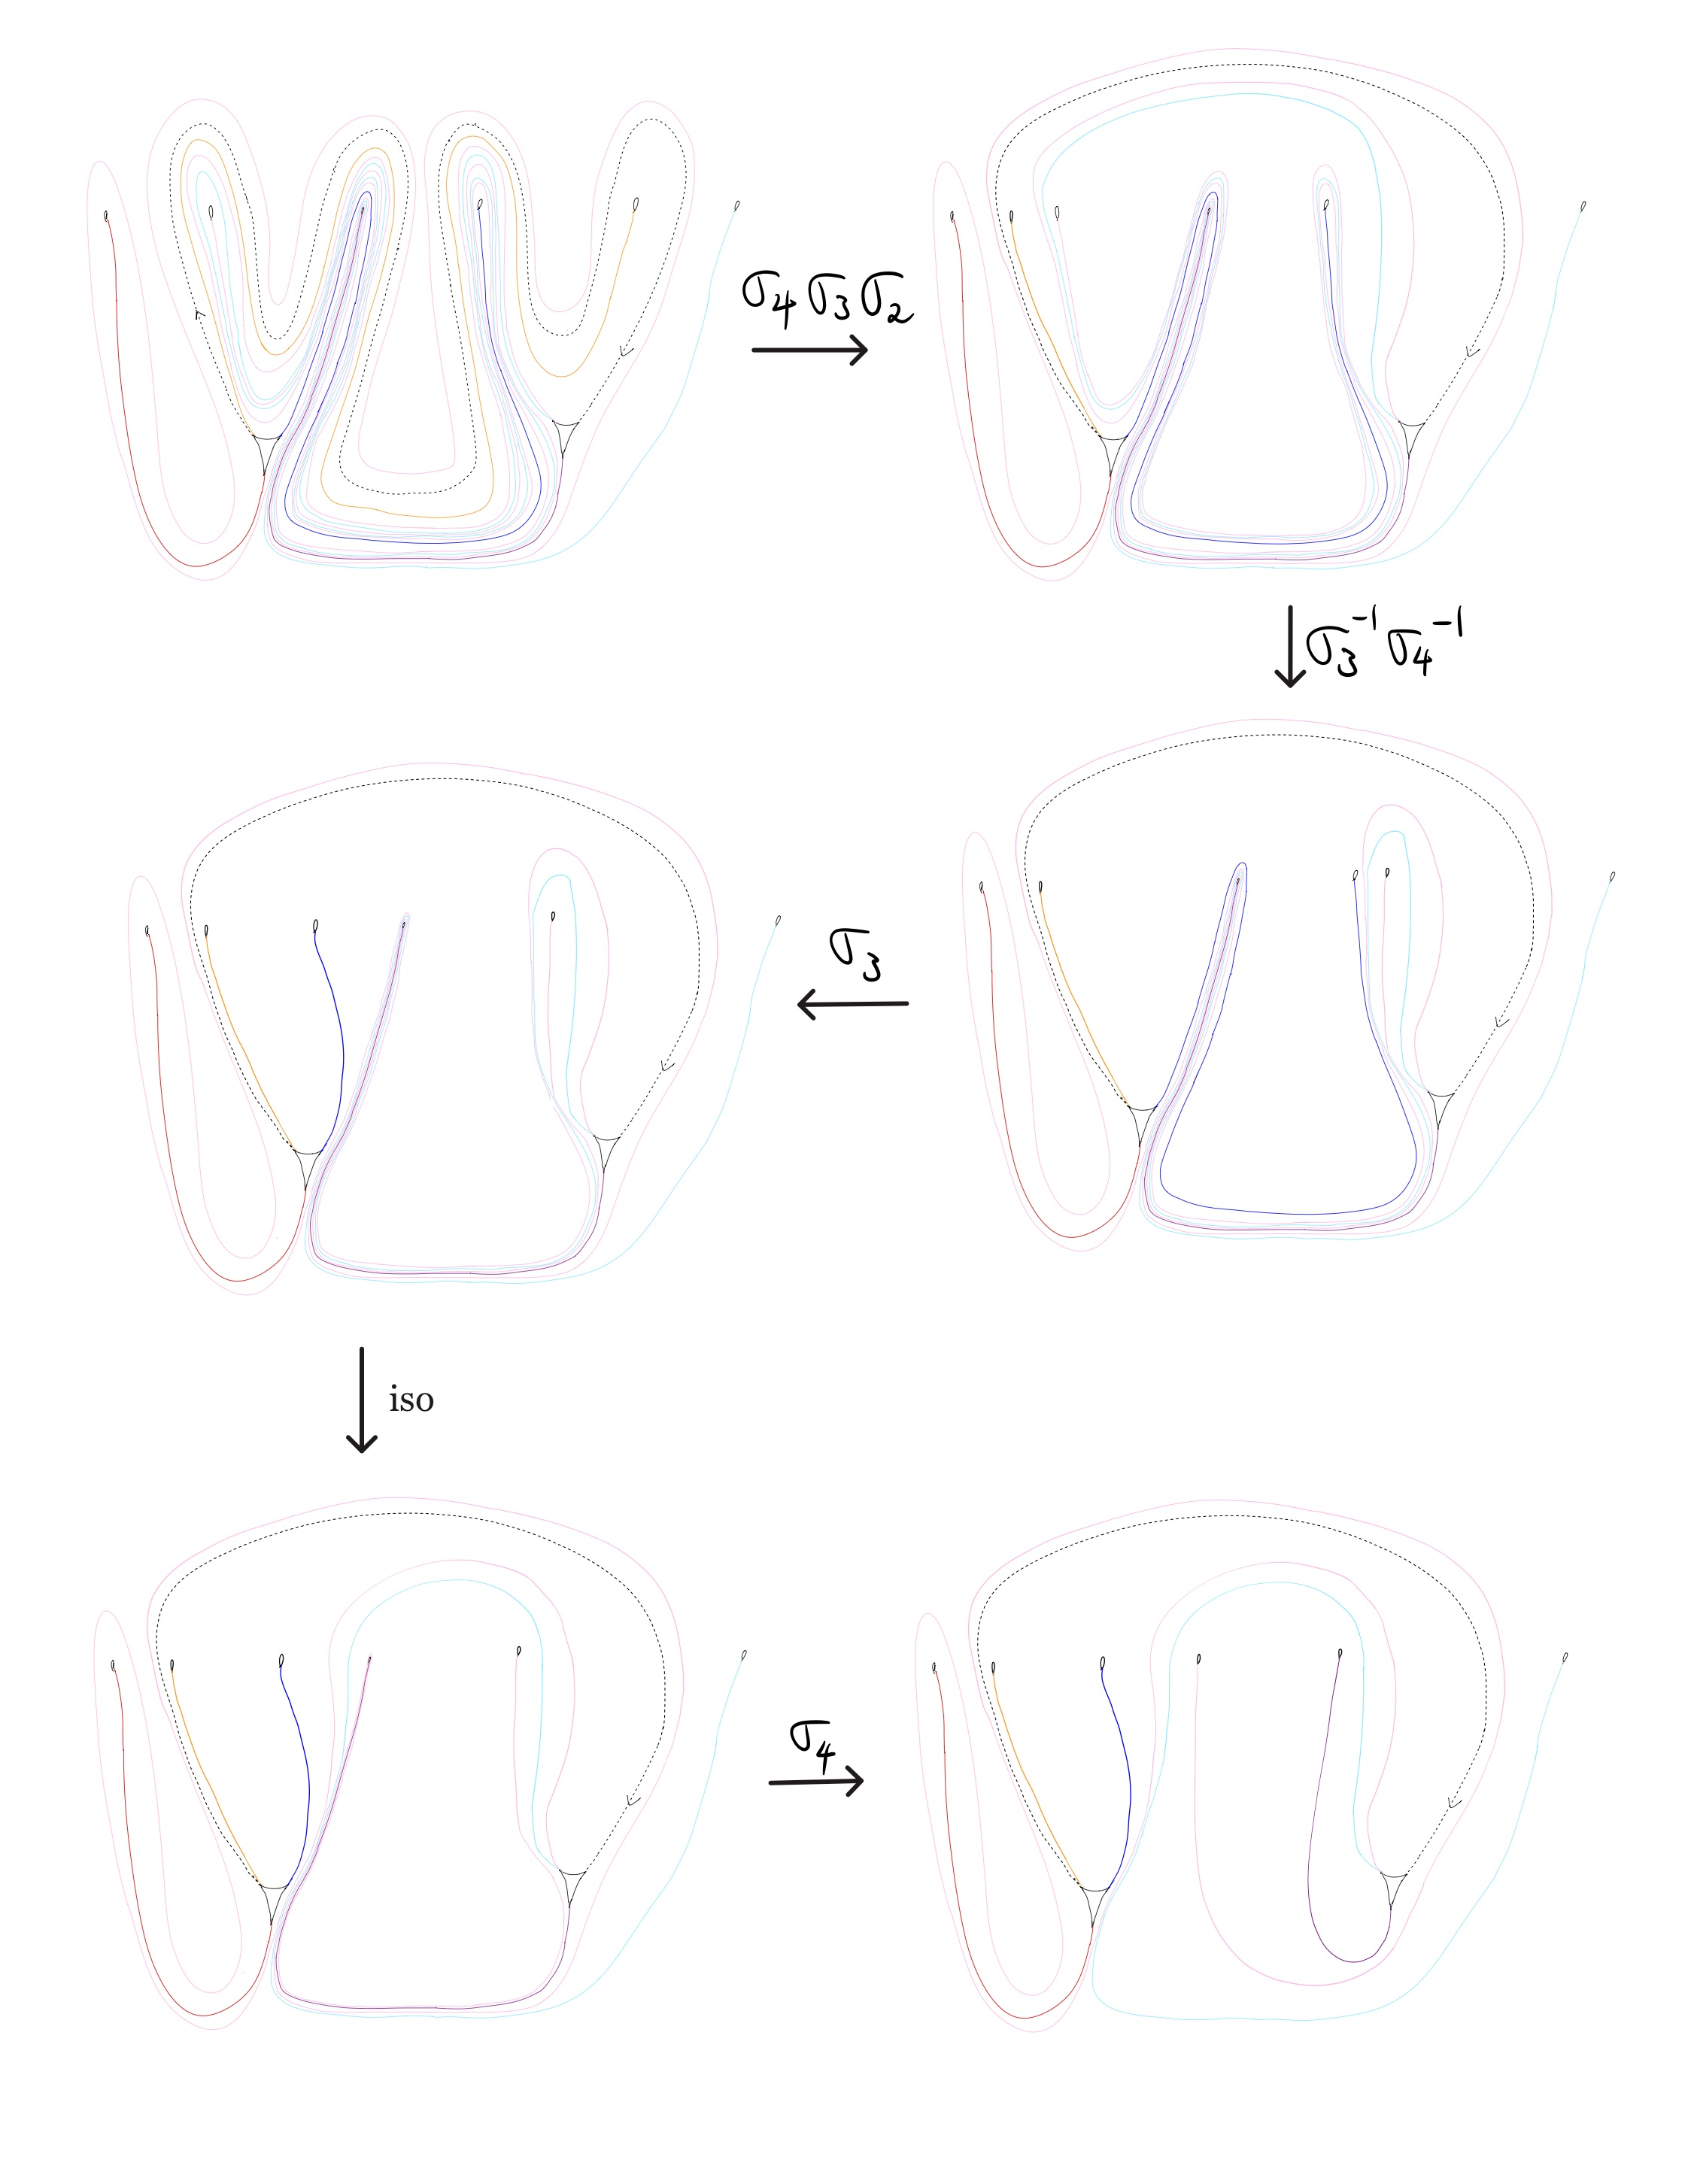
\includegraphics[width=\linewidth, height=0.45\textheight, keepaspectratio]{figures_braid/figures_track_1/Track 1 Braid 12 Querulous-2.jpg}\\
    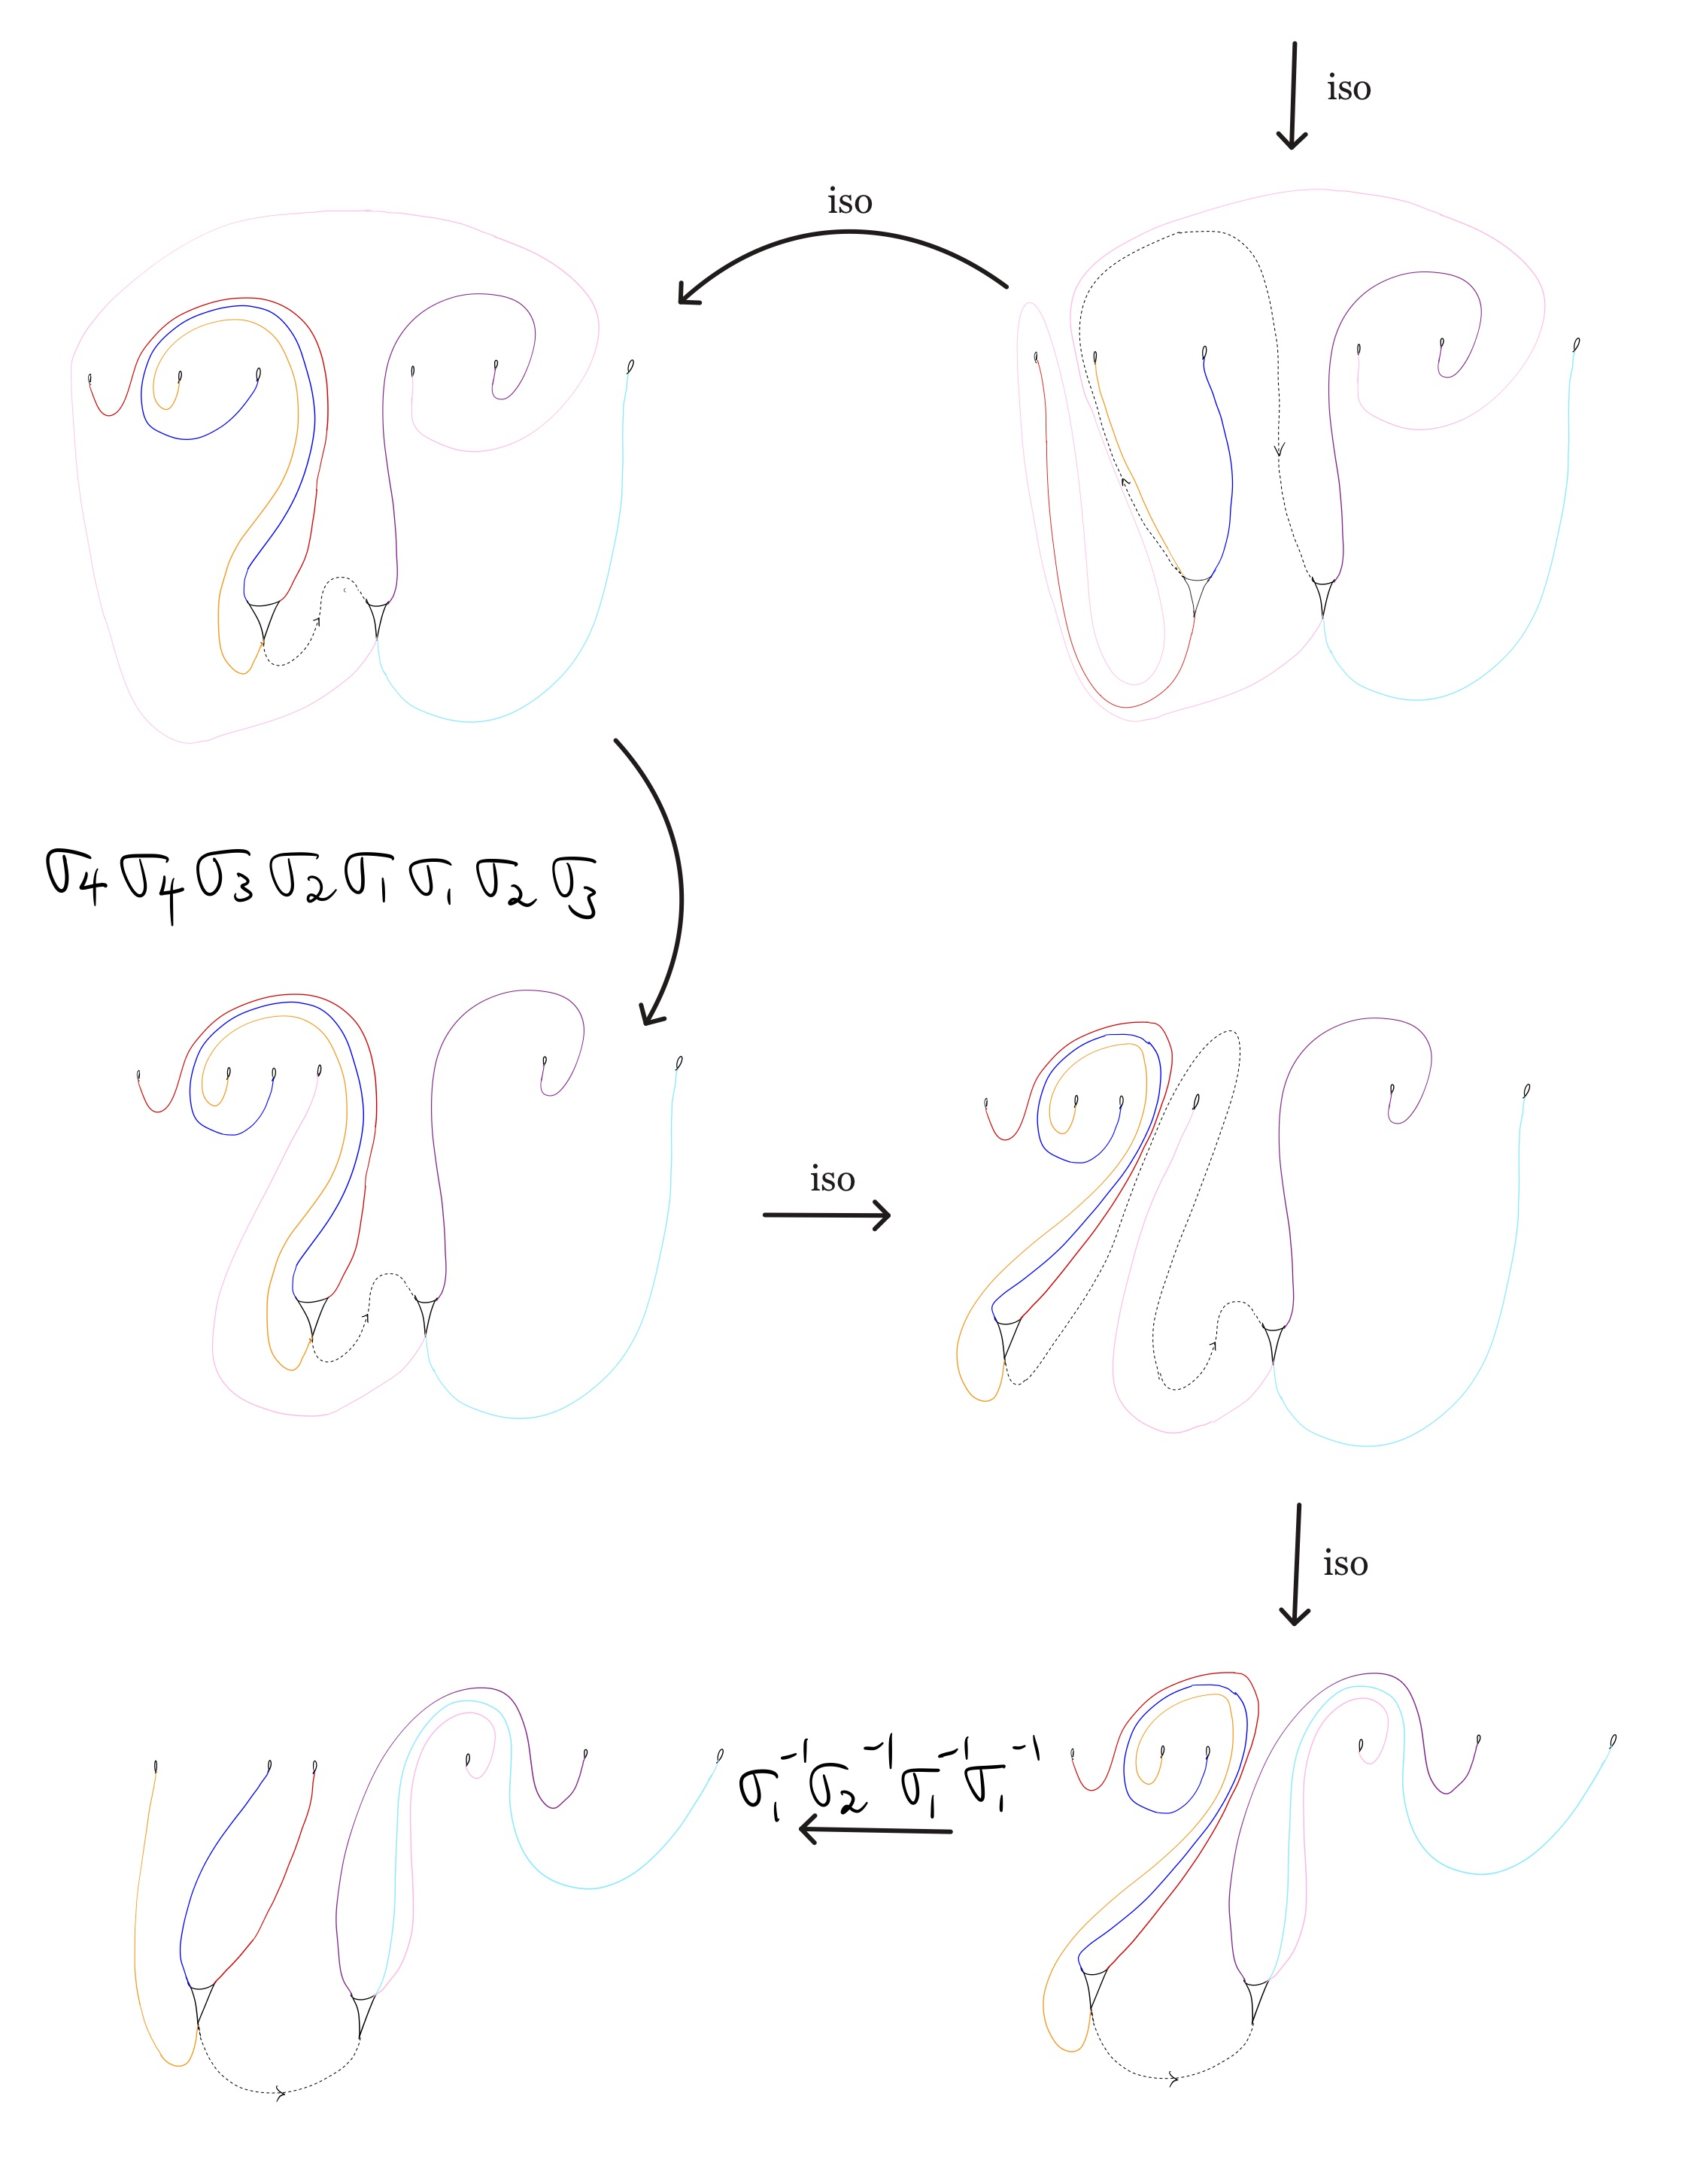
\includegraphics[width=\linewidth, height=0.45\textheight, keepaspectratio]{figures_braid/figures_track_1/Track 1 Braid 12 Querulous-3.jpg}
    \caption{This sequence shows the inverse of the braid $b_{12}^1$ carries Train Track Candidate Family 12.}
    \label{fig:track1_braid_b1_12}
\end{figure*}

\clearpage

\section{Candidate Family 13 (Querulous)}\label{sec:track1_querulous_2}
Train Track Map Candidate Family 13 of Track 1 is shown in Figure \ref{fig:track1_braid_b1_13_map}. See \ref{Querulous} for details.

\begin{figure*}[ht]
    \centering
    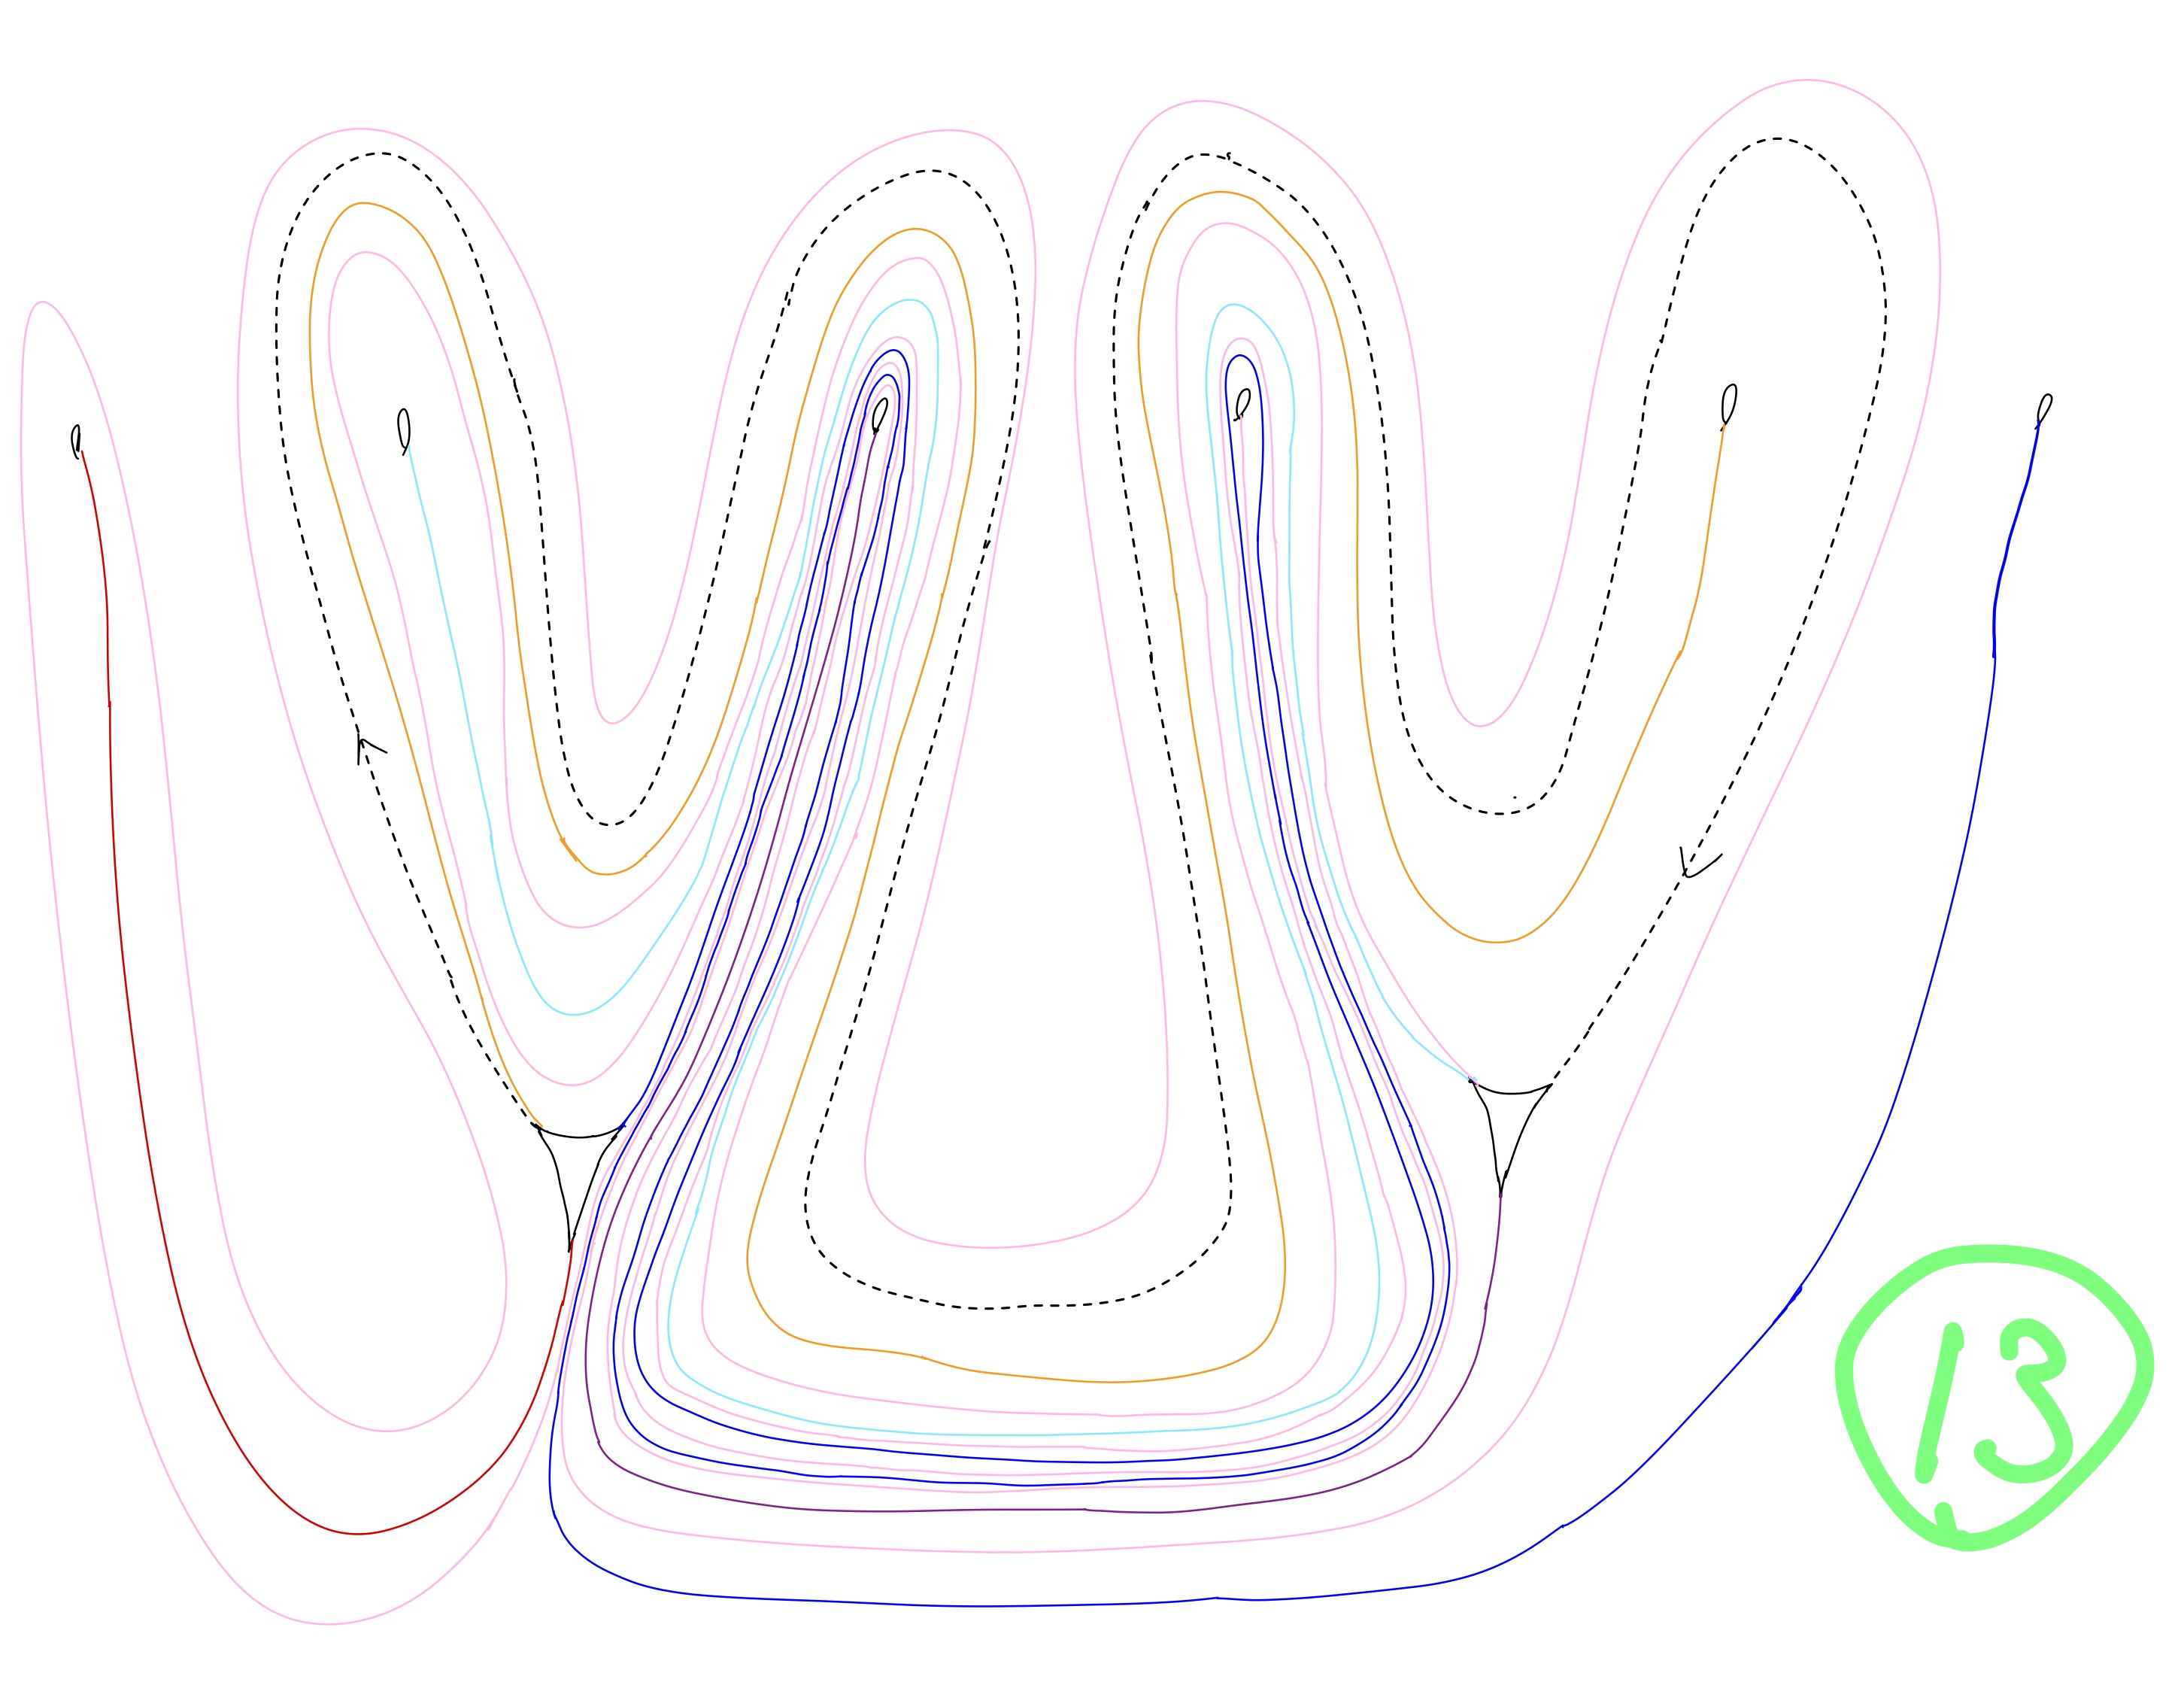
\includegraphics[width=\linewidth, height=0.45\textheight, keepaspectratio]{figures_braid/figures_track_1/Track 1 Braid 13 Querulous-1.jpg}
    \caption{Train Track Map Candidate Family 13 (Querulous) of Track 1.}
    \label{fig:track1_braid_b1_13_map}
\end{figure*}

The inverse of the following braid carries this family of train track maps:
\[
b_{13}^1 = \sigma_{4} \sigma_{3} \sigma_{2} \sigma_{3}^{-1} \sigma_{4}^{-1} \sigma_{3} \sigma_{2}^{-1} \sigma_{1}^{-1} \sigma_{1}^{-1} \sigma_{2}^{-1} \sigma_{3}^{-1} \sigma_{4}^{-1} \sigma_{3} \sigma_{4}^{-1} \sigma_{5}^{-1} \sigma_{3}^{-1} \sigma_{4}^{-1} \sigma_{3}^{-1} \sigma_{1}^{-1} \sigma_{2}^{-1} \sigma_{1}^{-1} \sigma_{1}^{-1} \sigma_{5} \sigma_{4} \sigma_{5}
\]

This is shown in Figure \ref{fig:track1_braid_b1_13}.

\begin{figure*}[p]
    \centering
    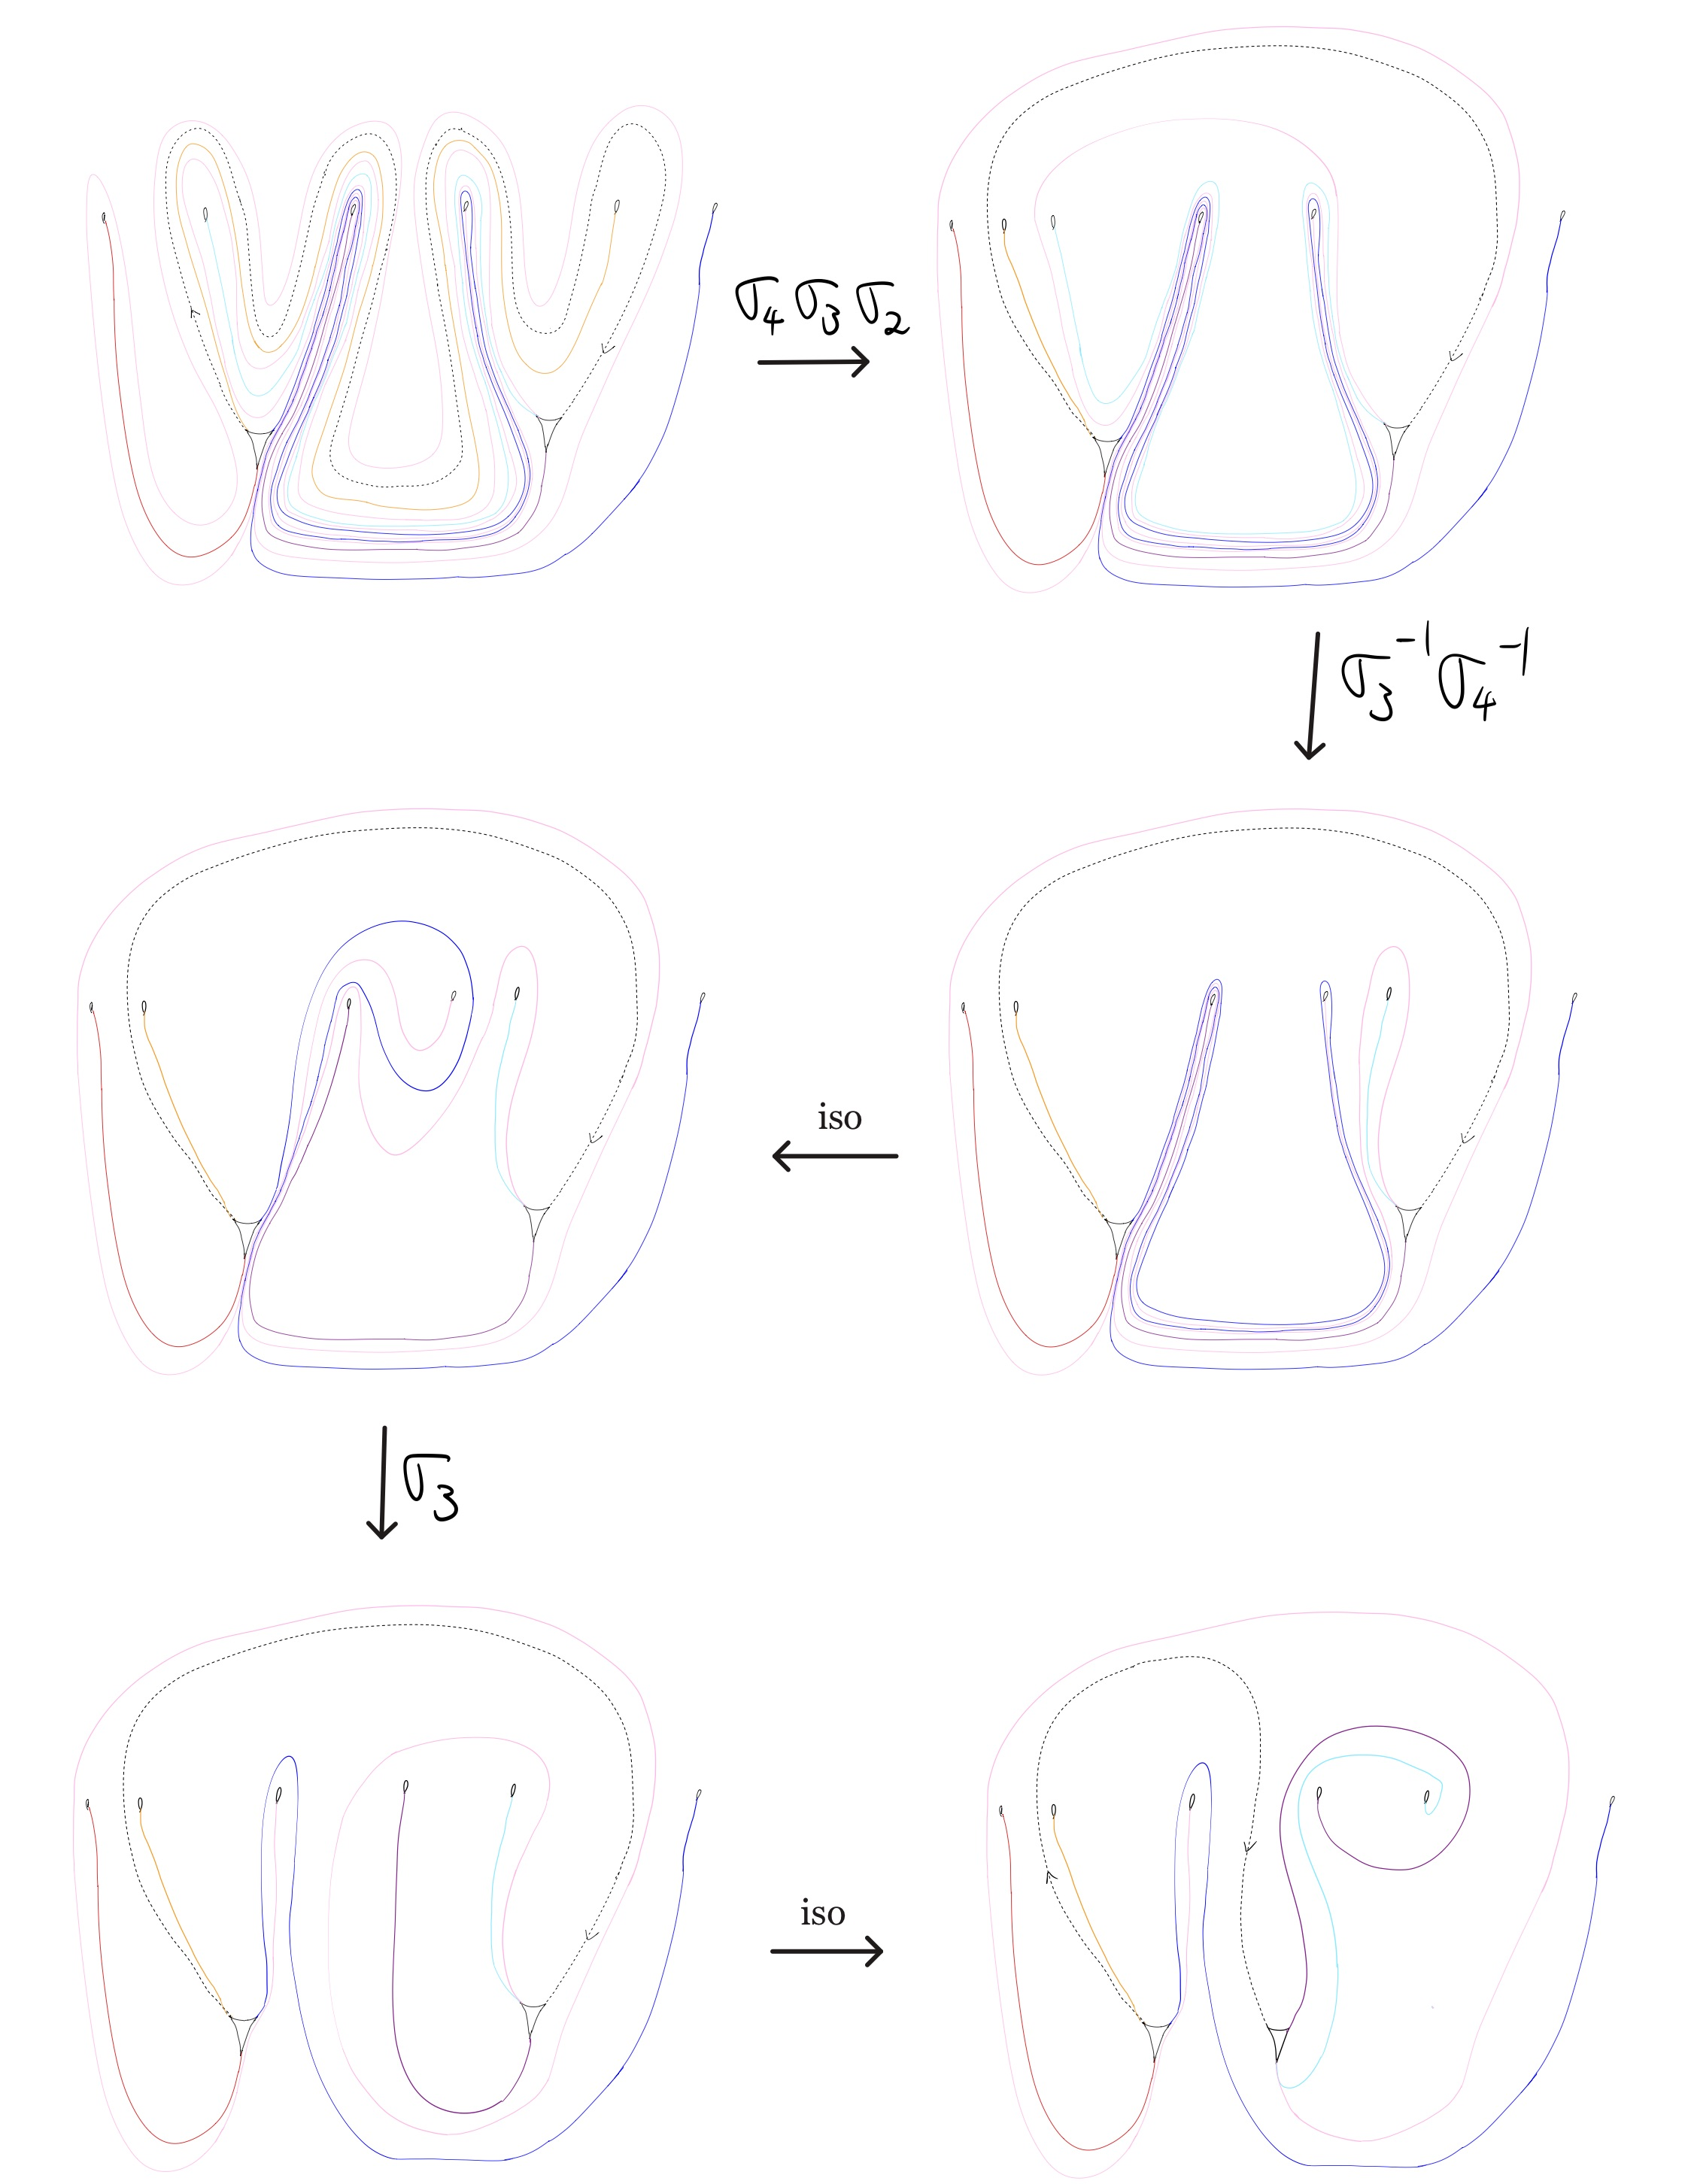
\includegraphics[width=\linewidth, height=0.45\textheight, keepaspectratio]{figures_braid/figures_track_1/Track 1 Braid 13 Querulous-2.jpg}\\
    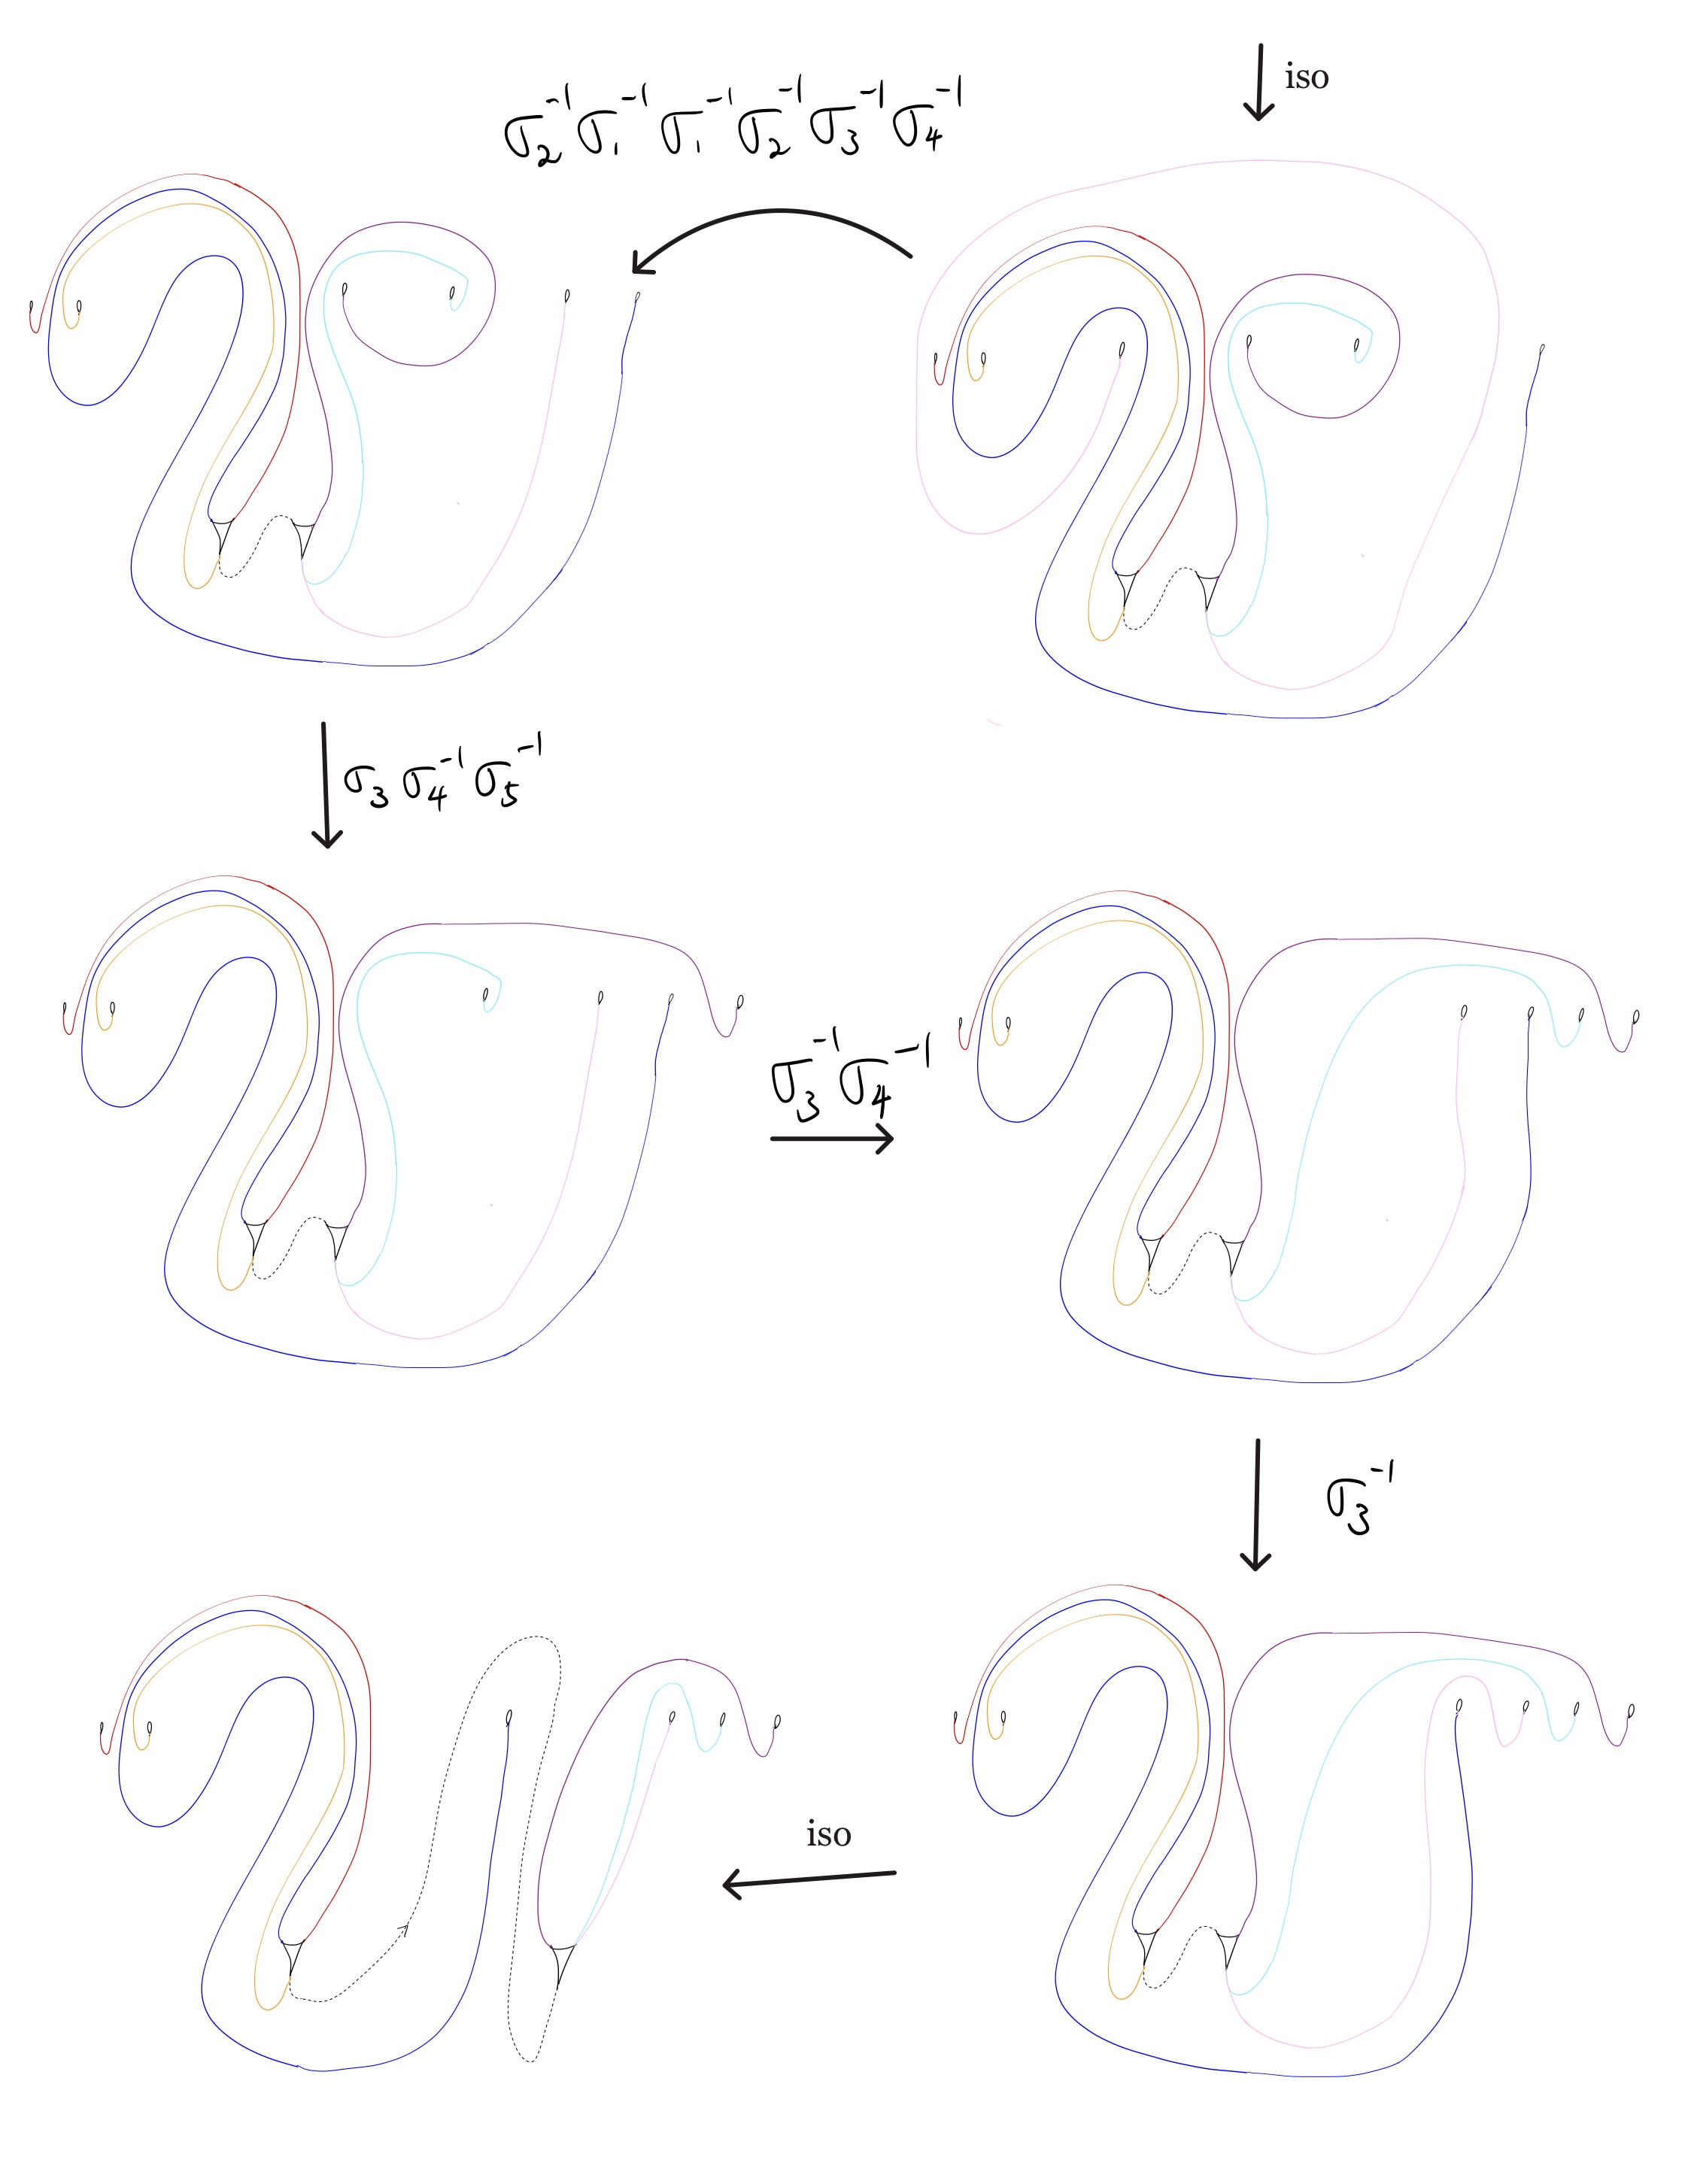
\includegraphics[width=\linewidth, height=0.45\textheight, keepaspectratio]{figures_braid/figures_track_1/Track 1 Braid 13 Querulous-3.jpg}
    \caption{This sequence shows the inverse of the braid $b_{13}^1$ carries Train Track Candidate Family 13.}
    \label{fig:track1_braid_b1_13}
\end{figure*}

\clearpage

\section{Candidate Family 14 (Sybaritic)}\label{sec:track1_sybaritic}
Train Track Map Candidate Family 14 of Track 1 is shown in Figure \ref{fig:track1_braid_b1_14_map}. See \ref{Sybaritic} for details.

\begin{figure*}[ht]
    \centering
    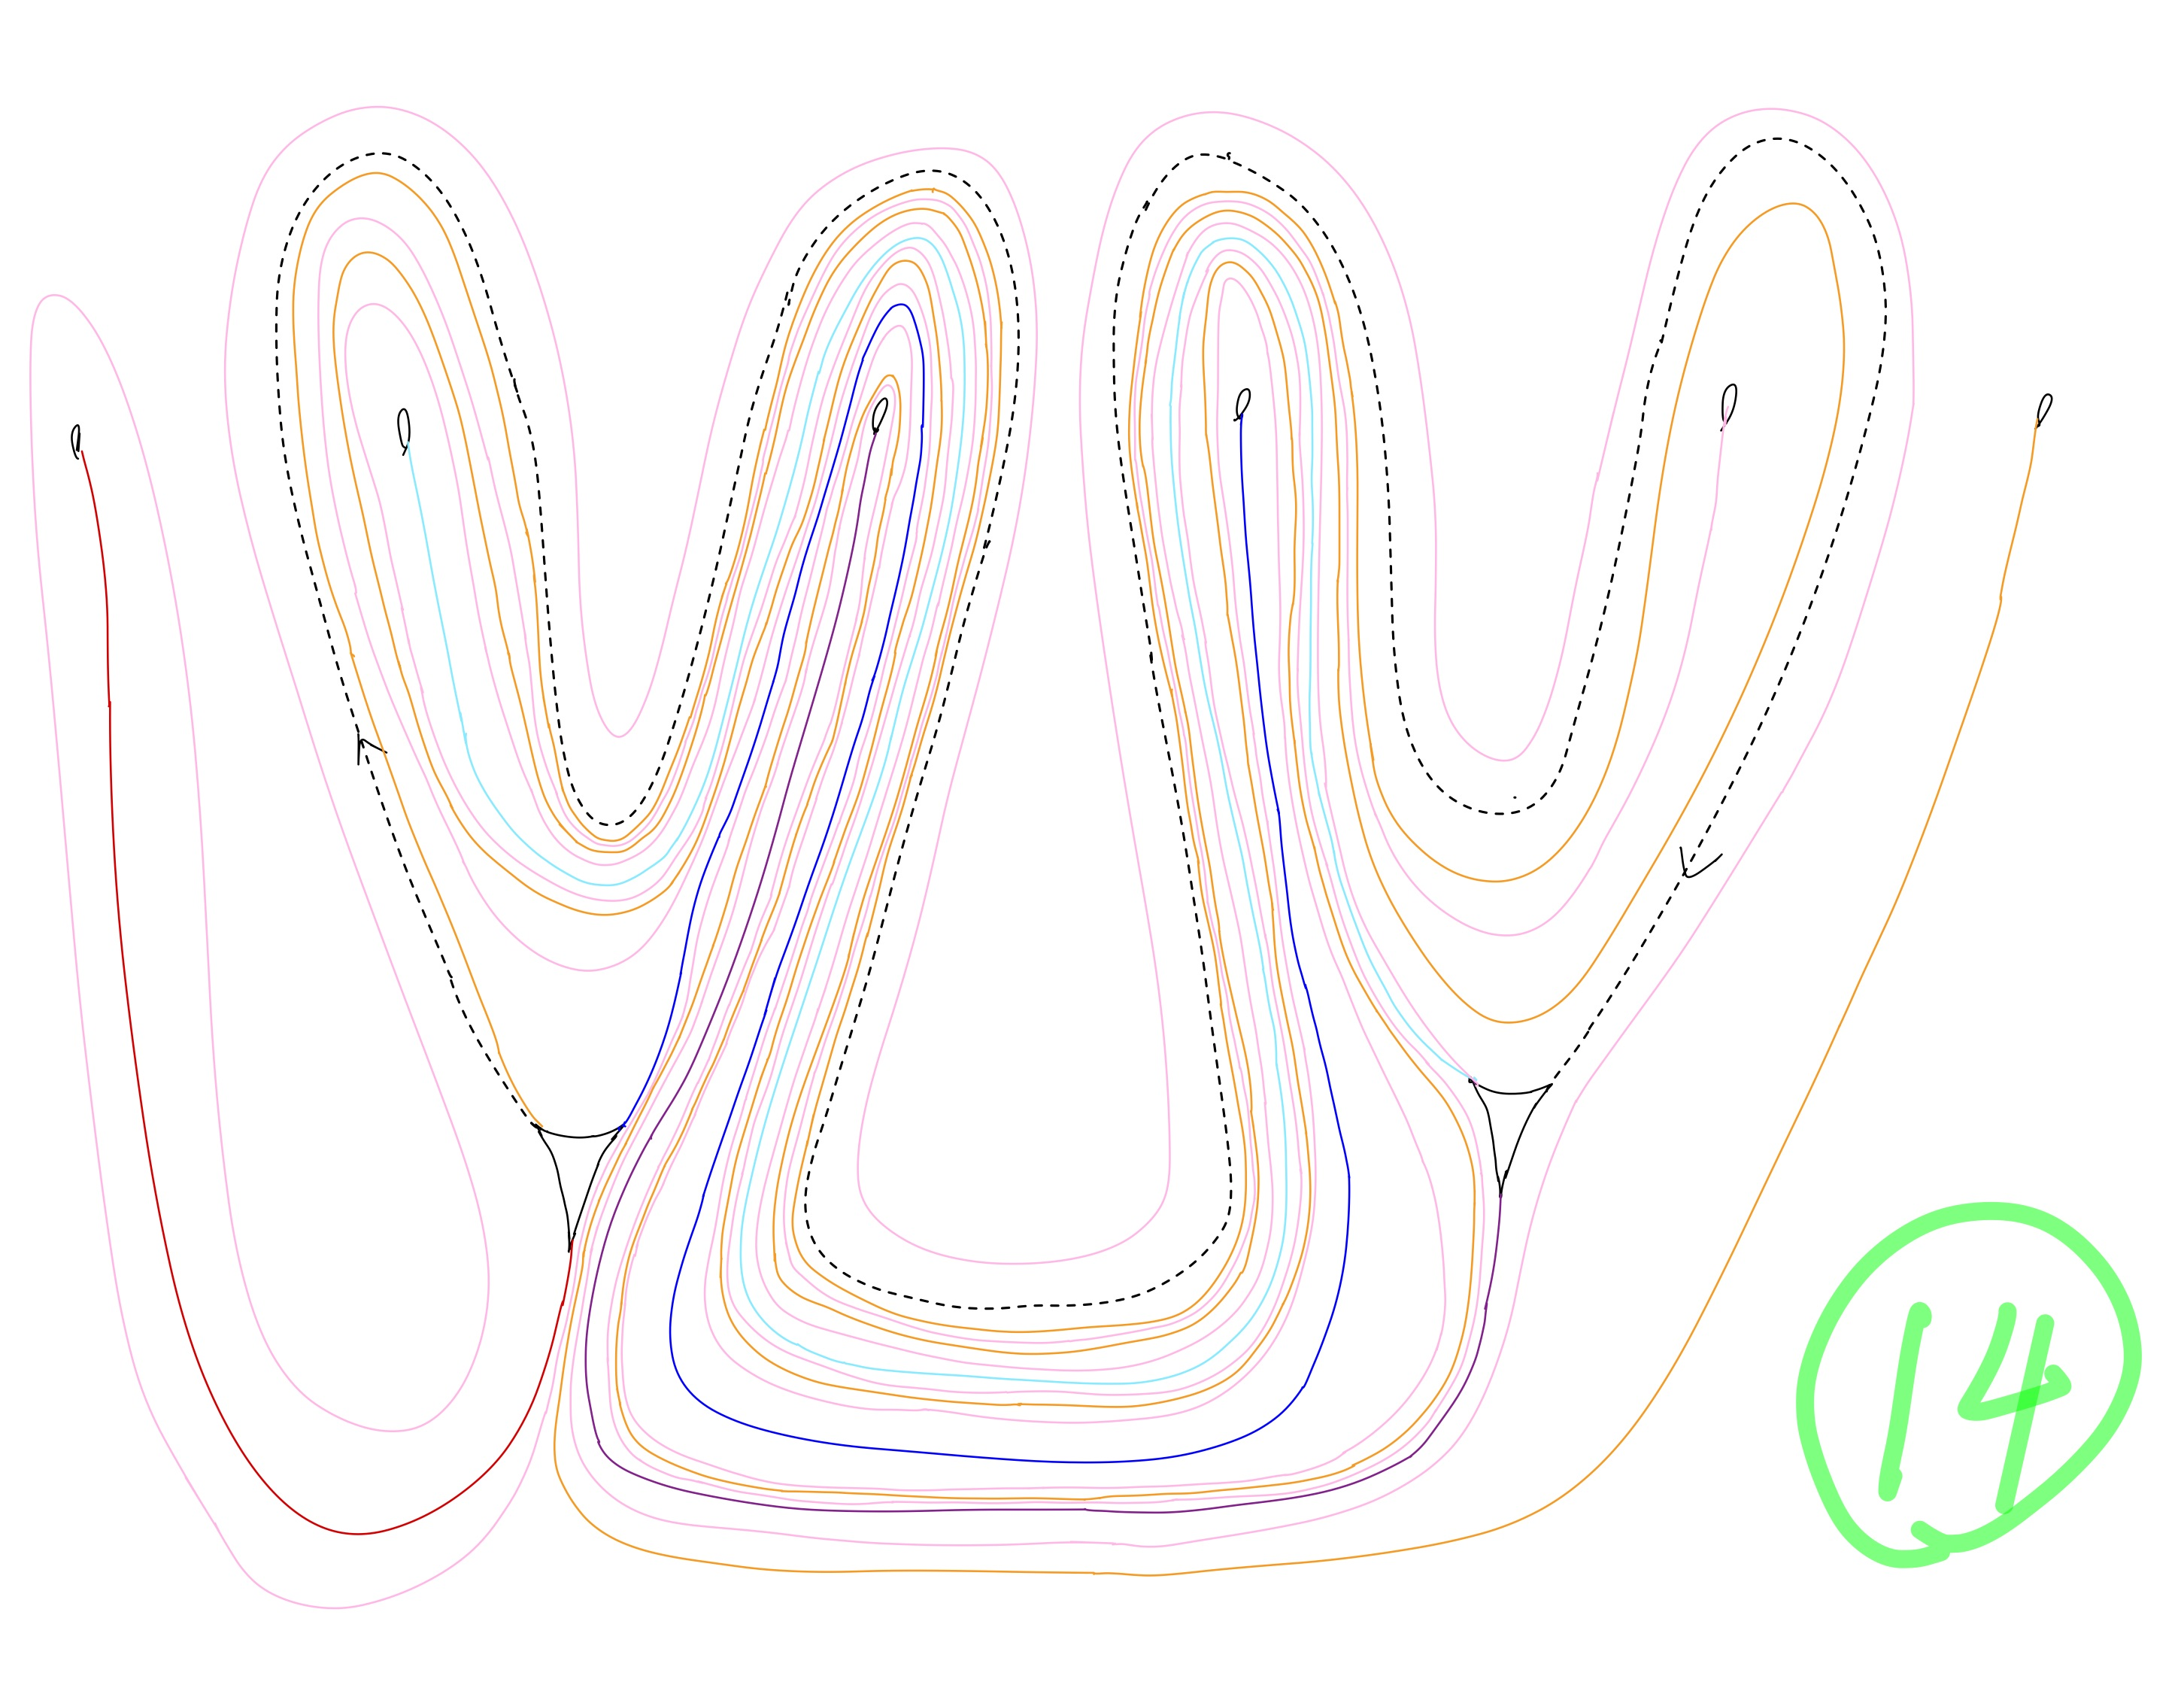
\includegraphics[width=\linewidth, height=0.45\textheight, keepaspectratio]{figures_braid/figures_track_1/Track 1 Braid 14 Sybaritic-1.jpg}
    \caption{Train Track Map Candidate Family 14 (Sybaritic) of Track 1.}
    \label{fig:track1_braid_b1_14_map}
\end{figure*}

The inverse of the following braid carries this family of train track maps:
\[
b_{14}^1 = \sigma_{4} \sigma_{3} \sigma_{2} \sigma_{3}^{-1} \sigma_{4}^{-1} \sigma_{2}^{-1} \sigma_{3}^{-1} \sigma_{2} \sigma_{3} \sigma_{2}^{-1} \sigma_{1}^{-1} \sigma_{1}^{-1} \sigma_{2}^{-1} \sigma_{3}^{-1} \sigma_{4}^{-1} \sigma_{5}^{-1} \sigma_{3} \sigma_{4}^{-1} \sigma_{5}^{-1} \sigma_{3}^{-1} \sigma_{4}^{-1} \sigma_{1}^{-1} \sigma_{2} \sigma_{1}^{-1} \sigma_{5} \sigma_{4} \sigma_{5}
\]

This is shown in Figure \ref{fig:track1_braid_b1_14}.

\begin{figure*}[p]
    \centering
    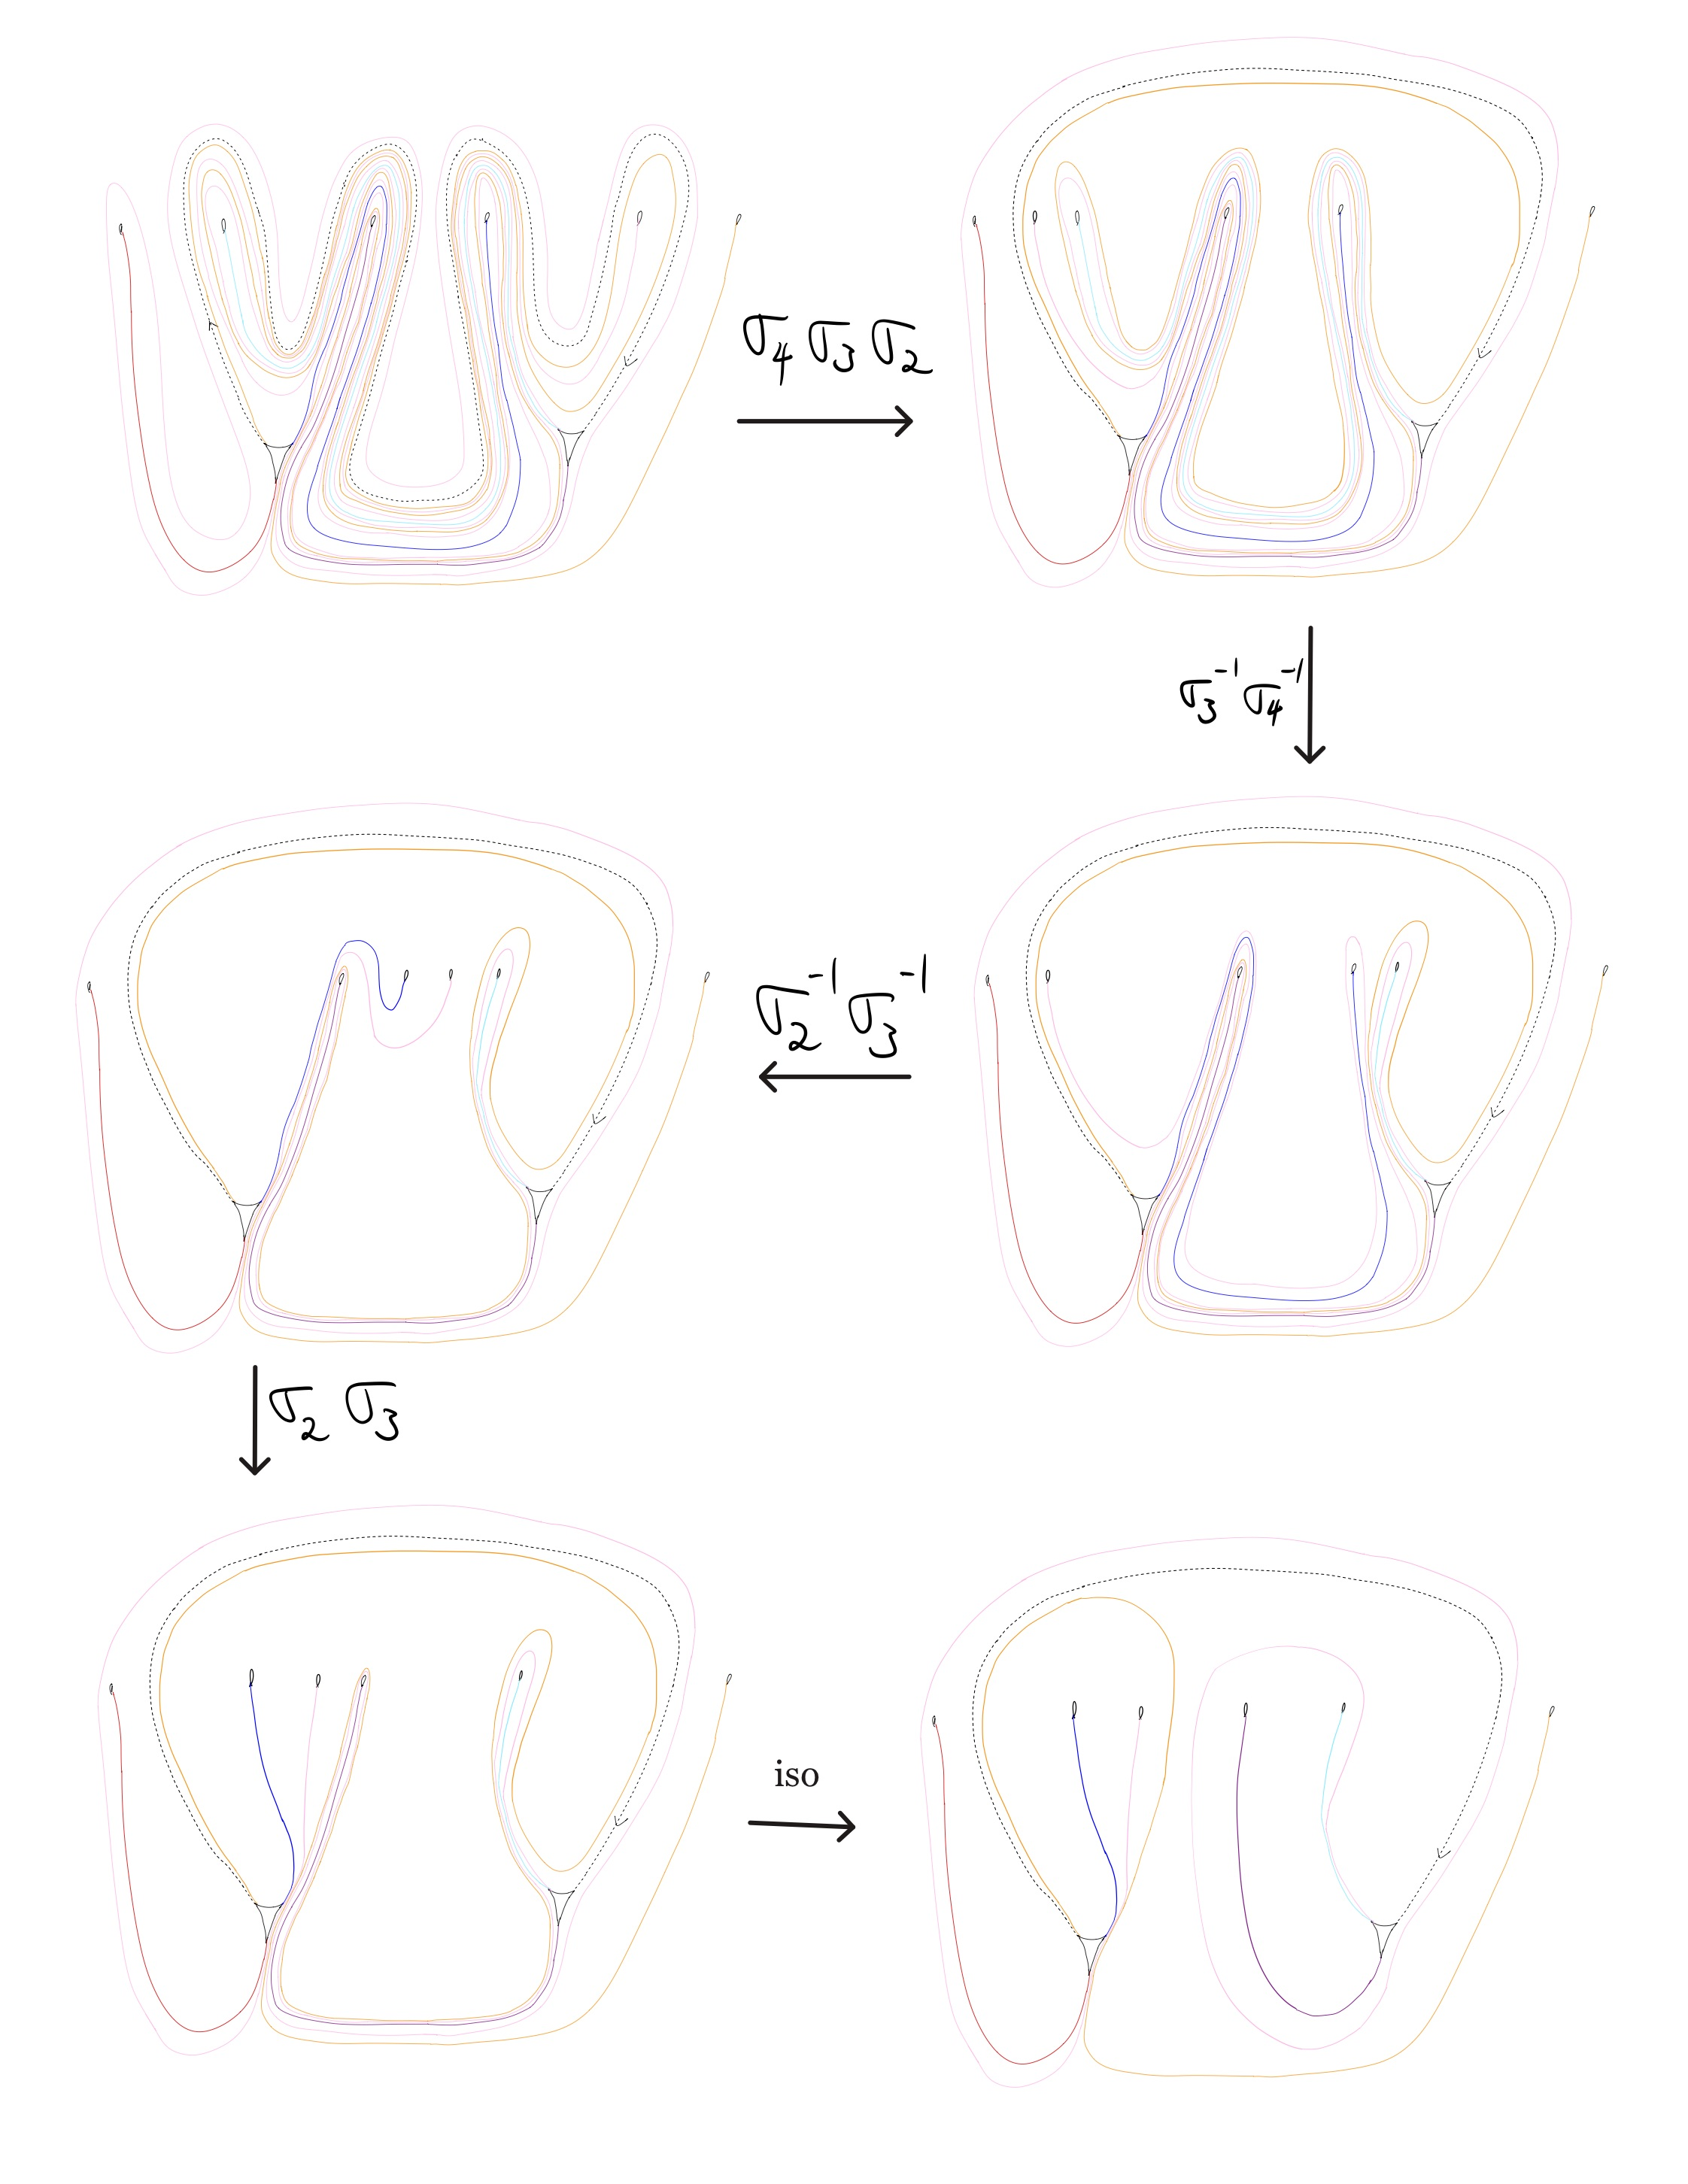
\includegraphics[width=\linewidth, height=0.45\textheight, keepaspectratio]{figures_braid/figures_track_1/Track 1 Braid 14 Sybaritic-2.jpg}\\
    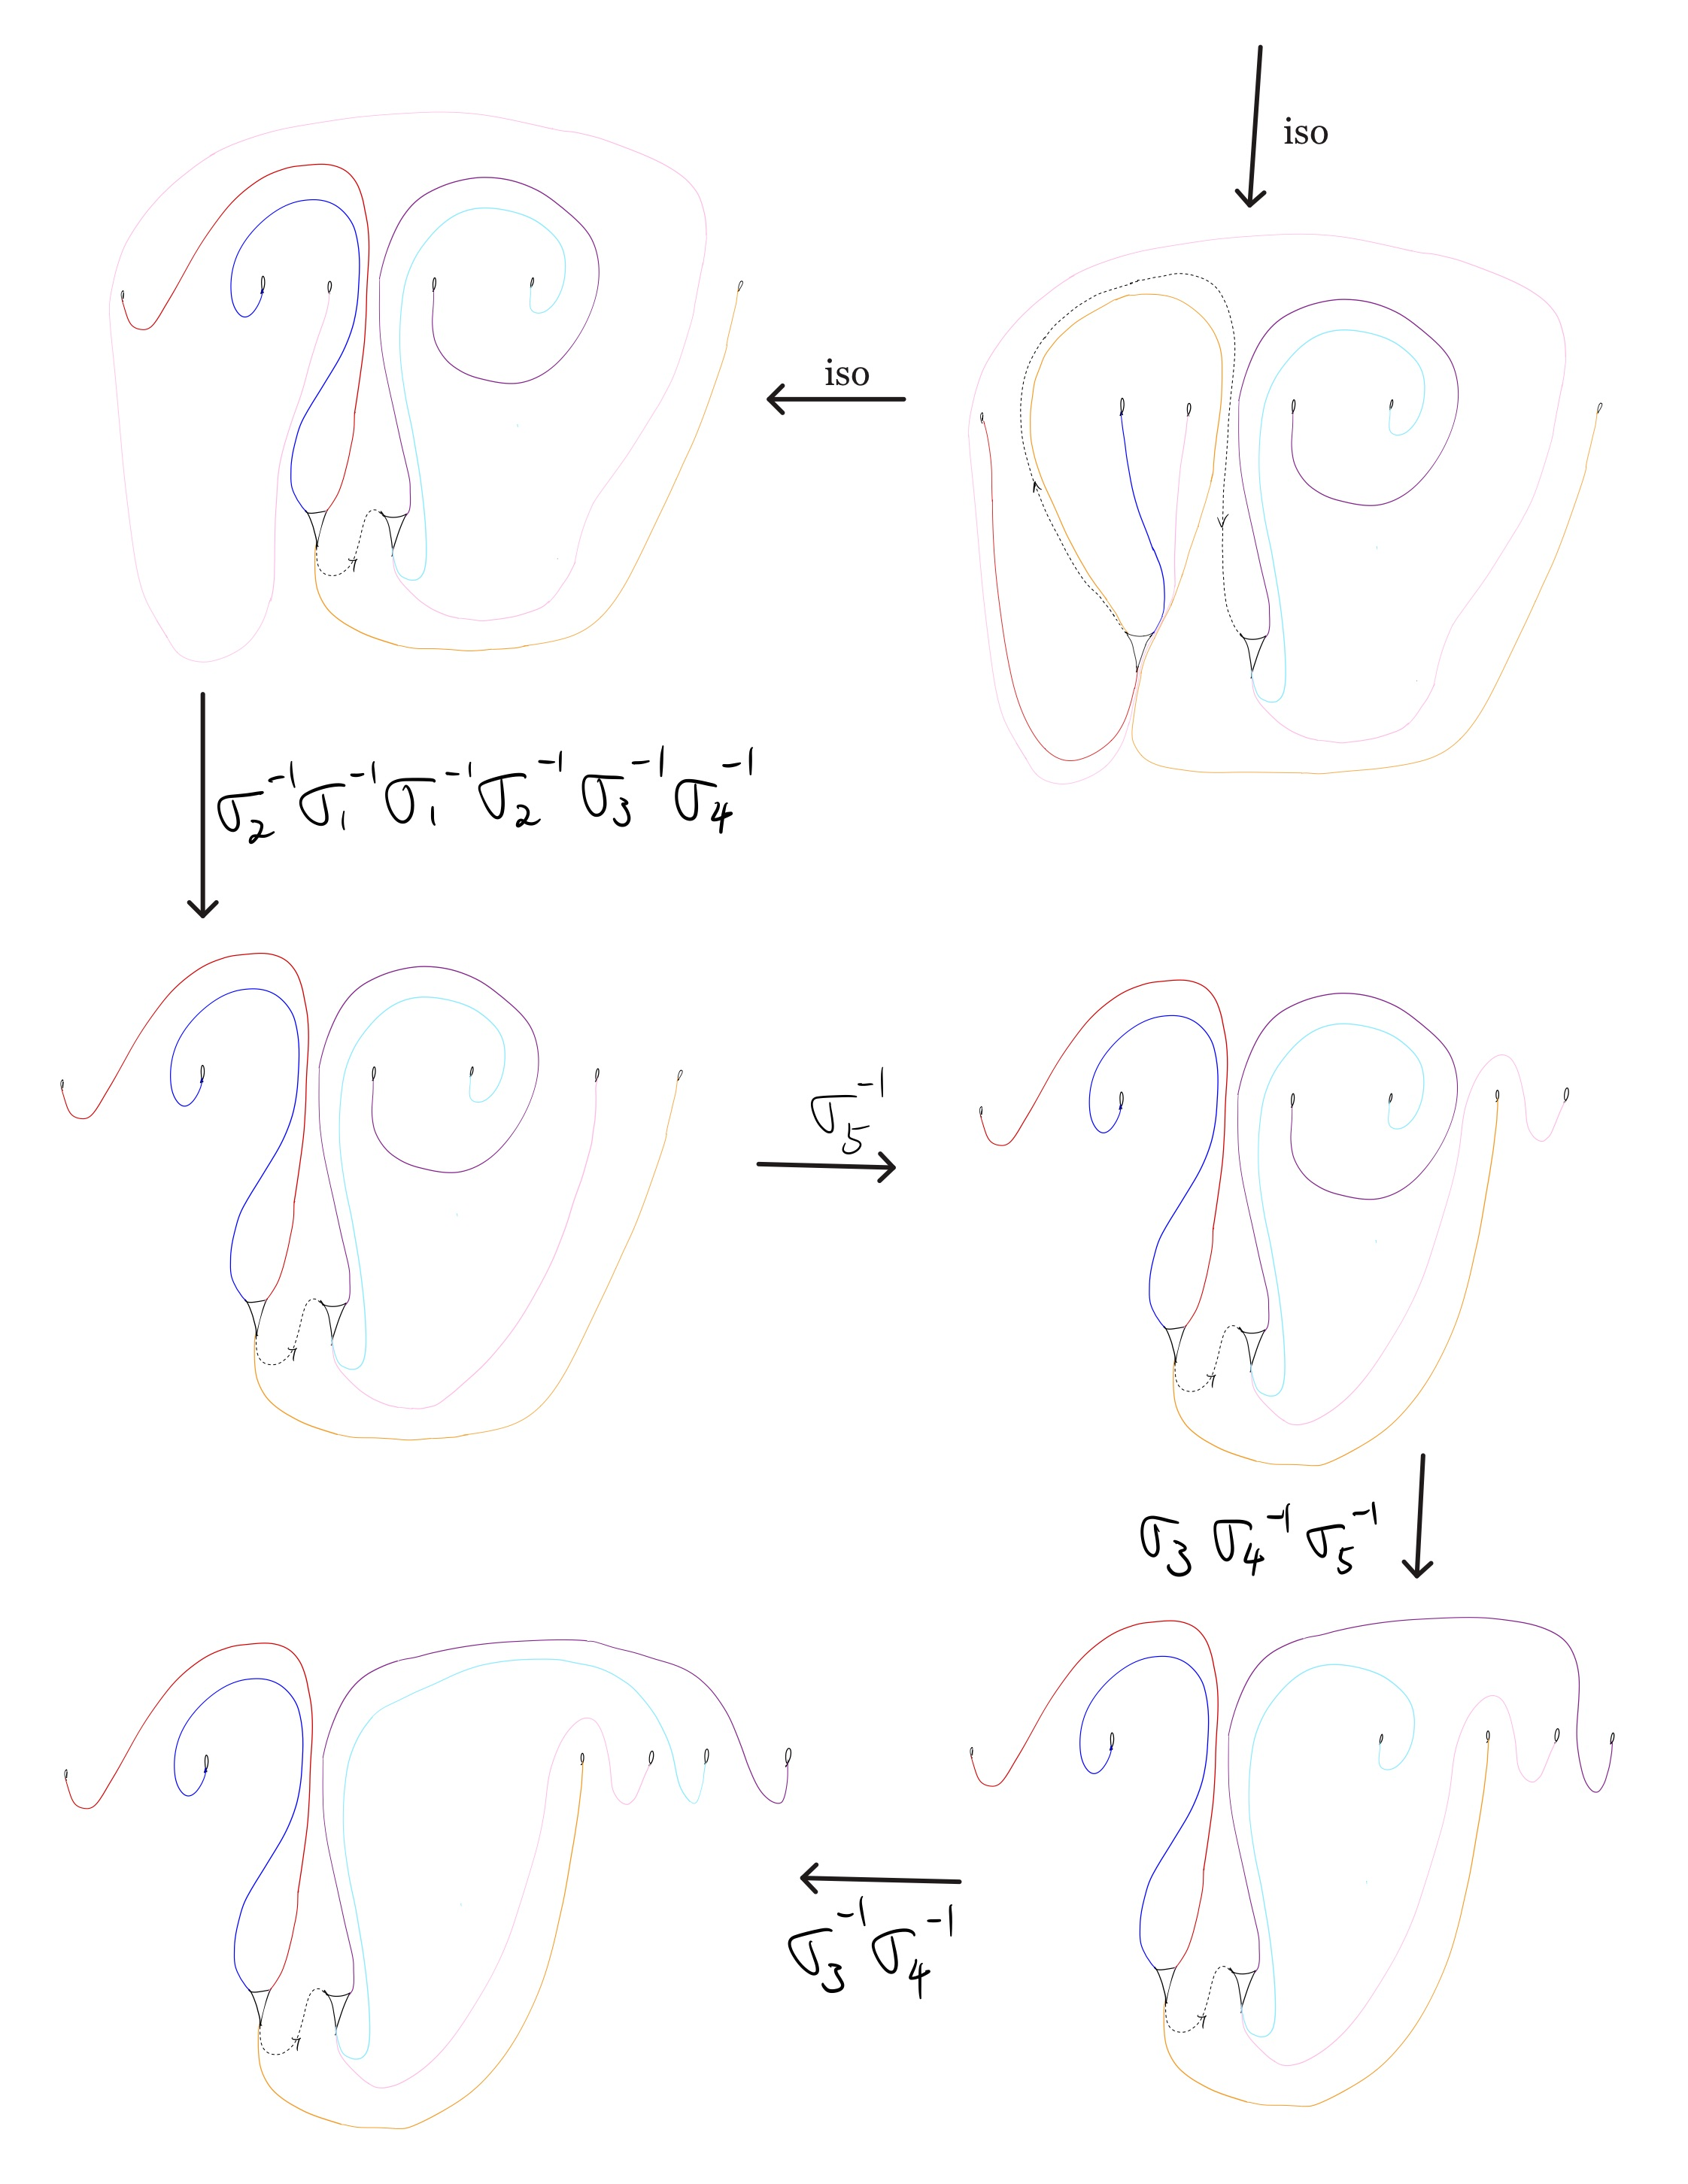
\includegraphics[width=\linewidth, height=0.45\textheight, keepaspectratio]{figures_braid/figures_track_1/Track 1 Braid 14 Sybaritic-3.jpg}
    \caption{This sequence shows the inverse of the braid $b_{14}^1$ carries Train Track Candidate Family 14.}
    \label{fig:track1_braid_b1_14}
\end{figure*}

\clearpage

\section{Candidate Family 15 (Leverage)}\label{sec:track1_leverage}
Train Track Map Candidate Family 15 of Track 1 is shown in Figure \ref{fig:track1_braid_b1_15_map}. See \ref{Leverage} for details.

\begin{figure*}[ht]
    \centering
    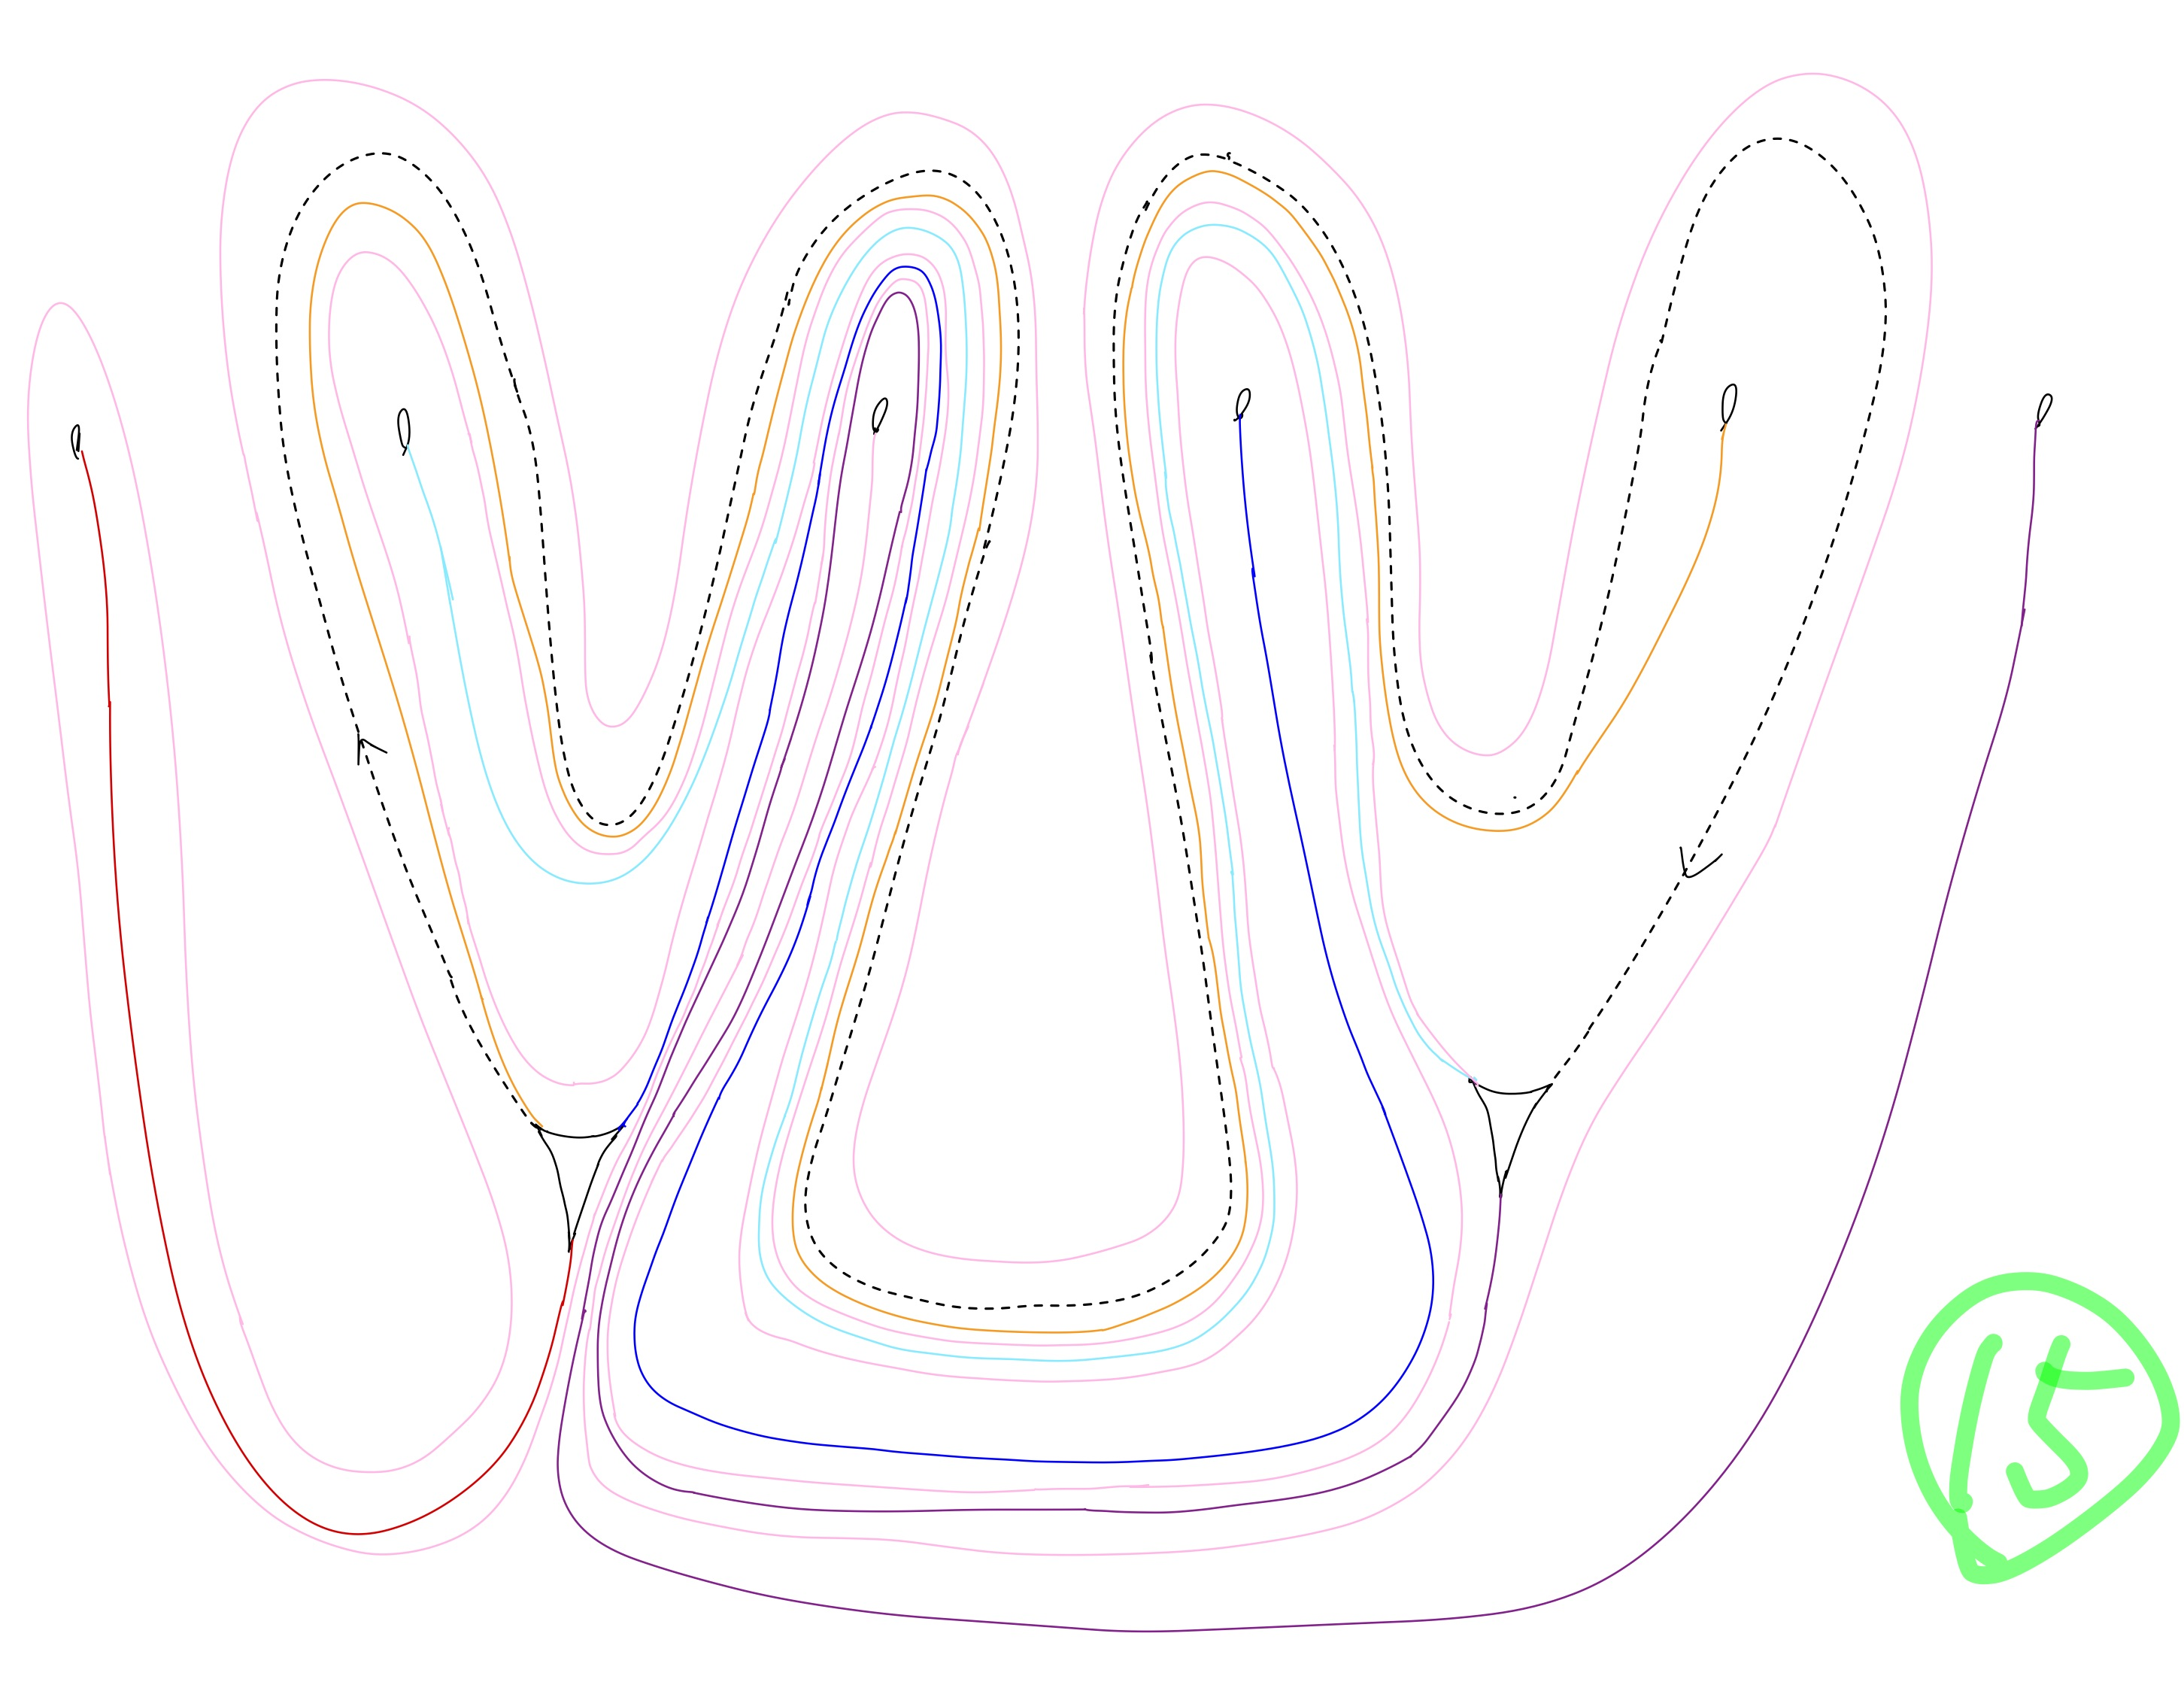
\includegraphics[width=\linewidth, height=0.45\textheight, keepaspectratio]{figures_braid/figures_track_1/Track 1 Braid 15 Leverage-1.jpg}
    \caption{Train Track Map Candidate Family 15 (Leverage) of Track 1.}
    \label{fig:track1_braid_b1_15_map}
\end{figure*}

The inverse of the following braid carries this family of train track maps:
\[
b_{15}^1 = \sigma_{4} \sigma_{3} \sigma_{2} \sigma_{3}^{-1} \sigma_{4}^{-1} \sigma_{3} \sigma_{4} \sigma_{4} \sigma_{3} \sigma_{2} \sigma_{1} \sigma_{1} \sigma_{3}^{-1} \sigma_{2} \sigma_{3} \sigma_{1}^{-1} \sigma_{2}^{-1} \sigma_{1}^{-1} \sigma_{5} \sigma_{4} \sigma_{5}
\]

This is shown in Figure \ref{fig:track1_braid_b1_15}.

\begin{figure*}[p]
    \centering
    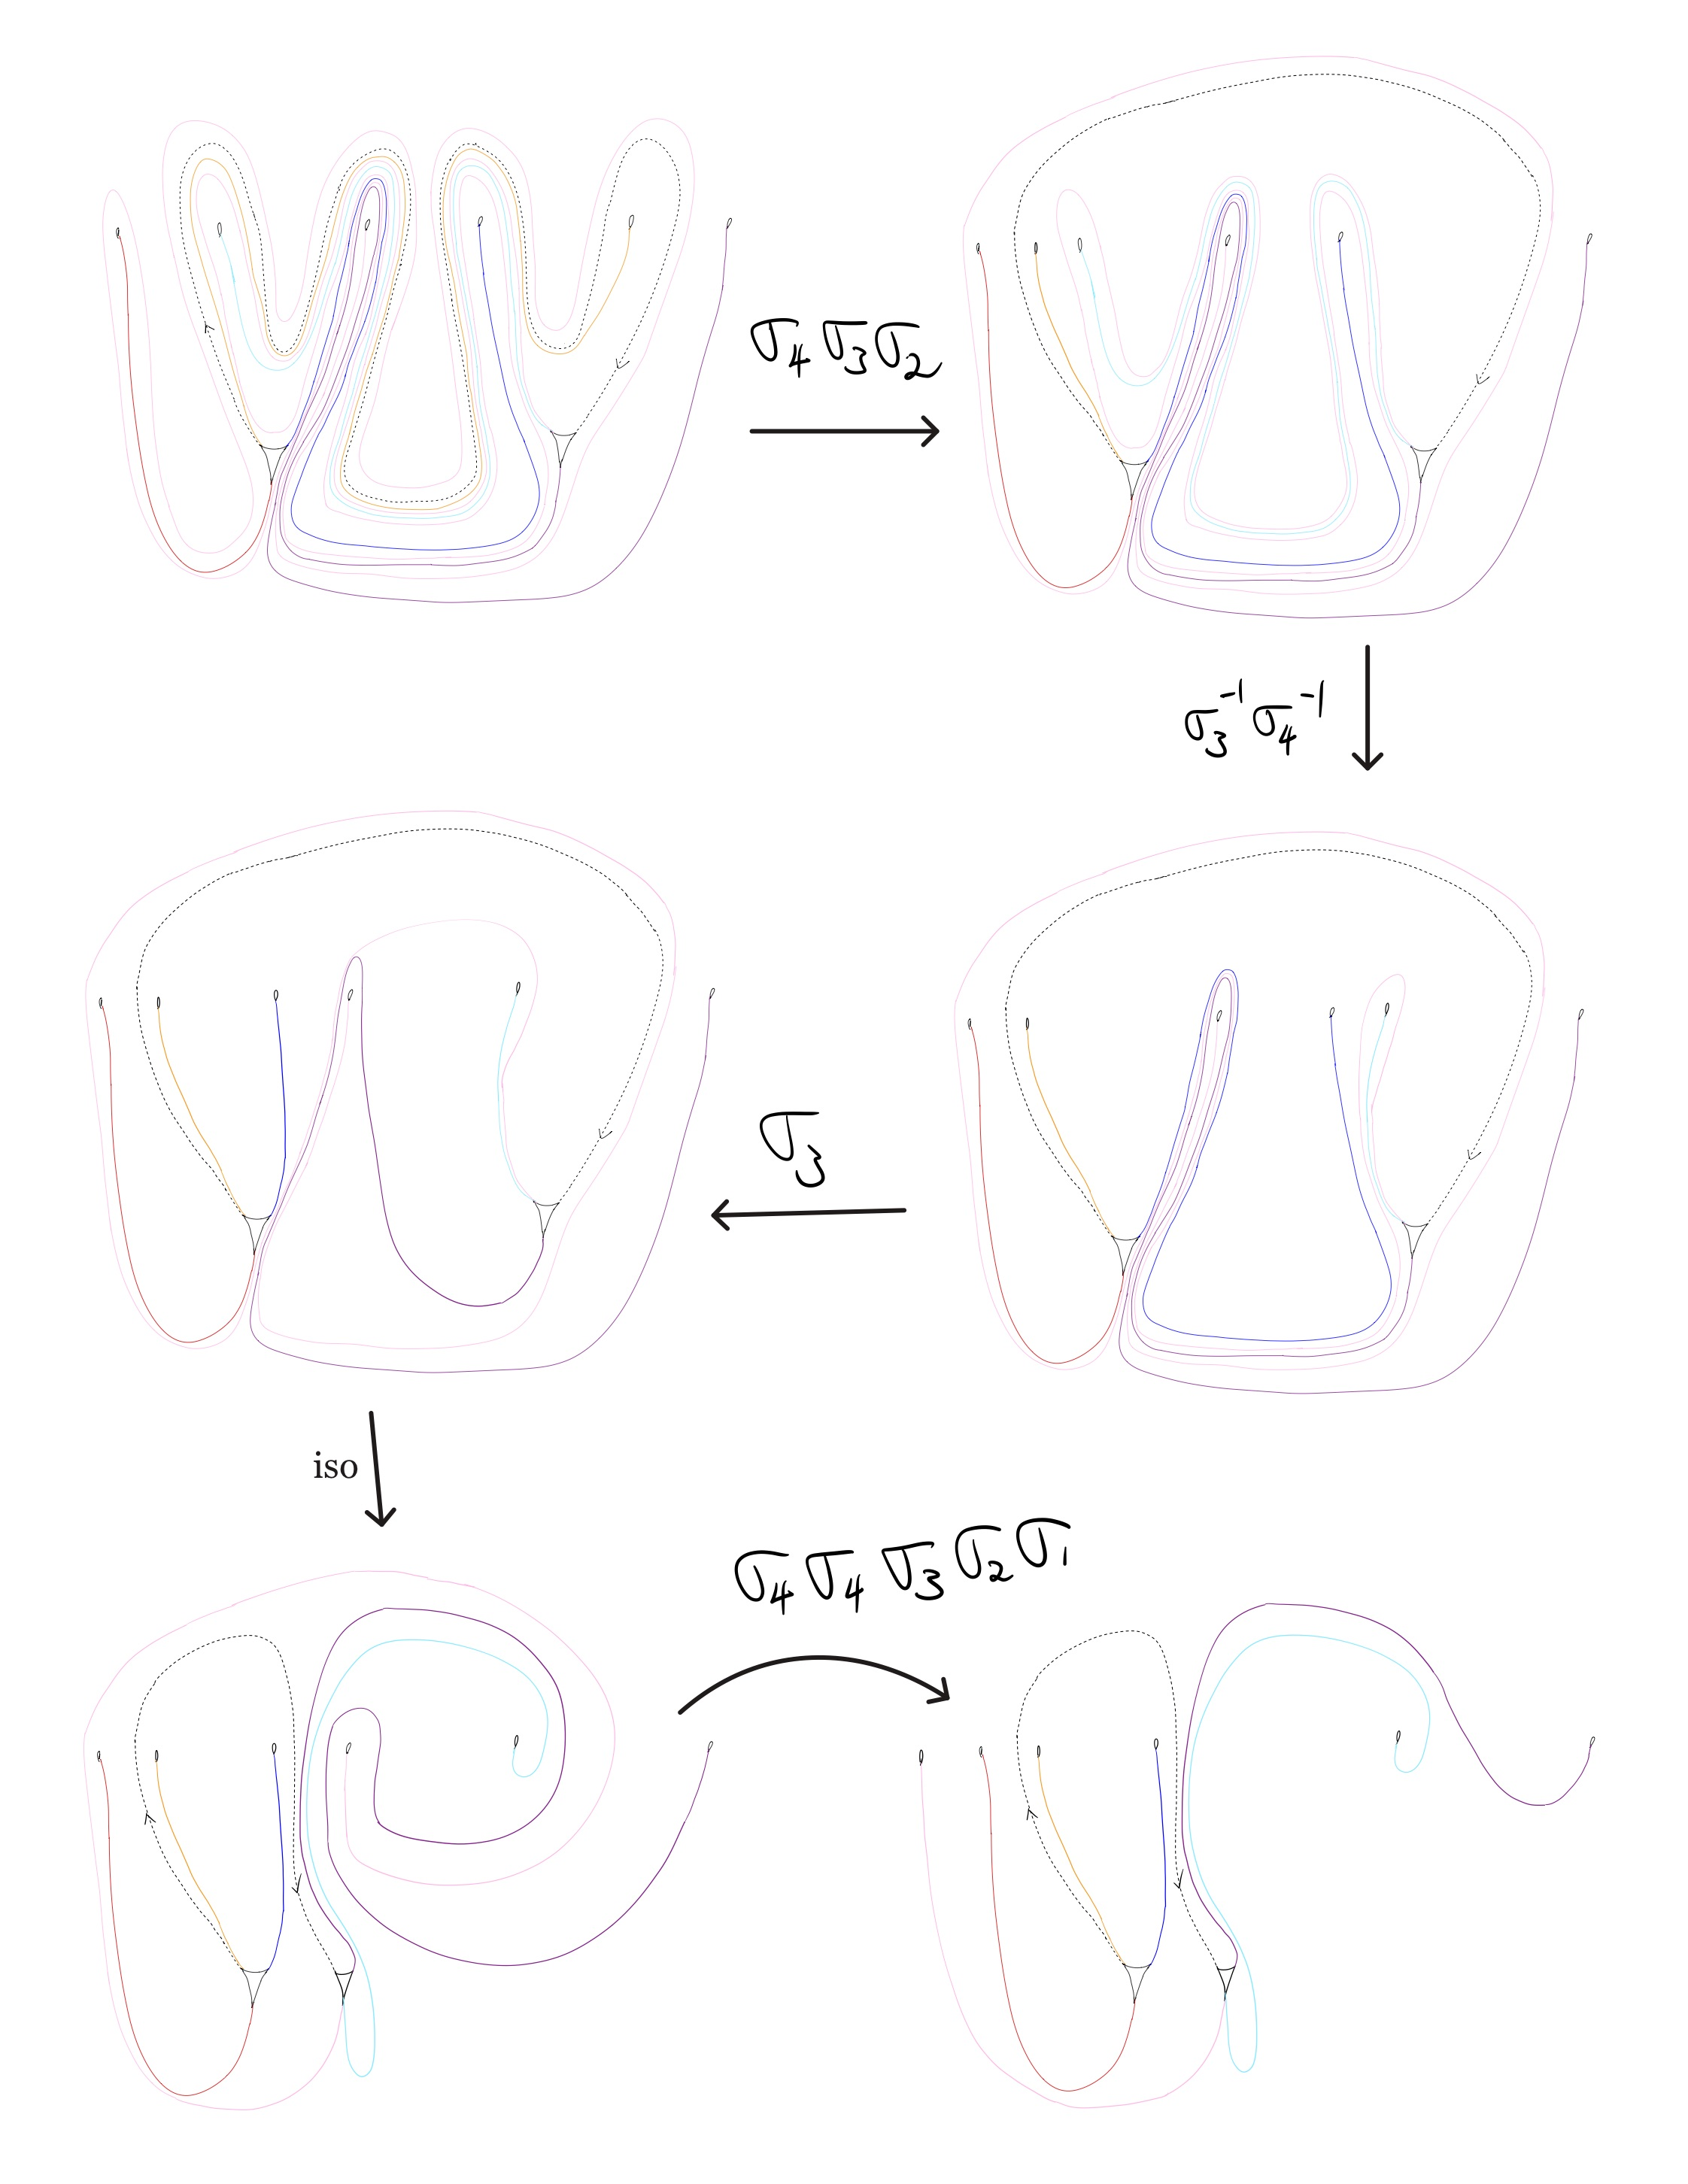
\includegraphics[width=\linewidth, height=0.45\textheight, keepaspectratio]{figures_braid/figures_track_1/Track 1 Braid 15 Leverage-2.jpg}\\
    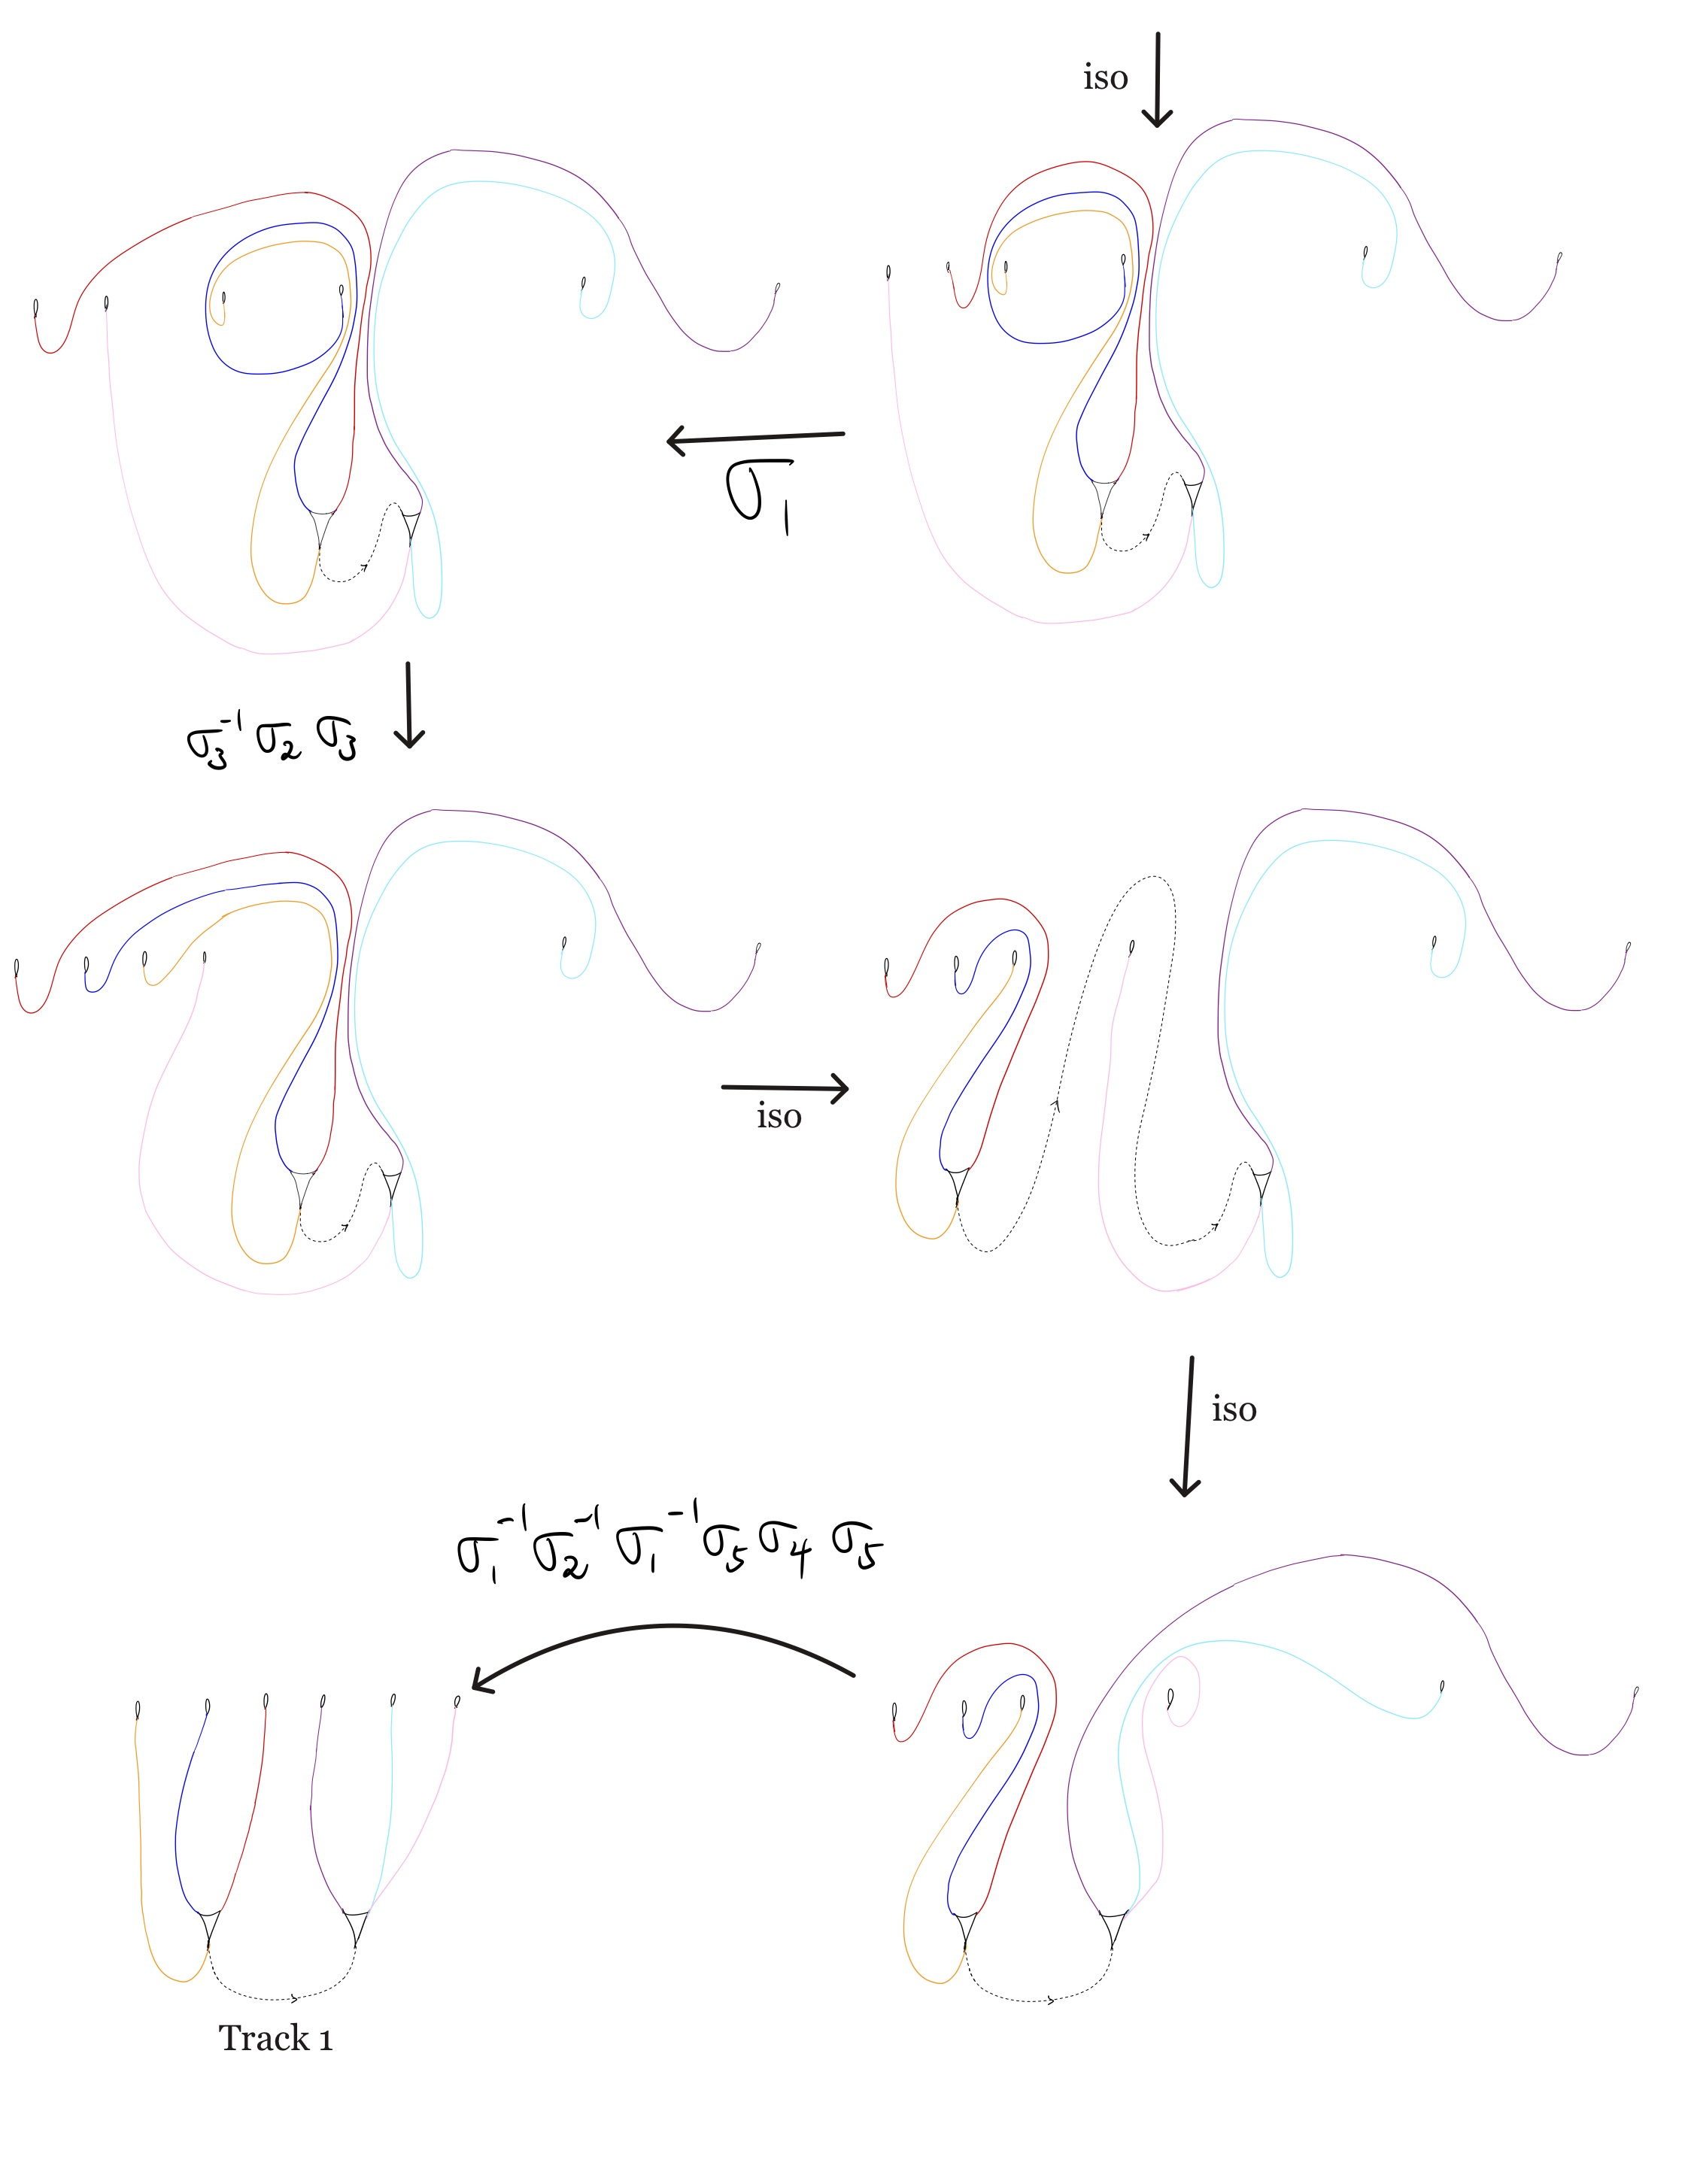
\includegraphics[width=\linewidth, height=0.45\textheight, keepaspectratio]{figures_braid/figures_track_1/Track 1 Braid 15 Leverage-3.jpg}
    \caption{This sequence shows the inverse of the braid $b_{15}^1$ carries Train Track Candidate Family 15.}
    \label{fig:track1_braid_b1_15}
\end{figure*}

\clearpage

\section{Candidate Family 16 (Guddle)}\label{sec:track1_guddle}
Train Track Map Candidate Family 16 of Track 1 is shown in Figure \ref{fig:track1_braid_b1_16_map}. See \ref{Guddle} for details.

\begin{figure*}[ht]
    \centering
    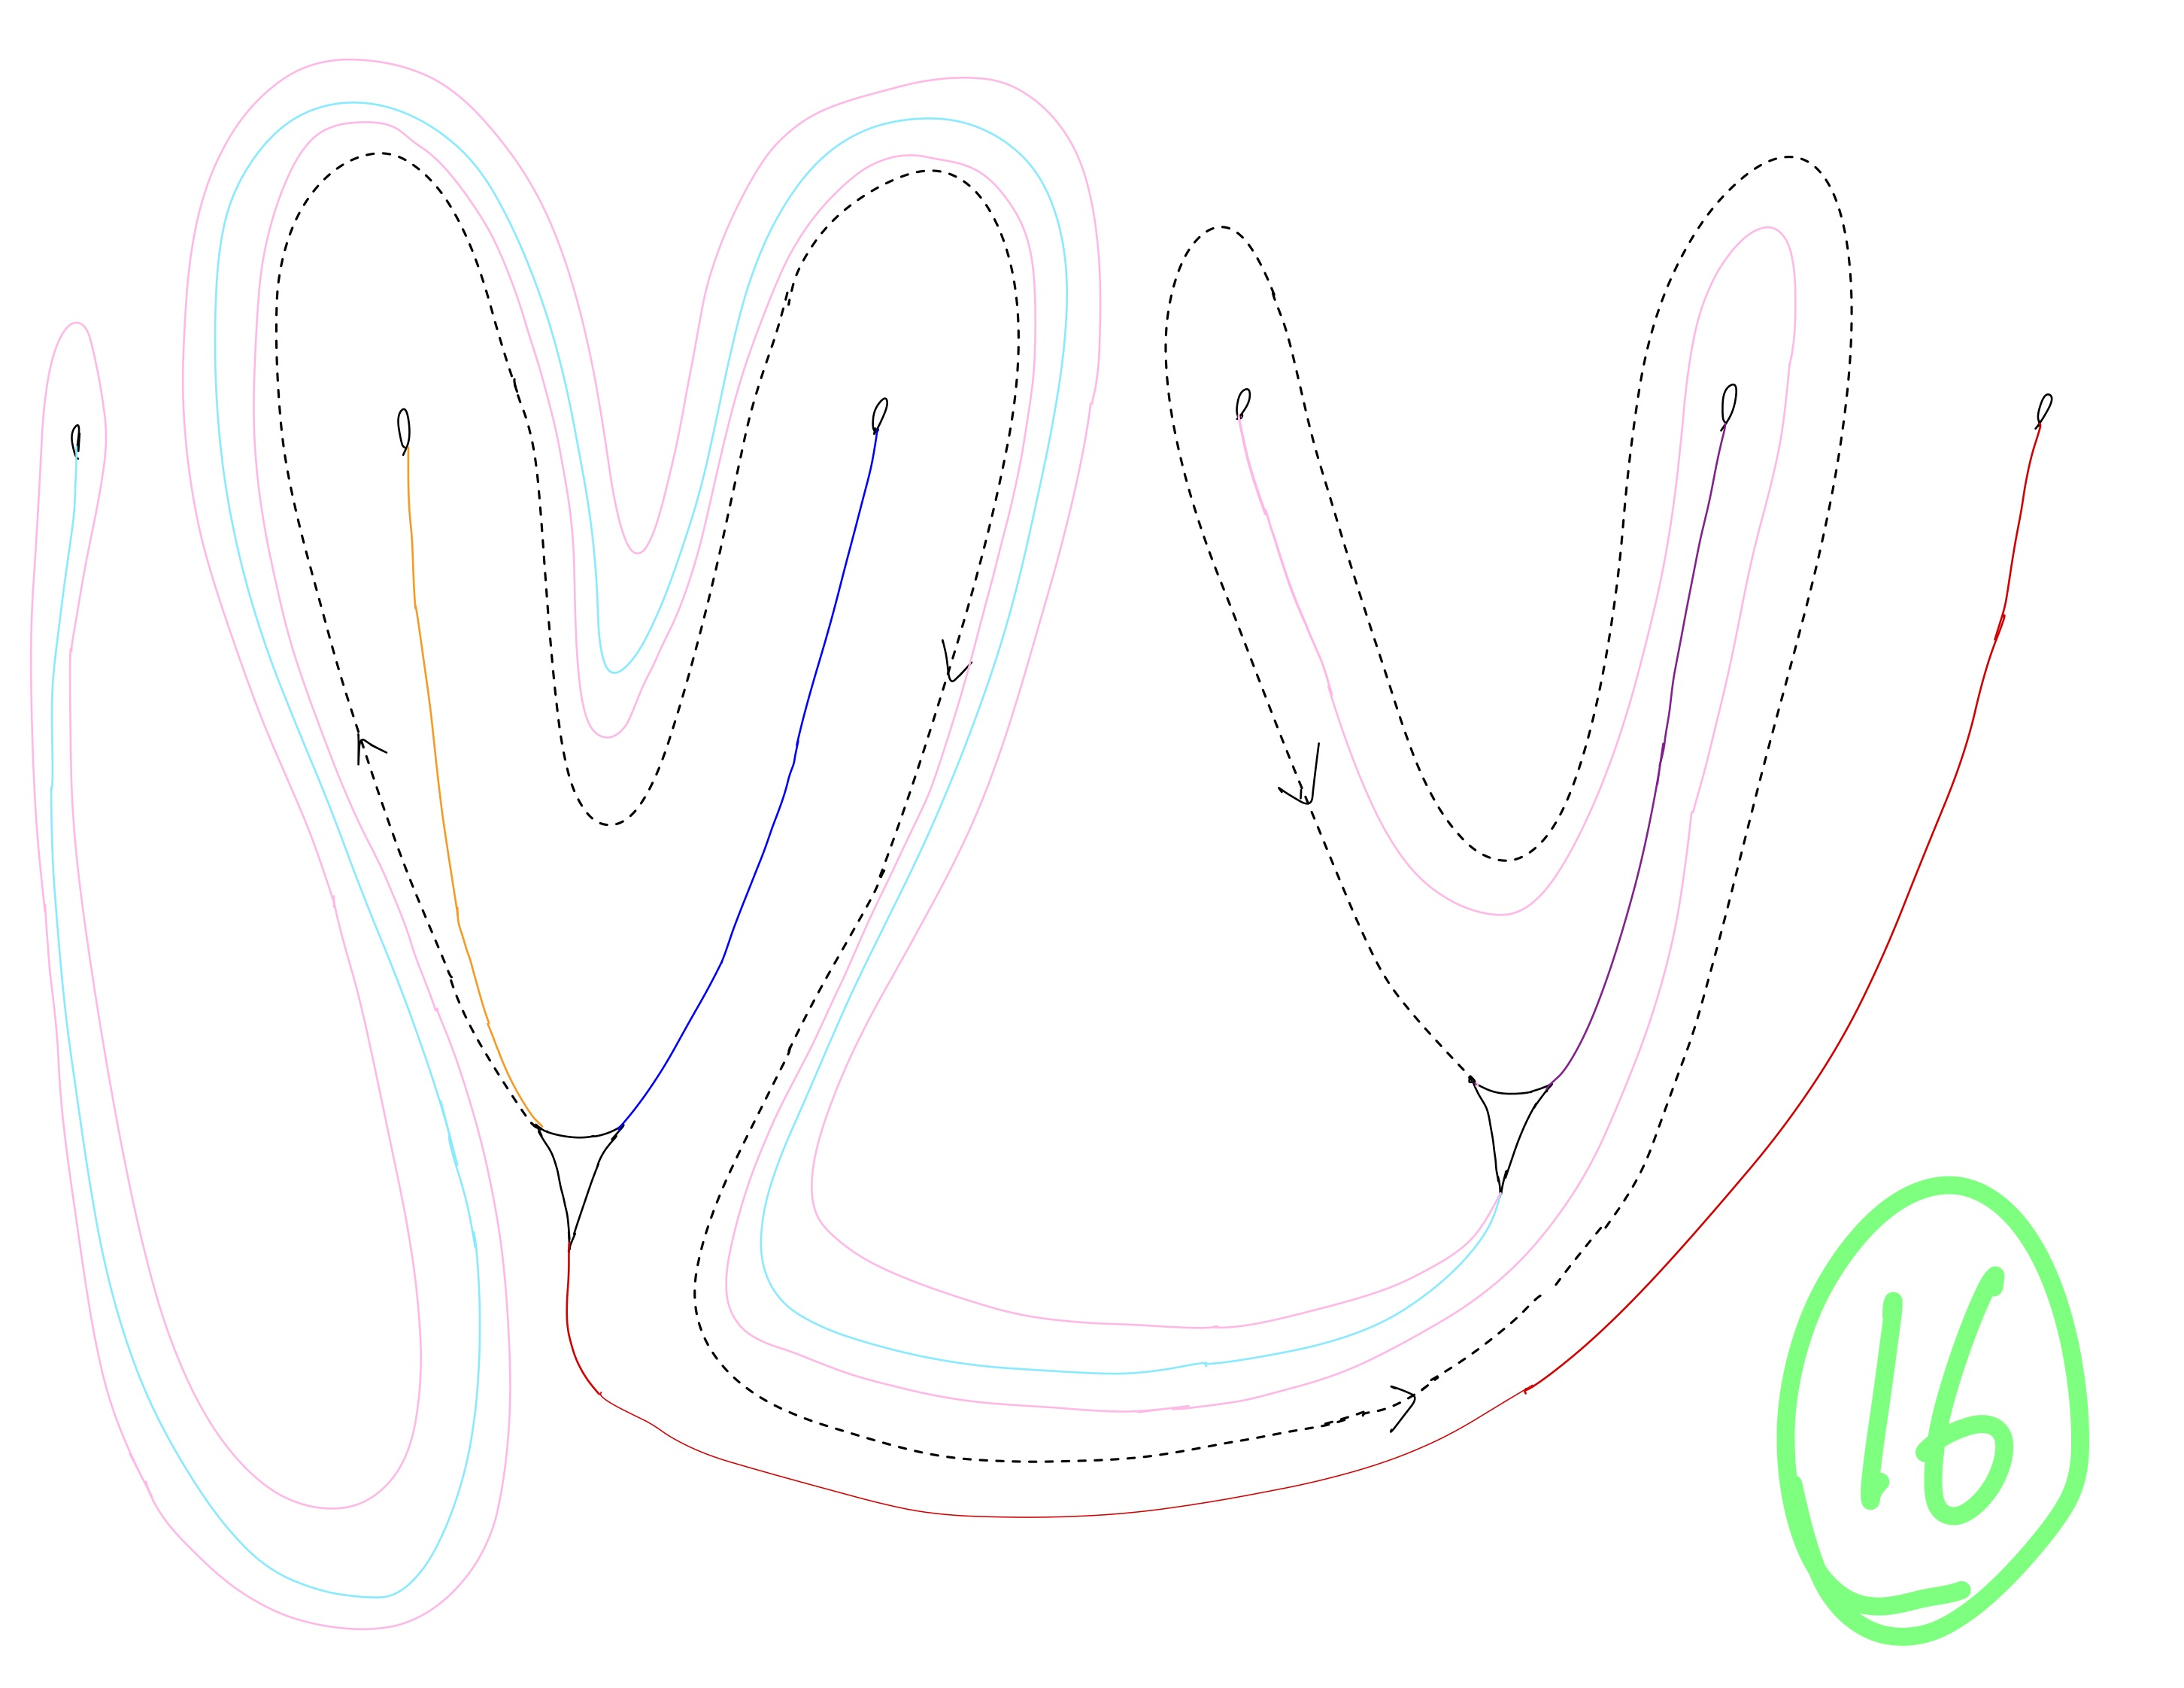
\includegraphics[width=\linewidth, height=0.45\textheight, keepaspectratio]{figures_braid/figures_track_1/Track 1 Braid 16 Guddle-1.jpg}
    \caption{Train Track Map Candidate Family 16 (Guddle) of Track 1.}
    \label{fig:track1_braid_b1_16_map}
\end{figure*}

The inverse of the following braid carries this family of train track maps:
\[
b_{16}^1 = \sigma_{4}^{-1} \sigma_{1}^{-1} \sigma_{2}^{-1} \sigma_{3}^{-1} \sigma_{4}^{-1} \sigma_{3}^{-1} \sigma_{3}^{-1} \sigma_{4}^{-1} \sigma_{1}^{-1} \sigma_{1}^{-1} \sigma_{5}^{-1} \sigma_{4}^{-1} \sigma_{3}^{-1} \sigma_{2}^{-1} \sigma_{1}^{-1} \sigma_{1}^{-1} \sigma_{2}^{-1}
\]

This is shown in Figure \ref{fig:track1_braid_b1_16}.

\begin{figure*}[p]
    \centering
    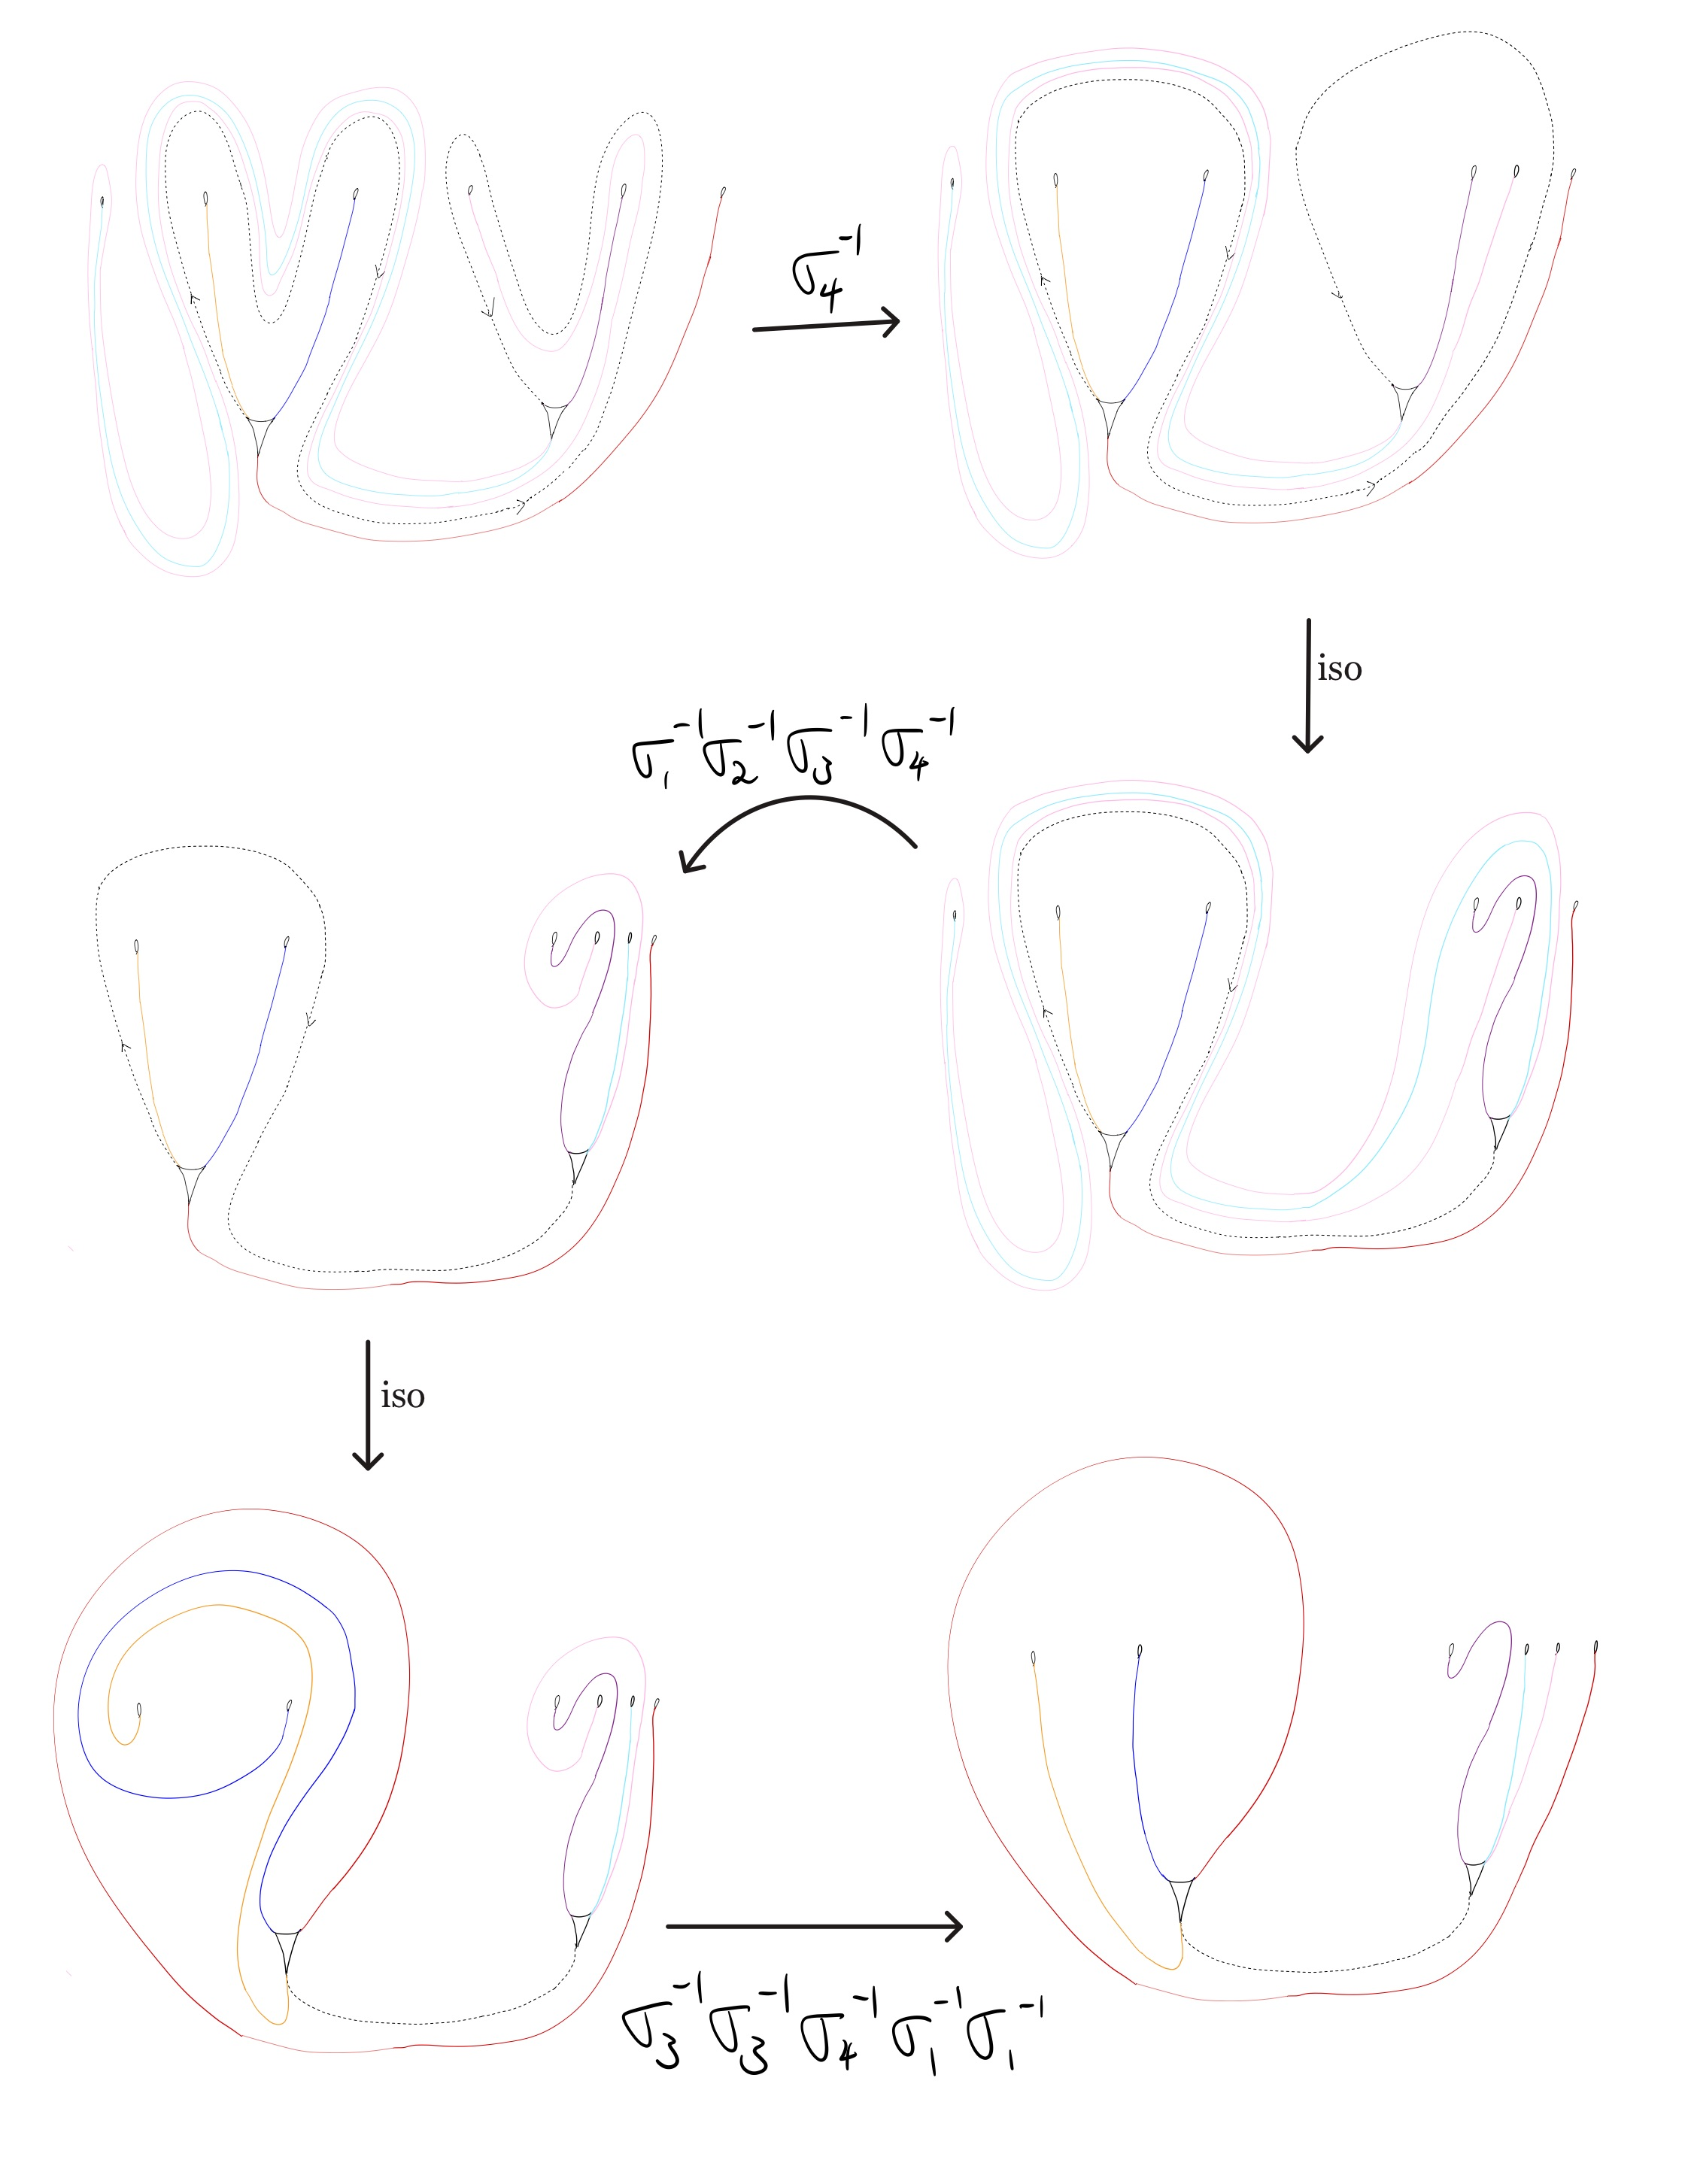
\includegraphics[width=\linewidth, height=0.45\textheight, keepaspectratio]{figures_braid/figures_track_1/Track 1 Braid 16 Guddle-2.jpg}\\
    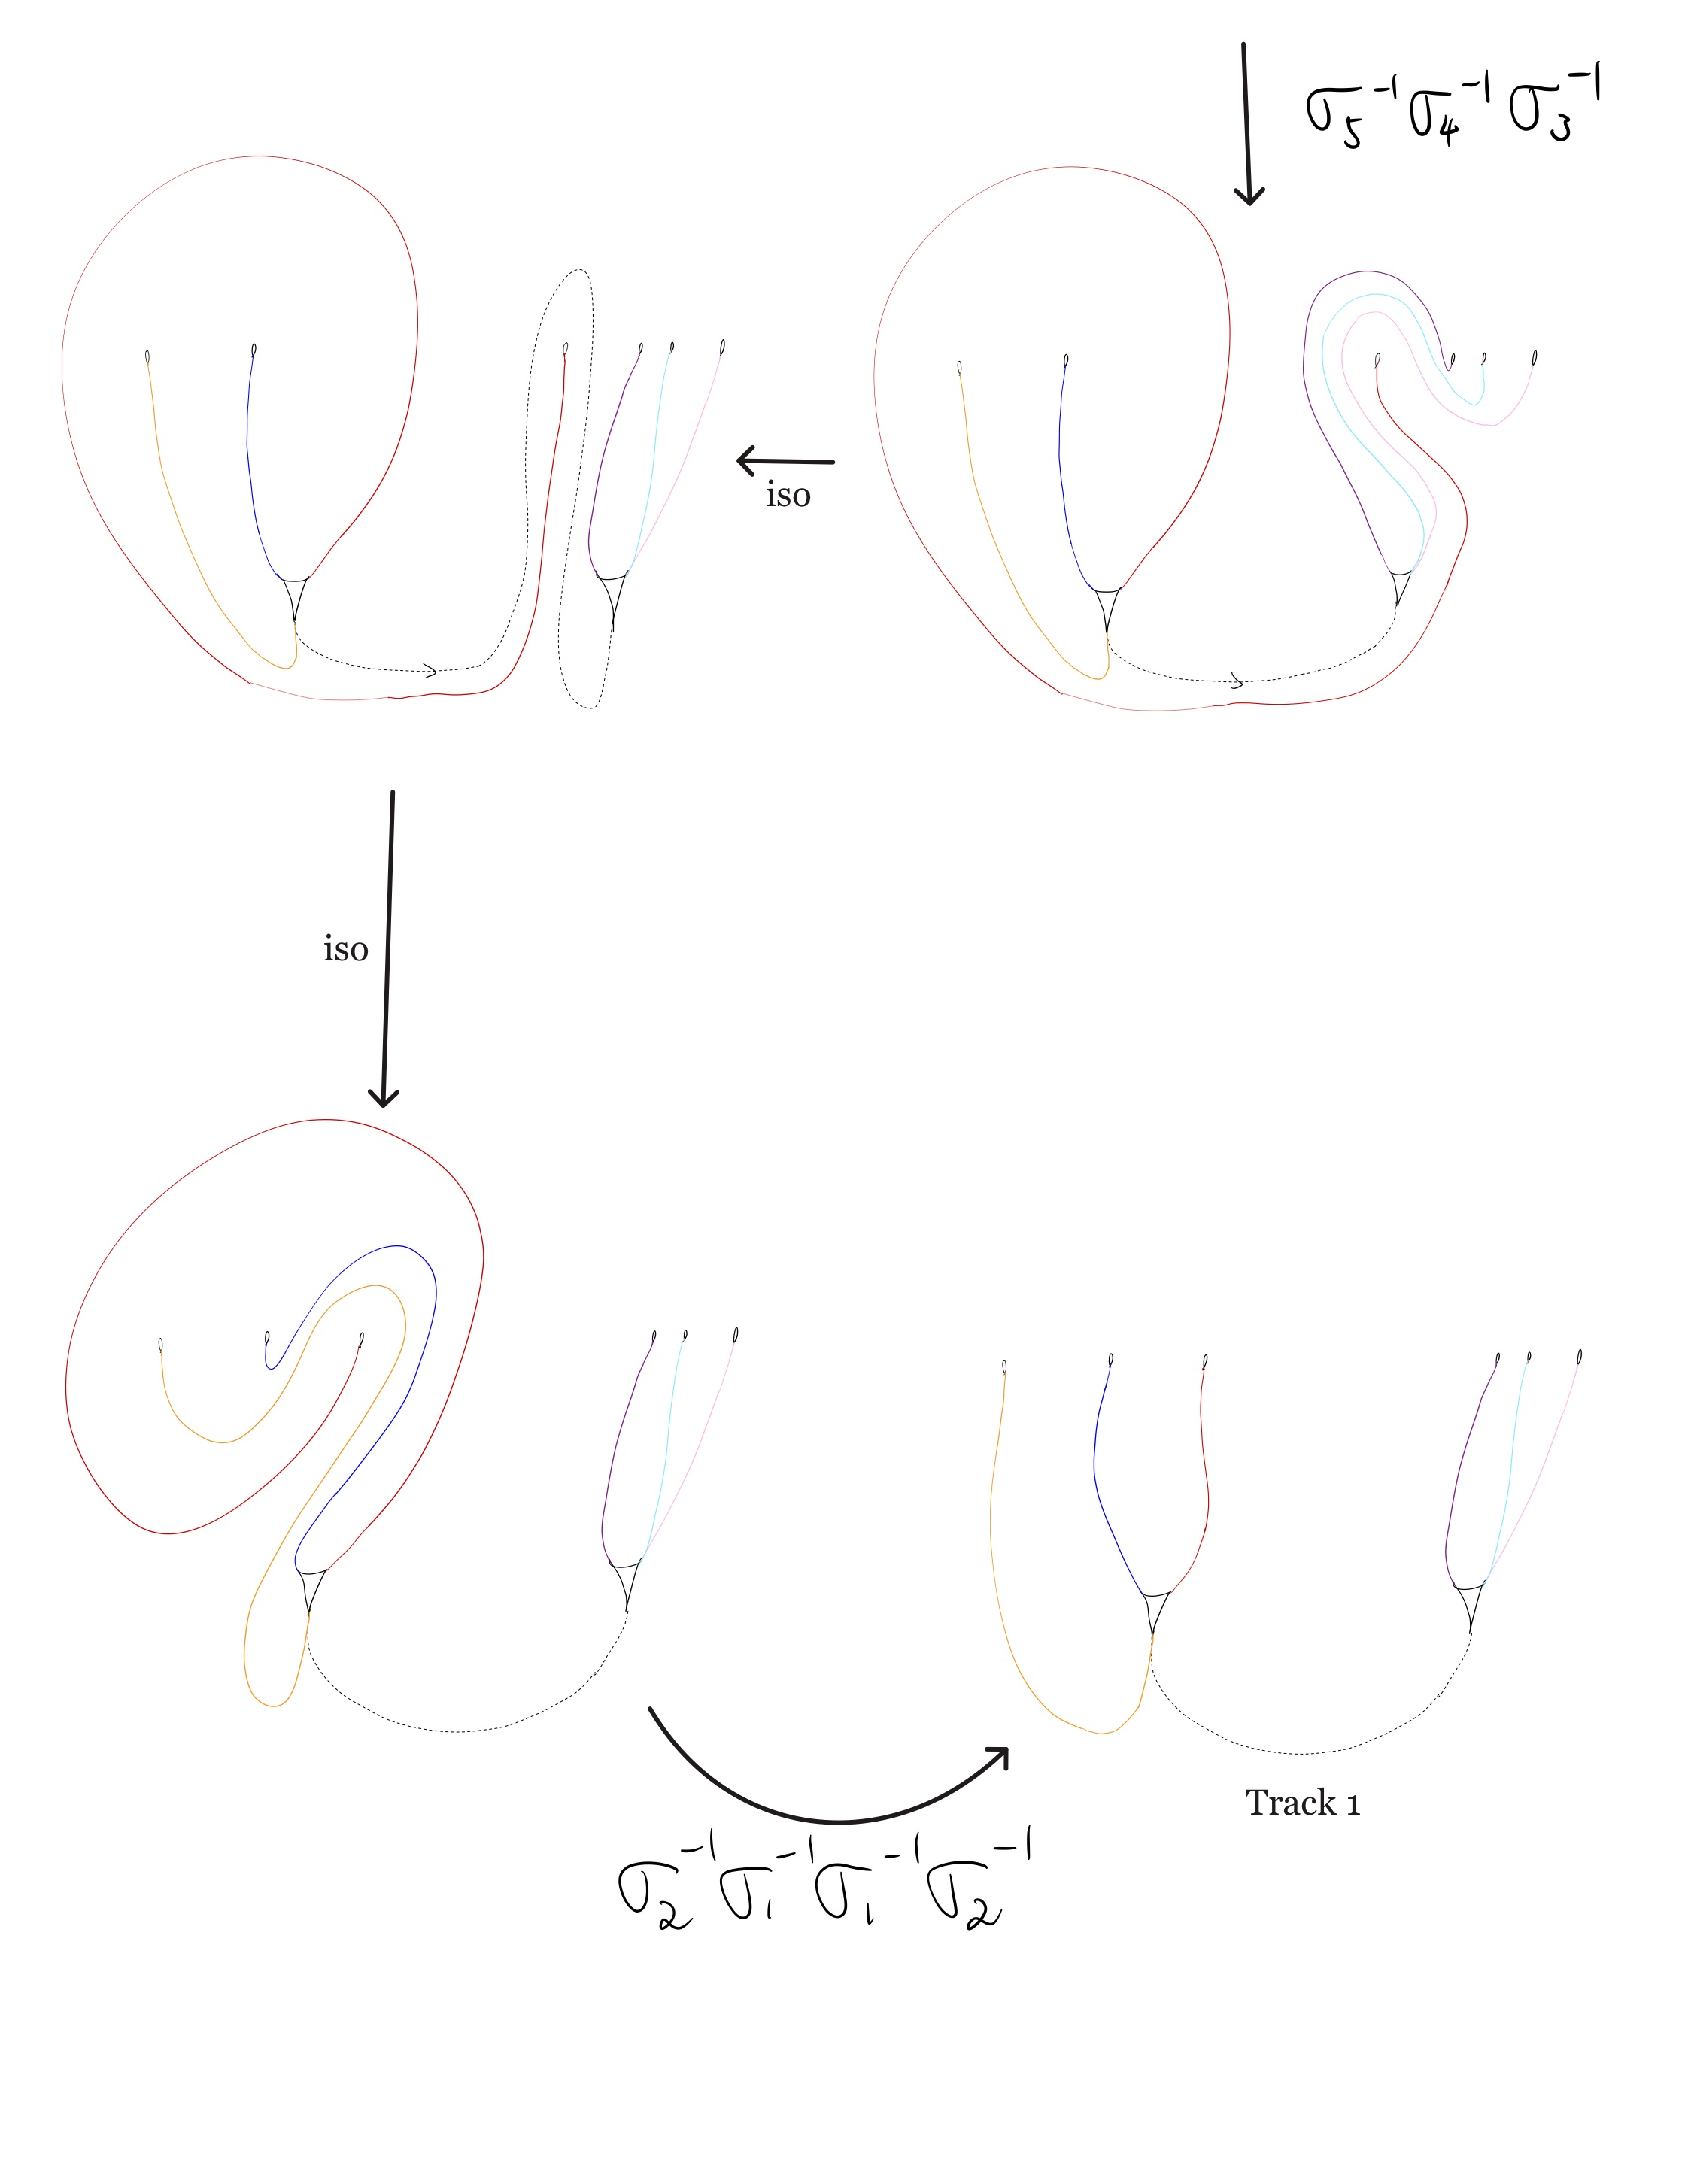
\includegraphics[width=\linewidth, height=0.45\textheight, keepaspectratio]{figures_braid/figures_track_1/Track 1 Braid 16 Guddle-3.jpg}
    \caption{This sequence shows the inverse of the braid $b_{16}^1$ carries Train Track Candidate Family 16.}
    \label{fig:track1_braid_b1_16}
\end{figure*}

\clearpage

\section{Candidate Family 17 (Popjoy)}\label{sec:track1_popjoy}
Train Track Map Candidate Family 17 of Track 1 is shown in Figure \ref{fig:track1_braid_b1_17_map}. See \ref{Popjoy} for details.

\begin{figure*}[ht]
    \centering
    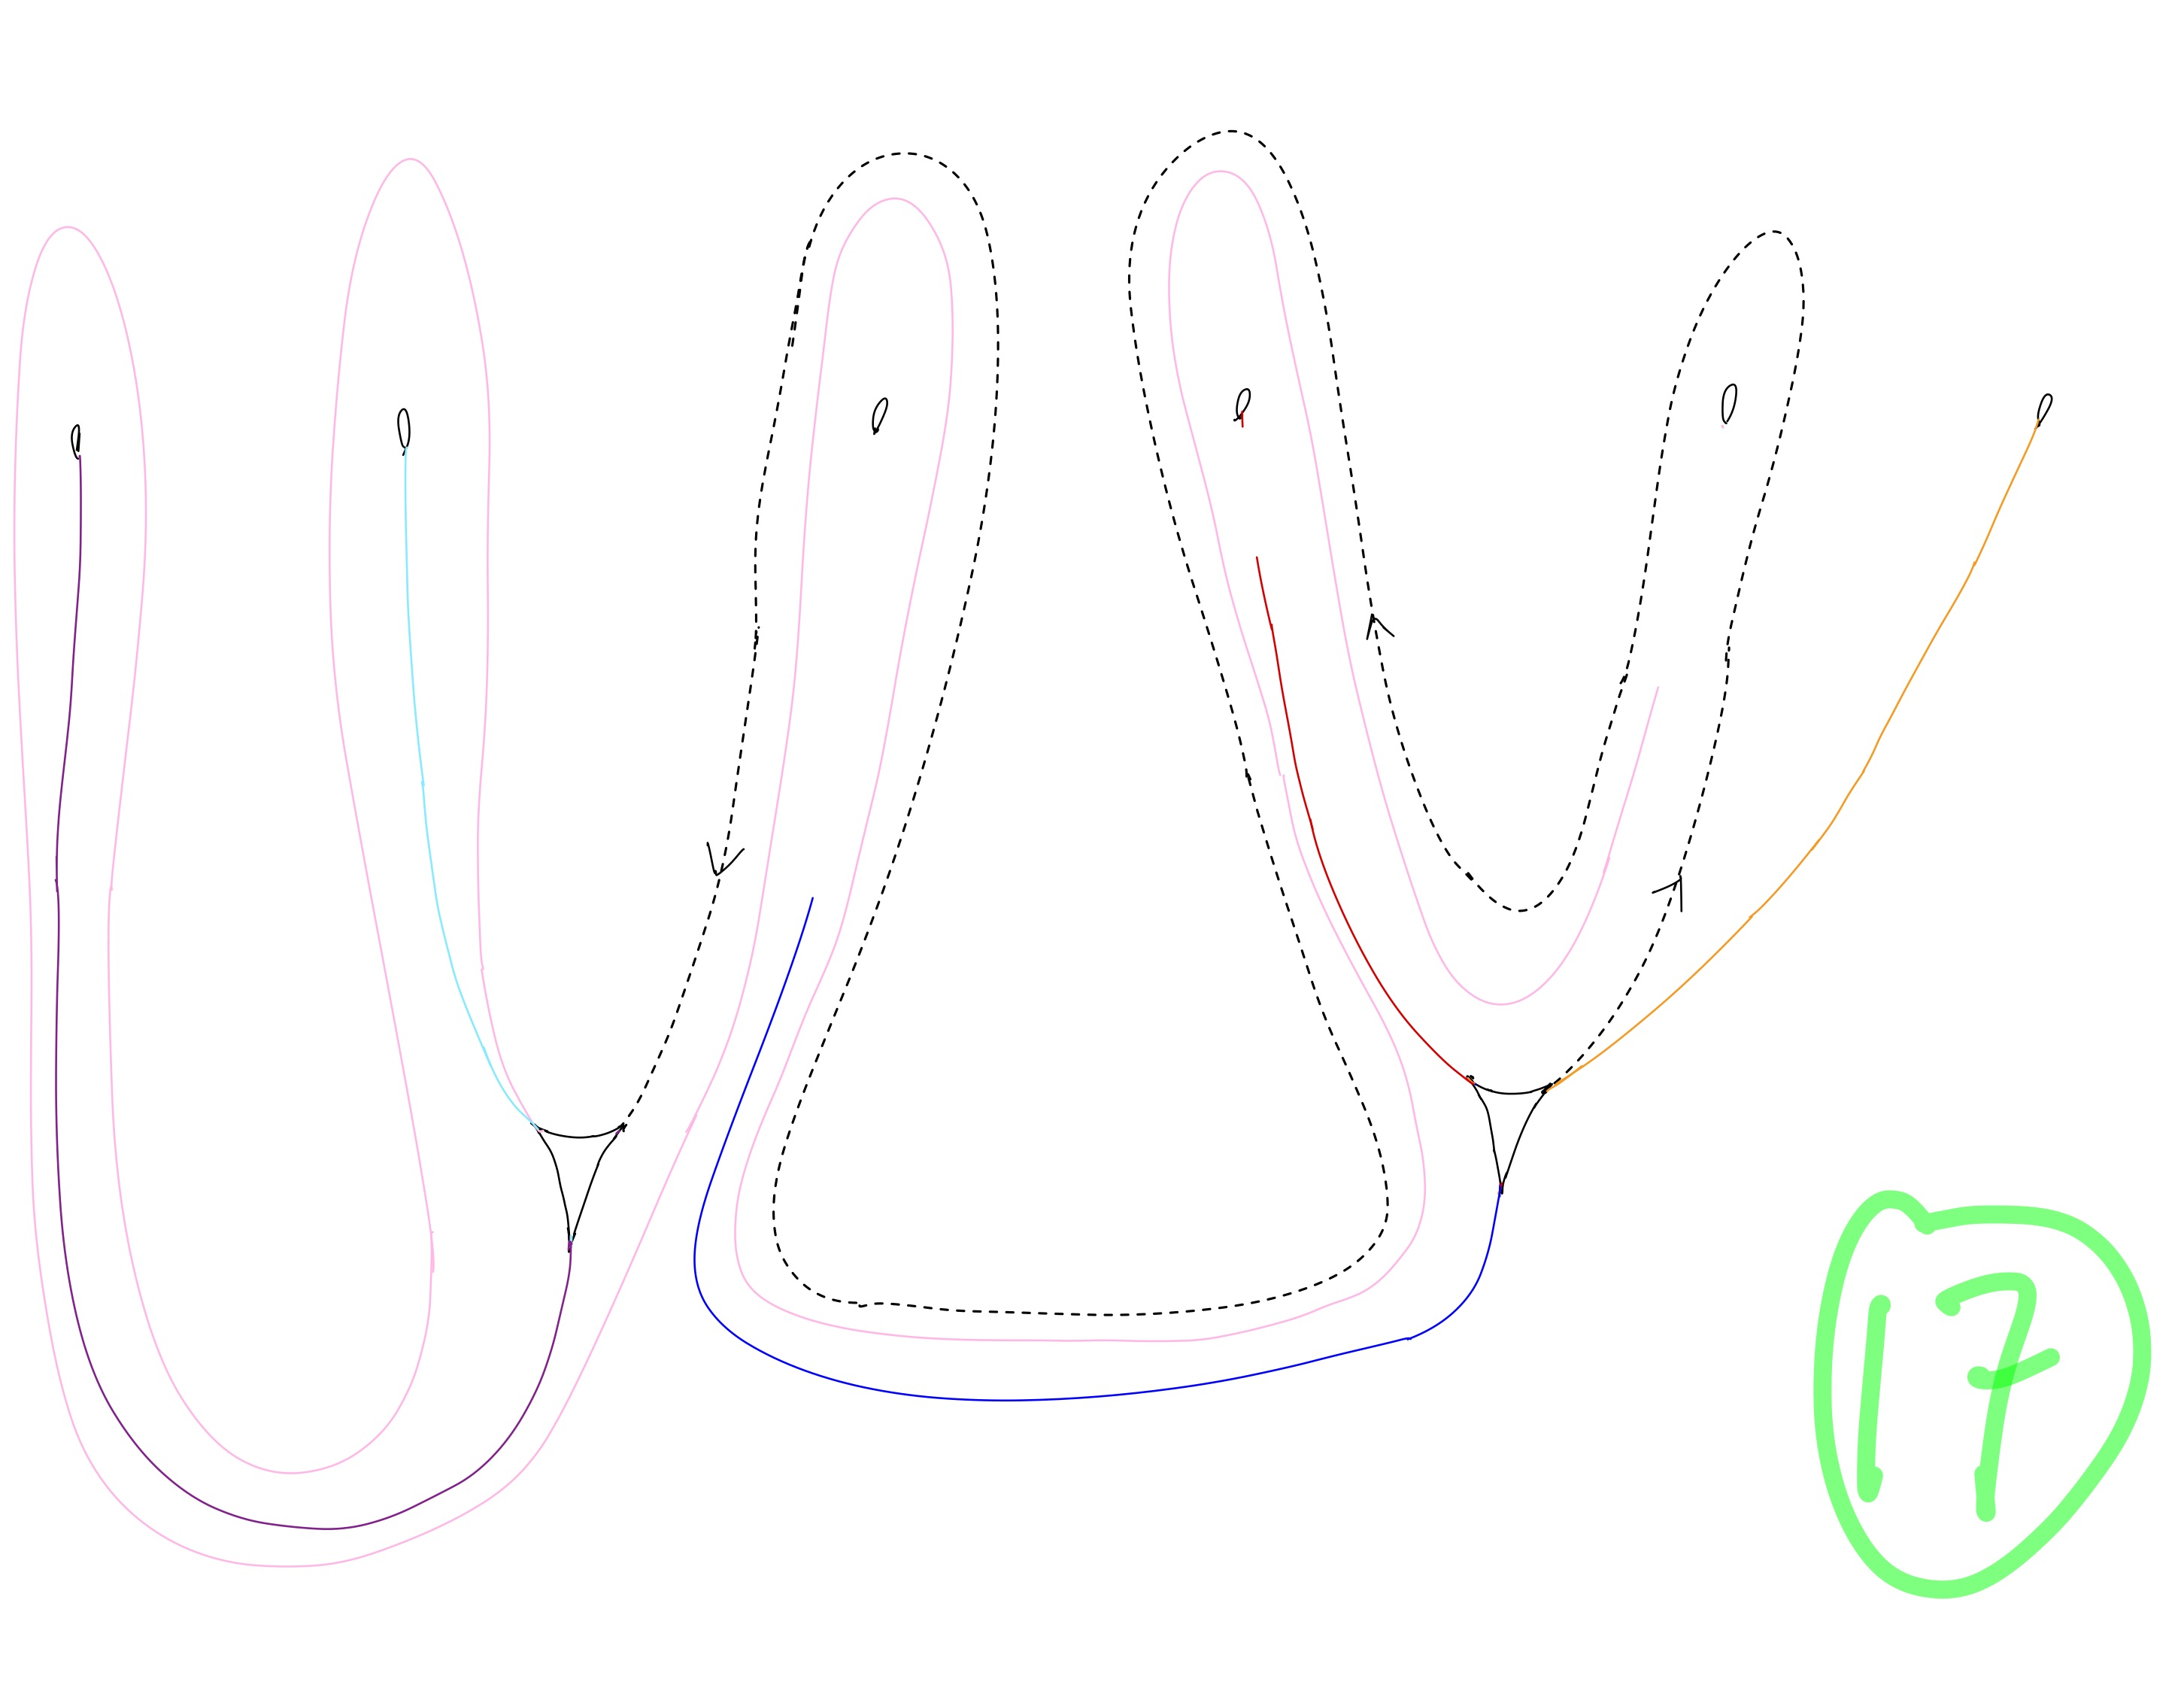
\includegraphics[width=\linewidth, height=0.45\textheight, keepaspectratio]{figures_braid/figures_track_1/Track 1 Braid 17 Popjoy-1.jpg}
    \caption{Train Track Map Candidate Family 17 (Popjoy) of Track 1.}
    \label{fig:track1_braid_b1_17_map}
\end{figure*}

The inverse of the following braid carries this family of train track maps:
\[
b_{17}^1 = \sigma_{4}^k \sigma_{3}^m \sigma_{2}^{-1} \sigma_{1}^{-1} \sigma_{1}^{-1} \sigma_{2}^{-1} \sigma_{5} \sigma_{4} \sigma_{5} \circ J \circ \Lambda_6
\]
where $k, m \geq 1$ ($k, m \in \mathbb{Z}$) are the twisting parameters. This is shown in Figure \ref{fig:track1_braid_b1_17}.

\begin{figure*}[p]
    \centering
    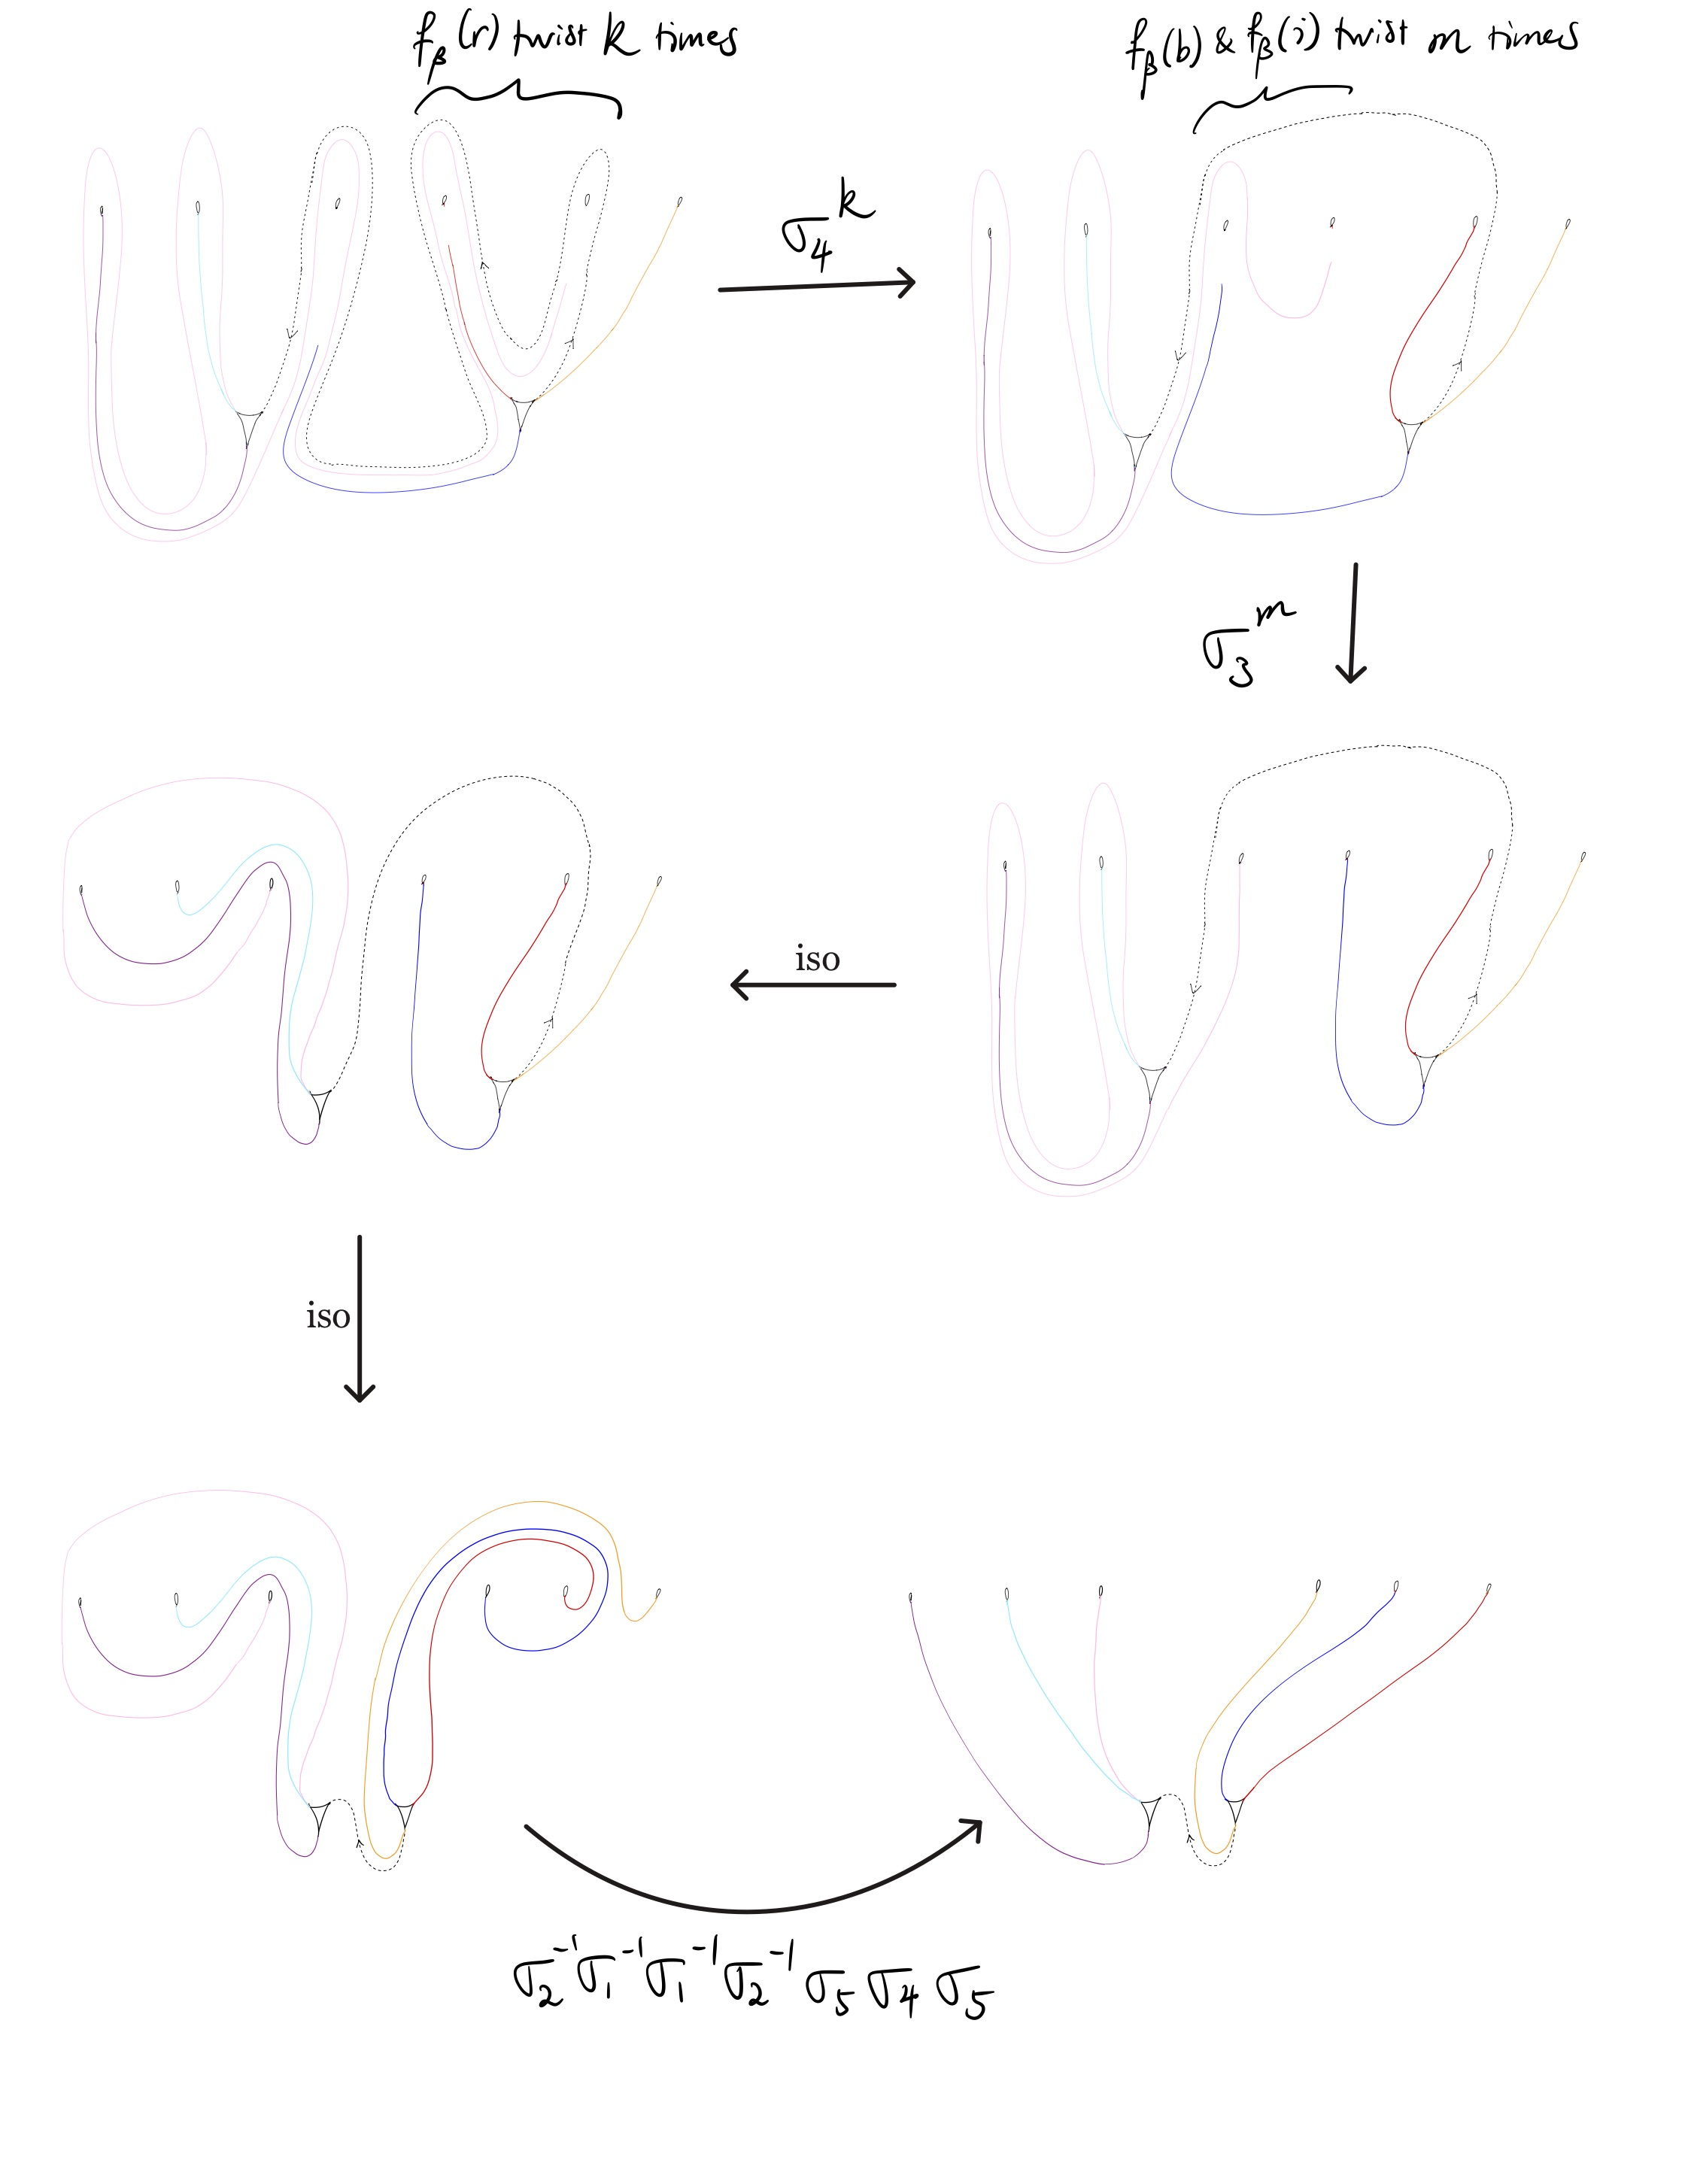
\includegraphics[width=\linewidth, height=0.45\textheight, keepaspectratio]{figures_braid/figures_track_1/Track 1 Braid 17 Popjoy-2.jpg}\\
    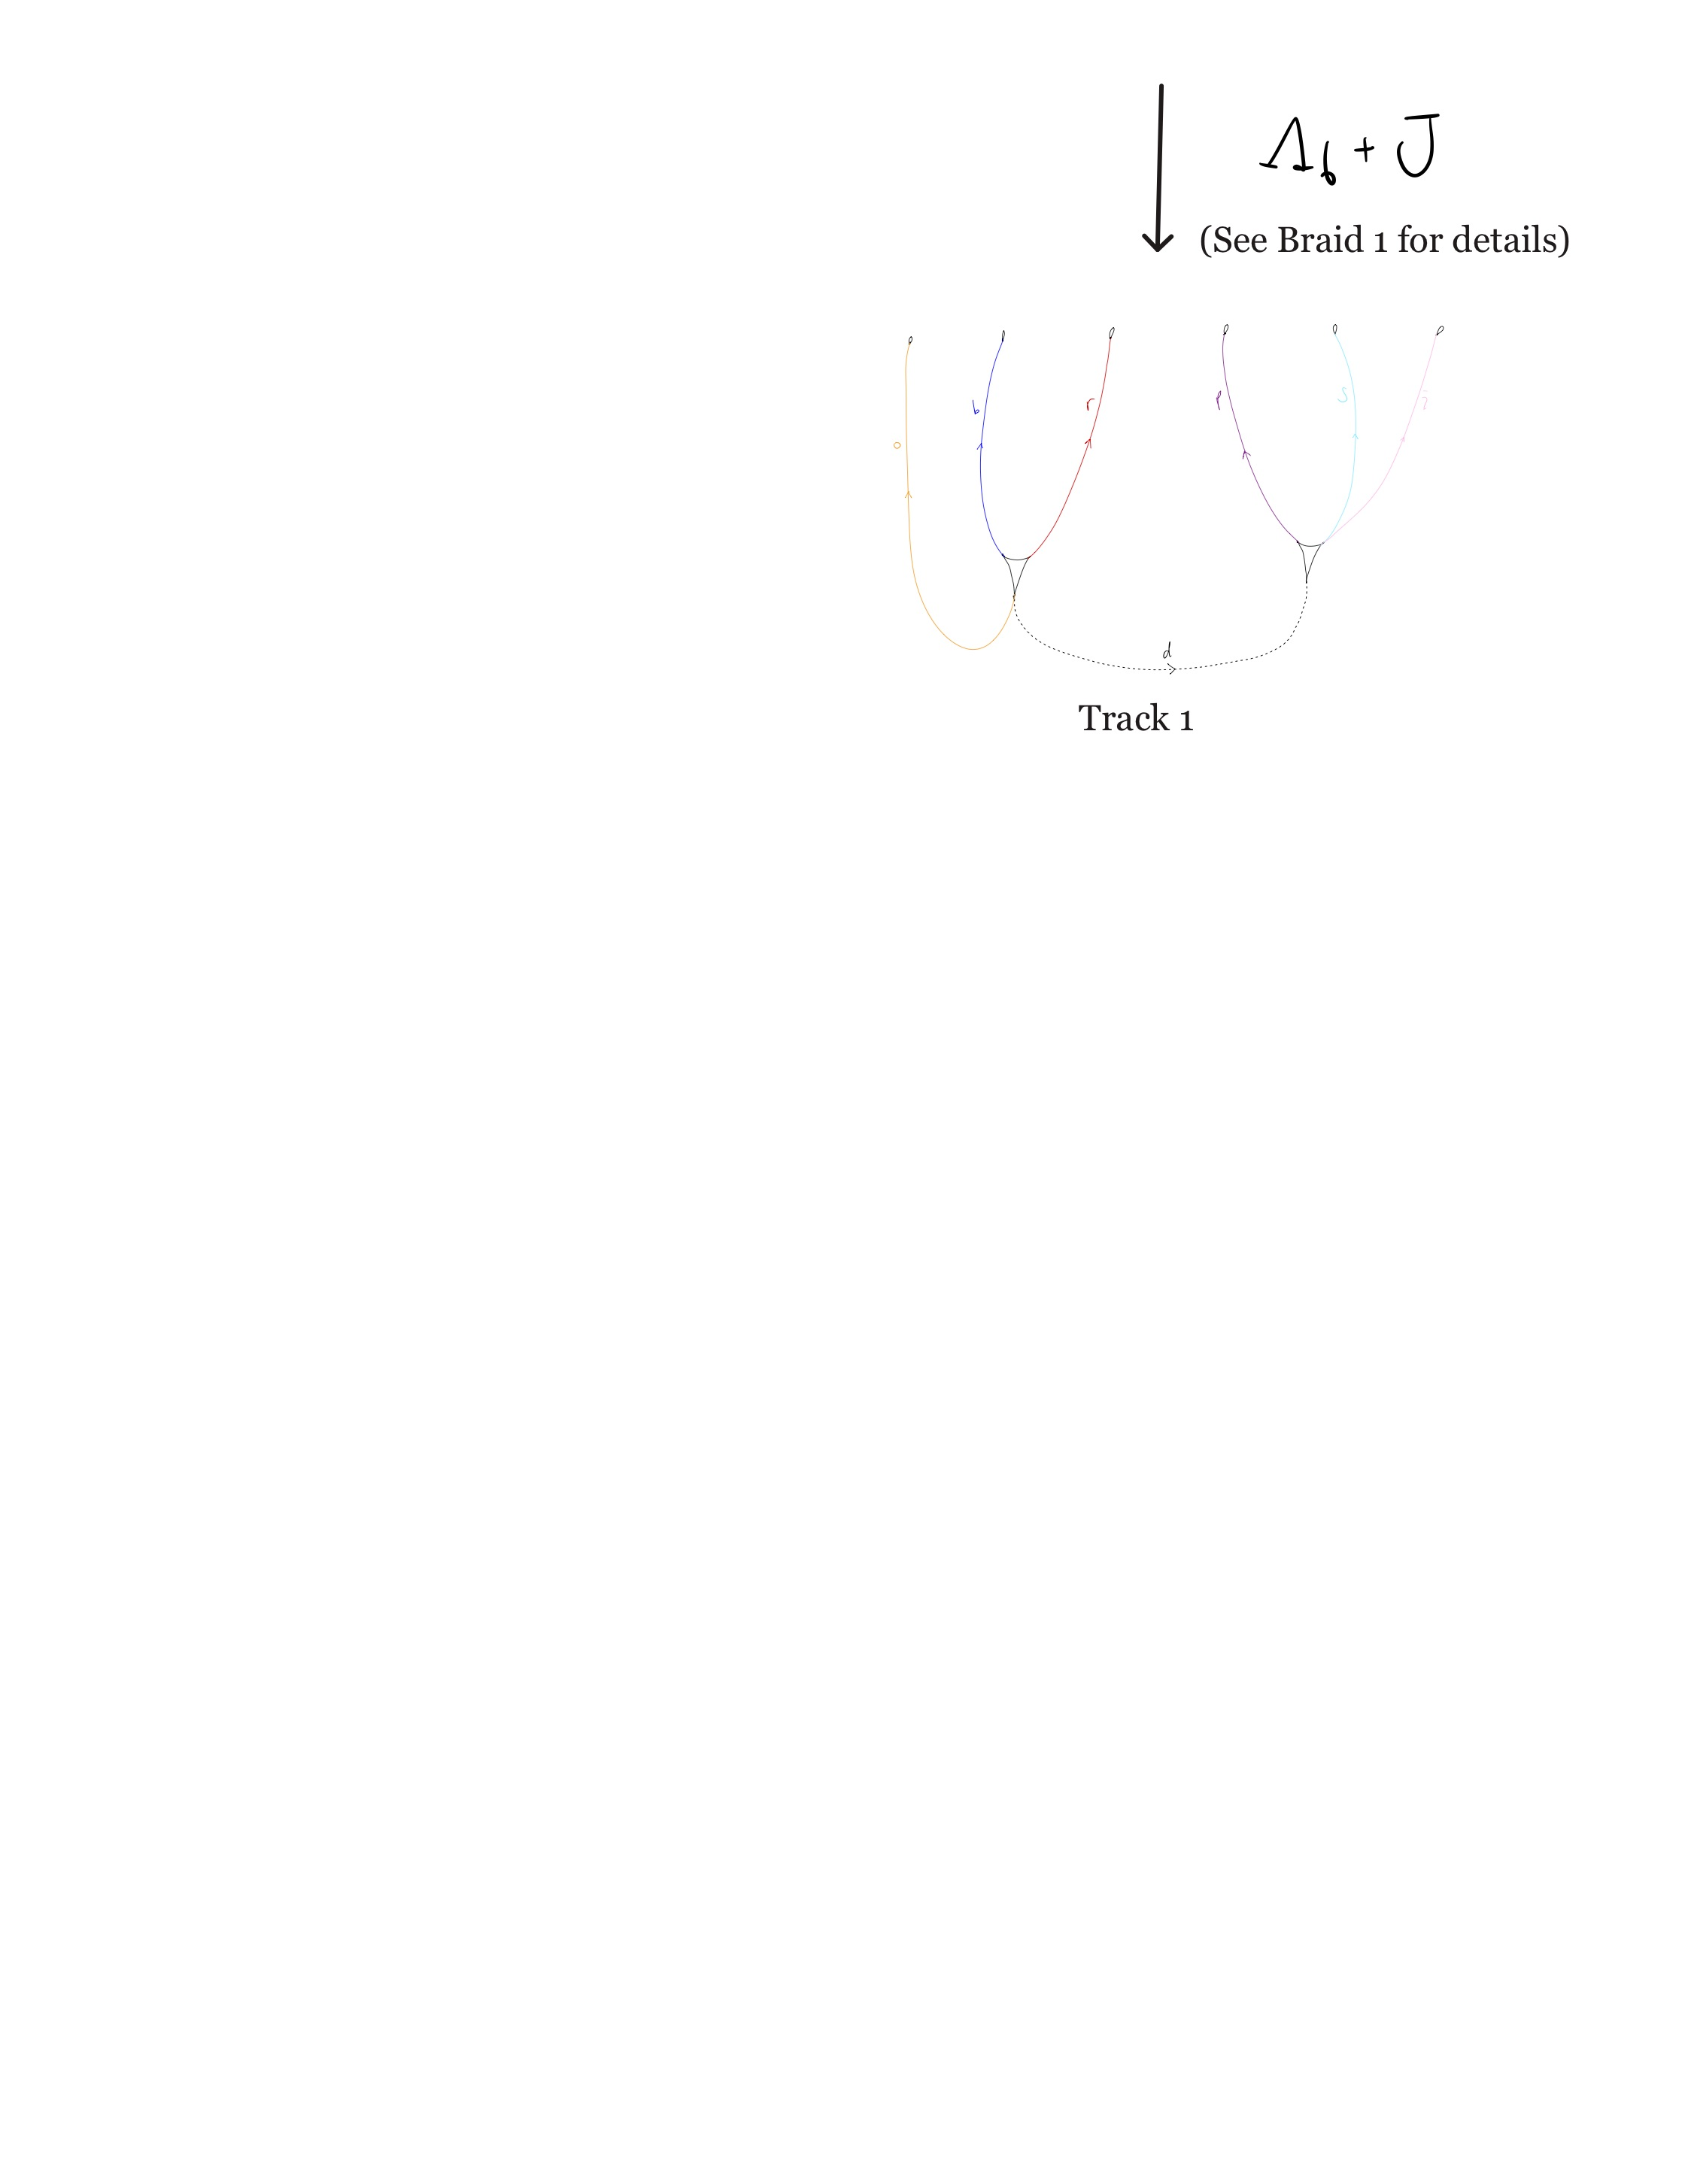
\includegraphics[width=\linewidth, height=0.45\textheight, keepaspectratio]{figures_braid/figures_track_1/Track 1 Braid 17 Popjoy-3.jpg}
    \caption{This sequence shows the inverse of the braid $b_{17}^1$ carries Train Track Candidate Family 17.}
    \label{fig:track1_braid_b1_17}
\end{figure*}

\clearpage